%\RequirePackage{snapshot}
% !TeX encoding = UTF-8
% !TeX spellcheck = en_GB
\documentclass[12pt,
%    draft,     %taking out draft switches marginal notes off and pictures on
    ]{book} 
\usepackage{incremental_SS_Translation} 
\addbibresource{incremental_SS_Translation.bib}
\usepackage{tabularray}
\UseTblrLibrary{booktabs}
%\DefTblrTemplate{firsthead, middlehead,lasthead}{default}{}
% private macros for switching between chapters    
\newif \ifkalpa \newif\ifsarira \newif \ifjvara \newif\ifsutra \newif\ifnidana
%
%\nidanatrue
\kalpatrue
%\sariratrue
%\sutratrue

\title{Draft Translation of the Nepalese Version of the \emph{Suśrutasaṃhitā}}

\author{Dominik Wujastyk 
    \and Jason Birch
    \and Lisa A. Brooks 
    \and Paras Mehta 
    \and Madhusudan Rimal
    \and Deepro Chakraborty
    \and Harshal Bhatt
    \and Jan Gerris
    \and et alii}
\date{\texttt{Draft of \today}\\ \copyright\ The Authors}

\newcommand{\ignoreargument}[1]{\empty }

\ifkalpa 
    \includeonly{%chapters/translation 5-introduction,
%    chapters/translation 5-introduction,
        chapters/translation 5-02,   
%        chapters/translation 5-06,   
%        chapters/translation 5-03,   
%        chapters/translation 5-08,   
        chapters/bibliography and indexes 
} \fi
%
\ifsutra
\includeonly{%chapters/translation 5-introduction,
    chapters/translation 1-13,    
    %chapters/bibliography and indexes
} \fi
\ifsarira \includeonly{%
   % chapters/translation 3-02,
    chapters/translation 3-01,
    % chapters/bibliography and indexes
} \fi       
%
\ifjvara  \includeonly{chapters/translation 6-39} \fi      
%  
\ifnidana \includeonly{chapters/translation 2-01,
    chapters/bibliography and indexes,
    } \fi

%
% from 
%https://tex.stackexchange.com/questions/361031/biblatex-how-to-automatically-sort-citation-by-year-sortcites-ynt-when-refere/361042#361042
\AtBeginRefsection{\GenRefcontextData{sorting=ynt}}
\AtEveryCite{\localrefcontext[sorting=ynt]}

\begin{document}
    
    \input{sanskrit-hyphenations}
        
    %\nocite{forb-1856}
    \pagecolor{cyan}
    \thispagestyle{empty}
          \maketitle

        \newpage
        \pagecolor{white}
        \tableofcontents
        
        \include{chapters/introduction}
            \thispagestyle{empty}
        
        \part{Part 1. Sūtrasthāna} 
                        
        % !TeX root = ../incremental_SS_Translation.tex

\chapter{Sūtrasthāna 1: The Origin of Medical Knowledge}

\section{Literature}

Meulenbeld offered an annotated overview of this chapter and a bibliography
of earlier scholarship to 2002.\fvolcite{IA}[203--204]{meul-hist} 

\section{Translation}

\begin{translation}
    
    \item[1] 
    
“Now I shall narrate the chapter on the origin of this
knowledge.\footnote{Ḍalhaṇa understood the word
    “\se{veda}{knowledge}" as specifically  “medical knowledge." He
    said that the word  “longevity" (\emph{āyur}) \ssaneng{āyur}{life,
    longevity} had been elided. %
    %    Notes Dec 8:
    %    Dominik: N's ādhyāyaṃ corruption of H's nāmādhyāyaṃ:
    % possible evidence that N was
    %created
    %after H
    %    Check: Ācārya 1931 footnote on vedotpattim
    %    Commentary Ḍalhaṇa (c. 1200 CE) notes āyur dropped from veda
    % in vedotpattim
    %
    %
    After this opening statement, later manuscripts and commentaries
    include the attribution,  “as the venerable Dhanvantari stated." 
    The absence of this statement in the early Nepalese manuscripts
    is highly significant because it removes the outer narrative
    frame of the \SS\
    \parencites[148]{wuja-2013}[\S\,3.1.2]{kleb-2021b}{rai-2019}{birc-2021}.  
    On the figure of Dhanvatari in medical literature, see \cite[IA 
    358--361]{meul-hist}.} %     <!-- Notes Dec 8:
    %    Dom: note the omission of Dhanvantari, which is in the
    % edition.
    %    On Dhanvantari, see Meulenbeld HIM, authorities associated
    % with Suśruta. He's
    % an authority on
    %surgery or toxicology-->
    
    \item[2] 
    
“Now, as is well-known, Aupadhenava, Vaitaraṇa, Aurabhra,
Puṣkalāvata, Karavīra, Gopurarakṣita, \diff{Bhoja}, Suśruta and
others addressed Lord Divodāsa, king of Kāśi, the best of the
immortals, who was in his ashram surrounded by an entourage of
sages.\footnote{On these persons, see \cite[IA 361--363,
    369\,ff.]{meul-hist}. \label{Bhoja}
    The authority Bhoja does not appear in the list
    as published in the vulgate edition \citep[1]{susr-trikamji2}, and
    was not included in \cite{meul-hist} amongst “authorities mentioned
    in the \SS.” \citeauthor{meul-hist} gathered textual evidence about
    Bhoja at \cite[IA 690--691]{meul-hist}. \citet{kleb-2021a} has
    discussed these authors in the context of an anonymous commentary on
    the \SS\ that cites them.}
    
    \nocite{emen-1969}
    
    %    Notes Dec 8:
    %    Dom: Check these names in Meulenbeld 
    %    Bhoja is an early lost authority on medicine. Not the same person as King Bhoja, 
    %commentator 
    %on the Yogasūtras.
    %    Ḍalhaṇa's comm. mentions Bhoja as also included in prabhṛtayaḥ: so the version of 
    %the text he 
    %was using did not mention Bhoja, but he was aware of him: His provenance makes it 
    %possible that 
    %he knew the Nepalese version of the SŚ
    
    \item[3]
    %O Lord, after seeing people who are assailed by the impingements of various pains 
    %caused by 
    %physical, mental and accidental diseases, who have the support of friends [but] 
    %feeling as if they 
    %were alone, and acting frantically, shouting out, we have been distressed. 
    
 “O Lord, distress arose in our minds after witnessing people
thrashing about with cries, assailed by different kinds of
\se{vedanābhighāta}{pain and injury}, feeling helpless in spite of
having friends, because of diseases arising from the body, the mind
and external sources.
    
    
    
    %    Notes Dec 8:
    %    āgantu - caused by something from outside the body
    %    abhighāta - threats, impingements 
    %    vedanābhighāta - tatpuruṣa 
    %    anātha - among a list of people who shouldn't be treated.
    %    Ḍalhaṇa- sanātha: samitra someone with a friend -->
    
    \let\uncertain\texttt
    
    \item[4] 
    
“To quell the illnesses of those who seek happiness and for our own
purpose of prolonging life, we desire \se{āyurveda}{the science of
    life} that is being taught. Welfare\ssaneng{śreyas}{welfare}, both in
this world and in the next, depends upon it. Therefore, we have come
to the Lord in pupillage." %
% reading bhagavan (voc.) and tam (it, ayurveda, masc. acc.)
    
    % we think upasannāḥ smaḥ is probably wrong, but we can't see how to improve it.
    % upapannā sma ?
    
    \item[5] 
    
The Lord said to them:
    
“Welcome to you!  My children, all of you are beyond reproach and
worthy to be taught.
    
    
    \item[6] 
    %     “As is well-known in this world, before creating people, Brahmā 
    %composed 
    %    what is called Āyurveda.\footnote{The relative pronoun \emph{yad}, that has 
    %no  
    %    correlative \citep[\P 461]{spei-1886}, is omitted.} 
    %    It is taught as part of the \emph{Atharvaveda}, in hundreds of 
    %    thousands of verses and a thousand chapters and, after observing the short 
    %    lifespan and low intelligence of people, made it again in eight parts. 
    %    %infer tat as the object of kṛtavān
    %    
    
“As is well known, Ayurveda is the name of what is said to be the
subsidiary part of the Atharvaveda.\footnote{On the careful wording
    of this statement, that makes the Atharvaveda connection “something
    that people say,” see \cite[400--401]{wuja-2022}.} Before creating
    people, Svayambhū composed it in hundreds of thousands of verses and
    a thousand chapters and, after observing the short lifespan and low
    intelligence of people, he presented it again in eight
    parts.\footnote{Svayambhū is another name for Brahmā, the creator.}
    
    \item[7] 
    
“Surgery, treatment of body parts above the clavicle, general
medicine, knowledge of spirits, care of children, and the disciplines
of antidotes, rejuvenation and aphrodisiacs. % why do some of the
% auxiliaries end in tantra? Dom: Some were disciplines that had a
%separate life outside āyurveda. The others were more particular
% to vaidyas.
    
    \item[8.1] 
    
“Now,  a collection of the characteristics of each component of
Āyurveda.
    
    \item[8.1a] 
    
“Among them, the one called surgery has the goal of extracting
various grasses, wood, stone, dust, iron,\footnote{The identity of
    the metal in such early literature is somewhat moot. For discussion,
    see \cite{wujad-2019}.} soil, bone, hair, nails, discharge of pus,
    malignant wounds and foreign bodies inside the womb, and of
    determining the application of surgical instruments, knives, caustics
    and fire by means of sixty definitions. %Ḍalhaṇa seems to read
    % duṣṭavraṇāntar, and glosses antar as madhyāt. He then reads
    %garbhaśalya (HIM - foetuses stuck in the womb). Ḍalhaṇa is aware
    % of the reading ṣaṣṭyā
    %vidhānaiḥ (following uddhraṇārtha), and says some explain it as
    % apatarpaṇādyai
    %rakṣāvidhānāntair dvivraṇīyoktair ity arthaḥ. However, mss. 699
    % and 533 read abhi° not
    %vi°
    
    \item[8.2] 
    
“The one named “the doctrine of treating body parts above the
clavicles” has the aim of curing diseases situated above clavicles
that is, diseases located in ears, eyes, mouth, nose and so on.
    
    \item[8.3] 
    
“The one called “general medicine” has the goal of curing
illnesses established in the whole body and [diseases] such as fever,
tumour, swelling, hemorrhagic disorders, insanity, epilepsy, urinary
diseases, diarrhoea and the like.
    
    \item[8.4] 
    
“The one called “knowledge of spirits” is for
appeasing demons by pacification rites and making food offerings
for those whose minds have been possessed by gods, their
enemies,\footnote{Dānavas.  The insertion marks
    (\emph{kākapada}s) below the text at this point appears to be by
    the original scribe.} Gandharvas, Yakṣas, demons, deceased
    ancestors, Piśācas, Vināyakas, \footnote{The vulgate doesn't have
        \emph{vināyaka}s but does add \emph{asura}s, probably under the
        influence of Ḍalhaṇa.}\q{Cite Paul Courtright, Ganesha book.}
        Nāgas and evil spirits that possess children. % Notes: vināyaka
        % is omitted from the vulgate. In
        % Mahābhārata, etc. It refers to
        %a class of demons.-->
    
    
    \item[8.5] 
    
“The one called “care of children” is for bearing children and
purifying defects in a wet-nurse's milk, and curing diseases that
have arisen from bad breast milk and demons.
    
    \item[8.6] 
    
“The one called “the discipline of toxicology” is for
    [knowing] the signs of poison from snake and insect bites and for
    neutralising various combinations of poisons.\footnote{The scribal
    insertion marks (crosses) above the line at this point in MS K appear to
    be in a later hand and their referent is lost in the damaged part of the
    folio.  Although MSS \MScite{Kathmandu NAK 1-1079} and \MScite{Kathmandu 
    NAK 5-333} include \se{lūtā}{spiders} and
    \se{sarīsṛpa}{creepy-crawlies} in the list, it does seem that MS K had
    a shorter list, and the vulgate edition adds \se{mūṣika}{rodents}.}
    
    \item[8.7] 
    
“The one called “the discipline of rejuvenation” is maintaining
youth, bringing about a long life and mental vigour and for curing
diseases.
    
    % Got to here 2021-01-13
    
    \item[8.8] 
    
“The one called the “discipline of aphrodisiacs”
brings about the increase, purity, accumulation and  production
of semen for those whose semen is minimal, bad, depleted, and dry
[respectively] and for inducing an erection.
    
    \item[9] 
    
“In this way, this Āyurveda is taught with eight components."
    
“Among these [components], tell us which is for whom."
    
    \item[10] 
    
They said,  “After you have \sse{alaṅkṛtvā}{made accessible}made the
whole knowledge of surgery accessible, teach it to us,
Lord”.\footnote{For discussion of the text-critical significance of
    this passage, see \cite{hari-2013}. I have read the passage as
    including the word \dev{alaṅkṛtvā} in the sense “make accessible”
    (\cite[cf.][94]{moni-sans}, \emph{sub} \dev{alaṃ vijñātum}.}
    
    \item[11]  “So be it," he said.
    
    \item[12] 
    
They then said,  “After probing our opinion, we are unanimous: Suśruta
will question you. We too will take in what is being taught to him."
    
 \item[13] 
 
“So be it," he said.

\subsection{In praise of surgery}    
    \item[14--16] 

“Now, as is well-known, the aim of Āyurveda is eliminating the
disease of one who has been assailed by disease and protecting the
healthy; Āyurveda is, “where they find a long life,” or “that by
which long life is known.” You should take in its best
\se{aṅga}{component}, which is being taught without conflicting with
tradition, perception, inference or analogy.
    
    \item[17] 
    
“For this component is first, the most important, because it is
referred to first; it cures wounds and joins together the most
important thing, Yajña's head. For, just as it has been said of old,
`the head that had been cut off by Rudra was joined again by the two
Aśvins.'
    
    \item[18] 
    
    “And also, of the eight disciplines of Āyurveda, alone is the best
because of the quick action of its \se{kriyā}{procedures}, its
application of blunt instruments, knives, caustics and fire, and
it is common to all disciplines.
    
    \item[19] 
    
"Therefore, it is eternal, meritorious, leads to heaven,
brings renown, bestows a long life, and affords a livelihood.
    
    \item[20] 
    
“This is what Brahmā said: `Prajāpati learned it. From him, the
Aśvins. From the Aśvins, Indra. From Indra, I. In this world, I will
transmit it to students, for the benefit of people.'
    
  \item[21]   
  
“There a verse about this:   
    \begin{sloka}
        For I am Dhanvantari, the first god, the remover of old age,
pain and death of mortals. Having understood surgery, the
best of the great knowledge systems, I arrived on earth again
to teach it here.\footnote{Note that this verse about the
    origin of surgery is the first place that the name
    “Dhanvantari” is introduced in the Nepalese version of the
    work. Dhanvantari is here identified with Brahmā, the creator
    of the world. For discussion, see \cite{birc-2021}.}
    \end{sloka}    
    
    % draft tr.
    
    \item[22] 
    
“In this context, as far as this discipline is concerned, a
\se{puruṣa}{human being} is called an amalgam of the five elements
and the embodied soul.  This is where \se{kriyā}{procedures} apply.
This is the locus.”
    
“Why?”
    
“Because of the duality of the world, the world is twofold: the
stationary and the moving. Its \se{ātmaka}{nature} is twofold,
depending on the preponderance of Agni and
Soma.\footcite[See][]{wuja-2004}  Alternatively, it can be considered
as being fivefold.  The multitude of beings in it are fourfold: they
are termed “sweat-born, stone-born, caul-born and
egg-born”.\footnote{This fourfold classification of beings is
    paralleled with closely-related vocabulary in  \emph{Bhelasaṃhitā}
    4.4.4 \parencites[206]{kris-2000}[81]{mook-1921}.}  Where they are
    concerned, the human being is the main thing; others are his support.
    Therefore, the \se{puruṣa}{human being} is the locus.
    
    \item[23--26]  

“Diseases are said to be the conjunction of the person and
\se{duḥkha}{suffering}. There are four of them: invasive, bodily,
mental and inherent.  The invasive ones are caused by an injury.  The
bodily ones are based on food, caused by
\se{vaiṣamya}{irregularities} in wind, bile, phlegm and
blood.\footnote{Note that four humoral substances are assumed here.}
    
“The \se{mānasa}{mental} ones, caused by 
    \se{icchā}{desire} and 
    \se{dveṣa}{hatred}, 
    include:  
    \se{krodha}{anger}, 
    \se{āśoka}{grief}, 
    \se{dainya}{misery}, 
    \se{harṣa}{overexcitement}, 
    \se{kāma}{lust}, 
    \se{viṣāda}{depression},
    \se{īrṣyā}{envy},
    \se{asūyā}{jealousy},
    \se{mātsarya}{malice}, 
    and
    \se{lobha}{greed}.
    
“The \se{svābhāvika}{inherent} ones are hunger, thirst, old age, death, 
    sleep and  those of the \se{prakṛti}{temperament}.
    
“These too are \se{adhiṣṭhāna}{located} in the mind and body.

\item[27]    

“\se{lekhana}{Scarification},
    \se{bṛṃhaṇa}{nourishment},
    \se{saṃśodhana}{purification},
    \se{saṃśamana}{pacification},
    \se{āhāra}{diet} and
    \se{ācāra}{regimen}, 
    properly employed, bring about their cure.
    
    
    \item [28] 
    
“Furthermore, food is the  \se{mūla}{root} of living beings as well as
of \se{bala}{strength}, \se{varṇa}{complexion} and \se{ojas}{vital
    energy}. It \se{āyatta}{depends on} the six \se{rasa}{flavours}.
Flavours, furthermore, have substances as their
\se{āśrayin}{substrate}.  And substances are
\se{oṣadhī-}{remedies}.\footnote{Pāṇini 6.3.132 provides that the
    final vowel of the noun \emph{oṣadhi} may be lengthened
    (\emph{$\rightarrow$oṣadhī}) under certain conditions.  These
    conditions require that the word be used in a Vedic mantra and not in
    the nominative.  Neither condition is met in this passage, yet the
    author uses the form \emph{oṣadhī}. This form is in fact not uncommon
    in medical literature as well as in epics, purāṇas, smṛtis, and other
    parts of Sanskrit literature.} There are two types:
    \se{sthāvara}{stationary} and \se{jaṅgama}{moving}.
    
    
    
    \item [29]  
    
“Of these, there are four types of stationary ones:
\se{vanaspati}{fruit trees}, \se{vṛkṣa}{flowering trees},
\se{oṣadhi}{herbs} and
\se{vīrudh}{shrubs}.\footnote{Ca.sū.1.71--72 also describes these
    four types of medicinal plant in similar terms but with slightly
    differing names: \emph{oṣadhi} is a plant that ends after
    fruiting, \emph{vīrudh} is a plant that branches out,
    \emph{vanaspati} is a tree with fruit, and \emph{vānaspatya} is a
    tree with fruit and flowers.} Amongst these, the “fruit trees”
    have fruit but no flowers.\footnote{The MSS agree in reading
        \emph{phalavantyaḥ} “having flowers” which is grammatically
        non-standard. This form is also found in the 
        \emph{Viṣṇudharmottarapurāṇa} (1.92.27,
        \cite[1.92.27][56r]{sarm-1912}).}  The “flowering trees” have
        flowers and fruit.  The “herbs” die when the fruit is ripe.
        “Shrubs” put out shoots.
    
    % \citep{ober-2003} didn't have anything on phalavantyo that I could find quickly.
    
    
    \item[30]  
    
“As is well known, moving remedies are also of four types: those
\se{jarāyuja}{born in in a caul}, those \se{aṇḍaja}{born from eggs},
those \se{svedaja}{born of sweat}, and \se{udbhid}{shoots}. Amongst
these, those born in a caul include \se{paśu}{animals}, humans, and
\se{vyāla}{wild animals}.  Birds, \se{sarīsṛpa}{creepy-crawlies} and
snakes are “born of eggs.” \se{kṛmi}{Worms}, \se{kunta}{small
    insects} and \se{pipīlika}{ants} and others are born of
sweat.\footnote{The word \emph{kunta}, though marked as “lexical” in
    most dictionaries, is in fact found in literature, commonly as a
    compound with \emph{pipīlika}; the compound sometimes seems to be
    understood a type of ant (\emph{tatpuruṣa} compound) rather than as a
    pair of insects (\emph{dvandva} compound).}  Shoots include
    \se{indragopa}{red velvet mites} and \se{maṇḍūka}{frogs}.\footnote{On
        \emph{indragopa}, see \cite{lien-1978}.}|
    
    \item[31] 
    
“In this context, among the stationary remedies, \se{tvak}{skin},
\se{patra}{leaves}, \se{puṣpa}{flowers}, \se{phala}{fruits},
\se{mūla}{roots}, \se{kanda}{bulbs}, \se{kṣīra}{sap},
\se{niryāsa}{resin}, \se{sāra}{essence}, \se{sneha}{oil}, and
\se{svarasa}{juice extract}\footnote{On \se{svarasa}{juice extract}
    see CS 1.1.73, 1.4.7; Ḍalhaṇa on \Su{4.10.12}{450}.} are useful;
    among the moving remedies \se{carman}{pelt}, hair, nails, and
    \se{rudhira}{blood} and so forth.
    
    \item[32] 
    
“And \se{pārthiva}{earthen products} include gold and
silver.\footnote{The flow of concepts in the treatise seems to be
    interrupted here.}
    
    \item[33] 
    
“The \se{kālakṛta}{items created by time} are \se{samplava}{clusters}
as far as wind and \se{nivāta}{no wind}, heat and shade, darkness and
light and the cold, hot and \se{varṣā}{rainy seasons} are concerned.
The divisions of time are the \se{nimeṣa}{blink of the eye}, a
\se{kāṣṭhā}{trice}, \se{kalā}{minutes}, \se{muhūrta}{three-quarters
    of an hour}, a \se{ahorātra}{day and night}, a \se{pakṣa}{fortnight},
a \se{māsa}{month}, a \se{ṛtu}{season}, a \se{ayana}{half-year}, a
\se{saṃvatsara}{year}, and \se{yuga}{yuga}.\footnote{These units are
    presented at \Su{1.6.5}{24} and discussed by
    \citet[\S\,59]{haya-2017}.}
    
    
    \item[34] 
    
“These naturally cause 
    \se{sañcaya}{accumulation}, 
    \se{prakopa}{irritation}, 
    \se{upaśama}{pacification} 
    and 
    \se{pratīkāra}{alleviation} of the \se{doṣa}{humours}. And they have
    \se{prayojanavat}{practical purposes}.
    
   
    
    \item[35] 
    
“There are verses about this:
     \begin{sloka}
        This fourfold category is taught by physicians as a cause for the agitation and 
        quelling of bodily diseases.%
        %
        \footnote{On the topic of the “group of four,” the commentator Ḍalhaṇa
        considered them to be “food, behaviour, earthen products and items 
        created by
        time.”  He referred to the author of the lost commentary entitled 
        \emph{Pañjikā},
        and to Jejjaṭa \citep[IA, 372--3, 192]{meul-hist}.  In his view, these early
        commentators  do not agree that the \se{caturvarga}{fourfold grouping} 
        refers
        to the quartet of \se{sthāvara}{stationary}, \se{jaṅgama}{moving},
        \se{pārthiva}{earthen products} and \se{kālakṛta}{items created by 
        time} \citep[9a]{vulgate}.}
    \end{sloka}
    

    \item[36] 
    
    \begin{sloka}
        There are two kinds of invasive diseases. Some certainly\footnote{The
        text uses an archaic interjection here, \emph{ha}.} 
        affect (\emph{ni$\surd$ pat}) \index{nipat@ni$\surd$ pat}
        the
        mind, others the body. Their \se{kriyā}{treatment} is of two kinds too.
    \end{sloka}
    
    \item[37]
    
    \begin{sloka}
        For those that affect the body there is \se{śārīravad}{physical} 
        therapy, whereas for those that affect the mind there is the 
        \se{varga}{collection} of desirable sensory experiences like sound that 
        bring \se{sukha }{comfort}.    
    \end{sloka}
    %Those that affect the body have therapy that is  
    %\se{śārīravat}{physical}, whereas for those of the mind it is 
    
    \item [38] 
    
“\se{evam}{Along these lines}, this brief explanation of the 
    \se{catuṣtaya}{four factors}
    is given: \begin{itemize}
        \item    
        \se{puruṣa}{human being},
        \item
        \se{vyadhi}{disease},
        \item
        \se{oṣadhi}{remedies},
        \item
        \se{kriyākāla}{the time for therapies}.
    \end{itemize}
“In this context, 
    \begin{itemize}
        \item from the mention of the word “human,” the collection of 
        substances that arise from it, such as the elements, and the 
        \se{vikalpa}{particulars} of its major 
        and minor \se{aṅga}{parts} such as 
        \se{tvak}{skin}, 
        \se{māṃsa}{flesh}, 
        \se{sirā}{ducts}, 
        \se{snāyu}{sinews}, 
        \se{asthi}{bones} and 
        \se{sandhi}{joints}
        are meant.
        \item
        From the mention of “diseases,” all diseases 
        caused by
        wind, bile, phlegm,
        \se{sannipāta}{congested humours},
        \se{āgantu}{external factors} and 
        \se{svabhāva}{inherent factors} are \se{vyākhyāta}{intended}.
        \item
        From the mention of “remedies,”
        there is the teaching of 
        substances,
        tastes, 
        potencies,
        post-digestive tastes.
        \item
        From the mention of 
        “\se{kriyā}{procedures},”
        \se{karman}{therapies} such as oiling
        and 
        \se{chedya}{excision} are taught.
        \item
        From the mention of the word “time,” every single teaching about the times for
        procedures is meant.        
    \end{itemize}
  
    
    \item[39]
    
 “There is a verse about this:
    \begin{sloka}
        This seed of medicine has been declared in brief.  Its explanation will be given in one 
        hundred and twenty chapters.\footnote{This is the number of chapters in the first 
        five sections of the work, namely the  \emph{Sūtra-, Nidāna-, Śārīra-, Cikitsā-} 
        and \emph{Kalpa-sthāna}s. These have 46, 16, 10, 40 and 8 chapters respectively.  The 
        \emph{Uttaratantra} has 66 chapters.}
\end{sloka}

%[There are verses on this:]\q{is this bha
%really in the MSS?}

\item [40] 

“There are one hundred and twenty chapters in five
\se{adhyāya}{sections}.\footnote{On \emph{viṃśa} in the sense of
    “greater by 20” see P.5.2.46 \emph{śadantaviṃśateś ca}.}  In that
    regard, having divided them, according to their subject matter, into
    the Ślokasthāna, the Nidāna, the Śārīra, the Cikitsita and the Kalpa,
    we shall mention this in the Uttaratantra.\footnote{The end of this
        sentence reads oddly.  The vulgate edition adds an object: “[we shall
        mention] the remaining topics [in the Uttara]” which smooths out the
        difficulty, but this is supported in none of the Nepalese MSS.  At
        the start of the Uttaratantra \citep[1.3--4ab]{vulgate} there is
        indeed a statement that picks up the point about there being 120
        chapters.}


\item[41]    

“There is a verse about this:
\begin{sloka}
    Someone who reads this eternal proclamation of the King of
    Kāśī, that was declared by Svayambhu, will have good karma on earth, will
    be respected by kings and upon death will achieve the world of Śakra.
\end{sloka}

\end{translation}    

            \thispagestyle{empty}
        \include{chapters/translation 1-02}
            \thispagestyle{empty}
        \include{chapters/translation 1-03}
            \thispagestyle{empty}
        \include{chapters/translation 1-10} % diagnosis
            \thispagestyle{empty}
        \include{chapters/translation 1-11} % preparing caustics
\thispagestyle{empty}        \include{chapters/translation 1-13} % leeches
            \thispagestyle{empty}
        % !TeX root = ../incremental_SS_Translation.tex

\chapter{Sūtrasthāna 14:  On the Properties of Blood}


\subsection{Literature}

Meulenbeld offered both an annotated summary of this chapter as well as a
study specifically on the place of blood in Ayurvedic
theory.\footnote{\volcite{IA}[209--201]{meul-hist}  and \cite{meul-1991}.
    Meulenbeld's footnotes on this chapter in
    \volcite{IB}[325\,ff.]{meul-hist} refer often to ``Hoernle's note.'' 
    This appears to be a reference to Hoernle's copious notes to his
    translation of this chapter \citep[87--98]{hoer-1897}. \citet{meul-1990}
    also discussed Sanskrit veterinary texts in the light of their standard
    theory of four humours, including blood.}

\subsection{Translation}

The draft translation of this adhyāya is presented by Paras Mehta.

\begin{translation}    
\item [1] Now we shall declare the chapter about blood.

\item [2]

    %\cite[33]{adri-1984} -> Author 1999: 33
    
\item [3] Food is of four types.\footnote{\label{fourfoods}Ḍalhaṇa on \Su{1.14.3}{59} said
    that the four types of food are those that can be drunk, licked, eaten
    and chewed(\dev{peyalehyabhojyabhakṣya}). The main text of the \CS\ is
    explicit about these categories at \Ca{4.3.4(1)}{308}:
    \dev{pānāśanabhakṣyalehya/} “things drunk, eaten, chewed or licked.”
    \citet{yagi-1994} discussed the distinction between \dev{bhakṣya} and
    \dev{bhojya}; for further Indological background on foods, see the
    studies by \citet{oliv-1995,oliv-2001} and the classic reference works by
    \citet{acha-1994,acha-1998}. The long, final adhyāya of the
    \SS's sūtrasthāna (ch.\,46) amounts to a distinct treatise on food in 
    āyurveda.} It is endowed 
    with six tastes and is made
    of the five elements.\footnote{\emph{Idem}, earth, water, fire, air,
        space} It has either two or eight potencies, and is endowed with many
        qualities. \footnote{Ḍalhaṇa related these qualities to the twenty
            standard \dev{guṇa} of āyurveda; see, e.g., their listing by Vāgbhaṭa,
            translated by \citet[207]{wuja-2003}. }
            \se{rasa}{Chyle} is the most intangible essence of this food that is
            properly transformed. It is of the nature of fire.
                
Chyle is situated in the heart. From the heart, it enters into the
twenty-four arteries—ten upward arteries, ten downward, and four
sideways—and doing so day after day owing to the reaction of past
activities that are caused by the invisible,\footnote{\dev{adṛṣṭa}
    (unseen): Doing any righteous or unrighteous action produces good merit
    and demerit respectively. This good merit and demerit are called
    \dev{adṛṣṭa} (invisible) because it cannot be directly known but can only
    be assumed through logical deduction.} it satisfies the entire body,
    enlivens it, prolongs it,\footnote{In the sense of prolonging its
        lifespan} and makes it grow. The motion of the entity that flows
        throughout the body should be understood by inference. That motion causes
        deterioration and growth.
    
With regards to the chyle that flows through all the limbs, humours, body tissues, 
and impurities of the body, the question arises, “Is it moist or is it fiery?” It is 
understood to be moist because of its fluidity while flowing\footnote{The vulgate 
emends \dev{anusaraṇe} to \dev{anusaraṇa-} against the Nepalese MSS. This is 
logical because mobility would seem to be one of the attributes.  Although it is 
awkward, we read \dev{anusaraṇe} as a locative absolute ``while flowing.''} and 
due to attributes such as mobility, lubrication, enlivening, satisfaction, and 
supporting.\footnote{The duality being discussed here is that of the essential 
qualities of Fire and of Soma (\emph{agni} and \emph{soma}). See further 
discussion by \citet{wuja-2004} and \citet{ange-2021}.}
    
\item [4]  
That watery chyle is then reddened after reaching the liver and spleen.

  
\item [5]
There are verses about this.

\begin{sloka}
Experts know that blood is the untransformed fluid that is reddened by the pure fire element within the bodies of living beings. %[by them??].
% Transcription of vulage has the verse divided into two IDs. They have to be combined into one.
\end{sloka}

\item [6]

\begin{sloka}
It is only due to chyle that women's blood called menses exists. It increases from the twelfth year and decreases after the fiftieth year. 
\end{sloka}

\item [7]

The menstrual blood, however, is called fiery.\footnote{Ḍalhaṇa commented that this is to distinguish the menstrual blood from regular blood that is gentle.} That is due to the embryo being fiery and moist.\footnote{Ḍalhaṇa commented here that the embryo is called such 
because the menstrual blood is fiery and the semen is gentle (\dev{saumya}). On  the fiery/moist distinction (\dev{āgneya/saumya}), see \cite{wuja-2004,ange-2021}.}

%\footnote{\dev{agnīṣomīya} is a 
%particular Vedic sacrifice which is related to the deities of fire (\dev{agni}) and 
%moon (\dev{soma}). Ḍalhaṇa commented that the embryo is called such 
%because 
%the menstrual blood is fiery and the semen is gentle (\dev{saumya}). The word 
%\dev{saumya} is derived from the word \dev{soma}, where it means that 
%which 
%has the qualities of the moon, i.e. that which is gentle. }

\item [8]

Others state that the embryo as constituted of the five elements and the preceptors call it the living blood. 

\item [9]
There are verses about this.
\begin{sloka}
That is because blood exhibits the qualities of earth, etc. such as a fleshy smell, 
fluidity, redness, pulsation and thinness.
\end{sloka}

\item [10]

\begin{sloka}
Blood is formed from chyle, flesh from blood, lymph from flesh, bone from lymph, marrow from bone, semen from marrow, and progeny from semen. 
\end{sloka}

\item [11]

There, the essence (chyle) of food and drink is the nourisher of these body tissues.


\item[12]

There is a verse about this.

\begin{sloka}
A living being should be known as born from chyle. One should diligently preserve\footnote{All three manuscripts have \dev{rakṣeta} which is an incorrect form. \dev{rakṣet} is the correct form.} chyle by administering food and drink, being nicely disciplined with food\footnote{\dev{āhāreṇa} - The third case is used. The semantic property of the third case used here is unclear. Unclear regarding if there is any rule in the \emph{Aṣṭādhyāyī} justifying this usage.}.
\end{sloka}

\item[13]

The verbal root \emph{rasa} means movement.\footnote{\cite[109]{bhis-1907}} Because it keeps moving day after day, it is called \emph{rasa} (chyle).\footnote{In the list of verbal roots of Pāṇini, the verbal root \dev{rasa}(\emph{rasa}) means taste and moistening. It does not mean movement.}    

\item[14]

Chyle stays in every body tissue for 2548 ((25*100)+48) \emph{kalās} and nine \emph{kāṣṭhas}. As such, it becomes semen after a month. For women, it becomes menses.  

\item[15] 
Here are verses about this.

\begin{sloka}
According to similar and dissimilar treatises, the quantity of \emph{kalās} in 
this group\footnote{The duration of chyle in all the body tissues as a whole.} 
is 18,090.

%\item[15ef-gh]

This is the particular transformation period regarding chyle that lasts for a person with mild fire\footnote{Perhaps this refers to the digestive fire.}. For a person with developed fire, one should know it to last for the exact same time\footnote{Although the vulgate does not have this verse, there is an argument presented in Ḍalhaṇa's commentary on \Su{1.14.16}{63} that for a person with intense fire, chyle becomes semen after eight days, and for a person with mild fire, chyle becomes semen after a month. Ḍalhaṇa said that this opinion is refuted by Gayadāsa Ācārya in many different ways. Ḍalhaṇa continued that the proper understanding is that for a person with a strong fire, chyle becomes blood in a little less than a month, and for a person 
with a mild fire, chyle becomes blood in a little more than a month.}
%This particular transformation in chyle comes to an end due to the mild fire. Also, in the same duration of time, that\footnote{The end of transformation of chyle} is to be known due to the grown/big/manifest fire.

%OR

%This particular transformation in chyle forms the end due of the mild fire. Also, in the same duration of time, that of the intense fire is to be known.
\end{sloka}

\item[16]

Resembling the expanse of sound, flame, and water, that entity moves
along in a minute manner throughout the  entire body.\footnote{Ḍalhaṇa
    comments \citep[63]{vulgate} that the expanse of sound indicates the
    sideways movement of chyle, the expanse of flame indicates the upward
    movement of chyle, and the expanse of water indicates the downward
    movement of chyle. On \dev{aṇunā viśeṣeṇa} “in a minute manner” see
    footnote \ref{anuna-visesena}.}

\item[17]

The aphrodisiac medicines, however, being used like a purgative due to their excessively strong characteristics, evacuate the semen.      

\item[18]

Just as it cannot be said that the fragrance in a flower bud is present in it or not, but 
accepting that there is the manifestation of existing entities\footnote{This is the 
doctrine of pre-existence of the effect (\dev{satkāryavāda}, \textit{satkāryavāda}) 
first propounded by Sāṅkhya philosophers.}, it,\footnote{fragrance} however, is not 
experienced only due to its intangibility. That same entity is experienced at another 
time in the blossomed flower. In the same way regarding children also, the 
manifestation of semen happens because of the advancement of 
age\footnote{Since chyle becomes semen in a month's time, a question arises "Why 
then is semen absent in young children?". The reply is given in this passage.}. For 
women, the manifestation is different as rows of hair, menses, etc. 

\item[19]

That very essence of food does not nourish very old people due to their decaying bodies.

\item[20]

These entities are called body tissues (\emph{dhātu-s}) because they bear the body\footnote{The etymological meaning of the Sanskrit word \dev{dhātu} (\emph{dhātu}) is "that which bears [the body]". Thus, the body tissues are called \emph{dhātu-s} because they bear the body. This means that the body tissues are the elements that make up the body and sustain it.}. 

\item[21]

Their decay and growth are due to blood. Therefore, I will speak about blood. 
In that regard: The blood that is foamy, tawny, black, rough, thin, quick-moving, and non-coagulating is vitiated by air. The blood that is dark green, yellow, green, brown, sour-smelling, and unpleasant to ants and flies is vitiated by bile. The blood that is orange, unctuous, cool, dense, slimy, flowing, and resembling the colour of flesh-muscles is vitiated by phlegm. The blood having all these characteristics is vitiated by the combination of all three of them. The blood that is extremely black is vitiated by blood\footnote{\citet[64]{vulgate} quote Cakrapāṇidatta in a footnote: "This is the symptom when the blood vitiated in one part of the body vitiates the blood in another part."} just as bile. The blood that has the combined characteristics of vitiations of two humours is vitiated by two humours.

\item[22]

The blood that is of the colour of insect cochineal, not thick, and not discoloured should be understood to be in its natural state. 

\item[23]

I will speak of the types of blood that should be let out in another section. 

\item[24]

Now, I speak of those that should not be let out.
The swelling appearing in all the limbs of the body of a weak person that happens due to consuming sour food. The swellings of people with jaundice, piles, large abdomen, emaciation, and those of pregnant women.

\item[26]

In that regard, one should quickly insert the surgical instrument that is simple, not very close, fine, uniform, not deep, and not shallow. 

\item[26a] 
One should not insert the instrument into the heart, lower belly, anus, navel, waist, groins, eyes, forehead, palms, and soles.

\item[26b]

In the case of swellings filled with pus, one should treat them in the same way as stated earlier.

\item[27-27a]

There, when the swelling is not pierced properly, when phlegm and air have not been sweated out, after having a meal, and due to thickness, the blood does not ooze out or oozes out less.
Here is a verse regarding it.

\item[28ab-cd]

\begin{sloka}
Blood does not ooze out of humans when in contact with air, passing stool or urine, and when intoxicated, unconscious, fatigued, sleeping, or in cold surroundings.
\end{sloka}

\item[29] 

That vitiated blood when not taken out increases the disease.

\item[30]

The blood that is let by an ignorant physician in cases of very hot surroundings, profuse perspiration, and excessive piercing, flows excessively. That profuse bleeding causes the appearance of acute headache, blindness, and partial blindness, or it quickly causes subsequent wasting, convulsions, tremors, hemiplegia, paralysis in a limb, hiccups, coughing, panting, jaundice, or death.  

\item[31ab-cd]

The physician should let out the blood when the weather is not very hot or cold, when the patient is not perspiring or heated up, and after the patient has had a sufficient intake of gruel. 

\item[32ab-cd]

After coming out properly, when the blood stops automatically, one should know that blood to be pure and drained properly.

\item[33ab-cd]

The symptoms of the proper drainage of blood are the experience of lightness, alleviation of pain, a complete end of the intensity of the disease, and satisfaction of the mind.

\item[34ab-cd] 

Defects of the skin, tumours, swellings, and all diseases caused by blood never arise for those who regularly drain their blood.

\item[35]

	When the blood does not flow out, the physician should rub cardamom and camphor on the opening of the boil with three or four or all among crêpe ginger (Cheilocostus speciosus), butterfly gardenia (Ervatamia coronaria Stapf), \gls{pāṭhā}, \gls{bhadradāru}, \gls{viḍaṅga}, \gls{citraka}, the three spices (black pepper, long pepper, and dry ginger), \se{āgāradhūma}{soot from the chimney}, turmeric, sprouts of \gls{arka}, and fruit of the \gls{naktamāla}, according to availability, with excessive salt. By doing so, the blood flows out properly.

\item[36]

When there is an excessive flow of blood, the physician should sprinkle the 
opening of the boil with dry powders of \gls{lodhra}, liquorice, \gls{priyaṅgu}, 
\gls{pattāṅga}, red chalk, \gls{rasāñjana}, seashell, barley, \gls{māṣa}, 
wheat, and resin of the Sāla tree, and then press it with the tip of a finger. 
One should tightly bind it with powdered barks of Sāla, \gls{sarja}, \gls{arjuna}, \gls{arimeda}, \emph{granthi}, \gls{dhava}, and \emph{dhanvana} (Camelthorn), or a linen cloth\footnote{\cite[66]{vulgate} has \dev{kṣaumeṇa vā dhmāpitena} - "with linen reduced to ashes". Presumably, it is this ash that is also referred to in item 40.}, or \emph{vadhyāsita}, or bone of cuttlefish, or powdered lac, along with the binding materials mentioned. 
After the piercing, the physician should pierce it again. 
The physician should serve cool clothing, food, a dwelling place, a bath, cooling 
ointments, and plastering. Or, one can cauterize
%\footnote{Cauterization: The use of 
%heat to destroy tissues or close minute bleeding vessels.(Reference: 
%https://medical-dictionary.thefreedictionary.com/cauterization)} 
it with heat. Or, as 
mentioned, one should give a decoction of \emph{kākolī}, etc. sweetened by sugar and honey to drink. 
Or, one should consume the blood of black buck, deer, ram, buffalo, rabbit, or pig, accompanied by milk, green gram soup and meat soup\footnote{Based on Ḍalhaṇa's comment as found in \cite[66]{vulgate}}. 
The physician should treat the pains as mentioned. 

\item[36a]

Here are verses about this.

\item[37ab-cd]

\begin{sloka}
When blood flows out due to the decay of body tissue, fire becomes weak\footnote{This refers to the digestive fire.} and the wind becomes highly agitated because of that endeavour.
\end{sloka}

\item[38ab-cd]

\begin{sloka}
The physician should serve the patient food that is not very cold, light in digestion, unctuous, increases blood, slightly sour or not sour at all. 
\end{sloka}

\item[39ab-cd]

\begin{sloka}
This is the four-fold method of hindering blood: joining, coagulation, 
haemostasis.
%\footnote{Deliberate arrest of bleeding by local compression or 
%clamping of bleeding vessels...(Reference: 
%https://medical-dictionary.thefreedictionary.com/haemostasis)}, 
and cauterization.  
\end{sloka}

\item[40ab-cd]

\begin{sloka}
The astringent substance joins the opening, the cold substance coagulates the blood, the ash stops the blood, and cauterization contracts the blood vessel.
\end{sloka}

\item[41ab-cd]

\begin{sloka}
If the blood does not coagulate, the physician should employ joining. If the blood does not stop by joining the opening then he should employ haemostasis.
\end{sloka}

\item[42ab-cd]

\begin{sloka}
The physician should endeavour by employing these three methods according to the procedure. If these methods are unsuccessful then cauterization is highly desirable.
\end{sloka}

\item[43ab-cd]

\begin{sloka}
If the blood remains impure, the disease does not aggravate. The physician should 
then make the blood pure\footnote{Ḍalhaṇa comments \citep[66]{vulgate} that 
one should purify the blood again by sedation, etc.}\q{Can't be “sedation”} and not 
drain blood in excess.
\end{sloka}

\item[44ab-cd]

\begin{sloka}
Blood is the basis of the body. It is sustained by blood only.
\end{sloka}

\item[44ef]

\begin{sloka}
Blood is called life. One should therefore save blood.
\end{sloka}

\item[45ab-cd]

\begin{sloka}
If the air in the person who underwent blood-letting is aggravated due to a cold shower, etc., the swelling with pricking pain should be sprinkled with lukewarm clarified butter.   
\end{sloka}

\end{translation}

 % blood
            \thispagestyle{empty}
       % !TeX root = ../incremental_SS_Translation.tex

\chapter{Sūtrasthāna 16: Repairing Pierced Ears}

\section{Literature}

Meulenbeld offered an annotated overview of this chapter and a
bibliography of earlier scholarship to
2002.\fvolcite{IA}[211--212317]{meul-hist}  A book on this topic, arising
out of the present project, with edition, translation and discussion of
the Nepalese transmission is published by \cite{wuja-2023}.


\section{Translation}

\begin{translation}    
  
\item [1] 

Now we shall expound the method for piercing the ear.\footnote{The topic of 
    \se{kaṛnavyadha}{piercing the ear} is not discussed in the \emph{Carakasaṃhitā}
    (\cite[IB, 326, n.\,175]{meul-hist}), but it is mentioned in some texts that
    followed the \emph{Suśrutasaṃhitā}, such as the \emph{Kaśāpyasaṃhitā} \citep[IIA,
    30]{meul-hist}. Also, the instrument for piercing the ear is described in the
    \emph{Aṣṭāṅgahṛdayasaṃhitā} \Ah{1.26.26}{321}. In the versions of the text known
    to Ḍalhaṇa \citep[76]{vulgate} and Cakrapāṇidatta \citep[125]{acar-1939}, the
    heading of this chapter is “the method of piercing and joining the ear”
    (\dev{karṇavyadhabandhavidhi}), instead of the Nepalese version's “the method of
    piercing the ear” (\dev{karṇavyadhavidhi}). The topic of joining the ear
    (\dev{karṇabandha}) is discussed in passages 17--20 of the Nepalese version.
    However, it appears that only subsequent redactors reflected its importance by
    including it in chapter headings.

 The Nepalese version also omits the opening remark on Dhanvantari that appears in
subsequent versions of the text. For a discussion of the frame story in the
Nepalese version, see \cite{birc-2021}. 

When commenting on this statement, Ḍalhaṇa \citep[76]{vulgate} and
Cakrapāṇidatta \citep[125]{acar-1939} observed that only the ears of healthy
people should be pierced, and they quoted the lost authority Bhoja to affirm
this: “When piercing the ears of children who are free of disease at these
times, their ear flaps and apertures, as well as limbs, increase” (\Su{1.16.1}{76}).

Some texts use the adjective \dev{karṇa-vedhanī} rather than \dev{°vyadhanī}.}

\item [2] 

One may pierce a child's ears for the purpose of preserving and decorating. During the
bright fortnight, when the child is in the sixth or seventh month, on renowned
days, half days, hours and constellations, the physician, with a calming presence,
sits the boy, who has received a benediction and the recitation of a
blessing,\footnote{The causative form \dev{vyadhayet} is known in Classical
    Sanskrit \citep[166]{whit-root}.

The compound \dev{kṛtamaṅgalasvastivācanaṃ} “who has received a benediction and
the recitation of a blessing” is an emendation based on the similar text at
\Su{3.2.25}{346}.  Cf.\ also \Su{3.10.8, 24}{388, 390} that have slightly
different formulations.} on the lap of a wet-nurse.\footnote{The versions of
    1.16.3 known to Cakrapāṇidatta \citep[126]{acar-1939} and Ḍalhaṇa
    \citep[76]{vulgate} have the additional compound \dev{kumāradharāṅke} (“on the
    lap of one who holds the child”) after \dev{dhātryaṅke}. The gender of
    \dev{kumāradhara} is made clear by  Ḍalhaṇa's gloss “a man who holds the child.”
    Also, both versions add \dev{bālakrīḍanakaiḥ pralobhya} (“having enticed with
    children's toys”) to indicate that the child should be tempted with toys to stay
    on the assistant's lap. According to Ḍalhaṇa on \Su{1.16.3}{76}, the toys include
    replica elephants, horses, bulls and parrots. Ḍalhaṇa further mentions that others
    read \dev{bhakṣyaviśeṣairvā} (“or by special treats”) before
    \dev{bālakrīḍanakaiḥ}, but we see no trace of these small kindnesses in our
    witnesses.} Then, he should pull the ear with his left hand 
    and pierce straight through with his right hand at a naturally-occurring
    cleft.\footnote{The versions of 1.16.3 of Cakrapāṇidatta \citep[126]{acar-1939}
        and Ḍalhaṇa \citep[76]{vulgate} add that this naturally-occurring cleft is
        illuminated by a ray of sunshine  (\dev{ādityakarāvabhāsite}).

The syntax of this slightly long sentence is unusual because of the dual
object \dev{tau} “the two (ears)” at the start of the sentence, which is remote
from the main verb.  The other singular accusatives referring to the ear being
pierced are governed by absolutives.} For a boy, do the right ear first; for a
girl, do the left one. Use a needle on a thin ear; an \seEngOnly{ārā}{awl} on a thick
one.\footnote{Ḍalhaṇa on 1.16.3 \citep[76]{vulgate} clarifies that the awl is a
    shoe-maker's knife for piercing leather.  He also cites the authority of “the
    notes of Lakṣmaṇa” (\emph{Lakṣmaṇaṭippaṇaka}) on the issue of the thickness of the
    needle. \textit{The Notes of Lakṣmaṇa} is not known from any earlier or
    contemporary sources and was presumably a collection of glosses on the \SS\ that
    was available to Ḍalhaṇa in twelfth-century Bengal. See \citet[IA,
    386]{meul-hist}.}
        
\item [3]  
    
One may know that it was pierced in the wrong place if there is excess blood or
too much pain. The absence of side-effects is a sign that it has been pierced in the right
place.\footnote{At this point, \MScite{Kathmandu KL 699} is missing a folio, so
    the rest of this chapter is constructed on the basis of witnesses
    \MScite{Kathmandu NAK 5-333} and \MScite{Kathmandu NAK 1-1079}.}
    
\item [4] 
 
In this context, if an ignorant person randomly pierces a \seEngOnly{sirā}{duct}
there will be fever, burning, \seEngOnly{śvayathu}{swelling}, pain, 
\seEngOnly{granthi}{lumps},
\seEngOnly{manyāstambhā}{paralysis of the nape of the neck}, 
\seEngOnly{apatānaka}{convulsions},
headache or sharp pain in the ear.\footnote{This passage is significantly
    augmented in Cakrapāṇidatta's and Ḍalhaṇa's versions, to outline the specific
    problems caused by piercing three ducts called \dev{kālikā}, \dev{marmikā} and
    \dev{lohitikā} (1.16.4 \citep[126]{acar-1939} and 1.16.5 \citep[77]{vulgate}
    respectively). In fact, the order of the problems mentioned in the Nepalese
    version has been retained in the other versions and divided between each duct.
    Cakrapāṇidatta's commentary on 1.16.4 \citep[126]{acar-1939} cites several verses
    attributed to Bhoja on the problems caused by piercing these three ducts in the
    ear flap: `\dev{lohitikā}, \dev{marmikā} and the black ones are the ducts
    situated in the earflaps.  Listen in due order to the problems that arise when
    they are pierced. Paralysis of the nape of the neck and convulsions, or sharp pain
    arise from piercing \dev{lohitikā}. Pain and lumps are thought to arise from
    piercing \dev{marmikā}. Piercing \dev{kālikā} gives rise to swelling, fever and
    burning.'}
    
\item[5]     
    
Having removed the \se{vartti}{wick} because of the accumulation of humours or
an unsatisfactory piercing at that location,\footnote{In addition to these
    reasons, Ḍalhaṇa at \Su{1.16.6}{77} added “because of piercing with
    a painful, crooked and unsatisfactory needle”
    (\dev{kliṣṭajihmāpraśastasūcīvyadhāt}) and “because of a wick that is too
    thick” (\dev{gāḍhataravartitvāt}). Ḍalhaṇa was aware of the reading in the
    Nepalese version because in his commentary on \Su{1.16.6}{77} he noted that
    some read “because of the accummulation of humours” rather than “because of
    piercing with a painful, crooked and unsatisfactory needle or because of a
    wick that is too thick.” On the concept of humoral
    \se{samudāya}{accumulation}, see the important analysis by \citet{meul-1992}.}
    he should smear it with barley, liquorice, 
    \gls{mañjiṣṭhā},
    and the root of the 
    \gls{gandharvahasta},
    thickened with honey and ghee. And when it has healed well, he should pierce
    it again.\footnote{The description of the drug is ambigious: the word “root”
        could be taken with each plant, or just with the last.  The vulgate reads just
        “castor oil root” so we assume that is the traditional interpretation.}
    
\item[6] 
    
He should treat the properly-pierced ear by sprinkling it with raw sesame
oil.   After every three days one should make a thicker
\seEngOnly{varti}{wick} and do the very same sprinkling.\footnote{Describing
    ear and nose operations similar to those here, Celsus described the use of a
    quill (Latin \emph{pinna}) where the Sanskrit authors use a cotton wick
    (\emph{De Medicina} VII \P10--11, \volcite{3}[366--367]{spen-1935}).}
    %\footnote{The manuscripts support the reading
    %    \dev{sthūlatarīṃ} that is either a non-standard form or a scribal
    % error.}
    
\item[7] 
    
Once the ear is free from humours or side-effects, one should put in a light
\se{pravardhanaka}{dilator} in order to enlarge it
enough.\footnote{Cakrapāṇidatta on 1.16.6 \citep[127]{acar-1939} and Ḍalhaṇa
    on 1.16.8 \citep[77]{vulgate} pointed out that the dilator can be made of
    wood, such as that of the \gls{apāmārga}, the  \gls{nimba} and  \gls{kārpāsa}.
    Ḍalhaṇa added that it can also be made of \seEngOnly{sīsaka}{lead} and should
    have the shape of the \gls{dhattūra} flower. The manuscripts have variant
    readings for \dev{laghupravardhanakamāmuñcet} at this point that include a
    scribal emendation, none of which construe plausibly. It is possible that the
    unusual verb form \dev{ā}+$\surd$\dev{muc} puzzled the scribes and caused the
    implausible scribal readings and emendations.}
    
\item[8]
    
\begin{em}
A person's ear enlarged in this way can split in two, either as a result of the 
humours\footnote{Ḍalhaṇa on 1.16.9  \citep[77]{vulgate} notes that the word \dev{doṣa} 
here can refer to either a humour, such as \seEngOnly{vāta}{wind}, as we have 
understood it, or a 
disease generated from a humour.} or a blow.\\ Listen to me about the 
\seEngOnly{sandhāna}{ways of joining} 
it can have. 
    \end{em}
    
\item[9]
    
Here, there are, in brief, fifteen ways of mending the ear flap.\footnote{The Nepalese version 
uses the word \dev{sandhāna} to refer to joining a split in an ear flap, which is consistent 
with the terminology in the verse cited above (8). However, 1.16.10 of Ḍalhaṇa's version 
\citep[77]{vulgate} uses the term \dev{bandha} here and at the very beginning of the 
chapter (i.e., 1.16.1) to introduce the topic of repairing the ear.}  They are as follows:
    \se{nemīsandhānaka}{Rim-join}, \se{utpalabhedyaka}{Lotus-splittable}, 
    \se{vallūraka}{Dried Flesh}, \se{āsaṅgima}{Fastening}, \se{gaṇḍakarṇa}{Cheek-ear}, 
    \se{āhārya}{Take away}, \se{nirvedhima}{Ready-Split}, \se{vyāyojima}{Multi-joins}, 
    \se{kapāṭasandhika}{Door-hinge}, \se{ardhakapāṭasandhika}{Half door-hinge}, 
    \se{saṃkṣipta}{Compressed}, \se{hīnakarṇa}{Reduced-ear},
    \se{vallīkarṇa}{Creeper-ear}, \se{yaṣṭīkarṇa}{Stick-ear}, and \se{kākauṣṭha}{Crow's lip}.\footnote{For an artist's impression of these different kinds of joins in the ear flap, see \cite[290]{majn-1975} (reproduced as Figure 3.2 in \cite[154]{wuja-2003}).}
    
    In this context, among these, 
%    \begin{description}[nosep] %[itemsep=0pt]
% \item[\mdseries``Rim-join'':]
%        both flaps are wide, long, and equal.
%        
%\item[\mdseries``Lotus-splittable'':]
%        both flaps are round, long, and equal.
%        
%\item[\mdseries``Dried flesh'':]
%        both flaps are short, round, and equal.
%        
%\item[\mdseries``Fastening'':]
%        one flap is longer on the inside.
%        
%\item[\mdseries``Cheek-ear'':]
%        one flap is longer on the outside.\footnote{For an artist's impression of this join, 
%see \cite[291]{majn-1975} (reproduced as Figure 3.3 in \cites[155]{wuja-2003}).}
%        
%\item[\mdseries``Take-away'':]
%        the flaps are missing, in fact, on both sides.
%        
%\item[\mdseries``Ready-split'':]
%        the flaps are like a \se{pīṭha}{dais}.
%        
%\item[\mdseries``Multi-joins'':]
%        one flap is small, the other thick, one flap is equal, the other unequal.
%        
%\item[\mdseries``Door-hinge'':]
%        the flap on the inside is long, the other is small.
%        
%\item[\mdseries``Half door-hinge'':]
%        the flap on the outside is long, the other is small.
%    \end{description}
%
\begin{longtable}{rp{.65\textwidth}}
 Rim-join: & 
both flaps are wide, long, and equal.\\

Lotus-splittable: & 
both flaps are round, long, and equal.\\

Dried flesh: & 
both flaps are short, round, and equal.\\

Fastening: & 
one flap is longer on the inside.\\

Cheek-ear: & 
one flap is longer on the outside.\footnote{For an artist's impression of this join, see 
\cite[291]{majn-1975} (reproduced as Figure 3.3 in \cites[155]{wuja-2003}).}\\
    
Take-away: & 
    the flaps are missing, in fact, on both sides.\\
    
    Ready-split: & 
    the flaps are like a \se{pīṭha}{dais}.\\
    
    Multi-joins: & 
    one flap is small, the other thick, one flap is equal, the other unequal.\\
    
    Door-hinge: & 
    the flap on the inside is long, the other is small.\\
    
    Half door-hinge: & 
    the flap on the outside is long, the other is small.
\end{longtable}
These ten options for \seEngOnly{sandhi}{joins} of the ear should be
bound.  They can mostly be explained as resembling their
names.\footnote{Cakrapāṇidatta on 1.16.9–13 \citep[128–129]{acar-1939} and Ḍalhaṇa
    on \Su{1.16.10}{77–78} provide examples of how the names of these joins describe
    their shapes. For example, the \se{nemīsandhānaka}{rim-join} is similar to the
    join of the \se{cakradhārā}{rim of a wheel}.}  The five from
    \se{saṃkṣipta}{compressed} on are incurable.\footnote{Ḍalhaṇa on
        \Su{1.16.10}{77–78} mentions that some do not read the statement that only five
        are incurable, and they understand the causes of unsuccessful joins given below
        (i.e., heat, inflammation, suppuration and swelling) as also pertaining to the
        first ten when they do heal.}  Among these, “Compressed” has a dry ear canal and
        the other flap is small.   “Reduced ear” has flaps that have no base and have
        wasted flesh on their edges. “Creeper-ear” has flaps that are thin and uneven.
        “Stick-ear” has \seEngOnly{granthita}{lumpy} flesh and the flaps are stretched thin 
        and
        have \seEngOnly{stabdha}{stiff} \seEngOnly{sirā}{ducts}.  “Crow-lip” has a flap 
        without flesh
        with \seEngOnly{saṃkṣipta}{compressed} tips and little blood. Even when they are 
        bound
        up, they do not heal because they are hot, inflamed, 
        \seEngOnly{srāva}{suppurating}, or
        swollen.\footnote{The version of 1.16.11–13 known to Ḍalhaṇa \citep[78]{vulgate}
            has four verses (\dev{śloka}) at this point that are not in the Nepalese
            manuscripts. The additional verses iterate the types of joins required for ear
            flaps that are missing, elongated, thick, wide, etc. All four verses were probably
            absent in the version of the \emph{Suśrutasaṃhitā} known to Cakrapāṇidatta. He
            cites the verses separately in his commentary, the \emph{Bhānumatī}
            \citep[128–129]{acar-1939}, introducing each one as 'some people read' (\dev{ke
            citpaṭhanti}). However,  in Trikamajī Ācārya's edition of the \emph{Sūtrasthāna}
            of the \emph{Bhānumatī}, the root text is largely identical to the one commented
            on by Ḍalhaṇa (\cite{vulgate}), even in instances like this where Cakrapāṇidatta's
            commentary indicates that he was reading a different version of the
            \emph{Suśrutasaṃhitā}. See further the discussion on p.\,\pageref{skinflap}
            above.} 
            %            \q{The vulgate verses missing in the Nepalese version here
            %                are worth noting because they are explicit about a skin-flap
            % graft remaining
            %                connected to the site of removal.}
            %
            \item[10]
    
    % 15
A person wishing to perform a join of any of these should therefore have
supplies specially prepared according to the recommendations of the
“Preparatory Supplies” chapter.\footnote{\emph{Suśrutasaṃhitā}
    \Su{1.5}{18–23}, probably verse 6 especially, that lists the equipment and
    medications that a surgeon should have ready.}  And in this regard, he should
    particularly gather\footnote{The reading in the Nepalese manuscripts of
        \dev{viśeṣataścāgropaharaṇīyāt} has been emended to
        \dev{viśeṣataścātropaharet} to make sense of the list of ingredients, which is
        in the accusative case. Also, the repetition of \dev{agropaharaṇīyāt} in the
        Nepalese version suggests that its second occurrence, which does not make good
        sense here, is a dittographic error.} \gls{surāmaṇḍa}, milk,
        water, \gls{dhānyāmla}, and
        \se{kapālacūrṇa}{powdered earthenware crockery}.\footnote{The term
            \dev{kapālacūrṇa} is unusual. Ḍalhaṇa \citep[79]{vulgate} defines it as the
            powder of fragments of fresh earthen pots and Cakrapāṇidatta
            \citep[129]{acar-1939} as the powder of earthenware vessels.}
    
Next, having made the woman or man tie up the ends of their hair, eat lightly
and be firmly held by qualified attendants, the physician considers the
\seEngOnly{bandha}{joins} and then applies them by means of
\seEngOnly{chedya}{cutting}, \seEngOnly{bhedya}{splitting},
\seEngOnly{lekhya}{scarification}, or
\seEngOnly{vyadhana}{piercing}.\footnote{There are syntactic difficulties in
    this sentence.  We have %    It appears that a verb has
    %dropped out of this sentence in the Nepalese version because each word of
    % the
    %sentence is in the accusative case with no apparent verb. Therefore, we
    % have
    adopted the reading in Ḍalhaṇa's version \citep[78]{vulgate}, which has
    \dev{ca kṛtvā} following \dev{suparigṛhītaṃ}. It is likely that a verb,
    such as \dev{kṛtvā}, dropped out of the Nepalese transmission.}  Next, he
    should examine the blood of the ear to know whether it is
    \seEngOnly{duṣṭa}{tainted} or not. If it is tainted by wind, the ear
    should be bathed with \gls{dhānyāmla} and water; if tainted by choler,
    then cold water and milk should be used; if tainted by phlegm, then
    \gls{surāmaṇḍa} and water should be used, and then he should scarify it
    again.
       
After arranging the join in the ear so that it is neither proud, depressed, nor
uneven, and observing that the blood has stopped, one should anoint it with
honey and ghee, bandage each ear with \gls{picu} and 
\se{plota}{gauze}, and
bind it up with a thread, neither too tightly nor too loosely.  Then, the
physician should sprinkle earthenware powder on it and  provide
\se{ācārika}{medical advice}. And he should supplement with food as taught in  the
“Two Wound” chapter.\footnote{\emph{Suśrutasaṃhitā} \Su{4.1}{396–408}.}
    
    \smallskip
\item[11]
\begin{em}
        One should avoid rubbing, sleeping during the day, exercise, overeating,
        sex, getting hot by a fire, or the effort of speaking.
    \end{em}
\smallskip

\item[12]
    
    % 17
One should not make a join when the blood is too pure, too copious, or too
thin.\footnote{1.16.17 of Ḍalhaṇa's version \citep[79]{vulgate} reads “impure”
    for the Nepalese “too pure,” which would appear to make better medical sense.
    Emending the text to \dev{nāśuddha-} for \dev{nātiśuddha-} in the Nepalese
    version would yield the same meaning as Ḍalhaṇa's version.} For when the
    ear is tainted by wind, then it is \seEngOnly{raktabaddha}{obstructed by
        blood}, unhealed and will peel. When tainted with choler, is becomes
    \se{gāḍha}{pinched}, \seEngOnly{pāka}{septic} and red.  When tainted by
    phlegm, it will be \seEngOnly{stabdha}{stiff} and itchy.  It has excessively
    copious \seEngOnly{srāva}{suppuration} and is \seEngOnly{śopha}{swollen}.  It
    has a small amount of \se{kṣīṇa}{wasted} flesh and it will not
    grow.\footnote{In his edition of \emph{Suśrutasaṃhitā}, Ācārya \citep[79 n.
        1]{vulgate} includes in parentheses the following treatment for these
        conditions, which according to a footnote is not found in the palm-leaf
        manuscript he used: 'One should sprinkle it with raw sesame oil for three days
        and one should renew the cotton bandage after three days' (\dev{āmatailena
        trirātraṃ pariṣecayettrirātrācca picuṃ parivartayet}).}
    
\item[13] When the ear is properly healed and there are no complications,  one may
very gradually start to expand it.  Otherwise, it may be \se{saṃrambha}{inflamed},
burning, septic or painful.  It may even split open again.
    
\item [14]
    
Now, massage for the healthy ear, in order to enlarge it.
     
One should gather as much as one can the following: a \gls{godhā}, %{godhā}{Varanus 
%bengalensis, Schneider}{Daniel 1983:58},
\seEngOnly{pratuda}{scavenging} and \seEngOnly{viṣkira}{seed-eating} birds, and
\seEngOnly{ānūpaudaka}{creatures that live in marshes or water},\footnote{For such
    classifications, see the analyses by \citet{zimm-1999} and \citet{smit-1994}.}
    fat, marrow, milk, and sesame oil, and white mustard oil.\footnote{Ḍalhaṇa's
        version of \Su{1.16.19}{79} includes ghee. However, 
        Ḍalhaṇa's
        remarks on this passage and Cakrapāṇidatta's on 1.16.18 \citep[130]{acar-1939}
        indicate that they knew a version of this recipe, perhaps similar to the Nepalese
        one, that did not include ghee. Ḍalhaṇa also noted that others simply read four
        oils, beginning with fat and without milk, whereas Cakrapāṇidatta said that some
        say it is made with four oils and milk.}
%        \q{think more about the compound structure
%            here?} 
Then cook the oil with an \seEngOnly{prativāpa}{admixture} of the
        following: \gls{arka}, %{purple     calotropis},
        %{Calotropis gigantea, (L.) R. Br.}{ADPS 52, AVS
        % 1.341, NK \#427, Potter 57, ID 306},
        \gls{alarka}, %{white calotropis}, %{Calotropis procera, (Ait.) R. Br.}{NK
        % \#428,
        % GIMP 46b, ID 306},
        \gls{balā}, %{country mallow}, %{Sida cordifolia, L.}{ADPS 71, NK \#2297},
        \gls{atibalā}, %{`strong Indian mallow'}, %{Abutilon indicum, (L.) Sweet;
        % Sida
        % rhombifolia, L.?}{NK \#11, IGP ,4 1080; NK \#2300},
        %\plant{Indian sarsaparilla}{anantā}{Hemidesmus indicus, (L.) R.
        %  Br. \textnormal{and} Cryptolepis buchanani, Roemer \&
        %  Schultes}{ADPS 434, AVS 3.141, NK \#1210},
        %the \skt{Indian sarsaparillas}{sārive}
        \gls{anantā}, %{country sarsaparilla}, %{Hemidesmus indicus, (L.) R.
        % Br.}{ADPS
        % 434,AVS 3.141--5, NK \#1210}
        %and
        %\plant{black creeper}{pālindī}{Ichnocarpus frutescens, (L.)
        %    R.Br. \textnormal{or} Cryptolepis buchanani, Roemer \&
        %    Schultes}{AVS 3.141, 3.145, 3.203, NK \#1283, \#1210, ADPS
        %    434}),
        %
        %%\plant{prickly chaff-flower}{apāmārga}{Achyranthes aspera,
        %%    L.}{GJM 524f., IMP 1.39, ADPS 44f., IMP 3.2066f., Dymock 3.135},
        %\plant{Withania}{aśvagandhā}{Withania somnifera (L.) Dunal}{IMP
        %    5.409f., Dymock 2.566f., Chevallier 150.},
        \gls{vidārī}, %{beggarweed}, %{Desmodium gangeticum (L.) DC}{Dymock 1.428,
        % GJM
        % 602, cf.\ NK \#1192; ADPS 382, 414 and IMP 2.319, 4.366 are confusing},
        %\plant{giant potato}{kṣīraśukla  $\rightarrow$ kṣīravidārī}{Ipmoea
        % mauritiana,
        %    Jacq.}{ADPS 510, AVS 3.222, IMP 3.1717ff.},
        \gls{madhuka}, %{liquorice}
        and \gls{jalaśūka}.%
        %         hornwort (\dev{jalaśūka} $\rightarrow$
        %        \dev{jalanīlikā}\footnote{Ceratophyllum demersum, L. %(IMP 2371,
        % AVS
        %            % 2.56,
        % IGP 232).
        %            This name is not certain. In fact, Ḍalhaṇa on 1.16.19
        %            \citep[79]{vulgate} notes that some people interpret it as a
        %            poisonous, hairy, air-breathing, underwater creature.}).%
        %items having the `sweet' savour (\dev{madhuravarga}\footnote{The
        %items which exemplify the `sweet' savour \label{kakolyadi}
        % (\dev{madhuravarga}) are enumerated at SS.1.42.11.})
        %and `milk
        %flower'(\dev{payasyā}  $\rightarrow$ \dev{vidārī}\footnote{Pueraria
        %tuberosa (Willd.) DC.
        %(ADPS
        %    510, IMP 1.792f., AVS 4.391; not Dymock 1.424f. See GJM
        % supplement 444,
        %    451, IMP 1.187, but IMP 3.1719 = Ipmoea mauritiana, Jacq.).
\footnote{The version of of this verse known to Ḍalhaṇa (\Su{vulgate}{79})
            adds several ingredients to this admixture, including \gls{apāmārga},
            \gls{aśvagandhā}, \gls{kṣīraśuklā}, \gls{madhuravarga} and \gls{payasyā}.
            Also, it has \gls{vidārigandhā} instead of \gls{vidārī}. When commenting
            on 1.16.19, Ḍalhaṇa \citep[79]{vulgate} noted that some do not read
            \gls{madhuravarga} and \gls{payasyā}. Therefore, at his time there were
            other versions of this recipe circulating, with fewer ingredients, as seen
            in the Nepalese version.}
            This should then be deposited in a well-protected spot.
    

\smallskip
    
\item[15]% 20
    \begin{em}
The wise man who has been sweated should rub the \seEngOnly{mardita}{massaged} 
ear with
it. Then it will be free of complications, and will enlarge properly and be
strong.\footnote{For these aims (i.e., healing and enlarging the ear), the text
    known to Ḍalhaṇa \citep[79]{vulgate} had an additional verse and a half describing
    an \seEngOnly{udvartana}{ointment for rubbing the ear} and 
    \gls{taila} cooked
    with various medicines for massage. Cakrapāṇidatta \citep[131]{acar-1939} did not
    comment on these verses, nor verse 15 of the Nepalese version, and so the version
    of the \emph{Suśrutasaṃhitā} known to him may not have included them.}
    \end{em}
    
\item[16]
    % 22cd-23
        \begin{em}
Ears which do not enlarge even when sweated and oiled,  should be scarified  at the
\seEngOnly{apāṅga}{edge of the hole}, but not outside it.\footnote{Dalhaṇa's version of
    \Su{1.16.23}{79--80} added another hemistich that stated more explicitly that the
    scarification should not be done on the outside of hole as it will cause
    derangement.}
        \end{em}
    
\item[17]
          \begin{em}
    In this tradition, experts know countless repairs to ears.  So a physician
who is \seEngOnly{suniviṣṭa}{very intent} on working in this way
\seEngOnly{yojayed}{may repair} them.\footnote{After verse 17, the 1938
    edition of Ācārya \citep[80]{vulgate} has in parentheses nineteen verses
    on diseases of the ear lobes,  treatments and complications. It is
    possible that these verses were in some of the witnesses used by Ācārya to
    construct the text as they occur in other manuscripts, such as 
    \MScite{Hyderabad Osmania 137-3(b)}. However, Cakrapāṇidatta
    \citep[132]{acar-1939} and Ḍalhaṇa \citep[80]{vulgate} stated that some
    read about the diseases of the ear lobes in this chapter whereas others
    read about them in the chapter on \se{miśrakacikitsa}{various treatments}
    (SS 5.25), which does indeed begin with a discussion of the disease
    \dev{paripoṭa}.  Ḍalhaṇa went on to say that some believe that these
    verses were not composed by sages and, therefore, do not read them.}
        \end{em}
    
\item[18]
    % 25
           \begin{em}
    If an ear has grown hair, has a nice hole, a firm join, and is strong and
even, well-healed, and free from pain, then one can enlarge it
slowly.\footnote{The order of verses 17 and 18 is reversed in Ḍalhaṇa's
    version \citep[80]{vulgate}.}
        \end{em}
    
\item[19]
    
    %28, 29.
   \begin{em}
        Now I shall describe the proper method of making a repair when a nose
is severed. First, take from the trees a leaf the same size as the
man's nose and hang it on him.
   \end{em}
    
\item[20] 

\begin{em}
    Next, having cut a \se{vadhra}{slice of flesh},\footnote{The version of
    1.16.28b known to Ḍalhaṇa \citep[81]{vulgate} reads “\se{baddham}{bound,
    connected}” instead of “\se{vadhra}{slice of flesh}.” This is a critical
    variant from the surgical point of view.  If the slice remains connected,
    it will have a continuing blood supply.  This is one of the effective
    techniques that so astonished surgeons witnessing a similar operation in
    Pune in the eighteenth century \citep[see][67--70]{wuja-2003}.} with the
    same measurements, off the cheek, the end of the nose is then
    scarified.\footnote{Or 1.16.20 could be mean, `\ldots\ off the cheek, it
        is fixed to the end of the nose, which has been scarified.' Unfortunately,
        the Sanskrit of the Nepalese version is not unambiguous on the important
        point of whether or not the flap of grafted skin remains connected to its
        original site on the cheek. However, Ḍalhaṇa \citep[81]{vulgate} clarified
        the meaning of the vulgate here by stating that one should supply the word
        “flesh” when reading “connected,” thus indicating that he understood the
        flesh to be connected to the face.} %
        %
        Then the \seEngOnly{apramatta}{undistracted} physician, should quickly
        put it back together so that it is \seEngOnly{sādhubaddha}{well
            joined}. \label{well-joined}
\end{em}  


\item[21] 
    % 30.
\begin{em}
Having carefully observed that it has been sewn up properly, he should then
fasten it along with two tubes.\footnote{Ḍalhaṇa noted that the two tubes
    should be made of \seEngOnly{nala}{reed} or the stalk of the leaf of the
    \gls{eraṇḍa} plant (on \Su{1.16.21}{81}). They should not be made of lead or betel
    nut because the weight will cause them to slip down.} Having caused it to be
    raised,\footnote{The Sanskrit term \dev{unnāmayitvā} in 1.16.21 is
        non-Pāṇinian.} the powder of \gls{pattāṅga},\footnote{\label{pattanga} For
            \dev{pattāṅga} (sappanwood), there are manuscript variants \dev{pattrāṅga}
            (\MScite{Kathmandu NAK 5-333}) and \dev{pattaṅga} (\MScite{Kathmandu NAK
            1-1079}).  Also, \MScite{Kathmandu KL 699} (f.\,14r:1) has \dev{pattrāṅga} in
            a verse in 1.14 (cf.\ \Su{1.14.36}{66}). The text known to Ḍalhaṇa has
            \dev{pataṅga} (\Su{1.16.29}{81}) and this term is propagated in modern
            dictionaries.} \gls{yaṣṭīmadhuka} %{liquorice} %{Glycyrrhiza glabra, L.}{AVS
            % 3.84, NK \#1136},
            and \gls{añjana} should be sprinkled on it.\footnote{Ḍalhaṇa
                glossed \dev{añjana} as \dev{rasāñjana}, \gls{rasāñjana}
                (\cite[81]{vulgate}).}
\end{em}    
\item[22] 
\begin{em}
 The wound should be covered properly with \gls{picu} and should be
moistened repeatedly with sesame oil.  Ghee should be given to the man to drink. 
His digestion being complete, he should be oiled and purged in accordance with
the instructions specific to him.\footnote{The expression \dev{svayathopadeśa}
    is ungrammatical but supported in all available witnesses.}
\end{em}
    
\item[23] %32.
\begin{em}
And once healed and really come together, what is left of that
\se{vadhra}{slice of flesh} should then be trimmed.\footnote{The vulgate
    transmission has lost the word \dev{vadhra} and replaced it with
    \dev{ardha} “half,” which makes little sense in this surgical  context.}
    If it is \seEngOnly{hīna}{reduced}, however, one should make an effort to
    stretch it, and one should make its overgrown flesh
    smooth.\footnote{Ḍalhaṇa accepted a verse following this,
        \Su{1.16.32}{81}, which pointed out that the procedure for joining the
        nose is similar to that of joining the lips without fusing the ducts. He
        noted that earlier teachers did not think this statement on the nose and
        lips was made by sages, but he included it because it was accepted by
        Jejjaṭa, Gayadāsa and others, although they did not comment on it because
        it was easy to understand. Cakrapāṇidatta also did not comment on this
        additional verse \citep[133]{acar-1939}.}

\end{em}    
    
\end{translation}    

            \thispagestyle{empty}
        \include{chapters/translation 1-28}
            \thispagestyle{empty}       
        \include{chapters/translation 1-46}
            \thispagestyle{empty}
        
        \part{Part 2. Nidānasthāna}
        
        %!TeX root = incremental_SS_Translation.tex

\chapter{Nidānasthāna 1: The Diagnosis of Diseases Caused by Wind}

% Harshal Bhatt

\section{Introduction}

It is notable that this nosological part of the \SS\ opens with a chapter on
diseases of \se{vāta}{wind}.  In all other major Āyurvedic works, including the
\CS, the first chapter in the section on nosology deals with the symptoms of
\se{jvara}{fever}.  This is almost a defining feature of works on nosology.  But
in the \SS, fever is not addressed at all in the first five sections of the
work, but only in the thirty-ninth chapter of the Uttaratantra, which is
exceptionally long at about three hundred verses.

The present chapter describes the diseases caused by vitiated wind and wind's
mixing with other humours. Contemporary Ayurvedic physicians consider these
diseases to include rheumatism. 

We have not translated the terms prāṇa \ldots because the text defines
them.\q{complete this thought}

\section{Literature}

Meulenbeld offered an annotated overview of this chapter and a bibliography of
earlier scholarship to 2002.\footnote{\volcite{IA}[234]{meul-hist}.
\citep{rube-1954b} studied the wind doctrines in the \CS.}

%Existing research on this chapter to 2002: \volcite{IB}[354--369]{meul-hist}.


\section{Translation}

\begin{translation}

\item [1] 

	And now we shall explain the chapter about the aetiology of wind
	diseases.



\item[3]

	After holding the feet of Dhanvantari, the foremost of the upholders of
	righteousness who emerged out of nectar, Suśruta makes this
	enquiry.\footnote{Explain the nectar myth.}\q{add footnote here}

\item[4]
 

	O King! O best of orators! Explain the location and types of diseases of
	the wind, whether in its natural state or disordered.\footnote{MSS H and
	N both read \dev{bhūpate} instead of \dev{kopanaiḥ} in the vulgate:
	instead of addressing the king, the vulgate is saying “by irritations of
	the wind\ldots.”  The vulgate also has Suśruta asking about \dev{karma},
	whereas in the Nepalese version he asks only about the types of
	diseases. Note that Dhanvantari is here addressed as king, a title
	associated elsewhere with Divosdāsa.}\q{add refs to Divodāsa as king. }
	%\footnote{https://doi.org/10.20935/AL2992}
	.

\item[5--9]

	On hearing his words, the venerable sage spoke.  This lordly wind is
	declared to be self-born because it is independent, constant and
	omnipresent. It is worshipped by the whole world. Amongst all beings, it
	is the self of all. During creation, continued existence and
	destruction, it is the cause of beings. 

	It is unmanifest though its actions are manifest; it is cold, dry,
	light, and mobile.  It moves horizontally, has two attributes and is
	full of \se{rajas}{dust}.\footnote{According to \Dalhana{2.1.8}{257},
	the two qualities are sound and tangibility.  The word \dev{rajas} could
	also refer to the quality of activity in the three-quality (\emph{guṇa})
	theory, which is how Ḍalhaṇa interpreted it.  On the semantic field of
	\dev{rajas}, see \cite[14 note 26 and ff.]{das-2003}.} %
	%\footnote{ it has power to divide humours, fluids, feces etc. moving
	%inside the body and it is the cause to the disease in the limbs. It
	%carries humours, chyle, semen/7 fluids?  and feces further in the body.
	%The wind which is moving outside is holding
	%the earth and body. (\dev{sā cāsya śaktiḥ
	%śarīradoṣamūtrapurīṣādivibhāgo'vayavasaṃsthānakā(ka)raṇaṃ
	%doṣadhātumalasaṃvahanādiśca, śarīrādbahistu saṃcarato dharaṇīdhāraṇādiḥ
	%}  Su 1938:257)}
    %
	It has inconceivable power. It is the leader of the
	humours\footnote{\Dalhana{2.1.8}{257} interpreted \dev{netā} “leader” as
	\dev{preraka} “impeller.”} and the ruler of the multitude of diseases.
    
	It moves fast, it moves constantly, it is located in the stomach and in
	the rectum.\footnote{MS H read \dev{āśucārī}, which we have translated
	(“moves fast”), but MS N and the commentators of the vulgate read
	\dev{āśukārī}, “quick-acting.”}

\item[9cd]

	Now, learn from me the characteristics of wind as it moves inside the
	body.\footnote{Ḍalhaṇa and Cakrapāṇidatta both interpreted \dev{me} as
	an ablative (\Su{2.1.8}{258}).}

\item[10] 

	Wind connects the senses and the sense objects.  Unvitiated, it
	maintains a state of equality between the \se{doṣa}{humours}, the
	\se{dhātu}{bodily tissues} and \se{agni}{heat} and the
	\se{ānulomya}{rightness} of actions.\footnote{According to
	\Dalhana{1.6.3}{23}, \dev{sampattiḥ=sampannatā}.  According to Ḍalhaṇa,
	Gayadāsa read \dev{indriyārthopasaṃprāptiṃ} but Ḍalhaṇa did not accept
	this on the grounds that it was too verbose: \dev{gayadāsācāryastu imaṃ
	ślokaṃ `indriyārthopasaṃprāpti' ityādi kṛtvā paṭhati, sa ca
	vistarabhayānna likhitaḥ /} But witnesses H and N suggest the reading
	\dev{indriyārthopasampattiḥ}.  
    
	The expression “qualities” is used advisedly. It is almost universal
	practice to refer to “balance” or “equilibrium” in such contexts, but
	this misrepresents the metaphor that the Sanskrit sources are using. As
	the commentators on \AH\ \Ah{1.1.20}{14} make abundantly clear, the
	expression \emph{doṣasāmya} means “equality of humours,” as in
	\emph{quantitative} equality, not balance.}

\item[11] 

	Just as the fire is divided into five types by name, place and their
	actions, similarly, one type of air is divided into five types based on
	name, place, action and diseases.

\item[12] 

Five types of wind:\footnote{See \cite{zysk-1993}.  \citet[S110]{zysk-2007}
translated the following descriptions of the winds.} \begin{enumerate} \item
		prāṇa\sse{prāṇa}{prāṇa}, \item udāna\sse{udāna}{udāna}, \item
			samāna\sse{samāna}{samāna}, \item
vyāna\sse{vyāna}{vyāna}, \item apāna\sse{apāna}{apāna}.\footnote{We use the
Sanskrit terms which are generally recognizable to English readers.}
\end{enumerate} The above five types of wind remain in their state of equality
and support the body.\footnote{According to \Dalhana{2.1.12}{259},
\dev{sthāna=sāmya, yāpayanti=dhārayanti}. All the manuscripts read
\dev{prāṇodānaḥ samānaśca vyānopānastathaiva ca/}  against the vulgate's
\dev{prāṇodānau samānaśca vyānaścāpāna eva ca/}.}



\item[13--14ab] 

	The wind that flows through the mouth is called the \se{prāṇa}{vital
	wind}, the sustainer of the body.  It causes food to enter within and
	supports the breaths.\sse{prāṇa}{breath}\footnote{According to
	\Dalhana{2.1.13--14ab}{259}, \dev{prāṇa} also resides in the throat and
	nose.} It mostly causes diseases like hiccups and \se{śvāsa}{wheezing}.



\item[14cd--15] 

Since it is the one that flows upwards, that highest of winds is
called udāna.\footnote{The sentence plays on the sound
    \dev{ut-}\dev{/ūrdh-} in the qualifiers (\dev{udāna, ūrdhvam,
    uttama}).  According to \Dalhana{2.1.14cd--15}{260}, the places of
    udāna wind are not mentioned here, but it also flows in the navel,
    stomach and throat. In yoga literature, it is more common for prāṇa to
    be called the principle breath.} Special acts like speech and singing
    are all initiated by it. It particularly causes diseases above the
    \se{jatru}{neck}.\footnote{Ḍalhaṇa noted that “above the \emph{jatru}”
        would include eyes, nose, ears, face, and head. Meulenbeld cited
        discussions on the difficulties of interpreting the term \dev{jatru}
        \citep[465]{meul-1974}.  \citet[\S\S62, 98]{hoer-1907} translated
        \emph{jatru} as “neck, windpipe”. See also Hoernle's notes on the
        expression “above the \emph{jatru}” (idem, 237--238).}

\item [16--17ab]

	The samāna wind flows in the receptacles of raw and of digested
	matter.\footnote{The “receptacle of raw matter” (\dev{āmāśaya}) is
	described at \Su{1.21.12}{102} as one of the locations of phlegm, and
	 the place where food arrives, just above the location of bile, and
	 where the food is moistened and broken down for easy digestion.  The
	“receptacle of digested matter” (\dev{pakvāśaya}) is described at
	\Su{1.21.6}{100} as being located below the navel and above the pelvis
	and rectum.} Assisting the \se{agni}{digestive fire}, it cooks food and
	 separates out the substances produced from it.\footnote{Gayadāsa had
	 the same reading \dev{sahāyavān} as the Nepalese version \citep[260,
	 note~1 and the text of the \emph{Nyācacandrikā}]{vulgate}.  This
	 suggests that it is the samāna that cooks food, while the vulgate
	 reading involves the equal participation of digestive fire.}

	It mainly causes \se{gulma}{abdominal swelling},
	\se{agnisaṅga}{diminished digestive fire} and
	diarrhoea.\footnote{\Dalhana{1.11.8}{46} described \dev{agnisaṅga} as
	“the fire is stuck, dissolved.”}



\item[17cd--18] 

	The vyāna moves everywhere in the body, active in making
	\se{rasa}{chyle} flow.   It also makes sweat and blood flow as well as
	causing movement \diff{in every respect}.\footnote{The vulgate text
	reads \dev{pañcadhā} “in five ways,” and Ḍalhaṇa listed five kinds of
	 movement (\Dalhana{2.1.18}{260}).} Angered, it  causes diseases that
	generally exist throughout the whole body.
    

    
    \item [19--20ab]
    
	The apāna resides in the place of digested food and, at the right
	moment, it draws  wind, urine, and feces, as well as semen, fetus and
	 menstrual blood downwards.  Angered, it causes terrible diseases
	 located in the bladder and rectum.

\item[20cd--21ab]

	Irritated  vyāna and apāna winds cause defects of semen and
	\se{prameha}{urinary diseases}.  Simultaneously aggravated, they surely
	destroy the body.\footnote{\Dalhana{2.1.21ab}{261} clarified that this
	refers to all five winds being aggravated at once.}

	% The diseases caused by contaminated wind staying in different places
	% of the 
	%body are being described.

	\bigskip

\item[21cd--22ab] 

	From here, I shall describe all the diseases, located in the various
	places of the body, that are caused by wind that is irritated in various
	ways.

\item[22cd--24] 

	Aggravated wind in the stomach causes diseases like vomiting, as well
as \se{moha}{disorientation}, fainting, thirst,
\se{hṛdgraha}{heart-seizure}, and pain in the flanks.\footnote{On
    “disorientation,” \Dalhana{2.1.23ab}{261} noted that the condition
    was \dev{naivātyantaṃ cittanāśaḥ} “not the complete loss of
    awareness."} It also causes rumbling of the bowels,
    \se{śūla}{gripes}, swollen belly, painful urine and feces,
    constipation, and pain in the
    \se{trika}{sacrum}.\footnote{\citet[140]{hoer-1907} attributed the
        quite different interpretation of \dev{trika} by
        \Dalhana{1.21.14}{102} to “the  decay of anatomical knowledge
        subsequent to the time of Suśruta."}
	Aggravated wind in the ears etc., destroys the senses.



\item[25abc--29] 

Located in the skin, it causes \se{vaivarṇya}{discolouration},
throbbing, dryness, \se{supti}{numbness}, \se{cumucumāyana}{itching},
and pricking pain.\footnote{\citet{maas-2008} definitively clarified
    the contrasting \dev{tvak}-first and (usually) \dev{rasa}-first models
    of the bodily elements (\emph{dhātu})\sse{dhātu}{bodily element} as
    distinct historical formulations in the earliest medical literature.
    \cite[267--282]{das-2003} also explored this issue, including the
    obeservation that the \emph{Bheḍasaṃhitā} seems to have taught that
    \dev{rasa} “chyle”  was the sources of menstrual blood, in contrast to
    the \emph{Kāśyapasaṃhitā} that assigned this role to \dev{tvak}
    “skin." In their comments on this passage, Gayadāsa and Ḍalhaṇa both
    tried to square the circle of these contrasting models by suggesting
    that \dev{tvak} “skin” should be understood to mean \dev{rasa} “chyle”
    (on \Su{2.1.25}{262}). Gayadāsa explained in more detail that chyle is
    located in the skin and therefore, the expression \dev{tvakstha}
    “located in the skin” should, by extension, be read as \dev{rasastha}
    “located in the chyle.”  He proposed the parallel with the well-known
    grammatical example of figurative meaning, \dev{gaṅgāyāṃ ghoṣaḥ} “the
    village on the Ganges,” which means, really, “the village on the bank
    of the Ganges” (on this example of figurative meaning, \emph{lakṣaṇā},
    see \cites[698--699]{jhal-1978}[ch.\,6]{kunj-1963}).  } Located in the
    flesh, painful lumps.\footnote{At this point, the vulgate has a
        passage that is not present in the Nepalese witnesses.  It gives more
        symptoms of wind in the skin and then addresses wind in the blood:
        “(wind in the skin) may cause prickling, splitting of the skin and
        peeling; and when it is in the blood, it causes wounds”
        \citep[261]{vulgate}. \label{ancient-variants}The commentators
        Gayadāsa and Ḍalhaṇa were aware that this passage was missing in some
        of their manuscripts. Gayadāsa said that this was because some authors
        noticed that \dev{vātarakta} “wind-blood” would be discussed later in
        the chapter. But they both thought this absence was incorrect
        \citep[262]{vulgate}.} Located in the fat, it causes slightly painful
        lumps that are not wounds.
        
Located in the ducts, it causes acute pain, contraction and filling up
of the duct.\footnote{According to Ḍalhaṇa \dev{sirākuñcanaṃ} is also
    known as \dev{kuṭilā sirā} \citep[262]{vulgate}, which may refer to
    varicose veins.} %
    When it reaches the sinews, it paralyses the network of sinews,
    and causes them to tremble.\label{ākṣepaka} %
    Located in the joints, it destroys the joints and it causes sharp
    pain and swelling. %
    It causes a splitting of the bones, when it acts there, and
    dryness as well as sharp pain; %
    and when it is in the marrow, it causes an sickness that never
    abates. %
    Wind located  in the semen, it  causes the non-production or faulty
    production of semen.\footnote{Ḍalhaṇa and Gayadāsa both suggest that
        a faulty production \dev{vikṛtāṃ pravṛttim} is too fast, too
        slow, knotty and discoloured \cite[262]{vulgate}.}


\item[30--31ab]

Wind moves incrementally from the hand to the foot, the head, and the
bodily tissues.  Or it may pervade people's entire bodies, causing
stiffness, convulsion, \se{svāpa}{numbness}, swelling, and acute pain
everywhere.



\subsection{Symptoms of diseases that arise because of a 
combination of the five breaths with bile and phlegm}

\item[31cd--32ab]

In the stated locations, wind that is compounded causes compounded
afflictions.\footnote{\Dalhana{2.1.31cd}{262} explained “wind that is
    compounded” as wind being mixed with bile and phlegm.}  And located in
    the limbs, it can cause a multitude of
    diseases.\footnote{\label{32cd1}The Nepalese version omits passages
        2.1.32cd--33ab which are about the diseases that arise when 
        contaminated wind mixes with bile and phlegm \citep[263]{vulgate}. See
        p.\,\ref{32cd2} below, where the Nepalese text inserts this material.}

	% Symptoms of diseases that arises when prāṇa mixes with other humours (bile etc.)

\subsubsection{Prāṇa}

\item[34cd--35ab]

Prāṇa covered by bile causes vomiting and a burning sensation and when
covered by phlegm it causes weakness, exhaustion, lassitude and
\diff{loss of the sense of taste}.\footnote{\dev{vairasya} “loss of
    the sense of taste” may refer to ageusia.  The vulgate reads
    \dev{vaivarṇya} “loss of colour” \citep[263]{vulgate}.  The vulgate's
    footnote 1 says that the palm-leaf manuscript reads  \dev{vaiśvarya}
    but this is not correct.  The palm-leaf manuscript whose readings were
    sent to Trivikrama Ācārya was witness N, which reads \dev{vairasya}.}

	% Symptoms of diseases that arises when udāna mixes with other humours (bile etc.)

\subsubsection{Udāna}

\item[35cd--36ab]

	When udāna is joined with bile there is \se{moha}{bewilderment},
\se{mūrchā}{fainting}, \se{bhrama}{dizziness} and exhaustion. And
when covered by phlegm there is exhilaration and an absence of
perspiration, slow digestion, and coldness.\footnote{The expression
    “exhilaration and an absence of perspiration” translates the Nepalese
    version's \dev{asvedaharṣaḥ} as if it were a dvandva.  The vulgate
    has the easier dvandva, \dev{asvedaharṣau} “lack of sweating and also
    exhilaration” \Su{2.1.36ab}{263}.  Perhaps the Nepalese reading is an
    Epic form of m.\ sing.\ dvandva as described by \citet[361--362,
    n.\,3]{ober-2003}.\label{masc-dvandva}}

	% Symptoms of diseases that arises when samāna mixes with other humours 
	%(bile etc.)
    
\subsubsection{Samāna}
    
\item[36cd--37ab]

	When is samāna is combined with bile there is perspiration, a burning sensation,
	a temperature and \se{mūrchā}{fainting}. When in contact with phlegm 
    there is horripilation of the limbs during feces and urine.

	% Symptoms of diseases that arises when apāna mixes with other humours (bile etc.)

\subsubsection{Apāna}

\item[37cd--38ab]

	When apāna is associated with bile  there is a burning sensation, a temperature 
	and blood in the urine.\footnote{The This probably describes hematuria.  Again 
	we have an Epic m.\ sing.\ dvandva.}
     When  covered with phlegm there is a feeling of
	heaviness in the lower body and coldness.

	% Symptoms of diseases that arises when vyāna mixes with other humours (bile etc.)



\subsubsection{Vyāna}

\item[38cd--39.1]

When vyāna is covered by bile there is a \se{dāha}{burning sensation},
shaking of the limbs and fatigue.\footnote{The next vulgate verse is
    absent in the Nepalese version.  It describes diseases caused by
    contaminated vyāna mixed with cough and phlegm \citep[264]{vulgate}.
    Instead of this verse, Nepalese version has the following sentence
    about phlegm.} When covered by phlegm there is paralysis,
    \se{uddaṇḍaka}{stiffening}, and swelling with pain.\footnote{The word
        \dev{uddaṇḍaka} “being like a vertical stick” is rare or unknown as a
        medical term (unrelatedly, it is the name of an ascetic group listed
        in works such as the \emph{Cāturāśramyadharma} of Kāṇvāyana 
        \pvolcite{3}[306]{ncc}). Some of
        these symptoms are in common with Stiff Person Syndrome.}
 

	% Symptoms of vātarakta that arises when wind mixes with blood.
\item[40--41]

In general, wind-blood\sse{vātarakta}{wind-blood} causes inflammation in
those who are delicate and enjoy inappropriate food, and because of
the torment of the \diff{humours},\footnote{“Wind-blood” is described in the
    \SS\  as the combination of corrupted blood obstructing the path of
    inflamed wind and causing simultaneous pain due to wind and blood at
    once (\Su{4.5.4}{423}).  The \CS\ describes it as increased wind being
    blocked in its passage by increased blood (\Ca{6.29}{627--634}).  See
    also references at \volcite{1}[740--741]{josi-maha}.  Interpreted as
    leprosy by \tvolcite{1}[256--260]{seng-1901}.  Several symptoms described 
    below are similar to those of diabetic neuropathy.} the
    roads,\sse{adhva}{roads} intoxication from wine, and lack of
    exercise,\footnote{Probably, the “torment of the roads” refers
        metonymically to excess travel. “Lack of exercise” could be read as
        just “exercise,” and while that may sound like torment, the former
        interpretation better fits the context.  Note that the sequence
        \dev{-pramadāmadya-} in the vulgate separates “confusion” and “wine”
        while the Nepalese version's “wine-confusion” is a more obvious
        reading.  Ḍalhaṇa read \dev{mithyāhāravihārin} as a dual
        “inappropriate food and recreation” (\Dalhana{2.1.40 \& 4.5.5}{263 \&
        423}).} from the inversion of the seasons and locales, from the
        consumption of \se{asātmya}{uncongenial} foods, and because of the
        \diff{lack of exercise} taken by an overweight
        person.\footnote{Instead of “lack of exercise” the vulgate reads “lack of 
        sexual intercourse,” which makes little sense.
            
    \Dalhana{2.1.40--41}{263} commented that some scholars did not read
    these two verses here because these are read later, at Cikitsāsthāna
    \Su{4.5.5}{424}.  In fact, at that location, only 2.1.40ab and
    2.1.41cd are read.
                
    The word \dev{doṣa} appears in the Nepalese version of 2.1.40cd,
but not in the vulgate (which reads \dev{roga}). Therefore, when
Gayadāsa said \dev{doṣagrahaṇaṃ tu viśeṣārthamiti} “the use of the
word \dev{doṣa} is for the purpose of specificity,” at the end of
his comment on \Su{2.1.32--39}{263}, it is likely that
he had the Nepalese version of at least part of the text before
him, \emph{pace} the comment, “Gayadāsa did not accept this
reading” by \citet[\dev{gayadāsāsaṃmato'yaṃ pāṭhaḥ}][263, note
2]{vulgate}.}


\subsubsection{Wind-blood (\emph{vātarakta})}

\item[42--44]

The wind may become aggravated by riding elephants, horses, camels and
for other reasons.\footnote{Ḍalhaṇa exemplified “other reasons,” as
    carrying loads, etc.}

By consuming vegetables that are pungent, hot, sour, or alkali and by
strong, habitual \se{santāpa}{anguish}, the blood rapidly becomes
liquid and that quickly blocks the pathway of the quick-moving
wind;\footnote{The word \dev{santāpa}, “anguish” can mean physical as
    well as emotional pain.}  irritated by the obstruction of the pathway, it goes 
    wrong. 
%
That blood, mixed with corrupted wind is called 
“wind-blood”\sse{vātarakta}{wind-blood} because of  the wind's force. 

Similarly, bile may be tarnished by corrupted blood.\footnote{The Nepalese version 
omits the vulgate's similar statement about phlegm being affected by blood.} 



%	Gout\footnote{In the medical term \dev{वातरक्त} is known as Gout.
%	Cakrapāṇi called it \dev{आढ्यरोगः} Carakasaṃhitā sū.14.18 and ci.28.66}.
	
	% Caraka gave other names of \sse{vātarakta}{wind-blood} such as \dev{vātaśoṇita} \dev{khuḍa} 	\dev{vātabalāsa} \Ca{6.29.11} and has described the treatments of wind-blood in the separate 	chapter which is \Ca{6.29}.
%	and \dev{āḍhyavāta}


\item[45--46]

	Because of wind-blood, the feet have an
    aversion to touch, as well as 
    pricking, splitting, dryness, and a loss of sensation. 
    %
     Contaminated bile mixed with blood causes a sharp burning sensation,
	excessive heat, a red swelling and a softening of the feet.
    
        
When blood is contaminated by phlegm, the feet get itchy, cold and white, 
	swollen, thick and stiff.   
    	Furthermore, when blood is contaminated by all of them, the humours 
        display their respective signs in the feet.

\item[48]

	Residing in the soles of the feet, and sometimes in the hands, this disease 
	creeps through that body like angry rat poison.\footnote{The 
	commentators 
	Gayadāsa and Ḍalhaṇa both read “the whole body” (\dev{saddeham} for 
	\dev{taddeham}, interpreting \dev{sad} as \dev{sakalam}
	(\cite[264]{vulgate})).  The subject, “this disease,” is not expressed in the 
	Sanskrit sentence.}


\item[49ab, 50ab]

\se{vātarakta}{Wind-blood} that \se{sphuṭita}{bursts out} as far as
the knees, and that is split and oozing, is incurable, and that which
has lasted for a year \se{yāpya}{can be mitigated}.\footnote{The
    sentence appears to describe the condition of the skin, but the word
    “skin” is not expressed.}
  
\paragraph{Convulsions and seizures}

\item[50cd--51]

When aggravated wind enters into all the \se{dhamanī}{ducts}, the
wind, which moves repeatedly, makes the body \se{ākṣip}{convulse}
quickly and repeatedly. Because of the repeated
\se{ākṣipaṇa}{convulsing} it is traditionally called “\se{ākṣepaka}{The
    Convulsor}.”

	%types of \dev{अपतानक} are being described.

\item[52--56]

	Since a person blacks out (\emph{apatāmyate}) completely, it is
known as a \se{apatānaka}{seizure}.\footnote{Explaining \dev{apatānaka} by 
reference to
    \dev{apatāmyate} is a folk etymology, since the words have different
    etymological roots. 
    
    Gayadāsa, in his commentary on \Su{2.1.52}{265} discussed the
reading \dev{अपताम्यते}, which is also the  reading supported by
witness N but not the vulgate.  This word seems to be unattested
elsewhere.  Gayadāsa defined \dev{अपतानक} as a situation in which
a person sees darkness and loses consciousness (\dev{tamo dṛśyate
mohyate}). Gayadāsa presented a detailed and interesting
discussion of these terms, including citations from earlier
commentators and the texts of Caraka and Dṛḍhabala. Ḍalhaṇa took
up Gayadāsa's discussion and also cited the commentators Jejjaṭa
and Brahmadeva. Brahmadeva was cited often by Ḍalhaṇa and lived
after Gayadāsa and before Cakrapāṇidatta, i.e., in the eleventh
century \pvolcite{1A}[373--374]{meul-hist}.\label{Brahmadeva}}

\item[52cd--53ab] 

If wind that is mixed with a lot of phlegm is present in
the \se{dhamanī}{ducts}, it is called \se{daṇḍāpatānaka}{Stick
    Seizure} because it makes one paralyzed like a stick.\footnote{Against
    \Dalhana{2.1.52}{265}, we read the intensifier \dev{bhṛśam} with 
    \dev{kaphānvita} rather
    than the transitive verb \dev{tiṣṭhati}, for sense.
    
    A verse added in the vulgate at this point asserts that trismus also occurs.}
    
\item[54ab]

The one that bends the body like a bow is technically termed
\se{dhanuḥstambha}{Bow Paralysis}. 

\item[54cd--55cd]

When wind is agitated and located in the fingers, ankles, abdomen, heart, chest, 
or throat and attacks the network of sinews, the person has paralyzed eyes and 
a stiff jaw, their flanks are bent and they vomit phlegm.\footnote{Perhaps 
    the bent flanks, \dev{bhagnapārśva}, are meant to echo the image of the 
    bow, like a scoliosis.}

\item[56]

When a person is caused to bend inwards like a bow,\footnote{It is not
    clear what the qualifier “inwards” is meant to indicate, medically;
    perhaps a form of emprosthotonos.  The verb \dev{nāmyati} is a
    causative, perhaps passive in sense.} then the strong wind causes
    \se{abhyantarāyāma}{internal tension}.

\item[57]

And when the wind is located in the network of external sinews it
causes \se{bāhyāyāma}{external tension}, that breaks the chest, hips.
and thighs. That is untreatable, say experts.

\item[58]

The wind, mixed with phlegm and bile, or even the wind on its own, causes  
another, fourth \se{ākṣepaka}{convulsion} that is caused by 
\se{abhighāta}{trauma}.\footnote{Ḍalhaṇa again cited Brahmadeva's opinion 
on this passage; see note \ref{Brahmadeva} above.}

\item[59]

A \se{apatānaka}{seizure} that arises because of miscarriage,
excessive bleeding and trauma cannot be cured. \footnote{According to
    \Dalhana{2.1.59}{266}, \se{ākṣepaka}{convulsion} is also known as
    \dev{apatānaka}. He further mentioned that even if, fortunately, it is
    cured, it nevertheless cripples the limb.}.

\item[60--61]

When wind that is extremely irritated and strong, proceeds to the
downwards, upwards and horizontal \sepl{dhamani}{pipe}, then,
loosening the bonds of the joints of one side of the body or another,
it destroys that flank. Expert physicians call this
\se{pakṣāghāta}{paralysis}.\footnote{In the \CS, \Ca{6.28.55}{619},
    \dev{pakṣaghāta} “paralysis” was described as \se{ekāṅgaroga}{illness
    of one limb}, which may sometimes have corresponded to the
    contemporary condition monoplegia. Thus, \se{pakṣāghāta}{paralysis}
    may sometimes correspond to conditions that Modern Establishment
    Medicine terms “hemiplegia.” Cf.\ Figure~\ref{typesofparalysis}.}
    %{2.1.59}{266}

\begin{figure}
    \centering
    \includegraphics[width=0.7\linewidth]{"media/Types of paralysis"}
    \caption{Types of paralysis. Image courtesy of 
    \href{https://www.facebook.com/chirosciences/photos/les-différents-types-de-paralysies/599879093836692/}{Chiro
     Sciences}.}
    \label{typesofparalysis}
\end{figure}
     
\item[62]

If someone is damaged by wind, the whole side of their body is
incapacitated and \se{acetana}{without feeling}.  Then they rapidly
fall down or even die.

\item[32cd--33ab] 

When wind is full of bile, heat, anguish and
fainting can occur. And when it is full of phlegm, there is coldness,
swelling and heaviness.\footnote{In the vulgate, this text appears
    thirty verses earlier in the chapter (see footnote \ref{32cd1} above).
    Its context at that point seems awkward.\label{32cd2} It fits
    slightly better in the context at this point.}

\item[63]

Experts know that a flank struck by uncontaminated wind is troublesome,
very hard to cure. It is curable when mixed with another, and it is
incurable when caused by \se{kṣaya}{wasting}.\footnote{This verse is
    hard to understand.  \Dalhana{2.1.63}{266} explained “another” as
    meaning one of the other humours.  The reference to wasting is obscure
    in this context, and the comments of Gayadāsa \citep[266]{vulgate} do
    not help.
    
   The next five and a half verses of the vulgate version are not
present in the Nepalese version.   These verses describe
\se{manyāsthambha}{rigidity of neck}. According to Ḍalhaṇa,
rigidity of neck is a prior symptom of spasmodic contradiction.}


%
%\se{pakṣaghāta}{paralysis} is 

\item[68cdef, 69cd]

Speaking excessively and loudly or eating coarse items, laughing,
yawning, burdens, or an uneven bed cause the wind to irritate the face
and it brings about  \se{ardita}{paralysis}.\footnote{This condition
    was discussed in \cite[122, n.\,69]{wuja-2003}.  It has features in
    common with Bell's Palsy.  The Nepalese Version is considerably
    simpler than the vulgate.  The vulgate adds a list of vulnerable
    persons such as pregnant women, post-partum women, children, old
    people, etc.  
    
    Gayadāsa did not have this passage before him, but
    Ḍalhaṇa did.  The vulgate alone also provides a list of specific
    facial locations that wind may afflict (\Su{2.1.69ab}{267}).}


\item[70--71ab]

Half the face becomes crooked and the neck turns upwards.  The head 
trembles, speech is hindered, and the eyes etc., are 
deformed.\footnote{Gayadāsa noted that "eyes etc." included the 
brows and the cheeks, etc. \citep[267]{vulgate}, and \Dalhana{2.1.70}{267} 
copied this sentence.} There is also pain in the neck, chin and teeth on that side.

\item[72cd]

Experts in disease call that ailment ``\se{ardita}{facial paralysis}''

\item[73]

Facial paralysis is definitely not curable for a person who is weak,
has unblinking eyes, whose speech is extremely indistinct and one who
has a tremor, nor if it has lasted three years.\footnote{The commentators 
Gayadāsa and Ḍalhaṇa both mentioned that some people took ``three years" to 
mean that the patient had been drooling from their nose, eyes and mouth for 
three years.  It is unclear where this idea came from.}


\item [74]

% got to here; think more 

A sinew in the heel or towards the toes that is afflicted by wind
prevents the extension of the thigh. That is traditionally called
\se{gṛdhrasī}{sciatica}.\footnote{On ``\se{gṛdhrasī}{sciatica}" see
    \cite[123, n.\,71]{wuja-2003}.  The translation ``sciatica'' is
    supported by the \citet[128]{who-2022}, but the modern neurological
    etiology of the term \dev{gṛdhrasī} is obviously not to be assumed. 
    The term is sometimes interpreted as ``lumbago'' or ``rheumatism,''
    although the condition described here specifically affects the feet
    and thighs and might have included symptoms of gout. The term is
    unknown outside medical texts.  It is etymologically connected with
    \dev{gṛdhra} ``greedy bird, vulture,'' and one might conjecture that
    it points to the vulture's gait.  See also \volcite{IIB}[25,
    n.\,322]{meul-hist}, which is also somewhat inconclusive.}

% %% Got to here  
    {\ttfamily \bigskip
        [Draft:]
        \par\bigskip
        

\item[75]

	Arteries which run to the tips of fingers from behind the roots of the
	upper arm affected by vitiated wind terminates all activities of arms
	and back.  This disease is called \se{viśvañci}{paralysis of arms and
	back}. \footnote{Both the MSS N and H read \dev{विश्वञ्चि} instead of the
	vulgate reading \dev{विश्वाची}. There is no such word found in other
	Āyurveda texts.}

\item[76]

	Vitiated wind and blood in the joint of knee causes
	\se{kroṣṭukaśīrṣa}{synovitis of knee join}. In this extremely painful
	situation, the shape of swelling in knee joints seems like a head of
	Jackal. 

\item[77]

	Vitiated wind resides in the waist attacks on the arteries of thigh
	causes \se{khañja}{limpness} and when it attacks on both the thighs a
	person becomes \se{paṅgu}{lame}.

\item[78]

	A person who trembles at the beginning of walking or walks limping and
	whose foot joint has become loose is called
	\se{kalāyakhañja}{lathyrism}.

\item[79]

	Vitiated wind residing in the ankle-joint causes pain when one steps on
	uneven ground. This disease occurs is called \dev{वातकण्टक}.

\item[80]

	Vitiated wind mixed with bile and blood cause burning sensation in feet.
	It should be declared as \se{pādadāha}{burning sensation in feet}.

\item[81]

	A person whose feet tingle and become insensible due to vitiation of
	phlegm and wind is called \dev{पादहर्ष}.

\item[82]

	Vitiated wind lying in the shoulder dries the shoulder joints and it is
	called \dev{अंसशोष}. It also bends the arteries of shoulder, and this
	disease is called \dev{अवबाहुक}. \footnote{Ḍalhaṇa and Gayadāsa both have
	defined two diseases i.e., \dev{अंसशोष} and \dev{अवबाहुक} respectively.}

\item[83]

	Vitiated wind singly or mixed with phlegm cover the channel of ears
	causes deafness.

\item[84]

	Vitiated wind saturated with phlegm covering the arteries which conduct
	the sound of speech makes a person \se{akriya}{inactive},
	\se{mūka}{dumb}. He \se{mimmira}{mumbles} through the nose and
	\se{gadgad}{stammers}.\footnote{Nepalese Manuscripts read \dev{मिर्म्मिर}
	instead of the Vulgate’s reading \dev{मिन्मिण}. Dictionary of MW suggests
	the meaning of \dev{मिर्म्मिर} = having fixed unwinking eyes which is not
	relevant to the disease of tongue.}

\item[85]

	Vitiated wind penetrating into the cheekbones, temporal bones, head and
	neck causes piercing pain in the ears. It is called
	\se{karṇaśūla}{ear-ache}.\footnote{In the medical terms, this disease is
	known as Otitis.}

\item[86--87]

	The pain that arises from the bladder or feces goes down as if it were
	breaking the rectum and…… ? is called \dev{तूनी}, whereas the pain,
	rising upward from the rectum extending up to the region of the
	intestines, is called \dev{प्रतितूनी}.

\item[88--89]

	Retention of vitiated wind inside abdomen causes distension of the
	stomach and flatulence and intense pain and rumbling inside, is called
	\se{ādhmāna}{tympanites}. Vitiated wind mixed with phlegm causes
	\dev{प्रत्याध्मान}. It rises in the stomach anda causes pain in the heart
	and sides. \footnote{There’s an addition in MS N. \dev{नाभेरधस्तात् संजातः
	संचारी यदि वाऽचलः}}

\item[90--91]

	A knotty stone-like tumour caused by wind appearing in the stomach
	having an elevated shape and stretched upward direction which
	obstructing the passage of faeces and urine should be known as
	\dev{वाताष्ठीला}. A tumour of similar shape rose obliquely in the abdomen
	obstructing the passage of wind, faeces and urine should be known as
	\dev{प्रत्यष्ठीला}. 


	Names of diseases discussed in the chapter 2.1

	\se{vātarakta}{Gout} \se{ākṣepaka}{convulsion} \se{pakṣāghāta}{paralysis
	of one side} \se{ardita}{paralysis of the jaw-bones}
	\se{gṛdhrasī}{sciatica} \se{viśvañci}{paralysis of arms and back}
	\se{kroṣṭukaśīrṣa}{synovitis of knee join} \se{kalāyakhañja}{lathyrism}
	\se{vātakaṇṭaka}{vātakaṇṭaka} \se{avabāhuka}{avabāhuka} \se{tūnī}{tūnī} 
	\se{pratitūnī}{pratitūnī}
	\se{ādhmāna}{tympanites} 
    \se{pratyādhmāna}{pratyādhmāna} 
    \se{vātāṣṭhīlā}{vātāṣṭhīlā}
	\se{pratyaṣṭhīla}{pratyaṣṭhīla}



}
\end{translation}
 % Harshal, vātavyādhi
            \thispagestyle{empty}
        
        \part{Part 3. Śārīrasthāna}
        
        % !TeX root = incremental_SS_Translation.tex

\chapter{Śārīrasthāna 1:  On the consideration of all beings}



\section{Literature} 

Meulenbeld offered an annotated overview of this chapter and a
bibliography of earlier scholarship to
2002 and, in his notes, citations of the parallel passages in the 
\CS.\fvolcite{IA}[243]{meul-hist}   The short account of Sāṅkhya philosophy 
offered in this chapter of the \SS\ is several times characterized as being special 
to physicians.\footnote{3.1.11 \dev{vaidyake tu} ``but in medicine\ldots''; 
3.1.13 \dev{cikitsite} ``in medicine''; 3.1.16 \dev{āyurvedaśāstreṣu} ``in the 
treatises about medicine\ldots ''; 3.1.16 \dev{sa eṣa 
karmapuruṣaścikitsādhikṛtaḥ} ``it is this agentic person that medicine is 
concerned with.''} Recent overviews of the classical theory include those of 
\textcites{ruzs-2025}[ch.\,22]{adam-2022}[\S2.4]{chat-2021}.
\citet{comb-2011} studied the specifically Ayurvedic interpretations of Indian 
philosophical ideas.

\citeauthor{solo-1974} pointed out that the description of Ahaṅkāra in the 
Māṭhara's early commentary on the \emph{Sāṅkhyakārikā} (ca.\ 1000) is 
unique in the following regard:\footcite[52, 180]{solo-1974}
\begin{quote}
    All [early Sāṅkhya commentaries]
    mention the paryāyas of ahaṃkāra, viz.\ bhūtādi, vaikṛta
    and taijasa; but all except M[āṭharavṛtti] simply state that the 16
    are produced from ahaṃkāra and enumerate them. M[āṭharavṛtti] 
    alone explains here that the five tanmātras are produced
    from bhūtādi which is tāmasa, the 11 organs are
    produced from vaikṛta which is sāttvika, while both
    are produced from taijasa which is rājasa.     
\end{quote}
Thus, the description of the evolution from Ahaṅkāra given in the \SS\ 3.1.4 
(p.\,\pageref{3.1.4}) corresponds more to that of the \textit{Māṭharavṛtti} and 
to those of the Purāṇas (Figure~\ref{fig:biardeau1981-p27}) that to other 
commentaries on the \emph{Sāṅkhyakārikā}.

\newpage

\section{Translation}

\begin{translation}
    
    \item [1] 
    
    So, now we shall explain anatomy chapter that is a reflection about all 
    beings.\footnote{The Nepalese version has nouns in apposition 
    (“-\dev{cintā} $\leftrightarrow$ \dev{śārīram}”).  The vulgate makes this a 
    single 
    karmadhāraya compound that is slightly easier to parse.} 
    
\item[3]

%The cause of all beings, called “the unmanifest,” is without a cause,
%is characterised by sattva, rajas and tamas,  has eight forms and
%is the reason for the appearance  of this whole world.

That which is called “the unmanifest” is the causeless cause of all living beings,  
having the characteristics of sattva, rajas and tamas, having eight forms, and 
being the reason for the appearance of this whole world.
    
It is the single basis of the many \se{kṣetrajña}{knowers of the
    field}, just as the ocean is to the beings who live in
water.\footnote{The Nepalese witnesses differ from the vulgate here,
    reading \dev{udakaujas} “creatures whose power is water.”  This is
    linguistically and semantically implausible. Ḍalhaṇa remarked that
    there were different interpretations of this simile in the vulgate
    version, \dev{audakānām} “creatures having watery character." Some
    thought it meant ``like rivers, lakes and other forms of water are
    supported by the ocean", while other thought it referred to living
    beings like fish and plants that are supported by the ocean." The
    emendation to \dev{udakaukas} suggested by Philipp Maas is compelling
    semantically and palaeographically.}
    
\item[3.1.4]
\label{3.1.4}
From that unmanifest, the Mahat arises, having exactly the same
properties.\footnote{In classical Sāṅkhya theory, \dev{mahat} is a
    synonym for \dev{buddhi}, ``intellect.''  In the present passage, this
    identity is not explicit; rather, it is a cosmological entity.  In the
    cosmology of the \emph{Pātañjalayogaśāstra}, it is pure being,
    \dev{sattāmātra} 2.19 \citep[85]{agas-1904}, it is also sometimes
    designated as the great \dev{ātman} ``great self'' in the sense of a
    universal being.} %
    From that Mahat, which has those same properties, arises the
    Ahaṅkāra, having exactly the same characteristics.\footnote{The
        Ahaṅkāra ``I-maker'' is the principle of individual identity.}  It
        has three aspects: \se{vaikārika}{mutable}, \se{taijasa}{fiery}
        and \se{bhūtādi}{elemental}.\footnote{\label{puraniccosmology}These 
        technical terms occur in the \emph{Sāṅkhykārikā} 22 as synonyms for 
        Ahaṅkāra \parencites[46--47]{sast-1948}[187--188]{wezl-1998}. They 
        also occur in the Purāṇic cosmogonies; \citet[27]{biar-1981} offered a 
        useful diagrammatic representation of these showing these relationships, 
        reproduced in Figure~\ref{fig:biardeau1981-p27}.}
          
            \begin{figure}
                \centering
                %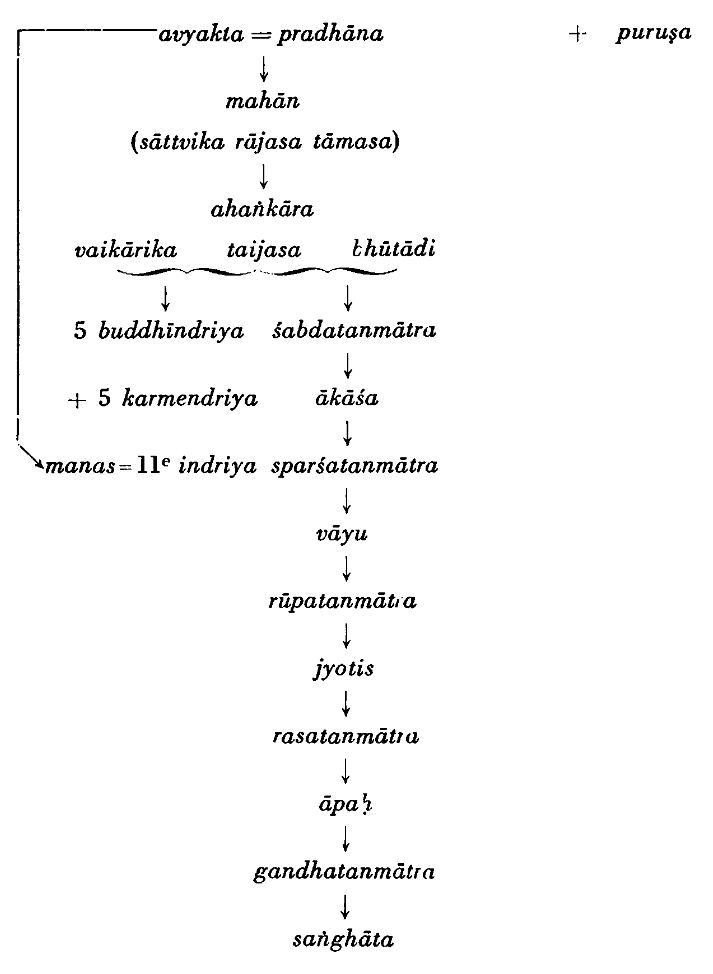
\includegraphics[height=\textheight]{chapters/media/biardeau1981-p27}
                \begin{tikzpicture}[
                  node distance=0.4cm,
                  every node/.style={font=\itshape},
                  box/.style={align=center}
                  ]
                  
                  % Top nodes
                  \node (avyakta) {avyakta = pradhāna};
                  \node[right=3cm of avyakta] (purusa) {+ \; \textit{puruṣa}};
                  
                  % Main vertical line
                  \node[below=of avyakta] (mahan) {mahān};
                  \node[below=of mahan] (gunas) {(sāttvika \; rājasa \; tāmasa)};
                  \node[below=of gunas] (ahamkara) {ahaṅkāra};
                  
                  % Threefold division with extra spacing
                  \node[below left=1cm and 2.5cm of ahamkara] (vaikarika) 
                  {vaikārika};
                  \node[below=1cm of ahamkara] (taijasa) {taijasa};
                  \node[below right=1cm and 2.5cm of ahamkara] (bhutadi) 
                  {bhūtādi};
                  
                  % Wavy brace under the three nodes
                  \draw[decorate, decoration={snake, amplitude=1mm, segment 
                      length=6mm}]
                  ([yshift=-3mm]vaikarika.south west) -- ([yshift=-3mm]bhutadi.south 
                  east);
                  
                  % From vaikārika
                  \node[below=of vaikarika] (dummy1) {};
                  \node[below=1.7cm of vaikarika] (buddhi) {5 buddhīndriya};
                  \node[below=of buddhi] (karmendriya) {+ 5 karmendriya};
                  \node[below=of karmendriya] (manas) {manas = 
                  11\textsuperscript{e} 
                      indriya};
                  
                  % From taijasa
                
                    \node[below right=1.2cm  and .5cm of taijasa] (sabda) 
                  {śabdatanmātra};
                      \node[above=of sabda] (dummy2) {};
                  \node[below=of sabda] (akasa) {ākāśa};
                  \node[below=of akasa] (sparsa) {sparśatanmātra};
                  \node[below=of sparsa] (vayu) {vāyu};
                  \node[below=of vayu] (rupa) {rūpatanmātra};
                  \node[below=of rupa] (jyotis) {jyotis};
                  \node[below=of jyotis] (rasa) {rasatanmātra};
                  \node[below=of rasa] (apas) {āpaḥ};
                  \node[below=of apas] (gandha) {gandhatanmātra};
                  \node[below=of gandha] (sanghata) {saṅghāta};
                  
                  % Connections
                  \draw[->] (avyakta) -- (mahan);
                  \draw[->] (mahan) -- (gunas);
                  \draw[->] (gunas) -- (ahamkara);
                  
                  % Branches
%                  \draw[->] (ahamkara) -- (vaikarika);
%                  \draw[->] (ahamkara) -- (taijasa);
%                  \draw[->] (ahamkara) -- (bhutadi);
                  
                  % Left branch
                  \draw[->] (dummy1) -- (buddhi);
                  \draw[->] (buddhi) -- (karmendriya);
                  \draw[->] (karmendriya) -- (manas);
                  
                  % Diagonal slanted connection back into middle branch
                  %\draw[->] (manas.east) .. controls +(3,0) and +(-3,0) .. 
                  %(sparsa.west);
                  
                  % Middle branch
                  \draw[->] (dummy2) -- (sabda);
                  \draw[->] (sabda) -- (akasa);
                  \draw[->] (akasa) -- (sparsa);
                  \draw[->] (sparsa) -- (vayu);
                  \draw[->] (vayu) -- (rupa);
                  \draw[->] (rupa) -- (jyotis);
                  \draw[->] (jyotis) -- (rasa);
                  \draw[->] (rasa) -- (apas);
                  \draw[->] (apas) -- (gandha);
                  \draw[->] (gandha) -- (sanghata);
                  
              \end{tikzpicture}
              
                \caption{Levels of original creation as presented in the following 
                Purāṇas: \emph{Vāyupurāṇa}, \emph{Brahmāṇḍapurāṇa}, 
                \emph{Viṣṇupurāṇa}, \emph{Mārkaṇḍeyapurāṇa}, 
                and \emph{Kūrmapurāṇa}, \citep[after][27]{biar-1981}. 
                See footnote \ref{puraniccosmology}}
                \label{fig:biardeau1981-p27}
            \end{figure}
            
          
            
            
            From that mutable Ahaṅkāra the 
            eleven \se{indriya}{faculties} arise, with the very same
            characteristics. It is as follows: ear, skin, eye, tongue, nose,
            speech, hand, genitals, anus, feet and mind.  Amongst these, the first 
            five are the faculties of \se{buddhi}{cognition}; the next five are the 
            faculties of \se{karma}{action}.  The mind has properties of both.
            
            From the Ahaṅkāra as \se{bhūtādi}{starting point for the
    elements}, arise the five \se{tanmātra}{bare entities},
with exactly the same characteristics.\footnote{Earlier,
    the Ahaṅkāra was said to have three aspects, so we would
    here expect a description of the \se{taijasa}{fiery}
    aspect.  But the Nepalese version goes straight to the
    \se{bhūtādi}{elemental} aspect.  The vulgate text inserts
    the fiery aspect alongside the elemental as if it were
    similar in all respects (\dev{taijasasahāya}).}  It is as
    follows: bare sound, bare touch, bare form, bare taste,
    bare smell.\footnote{Or, ``the essence of sound,'' etc.}
    
    From these \se{bhūta}{elements} come space, air, fire, water and earth; 
    from these come sound, touch, form, taste and smell, with the same 
    distinctions.  In this way these twenty-four \sepl{tattva}{principle} have 
    been explained. 
            
\item[5]    

In this context, sound and so on are the objects of the \se{indriya}{faculties} of 
cognition.  Amongst the faculties of action, they are: speaking, holding, 
enjoyment, excretion and walking respectively.  

\item[6]

The eight \se{prakṛti}{productive principles} are 
the \se{avyakta}{unmanifest},
\se{mahān}{The Great}, 
the \se{ahaṅkāra}{I-principle}, 
and the five \se{tanmātra}{fine elements}.
The rest are the sixteen \se{vikāra}{modifications}.
    
\item[7]   

Each and every one of them has a sovereign with respect to their
domain.  There is their own \se{adhyātmika}{personal aspect} and the
\se{adhidaiva}{divine aspect}. Thus, \\
\begin{center}
\begin{tabular}{ll}
\toprule
\emph{Divine} & \emph{Personal}\\
\midrule
    Brahmā & of Buddhi,\\
Īśvara &of ahaṃkāra,\\
the moon &of mind,\\
the ear &of the directions,\\
wind &of the skin,\\
the sun & of the eyes,\\
the waters &of the tongue,\\
the earth &of the nose,\\
fire &of the voice,\\
Indra & of the hands,\\
Viṣṇu &of the feet,\\
Mitra & of the anus,\\
and Prajāpati &of the genitals7.\\
\bottomrule
\end{tabular}
\end{center}
%Brahmā of Buddhi,
%Īśvara of ahaṃkāra,
%the moon of mind,
%the ear of the directions,
%wind of the skin,
%the sun for the eyes,
%the waters for the tongue,
%the earth for the nose,
%fire for the voice,
%Indra for the hands,
%Viṣṇu for the feet,
%Mitra for the anus,
%and Prajāpati for the penis.


% everything except the mahābhūtas and tanmātras - CB







\end{translation}
 % with Jan Gerris
        % !TeX root = incremental_SS_Translation.tex

\chapter{Śārīrasthāna 2:  On Semen and Menstrual Fluid}

% Jane Allred

\section{Literature} 

Meulenbeld offered an annotated overview of this chapter and a
bibliography of earlier scholarship to
2002.\fvolcite{IA}[244--246]{meul-hist}  \citet[chs 6--8]{das-2003} also
studied topics of this chapter and in chapter 13 provided an overview of
the conceptual background of ayurveda on the topics discussed in this
chapter.  

\section{Translation}

\begin{translation}
    
    \item [1] 
    
    We shall now explain The Anatomy that is the purification of 
    \saneng{śukra}{sperm} and 
    \saneng{śoṇita}{blood}.
%    \q{JG in the light of your reflections, I removed 
%    “women's fertile”. I've put śārīram back in.}
%    
    
    \item [3]  \saneng{retas}{Semen}\footnote{The Nepalese version has
    \dev{-retāṃsi} “semen” (in the plural) as the subject of the
    sentence: “seeds are unable to produce offspring\ldots.”  In the
    vulgate, \dev{-retasaḥ} is a masculine bahuvrīhi, making “men
    whose semen has\ldots” the subject of the sentence.} is
    incompetent to produce offspring if it is [characterized by] wind,
    bile, phlegm, \saneng{śoṇita}{blood},\footnote{Note that the list
        begins with the four entities, wind, bile, phlegm and blood,
        hinting at a four-humour system \citep[see][485--486]{wuja-2000}.}
        \saneng{kuṇapa}{decomposition},
        \saneng{granthi}{clumps},\footnote{\label{granthi}Modern
            Establishment Medicine (MEM) understands that normal ejaculate
            contains coagula which, however, dissolve after about half an
            hour.  But coagula that do not dissolve may sometimes be a sign of
            an underlying disorder (see, e.g., 
            \volcite{2}[614--615]{lamm-1990}; \cite{cohe-1990}).}
            \saneng{pūtipūya}{stinking pus}, \saneng{kṣīṇa}{low volume},
            urine, or feces.
    
 \subsection{Diagnosis by humours}

 \item[4]
 
 \begin{itemize}
     \item  When the dysfunction is caused by wind, there is a colour
and a type of pain that typically goes with wind problems. \item
If  caused by bile the colour and the pain are typical of bile
afflictions.  If caused by phlegm the discolouration and
suffering are characteristic for phlegm disease. \item And if
caused by \saneng{śoṇita}{blood} there will be a colouration due
to blood and a sensation of a bile affliction. Moreover, when
caused by \saneng{rakta}{blood} there is the \se{kuṇapa}{smell of
    decomposition}.\footnote{Note that the text mentions both
    \dev{śoṇita} and \dev{rakta}.  This raises the question of
    whether the author considered these to be different, or whether
    it is an artefact of textual transmission.}  \item Phlegm with
    wind causes the appearance of clumps. \item   Bile with
    \saneng{śoṇita}{blood}  causes the appearance of
    \saneng{pūtipūya}{foul-smelling pus}. \item    Bile with
    \se{māruta}{wind} cause a weakening of semen. \item      
    \se{sannipāta}{Humoral colligation} causes the smell of urine and
    feces.\footnote{The expression “humoral colligation,” translating
        \dev{sannipāta}, refers to the simultaneous disorder of three
        humours at the same time, a condition that is difficult to treat
        \citep[see][38 \emph{et passim}]{wuja-2016}.}
         \end{itemize}     
Cases of foul-smelling sperm, sperm with clumps, and when it reeks of
pus are hard to treat.  But when sperm contains urine or faeces there is no
treatment\sse{asādhya}{incurable}.\footnote{Note that the above
    characterizations presuppose the direct inspection of an ejaculate. 
    The process of collection is not described in the sources in this
    chapter.}
 
 \item[5]
 
 Moreover, \se{ārtava}{seasonal blood} too can become
\se{upasṛṣṭa}{afflicted}, \se{abīja}{seedless} because of the three
humours, and blood as the fourth, taken individually, in pairs or
triples or all together.\footnote{This translates the text of the oldest
    surviving witness, N, and the vulgate.  But MS H, that normally follows
    K very closely, has a negative particle, \dev{na}, reversing the sense
    of the sentence.}
 
 This can also be known by means of the humour, colour and pain.
 
 In these cases, that which displays \se{kuṇapa}{decomposition}, clumps 
 and the putrid smell of pus is \se{asādhya}{incurable}. And otherwise it is 
 \se{sādhya}{curable}.
 
 
%  %
%   Rather it is  the pain 
%  caused or the discoloration of the sperm itself that suggest one of these 
%  afflictions. 
  Among these, the kind which shows decomposition, or coagula, or 
  putrid pus is incurable. The other types, however, can be treated.  
 
 \item[6]
 
 And there is a verse on this. 
 
 \begin{quote}
      An expert should overcome the first three of these sperm
\sse{doṣa}{pathology}pathologies with special
treatments\sse{kriyā}{treatment} such as unction and sweating,
as well as by means of a \se{uttarabasti}{urethral
    instillation}\sse{basti}{instillation}.\label{uttarabastyantam}%
\footnote{\Dalhana{3.2.6}{345} noted that “unction and sweating”
    indicates the “five treatements”: \dev{vamana, virecana, anirūha,
    anuvāsana} and \dev{uttarabasti}.  He noted that the explicit mention
    of urethral enema in the verse was for the purpose of highlighting its
    priority. However, a natural reading of the verse does not suggest
    that these distinctions were in the author's mind.}\q{find out about
        uttarabasti}
    
 \end{quote}
 
 \subsubsection{Therapies for sperm, by humour}
 
 \item[6.1] 
 
In that context, when the sperm is of the nature of wind, there is an
\se{āsthāpana}{enema} consisting of \gls{bilva}, \gls{vidārī} and
milk.\footnote{These three recipes are not present in the vulgate text
    of the \SS.} %
    In the \sse{uttarabasti}{urethral instillation}urethral
    instillations one should use sesame oil well cooked with \gls{madhūka},
    \gls{rāsnā}, \gls{devadāru}, and \gls{sarala}. One can also make
    the patient drink clarified butter with ripe \gls{dāḍima},
    \gls{mātuluṅga} fruit, \gls{saindhava}, a \saneng{kṣāra}{caustic},
    and \gls{vasukavasira}.\footnote{\dev{-vipakva} “well cooked with\ldots” 
    might be interpreted as “with ripe\ldots”.}
 
 \item[6.2]
 
 When the sperm is of the nature of bile, there is  an
\sse{āsthāpana}{enema}enema of milk cooked with curds, \gls{śrīparṇī}
and \gls{madhuka}k. %
One should also apply a \se{kalka}{paste} of \gls{sarja} and
\gls{dhava} in the vagina. %
There is an \se{anuvāsana}{oily enema} of sesame oil cooked with
\gls{madhuka}; in the same way, it should only be applied as a
urethral instillation.\footnote{By specifying “upper (i.e., urethral) instillation”
    the author is clarifying that this is not a rectal enema.}

  One should make him swallow ghee cooked with 
  \gls{kāṇḍekṣu},
  \gls{śvadaṃśtra},
  \gls{guḍūcī},
  \gls{madhuparṇī},
  \gls{bhṛṅga},
  and 
  the \gls{pañcamūla}.
  
 \item[6.3]
 
When the sperm is of the nature of phlegm, there is  an
\se{āsthāpana}{enema} consisting of a \se{kaṣāya}{decoction}  of
\gls{rājavṛkṣa}.  And one should also apply an \se{anuvāsana}{oily
    enema} of sesame oil cooked with \gls{pippalī}, \gls{viḍaṅga} and
honey; and it should only be applied as a urethral instillation. 

One should make him drink a ghee cooked with 
\gls{pāṣāṇabheda},
\gls{kāśmaryā},
\gls{āmalaka},
\gls{pippalī},
\gls{vasuka}, and 
\gls{vasira}.
 
 
\item [7]
 
  And there are verses about this:
 
 \begin{quote}
     When there is blood in the sperm, the physician should give the person ghee 
 cooked with 
 flowers of the \gls{dhātakī},
 \gls{khadira},
 \gls{dāḍima},
 and \gls{arjuna}.
 \end{quote}
 
 \item [8]
 
\begin{quote}
     When it smells like a corpse, he should drink ghee cooked with
the \gls{śālasārādi}. %
\dag When clumps appear, it is cooked with stones, or also in ash from
a \gls{palāśa}.\footnote{The Nepalese text and translation of this
    sentence are uncertain. The vulgate text reads, \Su{3.2.8}{345}:
    \dev{granthibhūte śaṭīsiddhaṃ pālāśe vā 'pi bhasmani} “If clumps
    appear, it is cooked with \emph{śaṭī} or in ash from a \emph{palāśa}.”
    The vulgate edition notes in a footnote that some vulgate manuscripts
    add an extra line, \dev{snehādiśca kramaḥ ṣaṭsvetāsu vijānatā}. The
    Nepalese manuscripts read this line two verses further down.}
\end{quote}

 \item[9]
 
\begin{quote}
    And also, when it resembles pus, it is treated with items such as
\gls{parūṣaka} and \gls{vaṭa}.  When the sperm is deficient it should be
treated as was stated before and also as will be
described.\footnote{\Dalhana{3.2.9}{345} noted that “what was stated
    before” refers to the \dev{svayonivardhana} section, i.e., \SS\
    \Su{1.15.10}{69}, and that “what will be described” refers to \SS\
    \Su{4.26}{496}, the chapter on weakness and strength
    (\dev{kṣīṇabalīya}).}
\end{quote}
 
 \item [10]
 
 \begin{quote}
     When it looks like feces, he should be made to drink ghee together with
\gls{citraka}, \gls{uśīra} and \gls{hiṅgu}.
 \end{quote}

 
\item[10.add1] 

\begin{quote}
    In these six cases, a wise person should carry out the sequence that
starts with oleation.\footnote{It is uncertain which six cases 
    the author intended, but probably it refers to the behaviours
    listed in the next verse.}
\end{quote}

\item[10.add2--3] 

\begin{quote}
It deteriorates as a result of not having sex with women for a long
time as well as from the use of actions, and from overusing the drugs
that are astringent, spicy and sharp, that are \se{amla}{acidic},
salty, \se{rūkṣa}{sere}, \se{śukta}{sour} or \se{paryuṣita}{stale},
and because of \se{vegāghāta}{suppressing} the impulses in vaginas and
from \se{gamana}{intercourse}.\footnote{This passage is hard to
    interpret and there are no parallels, commentary or meaningful
    alternate readings.}
\end{quote}
   
\subsection{Therapies for menstrual blood} 
  
\item[10.add4]

\begin{quote}   
   When there is a \se{doṣa}{defect} in the \se{ārtava}{menstrual blood}
   one should advise the therapy starting with oleation.
   
   And one should use a \se{uttaravasti}{urethral instillation} exactly as was 
   described before.
   \end{quote}
%
%
\item[10.add5]\q{Add tr.\ of 3.2.10.add5--3.2.10.add11}
\item[10.add6]
\item[10.add7]
\item[10.add8]
\item[10.add9]
\item[10.add10]
\item[10.add11]
%
%

   \item [12cd]
   
And there is a verse about this:
\begin{quote}
     To purify the \se{ārtava}{menstrual blood}, one should apply the procedure 
    that finishes with a \se{uttarabasti}{urethral instillation}\footnote{The
        “procedure ending with a urethral instillation” probably refers to verse
        6 above (see page \pageref{uttarabastyantam}).}
\end{quote}   
    
 \item[13cd]  
 
 One should use a \se{kalka}{paste} as well as cloths and a salutary
\se{ācamana}{lavages}.\footnote{The word \dev{ācamana}, normally
    “sipping water from the palm” is here translated “lavage” following the
    context and \Dalhana{3.2.13}{345}, who described it as “water for
    washing the vagina” (\dev{yoniprakṣālanodaka}).  This treatment may be
    intended for the condition mentioned in 12cd, but in the vulgate text
    there is a preceding half verse stating that the treatment is for the
    “four disorders of menstrual blood.”}
    
\item[14cd]

In case of a bad smell and the appearance of pus, or the appearance of
marrow in the blood.

\item [15]
\label{3.2.15}

She should drink a \se{kvātha}{decoction} of \gls{bhadraśrī} or a
decoction of red \gls{candana}.\footnote{The name \dev{candana} may
    refer to several types of sandalwood; presumably one is meant here
    that is different from white sandalwood, i.e., perhaps Pterocarpus
    santalinus Linn.\ f.  The vulgate has an extra half-śloka here.}
 
\item[14ab]
 
 When \se{granthi}{clumps} appear, she should drink \gls{pāṭhā}, 
 \gls{tryūṣaṇa}, and \gls{vṛkṣaka}.\footnote{On \dev{granthi}, see note 
 \ref{granthi}.}
 
 \item[14.add1] 
 
 She should drink a a \se{niḥkvātha}{decoction} that is the
\se{surasa}{extracted juice} of  a \se{kṣāra}{caustic}, \gls{nāgara},
and \gls{hiṅgu}.\footnote{At this point, the sequence of passages in the 
Nepalese version differs substantially from the vulgate.  For example, the next 
passage in the vulgate, 3.2.15, occurs above, and the next below on 
p.\,\pageref{3.2.15}.}
 
\item[24]

Thus a man has unblemished semen and a woman has pure menstrual 
blood.\footnote{On this and the following texts, cf.\ \cite[389 et 
passim]{smet-2010}.}
 
 \subsection{During menstruation}
 
 \item[25]
 \label{3.2.25}
During the \se{ṛtu}{season}, starting from the first day onwards, the
\se{brahmacāriṇī}{chaste woman} foregoes bathing, anointments,
ornaments and \se{vilekhana}{grooming}.\footnote{The word \dev{ṛtu}
    “season” in āyurvedic texts can, according to context, refer either to
    the period of menstruation or else to the period of fecundity
    following menstruation \citep[15\,ff., note 27, \emph{et
    passim}]{das-2003}. \Dalhana{3.2.25}{347} noted that the woman's
    abstention should last three days from the first appearence of her
    menses.} She should abstain from sleeping during the day, collyriums,
    \se{aśrupāta}{weeping tears}, massages, cutting her nails, taking
    showers, laughing, telling stories, hearing too much noise and from
    exertion.\footnote{On the similar prohibitions relating to a
        menstruating woman as described in Dharmaśāstra literature, as well as
        the similar defects accruing from disobedience         
        \citep[see][284--287]{lesl-1989}.}
        
For what reason?  By sleeping during the day, the fetus becomes
\diff{deaf}.\footnote{Here, the vulgate reads \dev{svapnaśīlaḥ} “he
    tends to sleep.”} From collyrium he becomes blind.  From weeping, his
    vision is impaired. From bathing and anointing, he becomes badly
    behaved. From massage with oil he gets a \se{kuṣṭha}{pallid skin
        disease}.\footnote{On translating \dev{kuṣṭha} in Āyurvedic texts, see
        \cite[96\,ff]{emme-1984}.} From cutting the nails he gets
        \se{kunakha}{ugly nails}.  From smearing an unguent he becomes bald.
        From habitually exercising in the open air he goes mad. For this
        reason one should avoid these.
    
For three days of ritual food, the husband should \se{\root rakṣ}{protect} the
woman.  She lies on a layer of \gls{darbha}, and eats a different kind of food
from the palm of her hand, or from a plate or from a leaf.\footnote{This
    sentence is hard to construe because \dev{haviṣyaṃ} “ritual food” cannot 
    agree
    with \dev{-bhojinīṃ}.}

On the forth day, one should  show to the husband the woman 
who has
had a purifying bath, is wearing unstitched clothes, is ornamented and who has
chanted a benediction and recited a blessing.\footnote{See \cite[58 and
    fn.\,167]{wuja-2023}.}
    
    What is the reason for that?
     
     
     \item[26]
     And there is a verse on this.
     
     \begin{quote}
         
         A woman has a bath after her period.  The type of man she sees after 
         that determines the type of son to whom she will give birth. She may then 
         show her son to her husband.     
           
     \end{quote}
        
        \item[27]
        
\begin{quote}
            Next, the \se{upādhyāya}{priest} should perform the appropriate 
            ritual 
        for producing a son.  At the end of the ritual, the \se{vicakṣaṇa}{expert} 
        should anticipate the following procedure. 
 
\end{quote}       

\item [28] Next, after the man has eaten a rice porridge with ghee and
milk in the afternoon, having been celibate for a month, at night he
should sexually approach the woman who has had a diet rich in oil and
mung beans.  He then soothes her in a friendly way and he may go to
her optionally on the fourth, sixth, eighth, tenth or twelfth
day.\footnote{In the Nepalese version, this text presents a general
    rule for lovemaking on even days.  In the vulgate, the word
    \dev{putrakāma} is added, making this a specific rule for conceiving a
    male child.  After this text, sections 29, 30 and 31 of the vulgate
    are not present in the Nepalese version.  These verses state that the
    above-mentioned special days are beneficial, that odd days lead to the 
    conception of a girl child, and finally the vulgate gives a list of the 
    consequences of conceiving a child with a menstruating woman.}
        
\q{29, 30 missing?}
        
 \item [31]

Henceforth, he should approach after a month

[At this point there is a misplaced folio in MS N]
  
\item[32] 

\textcolor{red}{And when conception has occurred in this 
way}\q{\textcolor{red}{Problematic 
passage in the edition.}}

During one of these nights, the pregnant woman should press three or
four drops of juice from one or other of the following:
\gls{lakṣmaṇā}, \gls{vaṭa}, \gls{śuṅgā}, \gls{sahadevā},
\gls{viśvadevā}. Then she should administer them in the right nostril if she
desires a son and in the left if she wants a girl, and she should not
sneeze them out.\footnote{There is a textual problem at the start of this 
passage.}




\item[33]

\begin{quote}
    For certain, in the presence of these four, a fetus that follows
the rules will come into being, just like a sprout is from a
combination of field, seed, water and grass.\footnote{The Nepalese
    version reads \dev{kṣettrabījodakatṛṇām} “of field, seed, water
    and grass” in contrast to the vulgate's \dev{ṛtukṣetrāmubījānām}
    “of season, field, water and seed.” This gives the two versions
    quite different meanings. In the Nepalese version, the author is
    referring to the four plants mentioned in the previous verse,
    \gls{lakṣmaṇā}, \gls{vaṭa}, \gls{śuṅgā}, \gls{sahadevā}, and
    \gls{viśvadevā}.  Then the author presents a simple agricultural
    simile.  In the vulgate version, the words of the compound each
    have a double meaning: they can refer to the agricultural simile,
    but they can also be construed to mean “menstrual season, womb,
    nourishing bodily fluids, and male and female semen,” a
    parallelism not present in the Nepalese transmission.   This is
    how Ḍalhaṇa interpreted the verse.}
\end{quote}

\item[34] 

Children born in this manner are beautiful, of noble character and
enjoy long lives.\footnote{We translate \dev{mahāsattvāḥ} as “noble
    character;” Ḍalhaṇa, commenting on the vulgate reading
    \dev{sattvavantaḥ}, refers to the \dev{guṇas}, interpreting the
    expression as “not strongly influenced by \dev{rajas} and
    \dev{tamas}.”}  They provide release from \se{ṛṇa}{obligation} and
    they themselves have children, benefitting their parents.\footnote{Children 
    born in this manner
        fulfil their parent's obligation to have children and they themselves
        have children, thus continuing the family.  The three debts are
        normally understood as being to the gods, the ancestors and to sages.
        But Ḍalhaṇa's phrasing is odd in that he says
        \dev{pitṝṇāmṛṇatrayamokṣaṇaśīlāḥ} “behaving so as to provide release
        from the three debts to the ancestors.”} 

\item[35]

In that context, the element of \se{tejas}{heat} is the most important
factor as far as \se{varṇa}{complexion} is concerned. That being
granted, at the moment the fetus is formed, when the food has water as
its chief element, then the fetus is fair.\footnote{The food of the
    mother, that is.}  When earth is the predominant element, it is
    \se{kṛṣṇa}{dark}. When earth and ether are the chief elements, it is
    \se{śyāma}{dark brown}.\footnote{The terms \dev{kṛṣṇa} and \dev{śyāma}
        often mean more or less the same, a dark blue or black colour. The
        latter can shade into brown or dark green.}  Some people say that the
        \se{prasava}{newborn} has the same colour as the colour of the food
        that the pregnant woman commonly eats. Similarly, creatures like
        snakes, scorpions and \glspl{galagoḍikā} that inhabit black, yellow or
        white habitats are black, yellow or
        white.\footnote{\label{galagodika}Cf.\ also n.\,\ref{godheraka},
            p.\,\pageref{godheraka}. Cf.\ \volcite{IA}[70 and notes]{meul-hist} on
            these poisonous animals as described in the \CS, and
            \cite[455-456]{meul-1974} on the names \emph{kṛkalāsa\slash
            kṛkalāśaka, śaya} and \emph{saraṭa} and the confusion surrounding this
            topic and the indigenous names of some species such as \emph{ṭikṭikī,
            jyeṣṭhi, jyaiṣṭhī}, \emph{girgiṭ}.}
            
In that context, \se{jātyandha}{congenital blindness} is caused by
the element of \se{tejas}{brilliance} not reaching the location of
\se{dṛṣṭi}{eye}.  Similarly, red eyes are a consequence of blood,
white eyes are a consequence of phlegm, yellow eyes are a consequence
of bile, and \se{vikṛtākṣa}{dysfunctional eyes} are a consequence of
wind.\footnote{The term \dev{vikṛtākṣa} was known to Kātyāyana
    (\emph{Mahābhāṣya} on P.6.3.3, \pvolcite{3}[142]{kiel-1880}).}
  
% got to here 2024-06-14 


\item[35.1--4]

And on this, there are the following:\footnote{The next four verses are 
absent in the vulgate; they were reproduced by the 
editor in a footnote (\cite[348a, n.\,3]{vulgate}).

The phrase “and here are some verses” appears 
in the vulgate before 3.2.36.}

\begin{quote}
    %1
If a pure wind affects someone's eyes, they become
sunken, blue and dark.

% got to here 2024-08-30
    
    %2
When bile mixed with phlegm, with no impurity, goes into
someone's eyes, their eyes are termed “yellowish-red.”
    
    %3
When phlegm that is free of any impurity moves to the eyes, their
eyes shine with a white circle within a circle.\footnote{Perhaps this
    describes the appearance of arcus senilis.}
    
    %4
When blood mixed with phlegm moves into the eyes, those people
have eyes that become pigeon-blue, or else bloodshot.
  
    \end{quote}

\item [36]

Just as the ghee in a pot placed on a fire melts, so the menstrual
blood of a woman may flow out after sex with a man.\footnote{It is
    difficult to know what the author means here, since menstruation is
    not physiologically caused by intercourse.
    
Note that the text actually says “a pot of ghee \ldots\ melts.”  But it's
not the pot that melts, but the ghee.  This may explain the vulgate
reading \dev{ghṛtapiṇḍa} “a lump of ghee.”  The reviser did not like
the imprecise idea of a pot melting.}

\item [37]

But when the wind splits the \se{bīja}{seed}, two lives 
(\emph{jīva})\sse{jīva}{life} come into the \se{kukṣi}{belly}.
They are called “\se{yama}{twins},” being created from preceding
\se{dharma}{virtue} or its opposite.\footnote{Note the adverbial 
\dev{-purā} at the end of a Bahuvrīhi.  

The commentator Gayadāsa (cited here by Ḍalhaṇa) disagreed with this
interpretation.  He preferred to understand \dev{dharmettara} not as
“dharma and its opposite,” but as “the opposite of dharma.” He
explained that according to both scripture and tradition, twins are
the result of \dev{adharma} “sin,” and that is why penances are
necessary after the birth of twins (on \Su{3.2.27}{348}).

The next two verses are absent in the vulgate; they were reproduced by the 
editor in a footnote (\cite[348b, n.\,3]{vulgate}).}

\item [37.1]
\begin{quote}
    When the mixing is happening, if the man's \se{retas}{semen} is plentiful 
    and pure then the pregnant woman gives birth to two boys.
\end{quote}

\item [37.2]

\begin{quote}
    When the mixing is happening, if the woman has a lot of 
    \se{śukra}{semen} then the pregnant woman gives birth to two girls.
    There is no doubt about this. 
\end{quote}

\subsection{Types of persons}

\item[38]

The term for men and women who have diminished seed is
\emph{Āsekya}\sse{āsekya}{having diminished
    seed}.\footnote{Etymologically, “to be poured into."  On this and the
    following typologies, see the brief treatment by
    \citet[216--217]{meul-1997}.}  Without doubt, after eating something
    \se{śukla}{white}, his flag is raised.\footnote{\Dalhana{3.2.38}{348}
        made it clear that this is a metaphor for having a penile
        erection.\label{erection}

“Eating something white” may refer to \dev{śukra} “sperm,” as the
vulgate reads.  But note that works on aphrodisiacs and fertility
(\dev{vājīkaraṇa}) in āyurveda and rasaśāstra routinely recommend
white substances such as milk for strengthening reproductive ability.
See, for example, \SS\ \Su{4.26.27--31ab}{498} and \CS\ \Ca{6.2, all of
sub-chapter 2}{392--394}.

The vulgate has a different reading for the first half of this verse, stating that 
such a man is a product of parents with deficient seed.  Ḍalhaṇa also gave a 
detailed description of a man eating the semen ejaculated by another man, 
and he stated that the terms \dev{ṣaṇḍa} and \dev{mukhayoni} were 
synonyms for such a person.

The term \dev{āsekya} is given in \cite[161]{moni-sans} as “impotent,
a man of slight generative power.”  This is wrong.  It is the
referent of the term, not its meaning. Cf.\ \volcite{1}[98]{josi-maha}.

\label{ṣaṇḍha}
Some of the features referred to by the term \dev{ṣaṇḍa/ṣaṇḍha} may
have included conditions today covered by
Mayer-Rokitansky-Küster-Hauser syndrome and Morris syndrome.  The
central idea in the Sanskrit usages was that such a person cannot
produce children.}

\item[39]

Someone who is born in a foul womb is termed a \emph{Saugandhika}. 
That person gains strength from smelling a vagina and a
penis.\footnote{Etymologically, “Sweet Smelling."}

\item[40abc]

A man, who has activity in his own anus because of being celibate and
then has activity amongst his own women is known as a
\emph{Kumbhīka}.\footnote{The vulgate adds an avagraha before
    \dev{brahmacaryād}, meaning “because of \emph{not} being celibate."
    \Dalhana{3.2.40abc}{348--349} read the text this way, paraphrasing
    \dev{abrahmacaryāt}, thus inverting the meaning but not clarifying
    what he thought it meant.  But he then cited a passage from “others”
    that read \dev{brahmacaryāt}, i.e., the anal sex followed or was
    caused by celibacy, \dev{brahmacaryāt
    klaibyavaśasaṃjātāpravṛttitvāt} “because of celibacy, that is,
    because of being unable to perform because of the effect of
    impotence."  These unnamed commentators also referred explicitly to
    erectile dysfunction, \dev{śithilenaiva mehanena}, as the result of
    this celibacy and proposed that a man could get an erection through
    abnormal (\dev{viprakṛtyā}) means and as a result could have sex as a
    male with a woman.  Ḍalhaṇa also stated that the origin of a person
    with such a condition was described “in another book”
    (\dev{tantrāntare}), and proceeded to cite \CS\ \Ca{4.2.20}{303}.  
    Ḍalhaṇa then also cited another verse from Gayadāsa, who himself 
    ascribed it to Kāśyapa \pvolcite{IA}[164--166]{meul-hist}, saying that, “A 
    Kumbhila (\emph{sic}) is born when a man with phlegm for semen 
    has sex with a woman who is not passionate (or not menstruating) during 
    her season, when the love is attached to another.” (Also cited in 
    \volcite{1}[220a--b]{josi-maha}.)
    
    It is noteworthy that the \SS\ is factual and descriptive in
these passages, as befits a medical work, while the commentators
introduce a moralistic and critical tone.}

\item[40d--41abc]

Hear about the next one, the \emph{Īrṣyaka}.  
Someone who has sexual activity after seeing the copulation of other people 
is termed an Īrṣyaka.\footnote{Etymologically “one who envies."  
    
    Here again, \Dalhana{3.2.40--41}{349} cited the opinion of “another 
    book” and cited a passage from \CS\ \Ca{4.2.20}{303} that covers similar 
    ground.  The description of the \CS\ is causally framed in terms of the 
    factors \dev{vāyu} and \dev{agni}.} 

\item [41d--42]

Hear about the fifth, the \emph{Ṣaṇdhaka}.  A man who, out of
delusion, has sexual activity with a \se{kaumārī}{young girl} during
her season as if he were a woman.  In such a case, a male is born who
looks and behaves like a woman.  He is termed a
\emph{Ṣaṇḍha}.\footnote{The vulgate's \dev{bhāryā} “woman, wife” for
the Nepalese version's   \dev{kaumārī} “girl” is probably bowdlerization.}
    
\item[43]
    
Moreover, if a woman, during her season, has sexual activity like a man, then 
if a girl is born she will have the behaviours of a man.

\item[44]

The \emph{Āsekya}, the \emph{Sugandhin}, the \emph{Kumbhīka} and the
\emph{Īrṣyaka} are known to have semen.  The man with no semen is
termed a \emph{Ṣaṇḍha}\sse{ṣaṇḍha}{a man with no semen}.\footnote{It
    remains a question as to whether the authors meant the absence of an
    ejaculate or the clinical observation of childlessness even in the
    presence of an ejaculate. For a discussion of the present passages and
    further literature on \dev{ṣaṇḍha}, see \cite[581--584]{das-2003}; on
    \dev{āsekya}, see ibid., 527.  See also \cites[593--597, et
    passim]{swee-1993}{zwil-2000}{zwil-2010}.}
    
\item [45]

In both of these cases, they have a semen-carrying vessel that
dilates as a result of unnatural
excitement.\footnote{\Dalhana{3.5.45}{349} %pointed out that a Ṣaṇḍha
    % has just been defined as not having an ejaculate,
    % so why are we talking about them having semen-carrying tubes.
    cited the expression \dev{naranārīṣaṇḍhau} from the \CS\
    (Ca{4.2.17}{303}, reads \dev{-nāri}) to establish that women too may
    have these unnatural excitements.
    
    We have emended
    the Nepalese verb to the singular, because witness H clearly has
    \dev{śukravahā sirā} “semen-carry vessel” in the singular. Does
    Ayurvedic anatomy have a single vessel or many? \CS\ \Ca{3.5.8}{250}
    has a plural, \dev{śukravahānāṃ srotasāṃ}.  But the \SS\
    \Su{3.9.12}{3.9.12} has a clear statement that there are two
    \se{srotas}{ducts} that carry semen: \dev{śukravahe dve tayormūlaṃ
    stanau vṛṣaṇau ca} “there are two vessels that carry semen.  They are
    rooted in the breasts and the testicles.”  The Ayurvedic Man painting
    has a single \dev{śukramārga} \citep[233, 243]{wuja-2008a}.  The
    Jaina \emph{Tandulaveyāliya} lists 10 sperm-carrying vessels
    (\dev{dasa sirāo sukkhadhāriṇīo},
    \cites[145\,ff]{schu-1969}[5]{cail-2019}; I am grateful to Jan
    Gerris for this reference).}  Then the flag may be
    raised.\footnote{On this euphemism, see footnote \ref{erection}
        above.}


\subsection{Birth irregularities}

\item[46]

The \diff{appearance}, behaviour and mentality that is associated
with a man and a woman is also the same as that which their
\diff{offspring} (\emph{garbha})\sse{garbha}{offspring} has.\footnote{The
    vulgate has “food” for the Nepalese version's \dev{ākāra}
    “appearance,” and “son” for “offspring." The Nepalese version seems more
    perceptive on this point of heredity.}

\item [47]

Whenever a woman and a woman have sex together, they release semen on 
each other. Then a being without bones comes into being.\footnote{The 
grammar of the Nepalese and vulgate versions of this verse are quite 
different.  

This striking verse has been discussed by several scholars 
\citep[e.g.,][232--233]{smet-2006}. 
The concept of a being born with flesh but no bone and vice versa occurs in 
\emph{Jaiminīyabrāhmaṇa} 1.259 and \emph{Ṣaḍviṃśabrāhmaṇa} 2.1.1  
\citep{kolh-2005} and later in Purāṇic literature \citep{doni-1980}. 

The Nepalese version of the \SS\ does not have the following two verses that 
occur in the vulgate.  \Dalhana{3.2.48--48}{349} said that Jejjaṭa did not read 
these two verses.  Thus, the Nepalese version is the same as Jejjaṭa's version, 
as far as this omission is concerned.}

\item [50]

\diff{Offspring} (\emph{garbha})\sse{garbha}{offspring} of a deformed 
shape like a gourd, a scorpion or a snake and 
others of the same type are known to be often brought about by 
sin.\footnote{The vulgate version of this text says that it is sinful behaviour of 
women that causes abnormalities.  The Nepalese version is quite different, 
simply attributing deformity to sin and not blaming women at all.}

\item [51]

Offspring that is \emph{vimānitaḥ}\q{unsolved problem} by irritation
of wind and by pregnant longing may become hunchbacked, have a
\se{kūni}{shrivelled hand}, be lame, mute or have a
stutter.\footnote{The Nepalese version has \dev{kūni} while the
    vulgate reads \dev{kuṇi}. \Dalhana{3.2.51}{349} felt the need to
    explain the unusual term, saying \dev{kuṇiḥ vikalapāṇiḥ} “having a
    crippled hand,” but \citet[footnote 5]{acar-1939} noted a variant
    \dev{vikṛtapāṇiḥ}, suggesting some instability in the interpretation
    of this term. \Cakra{8.2.21}{690} gave the meaning \dev{kubjitakaraḥ}
    “having a hunched hand” (where there is also a variant reading
    \dev{naṣṭakaraḥ}), cf.\ \volcite{1}[216]{josi-maha}.   The Tamil
    lexemes\emph{ kū\b n} means “bend, curve, hump on the back, humpback”
    and \emph{kū\b ni} means “\ldots\ become hunchbacked"
    \citep[\#1927]{DED}. It seems likely that this is a Dravidian word
    that has been absorbed into Ayurvedic terminology at an early
    period. Medically speaking, the connection of these conditions
    with pregnancy might suggest isome of the features of 
    Amniotic Band Syndrome.}
    
\item[52]

The newborn may have abnormalities because of the bad behaviour of
its mother and father and because of bad actions from the past,
by means of the irritation of wind etc.\footnote{\Dalhana{3.2.52}{349}
    took the position that the bad actions were those of the parents, not
    the child.}

\item[53]

The child in the womb does not make wind, urine and feces because it has little 
impurity and because the wind in the stomach is not functioning.

\item[54] 

The child in the womb does not cry out because the movement of the wind is 
obstructed since the mouth is covered by the caul and the throat is surrounded 
by phlegm. 

\item[55]

The inward and outward breathing, movement and sleep that the fetus adopts
conform to the  inward and outward breathing, movement and 
sleep of the mother.

\item[56]

The composition of the body parts, the descent and appearance of the
teeth, the absence of hair on the palms all happen by
themselves.\footnote{The text reads \dev{śarīrāṇām} “of the bodies”
    that we have translated “of the body parts,” following Ḍalhaṇa's
    interpretation.  He also said that “palms” included the soles of the
    feet.}

\item[57]

Those cultivated people who in previous embodiments were constantly
aware of the scriptures are rich in sattva and have
memory of their previous births.\footnote{The vulgate text adds
    a final verse about how the karma of a previous embodiment 
    follows a person to his new life.  Witness L adds yet another verse 
    that says the lack of hair on the palms is because they come from the 
    mother, while the areas of the body from the father have much hair.}
    
\bigskip

Here ends the second chapter that is the anatomy.
    
%3.2.52 
%Because of being without religious teacher and (ca) because of misfortunes 
%of 
%the parents or due to the excessiveness of the wind-eaters the child  could 
%obtain disfigurement.
%
%3.2.53 
%Due to the scantiness of bodily excretions, itself due to a disabling of Vāyu 
%with respect to processing of food, the foetus, whilst in the womb, produces 
%(almost)* no urine nor stools. 
%
%3.2.54 
%Due to the dwindling of the Vāyu in the face, the covered parts and the 
%narrowest parts (all) wrapped up by phlegm (kapha-), the foetus while it is in 
%the womb because of obstruction of the going does not weep all the time*.   
%
%3.2.55 
%Thus the foetus, provided with the movements of inhalation and of 
%exhalation, 
%goes on; the coming together of (its) moments of sleep with the movements 
%of 
%inhalation  and of exhalation of the mother.
%
%3.2.56 
%The (adjustment?) of the (limbs of the) body and both the appearance  and 
%the 
%falling of the teeth, even (ca) the very non-appearance of hairs  in the palms 
%of 
%the hands and the soles of the feet, (goes) according to its intrinsic nature ||
%
%3.2.57 
%Men who have uninterruptedly entered one previous existence after another 
%and who have a vast understanding of the scriptures, do remember their own 
%previous births.
%
%This was the second chapter of the śārīrāsthana.
%  
%\end{tt}

\end{translation}
 % with Jan Gerris
        \include{chapters/translation 3-03} % with Jan Gerris
            \thispagestyle{empty}
        
        \part{Part 4. Cikitsāsthāna}
        
        \include{chapters/translation 4-04}
            \thispagestyle{empty}
        \include{chapters/translation 4-05}
            \thispagestyle{empty}
        \include{chapters/translation 4-15}
            \thispagestyle{empty}
        
        \part{Part 5. Kalpasthāna}
       
        % !TeX root = kalpasthana-book.tex

\chapter{Kalpasthāna: Introduction}

The \emph{Kalpasthāna} of the \emph{Compendium of Suśruta} is one of
the most important treatises on toxicology surviving from the ancient
world.\footnote{\citet{liu-2021} provides a valuable overview of
    poison treatises in the ancient world, inexplicably omitting mention
    of the \emph{Kalpasthāna}.} Other treatises, such as the
    \emph{\textgreek{θηριακά}} (\emph{On Beasts}) and
    \emph{\textgreek{Ἀλεξίφαρμακα}} (\emph{Antidotes}) of Nicander of
    Colophon (fl.\ second century \BCE) or the \emph{\textgreek{Περὶ τῶν
            ἰοβολῶν θηρίων καὶ δηλητηρίων φαρμάκων}} (\emph{On Venomous 
            Beasts and
        Poisonous Drugs}) by Aelius Promotus (fl.\ ca.\ first century \BCE --
    first century \CE) do not approach the \emph{Kalpasthāna} in length,
    taxonomic detail or organization.\footnote{On Nicander, see
        \cite{gow-1953} and the facsimile of \MS{Paris BNF Greek suppl.\ 247}
        published by \citet{touw-1997}.  On Aelius Promotus, see
        \cites[29]{smit-1870}[363--368]{gost-1897}{ihm-1995}.}

%\cite{Paris-suppl-247}

\section{The Sequence of Chapters}
\label{kalpa-chapter-sequence}

The Nepalese version of the \SS\ reverses the sequence of chapters six and 
seven (see 
Table~\ref{kalpa-chapters}).


%
\begin{table}
    \centering\large
    \caption{Chapters of the \emph{Kalpasthāna}.}
    \medskip
    
% Define the column types: l for left-aligned text, c for centered numbers
\begin{tabular}{l c c}
   
    \emph{Chapter title} & \emph{Nepalese} & \emph{vulgate} \\
    \toprule
    Annapānarakṣākalpa & 1 & 1 \\
    Sthāvaraviṣavijñāna & 2 & 2 \\
    Jaṅgamaviṣavijñāna & 3 & 3 \\
    Sarppadaṣṭavijñāna & 4 & 4 \\
    Sarppadaṣṭacikitsita & 5 & 5 \\
    % Use \tikzmarknode{<name>}{<content>} to create a node around 
    %the number
    \textbf{Mūṣikākalpa} & 6\tikzmarknode{A}{} & \tikzmarknode{B}{}7 
    \\
    \textbf{Dundubhisvana} & 7\tikzmarknode{C}{} & \tikzmarknode{D}{}6 \\
    Kīṭakalpa & 8 & 8 \\
    \bottomrule
\end{tabular}
% Use TikZ to draw the lines after the table is built
\begin{tikzpicture}[overlay, remember picture]
    % Draw the first crossover line: A (Nepalese 6) to B (vulgate 7)
    % We connect the center of the nodes A and B
    \draw[->] (A.center) -- (D.center);
    
    % Draw the second crossover line: C (Nepalese 7) to D (vulgate 6)
    \draw[->] (C.center) -- (B.center);
\end{tikzpicture}


\label{kalpa-chapters}
\end{table}
%
% TODO: \usepackage{graphicx} required
%\begin{figure}
%    \centering
%    \includegraphics[width=0.65\linewidth]{chapters/media/kalpa}
%    \caption{}
%    \label{fig:kalpa}
%\end{figure}
%
\noindent
This difference in sequence does not have an immediately obvious 
significance, but it appears to be the most original known sequence of 
chapters, since it was already known to Jejjaṭa.\footnote{See note 
\ref{dalhana-rat-sequence} below.}

\section{The Spread of Indian Toxicological Lore to Medieval Islamic  
Authors}

\section{The \emph{Kalpasthāna}'s diffusion}

From the late eighth century onwards, the \emph{Kalpasthāna}, or parts
of it, began to circulate beyond the Indian subcontinent and to
influence medical literature in early Persia, Tibet and Cambodia.

In the late eighth century, the \emph{Kalpasthāna}, as part of the
\SS, was translated into Persian and Arabic at the Abbasid court of
Baghdad by an Indian physician who is often known by the name
Mankah.\footnote{On the name and its variants, see \volcite{IB}[202,
    notes 2, 3]{meul-hist}. For an account of this translation process see
    the account of \citet[14--18]{kahl-2015} and especially his useful
    reconstruction of likely historical events (16--17).}  The principle
    source of information about this translation is the \emph{ʿUyūn
        al-anbā' fī ṭabaqāt al-aṭibbā} of Ibn Abī Uṣaybiʿah
    (ca.\,1201--1270).\footnote{On Ibn ʿAbī Uṣaybʿiah, see
        \cite{hill-2019}. This author based his information on the earlier
        authors  Abū Ḥafṣ al-Kirmānī (fl.\,ca.\,800) and on an-Nadīm
        (d.\,990). Al-Kirmānī's treatise is unfortunately lost to history and
        known only through citations in other authors (see
        \cite{bosw-1994,blad-2011}).} Ibn Abī Uṣaybiʿah mentioned that al-Rāzī
        used the \SS, among other Indian works, and that it had been
        translated into Arabic at the orders of the Barmakid Yaḥyā ibn
        Khālid.\footnote{\volcite{3.2}[987]{sava-2019}. Ibn Abī Uṣaybiʿah said
            the work consisted of ten chapters, which does not match the six books
            of the known \SS.  He listed separately a work on poisonous snakes
            that could have been the \emph{Kalpasthāna} (\emph{ibid}, 989).  On
            the transmission of Sanskrit medical knowledge to Baghdad through the
            influence of the Barmakids, see
            \cites{blad-2011}{shef-2013}{kahl-2015}{wuja-2016a}.}  The \SS\
            passages used by al-Rāzī have been identified and printed in parallel
            with the Arabic translation by
            \citeauthor{kahl-2015}.\footnote{\cite[76--82]{kahl-2015}.
                Unfortunately, Kahl (p.\,14) accepted the impossible dating of a
                medical author Suśruta to the sixth century \BCE, in spite of citing
                \citeauthor{meul-hist}, \emph{HIML}, amongst his references. However,
                his remarks dating the redaction of the \SS\ to the period third-sixth
                century \CE\ are not incorrect.}
                
Ibn Abī Uṣaybiʿah gave a detailed description of the translation in
Baghdad of a work that was almost certainly the \emph{Kalpasthāna}:
\begin{quote}
Shānāq was the author of several books, notably: 1.\ On poisons, in
five parts. Mankah al-Hindī translated it from Sanskrit into Persian,
and a man by the name of Abū Ḥātim al-Balkhī was assigned the task of
transcribing it in Persian writing; he then expounded upon it to Yaḥyā
ibn Khālid ibn Barmak. The work was subsequently translated [into
Arabic] for the caliph al-Maʾmūn by his client, al-ʿAbbās ibn Saʿīd
al-Jawharī. The latter was also assigned the task of reading it aloud
to al-Ma’mūn.\fvolcite{3.2}[990]{sava-2019}
\end{quote}
There are several interesting features of this account, some of which
have been discussed elsewhere.\footnote{E.g., in the notes to the
    translation of \citeauthor{sava-2019}, in \volcite{IA}[352]{meul-hist}
    and elsewhere. It has not been remarked before that the interpreter
    Abū Ḥātim al-Balkhī was from Balkh, the original home of the Buddhist
    Barmakid family.}  As the pioneering work of \citeauthor{stra-1934}
    showed, the \emph{Poison Book} of “Shanaq” contained material directly
    translated from the first chapter of the
    \emph{Kalpasthāna}.\footnote{The passages cited by
        \citet[14--19]{stra-1934} include quite literal translations of
        \emph{Kalpasthāna} 1.37, 1.40, 1.42, 1.29--34cd, 1.47, 1.51cd--52,
        1.69, and the famous characterization of a poisoner at 1.19cd--23 (see
        above, p.\,\pageref{poisoner}).  The translator of this Arabic work
        may only have been aware of chapter 1 of the \emph{Kalpasthāna}.} The
        reception of these materials from the \SS\ under the name “Shanaq”
        remains a historical puzzle.\footnote{Most scholars agree that this is
            a Perso-Arabic reception of the Sanskrit name Cāṇakya, but that name
            was associated not with the \SS, but with the \emph{Arthaśāstra}
            during or after the time of the Gupta empire
            \citep[33--36]{oliv-2013}.  The suggestion that it may be “Śaunaka” is
            not supportable \volcite{1A}[150--152]{meul-hist}.} Several other
            Islamic authors knew and cited the \SS.\footnote{Listed with
                references in \volcite{1A}[352]{meul-hist}.}
                                
The \SS\ was also a formative source for later Arabic works on
toxicology.  One of the earliest mentions of Shanaq is made in ibn
Wahshiya's \emph{Book on Poisons} (ca.\,950). He refers to Shanaq's
book as great and important. This statement is attested to by the fact
that much of Shanaq's work was used by ibn
Wahshiya.\footcite[6]{leve-1966}
                                
The author Suśruta was also cited as a famous authority in Tibetan
lexicographical literature of the early ninth
century.\fvolcite{IA}[352]{meul-hist}
                                
Shortly after this time, inscriptional evidence by King Yaśovarman I
(r.\,889--910) shows that the \SS\ was known in
Cambodia.\footnote{\emph{Idem}.}
                                    
%In the eighth century, in Baghdad, portions of the \emph{Kalpasthāna}
% were translated into
% Arabic.\footnote{\cite{stra-1934}, \volcite{1}[]{meul-hist}}

%The \SS\ was translated into Persian or Arabic at the Abbasid court in
%the late eighth century by an Indian physician who is often known by
%the name Mankah.\footnote{On the name and its variants, see
%    \volcite{IB}[202, notes 2, 3]{meul-hist}.}  The principle source of
%    information about this translation is the 
%    \emph{ʿUyūn al-anbā' fī ṭabaqāt al-aṭibbā} of Ibn Abī Uṣaybiʿah, Aḥmad ibn 
%    al-Qāsim
%    (1201--1270):\footnote{On ʿAbī Uṣaybʿiah, see \cite{hill-2019}.}
%\begin{quote}
%    Mankah al-Hindī  was knowledgeable about the art of medicine,
%skilled in treating disease, and moderate in his methods; a
%philosopher of the previously mentioned group in the Indian
%sciences. He was also conversant with the Sanskrit and Persian
%languages: it was he who translated Shānāq’s \emph{On poisons}
%from Sanskrit to Persian. Mankah was a contemporary of Hārūn
%al-Rashīd, and during the latter’s caliphate he travelled from
%India to Iraq, where he met with the caliph and treated
%him.\footnote{Translation from
%    \volcite{3.2}[991--993]{sava-2019}.}
%\end{quote}
%`Abī Uṣayb`iah himself then went on to cite a passage that he relied on, taken 
%from  
%\emph{The History of the Caliphs and the Barmakids}  (\emph{Akhbār 
%al-Barāmikah}) written by  Abū Ḥafṣ 
%al-Kirmānī (fl.\ ca.\ 800).\footnote{This treatise is unfortunately lost to history 
%and 
%known only 
%through citations in other authors.   See further, \cite{bosw-1994,blad-2011}.}
%
%
%\volcite{IA}[352]{meul-hist}
%\cite{lang-2018}
%
%\citet[Introduction]{leve-1966} on 
%\begin{itemize}
%    \item translation of the \SS\ under the Barmakids (Pramukhas) in 
%    eighth-ninth-century Baghdad:
%    \begin{quote}
%        Much more important is the fact
%        that Mankah is known as the translator of the Susruta
%        samhita, a huge medical compendium, for Yahya b.~Khalid. Ibn abi Usaibi'a 
%        (1203/4--1270) also discussed
%        Mankah as an important Indian physician. Al-Jaiz
%        (d.\,868/9) knew of Mankah.'
%        \ldots
%        
%        Yahya ibn Khalid, a Barmecide, was famous in his
%        day in the field of science. In ibn al-Nadim, it is
%        related that Yah.ya sent a scholar to India to study
%        Indian drugs and religion, and brought Indian physi-
%        cians and philosophers westward so that he might learn
%        from them.
%        Caliph al-Ma'mfin  also was interested in the sci-
%        ences and so brought many scientists to his court from
%        Jundishapfir where there were not only Greek men of
%        science but also Indians who had brought their science
%        and wisdom.\footnote{\cite[6]{leve-1966}}
%    \end{quote}
%    
%    \item ibn Wahshiya's Book on Poisons (ca. 950). 
%    \begin{quote}
%        Not much is known of Shanaq himself. However,
%        what is one of the earliest mentions of him is made in
%        ibn Wahshiya's Book on Poisons (ca.\ 950). He refers
%        to Shanaq's book as great and important. This state-
%        ment is attested to by the fact that much of Shanaq's
%        work was used by ibn Wahshiya. It was not, however,
%        a base upon which the latter's work was built, as
%        Strauss has claimed.\footnote{Idem.}
%    \end{quote}
%    \item The Poison book of Cāṇakya.\footcite{stra-1934}
%
%\item The Poison Book of Maimonides (ca.\,1198 \CE):
%
%\citetitle{rosn-1968},\footcite{rosn-1968}  was written in
%approximately July 1198 at the request of his patron, al-Qadi
%al-Fadil (1135--1200) who served in Cairo under the Fatimid and
%Ayyubid administrations.\footcite[31]{krae-2005}
%\end{itemize}

            \thispagestyle{empty}
        % TeX root = incremental_SS_Translation.tex
\chapter{Kalpasthāna 1: Protecting the King from Poison}

\section{Introduction}

\subsection{The meaning of “kalpa”}

What does “\emph{kalpa}” mean in the context of this section of the
\SS? In medical contexts, this polysemic term can mean an appropriate
drug recipe, a suitable medication, or any proper therapy.  The
present section of the \SS\ deals with poisonous herbs, animals and
insects, so one might expect the term to refer to antidotes or at
least drugs. However, the usage here points more to the sense
“procedure,” or “formal procedure,”  a sense that, in a secular context, 
echoes the
\emph{kalpa} of the \emph{Kalpasūtras}, the “formal procedures” of
Vedic ritual.\footnote{\citet[252]{wint-1981} translated \dev{kalpa}
    in the Vedic context simply as “ritual.”  He went on to describe the
    \emph{Kalpasūtras} as, “born out of the necessity to compile the
rules for
    the sacrificial ritual\ldots for the practical purposes of the
    priests.” \citet[467]{gond-1977} also used “ritual practice,” giving
    useful  further notes from classical authors in footnote~8.}
 %
%\label{arunadatta:kalpa}
%\emph{Sarvāṅgasundarī},
The twelfth-century author Aruṇadatta,\footnote{“A learned man with a great
command of a number of sciences,” \pvolcite{1A}[661]{meul-hist}.}
glossed \emph{kalpa} simply as \emph{prayogaḥ} “procedure”  and as
\emph{yojanam} ``usage".\footnote{\emph{Sarvāṅgasundarī} on \AH\
    \Ah{1.16.17ab}{246} and  \Ah{5.1 \emph{gadyasūtre 2}}{735}
    respectively.}


\subsection{Chapter 1 of the Kalpasthāna}
The first chapter of the Kalpasthāna of the \SS\
addresses the topic of protecting a king from those who would
assassinate him using poison. The king's kitchen is presented as the
site of greatest vulnerability.  The staff in the kitchen must be
vetted carefully and watched for signs of dissimulation.  The
description of the body-language that tells a poisoner (verses 18--25)
are engaging and vivid.  These verses are closely parallel in sense to
a passage in the \emph{Arthaśāstra} that says,
\begin{quote}
    The signs of a poisoner, on the other hand, are as follow: dry and
dark look on the face, stuttering speech, excessive perspiration
and yawning, trembling, stumbling, looking around while speaking,
agitation while working, and not remaining in his
place.\footnote{\emph{Arthaśāstra} 1.21.8 \citep[1,
    30]{kang-1969}, translation by \citet[97]{oliv-2013}.}
\end{quote}

Next, the text discusses the signs of poison in toothbrushes, in food, drink,
massage oil and other items that are likely to come into physical contact with the
king.  In passages that are again paralleled in the \emph{Arthaśāstra} the work
describes how poisoned food kills insects and crackles in a fire, flashing blue
and  the reactions of various birds to poison are described.\footnote{Cf.\
\emph{Arthaśāstra} 1.21.6, \emph{ibid.}, \citet[96]{oliv-2013}.}


The work then moves on to the various symptoms experienced by the king after 
being poisoned, and remedies appropriate to each case.  Poison exhibits 
characteristic signs when added to milk and other drinks.\footnote{Cf.\
\emph{Arthaśāstra} 1.21.6 again.} Further forms of poisoning, their symptoms 
and treatments are described  and finally the king is advised to live amongst 
trusted friends and to protect his heart by drinking various ghee compounds.  He 
should eat the meat and soup made from various animals, including peacock, 
mongoose, alligator, deer.  The chapter ends with the description of an emetic.

\subsection{Literature}

A brief survey of this chapter's contents and a detailed assessment of
the existing research on it to 2002 was provided by
Meulenbeld.\footcite[IA, 289--290]{meul-hist} Translations of this
chapter since Meulenbeld's listing have appeared by
\textcites[131--139]{wuja-2003}[3,
1--15]{shar-1999}{srik-2002}.\footnote{For a bibliography of translations
    to 2002, including Latin (1847), English (1877), Gujarati (1963) and
    Japanese (1971), see \cite[IB, 314--315]{meul-hist}. \citet{sing-1976} 
    translated this sthāna.}



\section{Translation}

\begin{translation}
 \item[1--2]  
 
 And now I shall explain the \se{kalpa}{procedure} for
safeguarding food and drink, as were declared by the Venerable
Dhanvantari.\footnote{MS H adds in the margin \dev{atha khalu vatsa
    suśrutaḥ} “Now begins Vatsa Suśruta.”  This phrase has been copied
    here by the scribe from the beginning of the \SS\ chapter in the
    \emph{sūtrasthāna} on the rules about food and drink
    (\Su{1.46.3}{214}).  The scribe presumably felt, not unreasonably,
    that this section had common subject matter with the present
    chapter.  Further, SS 1.46.3 is one of the few places in the
    Nepalese transmission of the \SS\ that names Dhanvantari and
    integrates him into the narrative of the \SS\ as the teacher of
    Suśruta. % Is Dh. the teacher of Su. elsewhere?
  
The mention of Dhanvantari here is one of the few times in the Nepalese
transmission that this authority is cited as the source of Ayurvedic
teaching, and the unique occurrence of this actual phrase, “as was
declared by the Venerable Dhanvantari.” See the discussion by
\citet[28--32]{kleb-2021b}, who concluded that the earliest
recoverable recension of the \SS\ may have had the phrase only at this
point and not elsewhere in the work. See the further discussion by
\citet{birc-2021}.  “Dhanvantari” is mentioned in the Nepalese version at 
1.1.21, 1.19.37, 1.46.3, 1.29.71, 1.34.1.1, 2.1.3, 2.7.3, 3.19.13.3, 4.2.3, (5.1.2, 
note), 5.4.3, 6.60.2, 6.64.84.%
}\q{Is Dh. the teacher of Su. elsewhere?}
 
 \item[3] 

 Divodāsa, the king of the earth, was the foremost supporter of religious
discipline and virtue. With unblemished instruction he taught his students, of
whom Suśruta was the leader.\footnote{This is a quite different statement from
the vulgate which has Dhanvantari as the teacher, and calls him the
\se{kāśipati}{Lord of Kāśī} \citep[559]{vulgate}.  Ḍalhaṇa followed the vulgate
but explicitly noted the reading before us with small differences: \dev{divodāsaḥ
kṣitipatistapodharmaśrutākaraḥ} “Divodāsa, the king of the earth, was a mine of
traditions about discipline and virtue.”}

\subsection{[Threats to the king]}

\item[4--5]  

Evil-hearted enemies who have plucked up their courage, may seek to harm the king,
who knows nothing of it.  He may be assailed with poisons by or by his own people
who have been subverted, wishing to pour the poison of their anger into any
vulnerability they can find.\footnote{Verses about the use of Venemous Virgins as a weapon
do not appear in the Nepalese manuscripts. Cf.\ \cite[81\,f., 132]{wuja-2003}.  This material 
is present in the commentary of Gayadāsa.} 

\item[6] Therefore, a king should always be protected from poison by a physician.

%A king may be cunningly assailed with poisons by evil-hearted enemies who
%have plucked up their courage, or even by his own people turned traitor,
%wishing to pour the poison of their anger into any chink they can find. Or
%sometimes by women using various concoctions, hoping to make him love
%them.\footnote{On how women of ill-character mix their nail-clippings or
%menstrual blood, etc.\ with the king's food, see
%p.\,\pageref{dusyodara}.} Or again, if a Venomous Virgin is used, a man can
%lose his life instantly.\label{visakanya}
%% \footnote{\label{visakanya}On the `Venomous
%% Virgin', see p.\,\pageref{intro:visakanya}.}

\item [7] 

The racehorse-like fickleness of men's minds is well known. And for this reason, a
king should never trust anyone.\footnote{The verb $\surd$ śvas is conjugated as a
first class root in the Nepalese manuscripts.}

\item [8--11]

He should employ a doctor in his \se{mahānasa}{kitchen} who is respected by experts, who 
belongs to a good family, is orthodox, sympathetic, not emaciated, and always busy.

\item [12--13]

The kitchen should be constructed at a recommended location and orientation.  It should
have a lot of light,\footnote{We read \dev{mahacchuciḥ} with the Nepalese manuscripts and 
against the vulgate's \dev{mahacchuci}.  We understand \dev{śucis} as a neuter noun 
meaning “light” following \citet[1050a]{apte-prac}.} have clean utensils and be staffed by 
men 
and
women who have been vetted.\footnote{Verses detailing the ideal staff are omitted in the 
Nepalese manuscripts. 
Cf.\ \cites[560]{vulgate}[132]{wuja-2003}.}


\item[17--18ab]

The chefs, \se{voḍhāra}{bearers}, and makers of boiled rice soups and cakes and whoever
else might be there, must all be under the strict control of the
doctor.\footnote{The word \dev{saupodanaikapūpika} “chefs for the boiled rice soups
and cakes” is grammatically interesting.  The term \dev{sūpodana} (as opposed to
\dev{sūpaudana}) is attested in the \emph{Bodhāyanīya\-gṛhyasūtra} 2.10.54 
\citep[68]{shas-1920}.  More pertinently, perhaps, \dev{sūpodana} is attested in
the Bower Manuscript, part II, leaf 11r, line 3 \citep[vol.\,1,
p.\,43]{hoer-bowe}.} 
% 2.11.54 supodana in the Bodh. (from Einoo's cards)
% sūpodana kṣīrodana
% Bower MS 328
% Kāty  otoṣthayoḥ samāse vā.

\item[18cd--19ab]

An expert  knows people's \se{iṅgita}{body language} 
through abnormalities
in voice, movement and facial expression. He should be able to identify 
a poisoner by the following signs.\q{Cf.\ Arthaśāstra 1.21.8.}


\item[19cd--23]

Wanting to speak, he gets confused, when asked a question, he never arrives at an
answer, and he talks a lot of confused nonsense, like a fool.  He laughs for no
reason, cracks his knuckles and scratches at the ground. He gets the shakes and
glances nervously from one person to another. His face is drained of colour, he is
\se{dhyāma}{grimy} and he cuts at things with his nails.\footnote{The word
\dev{dhyāma} is glossed by Ḍalhaṇa (in a variant reading) as someone who is the
colour of dirty clothes \Su{5.1}{560}.}  A poisoner goes the wrong way and is
absent-minded.

\item[25--27]

I shall explain the signs to look for in toothbrush twigs, in food and drink as
well as in \se{abhyaṅga}{massage oil} and \se{avalekhana}{combs}; in
\se{utsādana}{dry rubs} and showers, in \se{kaṣāya}{decoctions} and
\se{anulepana}{massage ointment}; in \se{sraj}{garlands}, clothes, beds, 
armour
and ornaments; in slippers and footstools, and on the backs of elephants and
horses; in \se{nasya}{snuff}, \se{dhūma}{inhaled smoke}, \se{añjana}{eye
    make-up}, etc., and any other things which are commonly poisoned. Then, I 
    shall
also explain the remedy.

\item[28]

% My old Susruta.tex translation has \bird and \animal commands for making 
% indexes.  Convert them to the \se{}{} command that we're using in the 
% present document.
\newcommand\animal[4]{\se{#2}{#1}} 
\let\bird=\animal 

%28
Flies or crows or other creatures that eat 
a poisonous \se{bali}{morsel} served 
from the king's portion, die on the spot. 

\item [29] 

Such food makes a fire crackle violently, and gives it an
overpowering colour like a peacock's throat.

\item[30--33]

%Its flames sputter, it has acrid smoke, and before long it goes out. 

After a \gls{cakora} partridge looks at food which has poison
mingled with it, its eyes are promptly drained of colour;
\gls{jīvajīvaka} drops dead.  A \gls{kokila} changes its song and the
\gls{kroñca} rises up excitedly.\footnote{The verb \dev{arcchati}
    “rises up” is a rare form best known from epic Sanskrit
    \citep[see][212, \S 7.6.1]{ober-2003}.   The transmitted form
    \dev{kroñca} is obviously a colloquial version of Sanskrit
    \dev{krauñca}.  Commenting on \Su{1.7.10}{31}, Ḍalhaṇa interestingly
    gave the colloquial versions of several Sanskrit bird names, even
    singling out pronunciation in the specific location of Kānyakubja. 
    For \dev{krauñca} he said that people pronounce it \dev{kurañja} and
    \dev{koṃci}.  The form \dev{koñca} is found in Pāli (see
    \cite[731]{cone-dict}, who notes that Ardhamāgadhī has the same
    form). Elsewhere, Ḍalhaṇa called the bird \dev{krauñcira}, 
    \dev{krauñci}, and \dev{kaicara} (\Su{1.46.105}{223},
    \Su{6.31.154}{684} and (\Su{6.58.44}{790} respectively).}  It will
    excite a \gls{mayūra} 
    and the terrified \gls{śuka}
    and the \gls{sārikā}
    screech. The \gls{haṃsa}
        trembles very much, and the \gls{bhṛṅgarāja}
    churrs.\footnote{Ḍalhaṇa seemed confused about the
        \egls{bhṛṅgarāja}.  He called it a generic
        \sed{bhramaraka}{drongo}, a word that can also mean “bee”
        \citep[62]{dave}, and then he said that it is like the
        \egls{dhūmyāṭa} \citep[for a nice explanation of this
        name, see][62--63]{dave} and that people call it “the king of
        birds.”} The \gls{vṛṣabha}
        sheds tears and the monkey releases
        excrement.\footnote{\MScite{Kathmandu KL 699} reads
            “\egls{vṛṣabha}” for “\egls{pṛṣata}.”  The latter
            may perhaps be mistaken for the former in the Newa script, although
            the reading of \MScite{Kathmandu KL 699} is hard to read at this
            point.}

\item[34cd]

Vapour\sse{bāṣpa}{vapour} rising from tainted food gives rise to a pain in the 
heart,
it makes the eyes roll, and it gives one a headache.\footnote{ “Tainted” translates
\dev{upakṣipta}.  The word's semantic field includes “to hurl, throw against,” and
especially “to insult verbally, insinuate, accuse.”  The commentator Ḍalhaṇa
glossed the term as, “spoiled food given to be eaten” (\dev{vidūṣitasyānnasya
bhoktuṃ dattasya}), but he noted that some people read “\dev{ukhākṣipta}” or
“thrown into a pan.”  Other translators have commonly translated it as “served,” perhaps
influenced by Ḍalhaṇa's “\sed{datta}{given}.”}


\item[35, 36cd] 

\diff{In such a case, an errhine and a collyrium that are costus,
    \gls{lāmajja}, \gls{nalada} and \se{madhus}{honey}};\footnote{The
    vulgate supplies another phrase and verb at this point that is not
    present in the Nepalese transmission, but that makes the text flow
    more easily.}  a paste of sandalwood on the heart may also provide
    relief.\footnote{\citet[350]{sing-1972a} discussed the difficulties
        in identifying \dev{lāmajja}, a plant cited more often in the \SS\
        than in the \CS; Ḍalhaṇa adopted the common view that it is a type of
        \emph{uśīra} or vetiver grass.  The grammatical neuter form
        \dev{madhus}  “sweetness” of the Nepalese manuscripts is less common
        than neuter \dev{madhu} “honey, sweetness, liquorice.”}

\item[37]

Held in the hand, it makes the hand burn, and the nails fall out. In such a case,
the \se{pralepa}{ointment} is \gls{śyāmā}, %{Callicarpa macrophylla,
% Vahl.}{AVS 1.334,    NK \#420},
\gls{indragopa}, %{Kerria lacca
% (Kerr.)}{http://www.icar.org.in/ilri/de fault.htm},
soma and \gls{utpala}.%
%{Nymphaea stellata, Willd.}{GJM 528, IGP 790; Dutt 110, NK \#1726}
\footnote{\label{beautyberry}“Beautyberry” (\emph{Callicarpa macrophylla} 
Vahl.) is one
identification of \dev{śyāmā}, but vaidyas and commentators have different ideas
about the plant's identity (see glossary).  
\par 
On translating \dev{indragopa} as “velvet-mite,”
see \cite{lien-1978}. Ḍalhaṇa's remarks show that he had a reading
\dev{indrāgopā} before him, and he tries to explain \dev{indrā} and \dev{gopā} as
separate plants.  But he also says that some people read \dev{indragopa}. 
\par
 Ḍalhaṇa
curiously parsed the name \dev{somā} (f.) out of the compound; this feminine noun
is almost unknown to Ayurvedic literature.  Some dictionaries and commentators
consider it a synonym for \dev{guḍūcī}, others for \dev{brāhmī} or
\dev{candrataru}.  Ḍalhaṇa also mentioned that some people think the word refers to
the \sed{somalatā}{soma creeper}, which might explain his choice to take the word as
feminine.  But the compounded word is far more likely to be \dev{soma} (m.), the
well-known mystery plant \citep[see][76--78, 125]{wuja-2003}.  If this can be
taken as rue (\emph{Ruta graveolens}, L.), as some assert, one can point to a
pleasing passage in Dioscorides where rue plays an antitoxic role: “\ldots it is a
counterpoison of serpents, the stinging of Scorpions, Bees, Hornets and Wasps; and
it is reported that if a man be anointed with the juice of the Rue, these will not
hurt him; and that the serpent is driven away at the smell thereof when it is
burned; insomuch that when the weasel is to fight with the serpent she armeth
herself by eating Rue, against the might of the serpent” \parencites[cited 
from][262]{wren-1956}[not found in][]{osba-dios}.}
     
     \item [38--39] 
     
If he eats that food, through inattention or by mistake, then his
tongue will feel like a \se{aṣṭhīlā}{pebble} and it will lose its
sense of taste. It stings and %\sskt{stings}{tudyate},
burns, and his \se{śleṣman}{saliva}\label{saliva} dribbles
out.\footnote{The word \dev{aṣṭhīlā} is normally feminine.   The
    Nepalese manuscripts read it with a short \dev{a-} ending.  Gayadāsa
    noticed that some manuscripts read \dev{aṣṭhīla} with a short \dev{-a}
    ending (\MScite{Bikaner RORI 5157}, f.\,5v:7--8) and Ḍalhaṇa
    reproduced his observation.  The vulgate reading \dev{cāsyāt} “and
    from his mouth” is more obvious (\emph{lectio facilior}), but is not
    attested in the Nepalese manuscripts.} In such a case, he should apply
    the treatment recommended above for \se{bāṣpa}{vapour}, and what will
    be stated below under “toothbrush twigs”.\footnote{Poisoned
        toothbrushes are discussed in verses 48\,ff.\ below.}
     
     \item[40]
     
     On reaching his stomach, it causes \se{mūrcchā}{stupor}, vomiting, the hair
stands on end, there is distension, a burning feeling and an impairment of
the senses.\footnote{I translate \dev{mūrcchā} in the light of the metaphors
discussed by \citet{meul-2011}, that include thickening and losing
consciousness.}

     \item[41] 
     
In this case, vomiting must quickly be induced using the fruits of
\gls{madana}, %{Randia dumetorum, Lamk.}{NK \#2091},
\gls{alābu}, %{Lagenaria vulgaris, Seringe.}{NK \#1419},
\gls{bimbī}, %{Coccinia indica, W. \& A.}{PVS 1994.4.715; NK 534}
and \gls{koṣītakī}, %{Luffa cylindrica, (L.) M. J. Roem.
% \textnormal{or}
% L. acutangula, (L.) Roxb.}{ADPS 252, NK \#1514 etc.}
taken with milk and \gls{udaśvit}, or alternatively with
rice-water.
     
     \item[42]
     
    
 Reaching the \se{pakvāśaya}{intestines}, it causes a burning feeling, stupor,
diarrhoea, thirst, impairment of the senses, \se{āṭopa}{flatulence} and it makes
him pallid and thin.
    
    % % % % % % % % % % % % % % % % % % % % %
    
      \item [43]
In such a case, purgation with the fruit of \se{nīlī}{indigo}, 
       %{Indigofera tinctoria, L.}{NK \#1309},
together with ghee, is best.  And  `\se{dūṣīviṣāri}{slow-acting poison antidote}'
should be drunk with honey and \se{dadhi}{curds}.\footnote{The `slow-acting
poison' is discussed at \Su{5.2.25\,ff.}{565}.}
     
     \item[44]
     
     When poison is in any liquid substances such as milk, wine or water, there are
     various streaks, and foam and bubbles form.  

     \item[45]
     
     \q{I'm still unhappy about this verse.} And no reflections are visible or,
however, if they can be seen once more, they are distorted, fractured, or
tenuous and distorted too.\footnote{Both Nepalese witnesses read
\dev{vikṛta} ({distorted}) twice, which is tautologous.  In the first occurrence
both read \dev{vikṛtā} without proper termination.  One might read the sandhi
in the second occurrence as \se{vāvikṛtā}{or not distorted}, but this gives
no better sense. The scribe of \MScite{Kathmandu NAK 5-333}, apparently the
original hand,  added in the margin the alternate reading
“\se{yamalā}{double}” as in the vulgate. Perhaps the scribe too was troubled
by the tautology.  It is also evidence that he was aware of a witness with
variant readings similar to the vulgate. We emend for grammar but retain the
\emph{lectio difficilior}.} \q{Mention this in the introduction as an example
    of the scribe knowing the vulgate.}
     
\item[46]

Vegetables, soups, food and meat are soggy and tasteless.  They seem to go stale
suddenly, and they have no aroma.\q{fn about sadyas+}  

\item[47] 

All edibles lack aroma, colour or taste.  Ripe fruits rapidly \se{pra$\surd$kuth}{rot} and 
unripe ones ripen.\footnote{The root $\surd$\dev{kuth} “stink, 
    putrify, rot” 
    is apparently known only from its few uses in the \SS.}

\item[48]

When a toothbrush twig has poison on it, the bristles are corroded and the
flesh of the tongue, gums and lips swells up.\footnote{Gayadāsa and Ḍalhaṇa 
pointed out that “\sed{dantaveṣṭa}{tooth socket}” and 
“\sed{dantamāṃsa}{gum}” have the same meaning 
(\Su{2.16.14--26}{331--332}).}

\item[49]

 Then, once his swelling is 
 lanced, one should \se{pratisāraṇa}{rub} it with
 \gls{dhātakī} flowers
 %{Woodfordia fruticosa (L.) Kurz}{AVS 5.412, NK \#2626}
 %{Terminalia chebula Retz.}{NK \#2451}, 
 \gls{jambū},
 %{Syzygium cumini, (L.) Skeels}{ADPS 188, NK \#967, Potter 168}
 \gls{āmra} stones and
 \gls{harītakī}
 fruit mixed with honey.\footnote{This recipe is different from the vulgate.}
 
 \item[50] 
 
 
 Alternatively, the \se{pratisāraṇa}{rubbing} can be done with either
 the roots of \gls{aṅkolla}, the bark
of \gls{saptachada} or \gls{śirīṣamāṣaka}.\footnote{The 
    spelling of
the name \dev{aṅkolla} varies \dev{aṅkoṭa, aṅkoṭha, aṅkola} 
\citep[5]{gvdb};
Ḍalhaṇa noted that the form  \dev{aṅkolla} is a colloquialism
(\Su{1.37.12}{161}).  The sentence is awkward and we have emended
\dev{śirīṣamāṣaka} to be a plural, as in the vulgate, rather than the ablative 
singular of 
the Nepalese witnesses.  We follow Ḍalhaṇa in interpreting the compound to refer 
to the distinctive bean-like siris seeds, rather than to \gls{māṣaka} 
(\Su{5.1.50}{562}).}

\item[51ab] 
 
One should give advice about a poisoned tongue-scraper or 
\se{kavala}{mouthwash} in the
same way as  for a toothbrush twig.

\item[51cd]

Massage oil that has been laced with poison is slimy, thick and discoloured.   

\item[52]

When the massage oil has been contaminated with poison, boils arise,
pain, a \se{srāva}{discharge}, inflammation of the skin, and
sweating.\footnote{The feminine \dev{sphoṭā} for “boils” is unattested.}
    And the flesh splits open.

\item[53--54]

In such a case, sandalwood, \gls{tagara}, \gls{kuṣṭha}, and 
\gls{uśīra}, 
\gls{veṇupatrikā}, 
\gls{somavallī}
and 
\gls{amṛtā}, 
\gls{śvetā}, 
\gls{padma}, and 
\gls{kālīyaka} should be made into an
\se{anulepana}{ointment} for the patient, who has been sprinkled with cold 
water.
That is also recommended as a drink with the juice and leaves of
\gls{kapittha}.\footnote{This compound could be interpreted as 
“wood
apple juice and \gls{patra}.”  Note that this recipe is differs
from that of the vulgate, which requires urine.}
 
 \item[55]
 
In the case of a \se{utsādana}{dry rub}, a \se{parīṣeka}{shower}, an infusion, a
\se{anulepana}{massage ointment}, or in beds, clothes, or armour, the physician 
should understand that it is the same as for 
\se{abhyaṅga}{oil massage}.\footnote{See verse 52 above.}
 
 \item[56--58]
 
 When a comb has poison in it, the hair falls out, the head aches and blood
oozes from the \se{kha}{follicles} and \se{granthi}{lumps} appear on the
head. In such a case, one should repeatedly apply an ointment of black earth
soaked with \diff{bear's bile},\q{Bear's bile instead of deer's bile.}
\label{fluidbile}\footnote{Ḍalhaṇa comments here that `bile is that fluid
    which goes along inside the tube attached to the liver'
    (\dev{kālakhaṇḍa\-lagna\-nalikā\-madhya\-gata\-jalaṃ pittam})
    \Su{5.1.57}{562}.} ghee, \gls{śyāmā},\footnote{See note \ref{beautyberry}.}
        \gls{pālindī},
        and \gls{taṇḍulīyaka}.
        Good alternatives are either the fluid extract of cow-dung, or the juice of
        \gls{mālatī}, 
        the juice of \gls{mūṣikakarṇī},
        or household soot.\footnote{The plant identifications in this passage follow
            Ḍalhaṇa's glosses, although he noted a difference of opinion on the identity
            of \gls{mūṣikakarṇī} (lit.\ “mouse-ear”). \par The expression \dev{dhūmo
            vāgārasaṃjñitaḥ} `\ldots or the smoke termed ``house''\,' is commonly
            interpreted by translators and in Ayurvedic dictionaries as `household soot,'
            and this does seem to be the meaning, in context.  The term was
            comprehensively discussed by \citet[443]{meul-2008}. Cf.\ note
            \ref{grhadhuma}, p.\,\pageref{grhadhuma}.\label{soot}}
 
 
 \item[59]
 
 If either massage oil for the head, or a helmet for the head, in a wash, turban, or 
 garlands that are contaminated with poison, then one should treat it in the same 
 way as a comb.
 
 \item[60--61]
 
 When face make-up is poisoned, the face becomes dark and has  the symptoms 
 found
with poisoned massage oil. It is covered with \se{kaṇṭaka}{spots} that are like
\se{padminīkaṇṭaka}{lotus-spots}.\footnote{See the description of this condition
at \Su{2.13.40}{323}, where the skin on the face is characterized as having pale
circular patches that are itchy and have spots.}  In this case, the drink is
honey and ghee, and the \se{pralepa}{ointment} is sandalwood %{Santalum
%album, L.
% %}{ADPS 111, NK
%%\#2217}
with ghee, curds, honey, \gls{phañjī}, %{Clerodendrum
%serratum, L.}{AVS 2.121, ADPS 87},
\gls{bandhujīva} %{Pentapetes phoenicea, L.}{NK \#1836},
and \gls{punarnavā}.\footnote{The common plant-name 
\dev{punarnavā} is
read as \dev{punarṇṇavā} in both Nepalese witnesses.  This unusual form is
technically-speaking legal according to Pāṇini 8.4.3, but is not attested in
published texts.  \dev{punarṇavā} is found rarely in some other Nepalese
manuscripts such as the \emph{Brahmayāmala} (a.k.a.\ \emph{Picumata}, 44.81,
transcription thanks to Shaman Hatley), and elsewhere (e.g., in
\cite[20]{gana-1920}, where it is the name of a constellation.}\q{punarṇṇavā in
    the N \& K MSS} %{Boerhaavia
%diffusa, L.}{ADPS 387, AVS
%1.281,NK \#363}.
 
\item[62--63ab] 

Elephants and the like become ill and they dribble saliva. And the rider gets
\se{sphoṭa}{spots} and a discharge on his scrotum, penis, and rectum. In this
case, one prescribes the same therapy as for poisoned massage oil for both the
rider and the mount.

\item[63cd--65ab]

When there is poison in \se{nasya}{snuff} or smoke, the \se{liṅga}{symptom} is
blood coming out of the \se{kha}{apertures of the head}, a headache, a flow of
\se{kapha}{mucus} and impairment of the senses.

In such a case, 
ghee of cows etc., boiled up\q{śrita for śṛta} with their milk
and \gls{ativiṣā},
%{Aconitum heterophyllum, Wall. ex     Royle}{AVS 1.42, NK \#25},
is prescribed, with
%\se{śvetā}{white clitoria}
%{Clitoria ternatea, L.}{AVS 2.129, NK \#621}
\gls{madayantikā},
%{Lawsonia inermis, L.}{AVS 3.303, NK \#1448, Potter 151},
 as a cold drink or errhine.

\item[65cd--66]

Flowers lose their fragrance and colour, and wilt. On smelling them, he gets a
headache and his eyes fill with water.  In this case, the treatment is what was
proposed above for \se{bāṣpa}{vapour} and that which is traditional for face
make-up.


\item[67--68]

When it is in ear-oil, there is  degeneration in the ear, and painful swelling.
There is also a discharge from the ear and in such a case it needs to be
\se{pratipūraṇa}{irrigated} promptly with ghee and honey.  
\se{svarasa}{Extracted
    juice} of \gls{bahuputrā} and  very cold juice of
\gls{somavalka} are also  recommended as 
something good.\footnote{The syntax of the Nepalese version is slightly unclear, 
but the vulgate has smoothed out the difficulties.}\q{explain more}

%\se{Asparagus racemosus, Willd.}{wild asparagus}{bahuputrā}{ADPS 441, 
%AVS 1.218, NK \#264, IGP 103,
%    IMP 4.2499ff., Dymock 482ff.}
%\se{svarasa}{juice} and ghee, mixed with honey. Very cold
%\se{Acacia polyacantha, Willd.}{white cutch tree}{somavalka}{AVS 1.30, IGP
%    7, GJM 602, IMP 2.935; \emph{pace} NK \#1038} juice is another desirable
%remedy.

\item[69]


When poison is mixed in with \se{añjana}{eye make-up}, he gets tears and
\se{upadeha}{rheum}, with a burning feeling, pain, \se{dṛṣtivibhrama}{faulty
    vision}, and possibly even blindness.\footnote{The term translated as  “faulty
vision” could also mean “rolling eyes.” “Eye make-up” is normally made of  
\gls{añjana}.}

\item[70--71]

In this case, one must immediately drink ghee and have it also
in an \se{tarpaṇa}{eyewash} with
\gls{māgadha}.\q{Medical difference from Sharma.}
%\se{Piper longum, L.}{long pepper}{māgadha} {NK \#1928; but cf.\ AVS    
%3.245},
%
% \se{Jasminium auriculatum, Vahl.}{needle-flower 
%jasmine}{māgadha}{AVS
% 3.245, but cf.\ NK \#1928 etc.}
One should have an \se{añjana}{eye ointment} of the juice of
\gls{meṣaśṛṅga}
%{Gymnema sylvestre (Retz.) R. Br.}{AVS
%    3.107, NK \#1173}, 
and have the \se{niryāsa}{extract} of 
\gls{varuṇa},
%{Crataeva magna (Lour.)  DC.}{AVS 2.202; ADPS 500; cf.\, NK \#696}.
% synonym of Crataeva nurvala Buch. Ham. 
\gls{kapittha} and 
%{Limonia acidissima, L.}{AVS 3.327, NK \#1021}, 
\gls{meṣaśṛṅga}
%{Gymnema sylvestre (Retz.)
%    R. Br.}{AVS 3.107, NK \#1173}, 
and the flower of 
\gls{bhallātaka}.\q{example where the vulgate clarifies that 
these should be used separately; appears to be a gloss inserted into the vulgate 
text.}
%{Semecarpus anacarium, L.}{NK\#2269, AVS 5.98},

\item[72--73]

Because of poisoned slippers there will definitely be a
swelling, \se{svāpa}{numbness}, a \se{srāva}{discharge} and an
outbreak of \se{sphoṭa}{spots} on the feet. One should \se{pra$\surd$
sādh}{clean} footstools together with slippers.

\item[74]

Ornaments lose their lustre, and they do not shine as they used to.
They damage their respective locations with  burning, 
\se{pāka}{sepsis}, and \se{avadāraṇa}{fissuring}.\footnote{The reading 
\dev{avadāruṇa} in MS Kathmandu KL 699 is not attested elsewhere in Sanskrit 
literature.  On “sepsis” for \dev{pāka}, see \cite[xlv--xlvi]{wuja-2003}.}

\item[75ab]

One should apply the stated procedure for \se{abhyaṅga}{massage oil} to
poisoned slippers and ornaments.

\item[75cd--76]  In the case of the \se{upasarga}{affliction} by
poison which has been described above, starting from `vapour' and
ending with `ornaments,' the physician should observe the
\se{upadrava}{side-effects} and then prescribe the therapy called the
\se{mahāsugandha}{Great Fragrance} antidote,  which I shall
describe.\footnote{This antidote is indeed described later, in
    dramatic terms, at \Su{5.6.14--27}{581}.  A recipe with eighty-five
    ingredients including cow's bile, it is praised as chief of all
    antidotes, one that can drag the patient back from the very jaws of
    death, from even the poisonous fangs of Vāsuki. A useful survery of the 
    meanings of \dev{upsarga} (“affliction”) was given by 
    \volcite{IB}[332]{meul-hist}}


% got to here

\item [77--78ab] He should prescribe it in drinks, \se{ālepana}{liniments},
\se{nasya}{errhines}, and in \se{añjana}{eye ointment}.  Also, he should use 
sharp
purgatives and emetics.  If bleeding is present, he should have the
indicated\q{The two uses of prāpta are hard to translate.  prāptāḥ $\rightarrow$
    kṣipraṃ is an example of the vulgate banalizing the Sanskrit text to make 
    sense of
    a difficult passage.} veins pierced.\q{$\surd$ vyadh not $\surd$ vedh (also elsewhere
    and for the ears), causative optative.}


\item[78cd--79ab]

If either \gls{mūṣikā} %{Jatropha curcas, L.}{AVS 3.261, NK
%\#1374}
or a \gls{ajaruhā} is tied on to the King's wrist, then all food that is mixed
with poison will be rendered free of poison.\footnote{In early Ayurvedic
    literature, the plant \dev{ajaruhā} is mentioned only here and its identity is
    unknown.  It may be a fern of the Nephrodium family, according to
    \citet[7]{gvdb}.  Ḍalhaṇa, on \Su{5.1.78}{563}, cited a description of the two
    plants from the little-known authority Uśanas \citep[IA, 660 et
    passim]{meul-hist} who described \dev{ajaruhā} as a white root with spots on
    it that looks like collyrium when it is split; when drunk with sandalwood it
    causes poison to be digested.}

%\emph{kandaḥ śvetaḥ
% sapiḍako bhede
% cāñcanasannibhaḥ/ gandhalepanapānais
%tu viṣaṃ jarayete nṛṇām//}

\item[79cd--80]

He should always guard his heart when amongst \diff{people who are not
    his friends}.\footnote{The \emph{Carakasaṃhitā} described “protecting the
    heart” (\dev{hṛdayāvaraṇa}) as drinking several sweet, oily drinks to
    surround the heart and keep it safe (\Ca{6.23.46}{574}).
    \Dalhana{5.1.79--81}{563} explained it as taking a number of anti-toxic
    medicines, including those listed in the present passage, in order to
    cover or hide (\dev{pracchādana}) the heart.  Note that the Nepalese
    version reads the opposite of the vulgate: one should guard one's heart
    when amongst enemies, not friends.  This is far more logical; it is also
    the reading known to the \As{1.8.89}{79}.} Before eating, he should drink
    the kinds of ghee called \sse{ajeya}{Invincible}\sse{amṛta}{Immortal}
    “Invincible” and “Immortal”.\footnote{These ghee compounds are described
        in later chapters: see \Su{5.2.47--49}{566} and \Su{5.6.13}{581}.} He
        should drink \se{sarpiṣ}{ghee}, \gls{kṣaudra}, \se{dadhi}{curds},
        \se{payas}{milk}, or cold water.


\item[81]

He should consume monitor lizard, peacock, \gls{nakula}, \gls{pṛṣata},
and \gls{hariṇa} too, that destroy poison, and their juices.

\item [82]

As discerning person should add well-crushed
\gls{pālindī},\footnote{\Dalhana{5.1.82}{563} equated this with
    \gls{trivṛt}.} \gls{madhuka}, and sugar to the meats of \gls{godhā},
    \gls{nakula} and \gls{hariṇa} too. 
\item[83]

Add sugar and \gls{ativiṣā} to peacock flesh, together with
\gls{mahauṣadha}. And for meat from a \gls{pṛṣata}, he should add
\gls{pippalī}, with \gls{mahauṣadha}.

\item[84ab]
\diff{A cold neem} broth with honey and ghee is wholesome too. 

\item [84cd]

A discerning person should partake of hard and soft foods that counteract
poison.\footnote{On this expression, see \cite{yagi-1994}.}
    
\item [85]

If poison might have been drunk, a person who has protected his heart
should make himself vomit using \gls{pippalī}, \gls{madhuka},
\gls{kṣaudra}, \gls{śarkara}, \gls{ikṣu} juice, and water.

\bigskip

The first chapter in the Kalpas. 

    \end{translation}

   
   


            \thispagestyle{empty}
        % TeX root = incremental_SS_Translation.tex
\newcommand{\plant}[4]{#1 (\emph{#2})\footnoteA{#3; see #4}}
\let\chemical = \plant
\newcommand{\skt}[2]{#1 (\emph{#2})}
\newcommand{\sskt}[2]{\empty}
%

\chapter{Kalpasthāna 2: Poisonous Plants}

\section{Introduction}

This section begins with several lists of poisonous plants.  The
Sanskrit names for these plants are mostly not standard or familiar
from anywhere in Sanskrit or ethnobotanical literature.  It remains a
historical puzzle why these particular names are so difficult to
interpret. However, we are not the first to encounter these
difficulties. 

In the eleventh century, Cakrapāṇidatta commentated on 
a similar list of poisons in the \CS, and referred to the \SS\ on the 
topic.\footnote{\Cakra{6.23.11}{571}.}   He 
also noted that,
\begin{quote}
    In assigning the names to these plants, the main authorities are
the Kirātas and Śabaras, who know about these things because they
can explain these matters on the basis of a succession of
teachers.\footnote{Cakrapāṇidatta on \CS\ \Su{6.23.11}{571}.}
\end{quote}
\par
\noindent
About a century later, the learned commentator on the \SS, Ḍalhaṇa, 
remarked,
\begin{quote}
    \label{kiratas}
In spite of having made the greatest effort, it has been impossible to
identify these plants. In the Himalayan regions, Kirātas and Śabaras
are able to identify them.\footnote{After \SS, \emph{kalpasthāna} 2.5
    \citep[564]{vulgate}.}
\end{quote}
From the view of Sanskrit authors, Kirātas and Śabaras were tribal
peoples.\footnote{Both communities are mentioned in Sanskrit
    literature from antiquity.  The Kirātas are associated especially with
    Eastern Nepal, the Himalayan and north-eastern regions of South Asia,
    while the Śabara people are mainly associated with Odisha and West
    Bengal.  Representative studies on these communities include
    \citet{chat-1951,sing-2008,roy-1970,elwi-1955,subb-1999,rai-2019a,sing-1990}.}
     
In the tenth or eleventh century, the author Bhikṣu Govinda cast his
alchemical treatise as a dialogue with a Kirāta king called Madana who
was a master of the alchemical art.\footcite[IIA, 620]{meul-hist}  So
there was an awareness amongst Sanskrit medical and alchemical authors
of that period that different populations were a source of specialized
knowledge in these domains, and the Sanskrit authors were open to
these sources and indeed depended on them.

Ḍalhaṇa also recorded variant readings of these poison names from the
manuscripts that he consulted of the lost commentary of Gayadāsa
(fl.\,c.\,\AD\ 1000). The identities of these poisons have thus been
in doubt for at least a thousand years.\footnote{See
    \cite[80--81]{wuja-2003}.} Firm identification has in many cases been
    equally impossible for us today.

One path for exploration in this situation is to attempt to
reverse-engineer some identifications by considering the known toxic
plants of India.\footnote{Valuable reference sources on Indian plant
    toxicology in general include \cite[chs.\,10, 11]{pill-2013} and
    \cite[parts 1.II, 3 and 4]{barc-2008}. More generally \citet[41 et
    passim]{bown-2001} comments usefully of herbs in general that “it
    goes without saying that if they can do good, they must contain
    substances that in excess can poison.”  See for a general list of poisonous 
    plants, see \cite{wiki-2025a}.}

%\section{Manuscript notes}
\subsection{Shock}

An important new topic introduced in this chapter (34--39) is that of “toxic
shock” (\emph{vega}).\sse{vega}{toxic shock}  When a patient has been 
poisoned, the effect of the toxin is expressed in their body in seven waves or 
pulses, \emph{vegas}.  At each stage, symptoms are slightly different and a 
different therapeutic regime is prescribed (40--44).  

The Sanskrit term \emph{vega} has a range of uses, from “impulse” to
“urge, jerk, rush, speed,” or “impetus.”  It appears in the
well-known passage in the \CS\ about avoiding illness not ignoring 
or suppressing “natural urges,” \emph{vegas}, such
as the desire to urinate.\footnote{See \CS\ \Ca{1.7}{49--55}, discussed and
    translated in \cite[7--8, 15--17]{wuja-2003}.}
    
According to the author of the \AS, Ālambāyana\label{alambayana1} was
the ancient authority who declared that the seven \se{vega}{pulses}
of toxic shocks affect, successively, the seven
\se{āśraya}{substrata} of the body, from blood to semen, and
Dhanvantari originated the idea that this applied to victims of
snake-bite.\footnote{\AS\ \As{6.40.35}{844}: \dev{sapteti vegā
    mūrchādyā videhapatinā smṛtāḥ//34// raktamāṃsavasāsnāyu
    tathā'sthyādyāstrayaḥ kramāt/ āśrayāḥ sapta
    saptānāmityālambāyano'bravīt//35//}.  The following verse named
    Dhanvantari as the originator of the idea that toxic pulses are
    experienced specifically by a person bitten by a snake 
    (\dev{vegāndhanvantaristadvatsarpadaṣṭasya manyate/} 36ab).  The
    commentator Indu noted that Dhanvantari was the teacher of Suśruta, i.e., 
    that “Dhanvantari" was shorthand for \SS.    
    On Ālambāyana, see p.\,\pageref{alambayana2}, note \ref{alambayana2}.}
    
The commentator Indu (fl.\,1000--1150) cited verses by Ālambāyana
asserting that the pipes in the body carry poison to the heart, but
that the heart can be protected by ghee. \footnote{\AS\ \As{6.40.60}{}:
    \dev{yāḥ sirāḥ sarvagātreṣu hṛdaye sampratiṣṭhitāḥ| tābhirasya viṣaṃ
    sarvaṃ hṛdayaṃ sampradhāvati// ghṛtena tu praticchannaṃ viṣaṃ nāti
    prapīḍayet/ nirvāṇajananaṃ sarpiḥ prāṇināṃ prāṇavarddhanam//
    hṛdayāvaraṇāstadvadbhakṣyā bhojyāśca sāgadāḥ//}}


\subsection{Literature}

Meulenbeld offered an annotated overview of this chapter and a bibliography
of earlier scholarship to 2002.\fvolcite{IA}[290--291]{meul-hist} 

\newpage

\section{Translation}

\begin{translation}
    
\item[1]

And now I shall explain \diff{\se{vijñānīya}{required knowledge}}
about stationary poisons.\footnote{No reference is made to
    Dhanvantari \citep[see][]{birc-2021}. “Stationary” here is a term
    contrasted with “moving,” and signifies plants as opposed to animals
    and insects.}
  
    \item[3]
    \noindent It is said that there are two kinds of poisons,
    \se{sthāvara}{stationary} and \se{jaṅgama}{mobile}. The former
    dwells in ten sites, the latter in sixteen places.
   
    \item[4]
    Traditionally, the ten are: root, leaf, fruit, flower, bark,
    \se{kṣīra}{milky sap}, \se{sāra}{pith}, \se{niryāsa}{resin}, 
    \sepl{dhātu}{mineral}, and the tuber.

    \item[5]
    
    In that context,\label{poisonousplants}
    \begin{itemize}
        \item[A] The eight items with poisonous roots are:\footnote{Some South 
        Asian
    plants with poisonous roots that we would expect to see in
    this list include \emph{Croton tiglium}, L., \emph{Calotropis}
    spp. (\egls{arka}, etc.), \emph{Citrullus colocynthus} L. Schrad. 
    (\egls{indravāruṇī}), and
    \emph{Ricinus communis} L. (\egls{eraṇḍa}), \citep{pill-2010}.} %
    % \q{Expected \citep{pill-2010}:\\ Croton
    %        tiglium, L. = Naepala, Jayapala, kanakaphala,
    % titteriphala
    % (NL \#720);
    %        Calotropis spp.;\\ Citrullus colocynthus (colocynth);\\
    % Ricinus communis
    %        (castor); }
        \begin{enumerate}
            
        \item  \gls{klītaka},\footnote{Liquorice eaten in excess can
    be poisonous, but it is unlikely to be the plant intended
    here.  \citet[124]{gvdb} specifically noted that the poisonous root
    mentioned in this passage, “remains to be identified.” Cf.\ glossary for 
    discussion.}
       
        \item \gls{aśvamāraka},
    
        \item \gls{guñjā},
        
        \item \diff{\gls{subhaṅgurā}},\footnote{The vulgate reads 
      \egls{sugandhā}, which can be poisonous.}
        
       \item \diff{\gls{karaṭā}},\footnote{Conjectural identification with 
       \egls{karahāṭa}; similar-sounding candidates also include 
       \egls{karkaṭaka} and \egls{karaghāṭa}, but since this is a prose passage, 
       there would be no reason to alter the word to fit a metre.} and ending with 
           
\item \gls{vidyutśikhā},

\item \diff{\gls{ananta-poison}},\footnote{\label{ananta-poison}The
    text reads masculine \emph{ananta}, which is not a plant name. 
    Gayadāsa's commentary on \Su{5.2.5}{564} noted a variant reading of
    feminine \emph{anantā} in place of \emph{gargaraka}, earlier in the
    compound. But the feminine \egls{anantā} is not a poisonous plant.}
    and

\item \gls{vijayā-poison}.\footnote{\citet[61, n.\,3]{meul-sear} argued that
    our text reads a masculine or neuter noun \emph{vijaya}, which never
    signifies cannabis. However, unlike the vulgate, the unanimous
    readings of the Nepalese manuscripts give feminine \emph{vijayā}. 
    Nevertheless, even the feminine form only started to signify
    \emph{Cannabis sativa} L. after the end of the first millennium
    \citep{meul-sear,wuja-cann,mchu-2021}.  See further notes in the glossary
    under \gls{vijayā-poison}.}
    %
    %        \footnote{Large doses of the root-extract of rauwolfia
    % can be fatal.
    %
    %        In large doses luffa is emetic and a drastic purgative. }
        \end{enumerate}
        \end{itemize}
    
    
    % 5.2.5B
    
        \item[B]
        The leaf-poisons include:
             \begin{itemize}            
        \item \gls{viṣapatrikā},
        \item \diff{\gls{lambaradā}},
%        \item \plant{`choice tree'}{varadāru}{unknown}{?},
        \item \gls{karambha},
        and
        \item \gls{mahākarambha}.
            \end{itemize}
% 5.2.5C
        \item[C]
        The fruits of items like:
        \gls{guñjā},
        \gls{aruṣkara},
        and
        \gls{viṣavedikā}
        are:
\begin{itemize}
         \item \diff{\gls{kumudavatī}},	
        \item \diff{\gls{reṇukā}},
    \item \diff{\gls{kuruvaka}},
    \item \diff{\gls{veṇuka}},
    \item \gls{karambha}
    \item \gls{mahākarambha}
    \item \diff{\gls{nandanā}},
    \item \diff{\gls{kāka-plant}}.
\end{itemize}
   
 % 5.2.5D 
        \item[D]
        The flower-poisons include those of:
\begin{itemize}
 \item \diff{\gls{ullika}}, 
 
 \item \diff{\gls{reṇu}},\footnote{\dev{reṇu} and \dev{reṇuka}/\dev{-kā} are
    different plants (\egls{reṇu}, \egls{reṇukā}). \MS{Kathmandu KL 699} reads 
    the first; the scribe
    of \MS{Kathmandu NAK 5-333} added an additional \dev{-ka} in the
    margin.  Three further plants are in the vulgate version of this list, 
    \egls{vetra}, \egls{kādamba}, and \egls{vallīja}.} 
   
    \item \gls{karambha}, and 
    
    \item \gls{mahākarambha}.
\end{itemize}

% 5.2.5E        
        \item[E]
        the bark, \se{sāra}{pith} and \se{niryāsa}{resin} of:
\begin{itemize}
        \item \diff{\gls{vallija}},
%        \item \gls{kartarīya},
%        \item \gls{saurīyaka},
        \item \gls{karaghāṭaka},
        \item \gls{karambha},
%        \item \gls{nandanā},
        and
        \item \gls{nārācaka}.
            \end{itemize}
 
 % 5.2.5F
        \item[F]
        The  \sse{kṣīra}{milky sap}milky sap of:
              \begin{itemize}
            
        \item \gls{kumudavati},\footnote{While the identity of this plant is 
            uncertain, the Nepalese version of the \SS\ does not present the 
            hopeless problem of the vulgate's reading \dev{kumudaghnī} (see 
            \cite[140, n.\,100]{wuja-2003}).}
%        \plant{purple calotropis}{kumudaghnī $\rightarrow$ arka?}{Calotropis
%            gigantea, (L.) R. Br.}{ADPS 52, AVS 1.341, NK \#427, Potter
%            63},\footnote{The name of this poison, \emph{kumuda-ghnī}, means 
%            `lotus
%        killer'.  In Sanskrit literature, the \emph{kumuda} lotus is associated
%        with the moon, since it blossoms by night.  Since the sun causes this 
%lotus
%        to close, it is therefore an `enemy' of the lotus.  One of the chief words
%        for the sun, \emph{arka}, is also the name of \emph{Calotropis 
%gigantea},
%        which indeed has a milky juice which is a violent purgative, poison and
%        abortifacient.}
%
\item \gls{dantī},
\item \gls{snuhā},
%        \item \plant{oleander spurge}{snuhī}{Euphorbia neriifolia, L., 
%        \textnormal{or}
%            E. antiquorum, L.}{ADPS 448, AVS (2.388), 3.1, NK
%            \#988, IGP 457b},
        %   \marginpar{`The milky juice or gum which flows from the branches
        %     [of \emph{E. antiquorum}] is an acrid irritant\ldots. Internally it is a
        %     powerful emetic and a violent purgative, even in very small quantities'.
        %     --- NK \#982}
and
\item \gls{jālinī}.
%        and 
%        \item \plant{`web-milk'}{jālakṣīri}{unknown}{?};
            \end{itemize}

% 5.2.5G
\item[G] The  \se{dhātu}{mineral} poisons
include:\footnote{The following identifications are even more
    than usually uncertain.  Note that the vulgate text specifies
    that there are two mineral poisons.}
              \begin{itemize}
\item \gls{haritāla},
\item \gls{phenāśma}, 
\item \gls{bhasma}, and
\item \gls{rakta}.\footnote{If this identification as \egls{rakta} (cinnabar) is 
correct, it is an unexpectedly early mention of the substance.}        
%        \item \plant{`foam-stone'}{phenāśma}{unknown}{?}, and
%        \item \plant{orpiment}{haritāla}{Arsenii trisulphidum}{NK v.\,2,
%            p.\,20\,ff.};\footnote{\citet[38--42]{dutt-1922} conjectured that
%        `foam-stone' may be impure white arsenic obtained by roasting 
%orpiment.}
            \end{itemize}

% 5.2.5H        

        \item[H]
        The tuber poisons are:
        \begin{itemize}
             \item \gls{kālakūṭā},

    \item \gls{vatsanābha},

    \item \gls{sarṣapaka},

    \item \gls{pālaka},
% got to here
\item \gls{kardamaka},

\item \gls{vairāṭaka},
 
\item \gls{mustaka},
%        \item \plant{nutgrass}{mustaka}{Cyperus rotundus, L.}{ADPS 316,
%            AVS 2.296, NK \#782},
\item \gls{śṛṅgīviṣa},
%        \item \plant{atis root}{śṛṅgīviṣa}{Aconitum heterophyllum, Wall.
%            ex Royle}{AVS 1.42, NK \#39},
        % \item \plant{liquorice}{prapuṇḍarīka $\rightarrow$ 
        %madhuka?}{Glycyrrhiza
        %  glabra, L.}{AVS 3.84, NK \#1136},\footnote{Non-toxic.}
\item \gls{prapauṇḍarīka},
%        \item \plant{sacred lotus}{prapuṇḍarīka}{Nelumbo nucifera, 
%        Gaertn.}{Dutt 
%        110, 
%        NK
%            \#1698}, 
\item \gls{mūlaka},
%\item \plant{radish}{mūlaka}{Raphanus sativus, L.}{NK 
%            \#2098},
\item \gls{hālāhala},
%        \item \plant{`alas, alas'}{hālāhala}{unknown}{Cf. Soḍhalanighantu 
%p.43 
%        (sub
%            bola) = stomaka = vatsanābha}, 
\item \gls{mahāviṣa},
%\item \plant{`big poison'}{mahāviṣa}{unknown}{?}, 
and 
\item \gls{karkaṭa}
%            \plant{galls}{karkaṭa}{Rhus
%            succedanea, L.}{NK \#2136}.\footnote{Leadwort root is a powerful 
%poison.
%        Nutgrass is tuberous, but non-toxic. Atis has highly toxic tuberous
%        roots. Neither sacred lotus nor galls are toxic. The `alas, alas' poison
%        (\emph{hālāhala}) is the mythical poison produced from the churning of
%        the ocean at the time of creation: it occurs in medical texts such as
%        the present one, and commentators identify it with one or other of the
%        lethal poisons such as wolfsbane or jequirity.
%        \citet[126]{agra-indi} makes the intriguing suggestion
%        that the word \emph{hālāhala},
%        possibly to be identified with Pāṇini's \emph{hailihila} (P.6.2.38),
%        may be of Semitic origin, although his evidence
%        seems uncertain (\citet[1506a]{stei-pers} cites Persian \emph{halāhil}
	%        `deadly (poison)' as a loan from Sanskrit). 
	% \volcite{iii}[585]{KEWA}
%        also cites a claim for an Austro-Asiatic origin for the word.}
            \end{itemize}


    
\subsection{Symptoms of poisoning}

\subsubsection{Roots, leaves, fruits, bark, and milky sap} 

\item[7--10]
    
People should know that root-poisons cause \se{udveṣṭana}{writhing},
\se{pralāpa}{ranting}, and \se{moha}{delirium}, and  leaf-poisons
cause yawning, writhing, and \se{śvāsa}{wheezing}.
    
 Fruit-poisons cause swelling of the
   scrotum, a burning feeling and writhing.  Flower-poisons will
    cause vomiting, \se{ādhmāna}{distension} and \se{svāpa}{sleep}.  
    
The consumption of poisons from bark, \se{sāra}{pith} and
\se{niryāsa}{resin} will cause foul breath, \se{pāruṣya}{hoarseness},
a headache, and a discharge of \se{kapha}{phlegm}.\footnote{At
    \Su{1.2.6 }{11}, Ḍalhaṇa glossed \se{pāruṣya}{hoarseness} as
    \emph{vāgrūkṣatā}, “a rough, dry voice.”}
    
    % 10
   % got to here  
The \se{kṣīra}{milky sap}-poisons make one froth at the mouth,  cause
loose stool, and make the tongue feel heavy.\footnote{At
    \Su{6.54.10}{773}, Ḍalhaṇa glossed \se{viḍbheda}{loose stool} as
    \emph{dravapurīṣatā}, “having liquid stool.” }  The
    \se{dhātu}{element}-poisons give one a crushing pain in the chest,
    make one faint and cause a burning feeling on the palate.
    
    % 11
    These poisons
    are classified as ones which are generally speaking lethal after a period of time.
    
    \item[11--17]
    
    \subsubsection{Symptoms of tuber poisoning} 
    
    The tuber-poisons,
though, are severe.  I shall talk about them in
detail.\footnote{See Ḍalhaṇa's comments on the impossibility of
    identifying the following plants, p.\,\pageref{kiratas} above. 
    All the following plant identifications are tentative in the
    extreme; see the glossary for discussion.}
    
    %12
    
    With
    \gls{kālakūṭa},
%    {kālakūṭa}{Abrus precatorius, L.?
%        Cf.\ RRS 21.14.}{AVS 1.10, NK \#6, Potter 168.},
 there is numbness and very severe trembling.

%
    With
    \gls{vatsanābha},
%    {Aconitum napellus, L.}{AVS 1.47,
%        NK \#38, Potter 4\,f.}, 
there is rigidity of the neck, and the faeces,
    and urine become yellow.
    
    %13
With \gls{sārṣapa}, 
%With \plant{Indian mustard
% roots}{sārṣapa}{Brassica juncāea, Czern \&
%    Coss.}{AVS 1.301, NK \#378}
the \skt{wind becomes defective}{vātavaiguṇya}, there is
\se{ānāha}{constipation}, and \se{granthi}{lumps} start to appear.

With \gls{pālaka}, % $\rightarrow$  citraka}{Plumbago zeylanica
%    (indica? rosea?), L.}{Rā. 6.124, ADPS 119, NK \#1966, 1967},
there is weakness in the neck, and speech gets jumbled.\footnote{The
    verse in the Nepalese version ends with a plural verb that does not
    agree with the dual of the sentence subject.}
    
    %14
With the one called \gls{kardamaka}, there is a
\se{praseka}{discharge}, the faeces pour out, and  the eyes turn
yellow. 

The \gls{vairāṭaka} causes pain in
the body and illness in the head. 

Paralysis of one's arms and legs and trembling are said to be
caused by \gls{mustaka}.%
%    \plant{nutgrass}{mustaka}{Cyperus rotundus, L.}{ADPS 316, AVS
% 2.296,
%        NK \#782} %
\footnote{The substitution in \MScite{Kathmandu NAK 5-333} affecting 15cd is
    caused by an eye-skip to the word \emph{viṣeṇa} in 2.17. 
    
    \emph{Mustaka}} 

\item[15b] 
% got to here
With \gls{mahāviṣa}, one's limbs grow weak, there is a burning feeling
and swelling of the belly.\footnote{The poisonous root \egls{mahāviṣa}
    is not clearly identifiable, although \emph{viṣā} is commonly aconite.
    Verse 6 above notes that there are several kinds of aconite.}
        
\item[16a] With \gls{puṇḍarīka},  
        %   \plant{sacred lotus}{puṇḍarīka}{Nelumbo nucifera,
        % Gaertn.}{Dutt 110,
        %        NK \#1698},
        one's eyes go red, and one's belly becomes
        distended.\footnote{The word \emph{puṇḍarīka} very commonly means
            white lotus. The entire plant is
            edible and cannot be the poison intended here. \citet[252]{gvdb}
            noted that this poison is unidentified and that it is also listed
            as a poison in \Cs{6.23.12}{571}.  At that locus, the commentator 
            Cakrapāṇidatta referred to the present chapter in the \SS\ and also said 
            that the identities of these poisonous plants could only be ascertained 
            by consulting Śabaras and Kirātas, since they alone were experts in 
            receipt of traditional wisdom from their lineages of teachers 
            (\dev{eteṣāṃ ca saṃjñāsaṃbandhe śabarakirātādaya eva tadvidyāḥ 
            pramāṇaṃ, te hi gurupraraṃparayā vyākhyānayanti//}).}

\item[16b] With \gls{mūlaka},    
            % \plant{radish}{mūlaka}{Raphanus sativus, L.}{NK \#2098}es,
            one's body is drained of colour and the limbs are
            paralysed.\footnote{The word \emph{mūlaka} very commonly means
                the radish, \emph{Raphanus sativus}, L. The root is edible and
                cannot be the poison intended here. \citet[317]{gvdb} noted that
                this poison is unidentified.}
    
    %17
    \item[17a]
        
    With \gls{hālāhala}, a man turns a \se{dhyāma}{dark colour}, and
gasps.\footnote{Identification of \emph{hālāhala} is  uncertain. It may simply
be a mythical poison, or its specific identity may have been lost over the
centuries. Late \emph{nighaṇṭu}s identify it as \emph{stomaka} =
\emph{vatsanābha}, i.e., \emph{Aconitum napellus}, L. 
(\emph{Soḍhalanighaṇṭu} p.\,43). 

Ḍalhaṇa on \Su{5.2.17}{564} interpreted our “gasps” as “the man laughs 
and grinds his teeth.”  But this gloss is probably displaced and intended to 
apply to verse 2.18.}

% 5.221 Rājanighaṇṭu

\item[ 17b] 

With \gls{śṛṅgīviṣa}
%{Aconitum
%    heterophyllum, Wall.\ ex Royle}{AVS 1.42, NK \#39}, 
one gets violent
\se{granthi}{knots} and stabbing pains in the 
heart.\footnote{\citet[407]{gvdb} noted that \emph{vatsanābha} and 
\emph{śṛṅgīviṣa} are two different varieties of poisonous Aconites that are 
difficult to distinguish.}
    
    %18
    \item[ 18a]
    With
    \gls{markaṭa}, one leaps up, laughs, and 
    bites.
    
    %{galls}{karkaṭa}{Rhus succedanea, L.}{NK \#2136}
    
    \item[ 18b-19a]
%    Experts said that the thirteen cited highly potent tuber-poisons should be 
%known to have possessed ten features:
%    %()Experts said that one should know that these thirteen cited highly potent 
%%tuber-poisons have ten features:
    %Experts said that these thirteen highly potent tuber-poisons which are 
    %mentioned here consist of ten features.)
      
    There are thirteen tuber-poisons that are said to be fiercely
potent.  These ones that have been stated are connected with ten
\diff{positive} qualities.\footnote{This verse reads
    differently, and scans poorly, in the vulgate. The vulgate's
    \dev{pratyuktāni} “are contradicted” is awkwardly explained by
    Ḍalhaṇa as “are stated individually” (\Dalhana{5.2.18cd}{535}). “Positive” 
    translates \dev{kuśalāni}, which is not present in the vulgate.}
    
    \item[19cd--20ab]
    
    The ten are, traditionally:
    \begin{itemize}
        \item   dry, %\se{rūkṣa}{dry}, 
        \item hot, 
        \item sharp, 
        \item rarefied, %\se{sūkṣma}{rarefied},
        \item     fast-acting, 
        \item pervasive, %\se{vyavāyin}{pervasive}, 
        \item expansive, %\se{vikāsin}{expansive}, 
        \item limpid, %\se{viśada}{limpid},
        \item     light, and 
        \item indigestible.    
    \end{itemize}
    %20b
    \item[ 20b]
    Because of dryness, it may cause inflammation of the wind; because of heat
    it inflames the choler and blood. 
    %21
    Because of the sharpness it unhinges the
    mind, and it cuts through the connections with the \skt{sensitive
        points}{marman}.  Because it is rarified it can infiltrate and distort
    the parts of the body.\footnote{We read the active \emph{vikaroti} with 
    Ḍalhaṇa against the 
    transmitted passive \emph{vikriyeta}, since it must be the parts of the body 
    that are distorted, not the poison.}    
    

\item[22]
Because it is fast-acting it kills quickly, and because of its pervasiveness
it affects one's \skt{whole physical constitution}{prakṛti}.\footnote{Ḍalhaṇa
on \Su{5.2.22}{565} explained this as “\se{akhiladehavyāptirūpam}{takes the
form of pervading the whole body}.”}  Because of its expansiveness it enters
into the \se{doṣa}{humour}s, \se{dhātu}{bodily constiuents}s, and even the
impurities\sskt{impurity}{mala}.  Because it is limpid it overflows, and
because it is light it is difficult to treat.  Because it is indigestible it
is hard to eliminate.  Therefore, it causes suffering for a long time.
    
    \item[ 24]
    Any poison that is instantly lethal, whether it be
    stationary, mobile, or artificial, will be known to 
    have all ten of these qualities.
    
    
  
    
    \subsection{Slow-acting poison}
    \item[25cd--26]  
    \begin{verse}
        A poison that is old or destroyed by anti-toxic medicines, or
else dried up by blazing fire, wind, or sunshine, or which has
just spontaneously lost its features,\footnote{Ḍalhaṇa
    specified that this refers to the ten qualities that are
    mentioned above (\Su{5.2.26}{565}).} becomes a
    \skt{slow-acting poison}{dūṣīviṣa}.\footnote{Ḍalhaṇa cited
        this verse at \Su{1.46.83}{222} while explaining
        \emph{dūṣīviṣa} (see p.\,\pageref{dusivisa}.} Because it has
        lost its potency it is no longer perceived.  Because it is
        surrounded by \se{kapha}{phlegm} it has an aftermath that
        lasts for a very long time.
        
        \item[27] 
        
If he is suffering from this, the colour of his stools changes, he
gets a sour, bad taste and is very thirsty. Speaking nonsensically and
close to death, wandering about, he may feel faint, giddy, and
aroused.\footnote{Similar symptoms of slow-acting poison are described
    at \Su{2.7.11--13}{296} in the context of 
    \se{duṣyodara}{contamination dropsy}.  This this may explain why the
    vulgate inserted reference to this disease at this point.}
        
        
        
%        Also, he has
%        the symptoms of \skt{contaminated
%            dropsy}{duṣyodara}.
%        \footnote{\label{dusyodara}`Contaminated dropsy'
%        (\emph{duṣyodara} or \emph{dūṣyudara}) is described elsewhere as a
%        condition which arises when women of ill-character mix nail clippings,
%        hair, urine, faeces, or menstrual blood with a man's food, in order to
%        gain power over him (2.7.11--13).}



        \item[28]
        If it lodges in his \se{āmāśaya}{stomach}, he becomes sick because of wind 
        and phlegm; if it lodges in his \se{pakvāśaya}{intestines}, he becomes sick 
        because of  wind and 
        choler.  A man's hair and limbs fall away and he looks like a
        bird whose wings have been chopped off.
        \item[29a--c]
        If it lodges in one of the body tissues such as 
        \se{rasa}{chyle}, it causes the diseases arising
        from the body tissues, that have been said to be wrong.\footnote{The 
        expression \emph{ayathāyathoktān} “stated to be unsuitable” is hard to 
        understand here, but is clearly transmitted in the Nepalese version.}
        and it rapidly becomes inflamed on days that are nasty
        because of cold and wind.
        
        \item[29d--31] Listen to its initial \se{liṅga}{symptoms}: it causes
heaviness due to sleep, yawning, \se{viśleṣa}{disjunction} and
\se{harṣa}{horripilation} and a \se{aṅgamarda}{bruising of the
    limbs}.\footnote{Ḍalhaṇa \Su{5.2.30ab}{565} glossed “disjunction” as the
loss of function of the joints in regard to movement.} Next, it causes
\se{annamada}{intoxication from food} and indigestion, \se{arocaka}{loss
    of appetite}, the condition of having a \se{koṭha}{skin disease} with
\se{maṇḍala}{round blotches},\footnote{The last ailment could perhaps be
ringworm.} % 5.2.31
\diff{\se{kṣaya}{dwindling away} of flesh}, swelling of the feet, hands, and
face, \diff{the fever called \textit{pralepaka}}, vomiting and
diarrhoea.\footnote{The \emph{pralepaka} fever was described by Ḍalhaṇa,
at \Su{6.39.52}{675}, as an accumulation of phlegm in the joints.  Its
symptoms are described in 6.39.54} The slow-acting poison might cause
\diff{wheezing, thirst and fever, and it might also cause distension of the
abdomen.}
        
        %Perhaps his colour may drain away and he may faint or have \se{viṣamajvara}{irregular fever}.  It may cause heightened,
        %powerful thirst.
        
        \item[32]
 
            These various disorders are of many different types: one poison may 
            produce
            madness, while another one may cause \se{ānāha}{constipation}, and 
            yet
            another may ruin the semen. One may cause \diff{emaciation}, while 
            another
            \se{kuṣṭha}{pallid skin disease}.
 
    \end{verse}

    
    \item[33]  
    
Something is “corrupted” by repetitively keeping to bad locations,
times, foods, and sleeping in the daytime.  Or, traditionally,
“corrupting poison” (\se{dūṣī-viṣa}{slow-acting poison}) is so called
because it may corrupt (\emph{dūṣayet}) the \se{dhātu}{body tissue}s.
    
    
    \item[34-]
    
    \subsubsection{The stages of toxic shock}
    \label{stagesofshock}

    In the first shock of having taken a stationary poison, a person's tongue 
    becomes dark brown and stiff, he grows faint, and panics.
    
    % FROM HERE Harṣal 35-38
    \item[35]
    
    In the second, he trembles, feels exhausted, has a burning
feeling, as well as a sore throat.  When the poison reaches the
\se{āmāśaya}{stomach}, it causes pain in the \se{hṛd}{chest}.
    
    
    
    \item[36]
    In the third, his palate goes dry, he gets violent \se{śūla}{pain} in the 
    \se{āmāśaya}{stomach}, and his eyes become weak, swollen and yellow.

    \item[37]
    In the fourth shock, it causes the intestines and stomach to
    \se{sāda}{be exhausted}, he gets hiccups, a cough,  a rumbling in the
    \se{antra}{gut}, and his head becomes heavy too.
    
     \item[38]
    In the fifth he dribbles \se{kapha}{phlegm}, goes a bad colour,
    his \diff{\se{parśvabheda}{ribs crack}},  all his humours are irritated, and he
    also has a pain in his \se{pakvādhāna}{intestines}.
   
   
    \item[39a]
    In the sixth, he loses consciousness and he completely loses
    control of his bowels.
    
    \item[39b]
    In the seventh, there are breaks in his shoulders, back and loins, and he  
stops breathing.\footnote{%
%In \Su{1.15.24}{72}, Ḍalhaṇa glossed 
%\emph{kriyā-sannirodha} 
%as “cessation of the activities of the body, speech and mind” 
%(\emph{kriyāṇāṃ kāyavāṅmānasīnāṃ sannirodhaḥ}), while 
Here at \Su{5.2.24}{566} Ḍalhaṇa glossed \emph{sannirodha} as
“complete cessation, i.e., of breath” (\emph{sannirodhaḥ 
samyaṅnirodhaḥ, ucchvāsasya iti śeṣaḥ}).
The manuscripts all read \emph{skanda} where \emph{skandha} must be 
intended; this confusion is known from Buddhist Hybrid Sanskrit 
\pvolcite{2}[608]{edge-1953}.}
    
    % next  40-44
    
    
\subsubsection{Remedies for the stages of slow poisoning}
  \label{dusivisa}
  
    \item[40] In the first shock of the poison, the physician should make the man,
who has vomited and been sprinkled with cold water, drink an
\se{agada}{antidote} mixed with with honey and ghee.
    
    \item[41a] 
    
In the second, he should make the man who has vomited and been
purged drink as before;
    
    \item[41b]
    on the third, drink an antidote and a beneficial
    \se{nasya}{nasal medicine} as well as an \se{añjana}{eye salve}.
    
    
    \item[42a] In the fourth, the physician should make him drink an antidote that
is salt with a little oil.\footnote{At \Su{6.52.30}{769} Ḍalhaṇa noted that
\emph{sindhu} can be interpreted as \se{saindhava}{salt}.}
    
    

    
    \item[42b]
    In the fifth, he should be prescribed the antidote together with a
    \se{kvātha}{decoction} of honey and
    \gls{madhuka}.
   
   
    \item[43] 
    
    \diff{In the sixth, the \se{siddhi}{cure} is the same as
    for diarrhoea. And in the seventh, he perishes}.\footnote{The
    vulgate text here is quite different, recommending that the
    patient have medicated powder blown up his nose. It may be
    possible to detect the evolution of the Nepalese \dev{avasīdet} to
    the vulgate's \dev{avapīḍaś}.  The vulgate version is hard to
    construe, and we see Ḍalhaṇa struggling to interpret it in his
    commentary on \Su{5.2.43ab}{566}.  This sternutatory is, however,
    recommended in the Nepalese version at \Su{5.5.30ab}{576}, for the
    seventh shock of poisoning by a \se{rājimat}{striped snake}.  It
    is possible the text migrated from  that location to this.

\label{kakapada} Another difference at this point is that the Nepalese
version also does not support the vulgate's passage on the
\se{kākapada}{crow's foot} therapy \citep[145, n.\,106]{wuja-2003}.  The
same is the case at \Su{5.5.24}{575} and the clear description at
\Su{5.5.45}{577}, in neither of which is the therapy supported in the
Nepalese version.  This therapy seems unknown to the Nepalese
transmission.  The therapy may have migrated into the vulgate \SS\ from
the \CS\ \Ca{6.23.66--67}{574}.}
    
    % he should have medicated powder blown up his nose, 

%    and
%    after having a `\se{kākapada}{crow's foot}' cut made on his head, he
%    should have a piece of bloody meat put on
%    it.\footnote{\label{su:kakapada}Suśruta explains the term \emph{avapīḍa}
%    `medicated nasal powder' as the procedure either of administering
%    \se{avapīḍa}{nasal drops}, or blowing medicated powder into the nose
%    (4.40.44--46): it is particularly recommended for unconscious or incapable
%    patients.  The `crow's-foot' procedure is also recommended later in the
%    `Section on Procedures' (5.5.24a) in cases of snake-bite. It is also
%    described by Caraka (see p.\,\pageref{sa:kakapada} below).}
%

\item[44] 

\diff{In between any one of these shocks}, once the above treatment
has been done, he should give the patient the following cold
\se{yavāgū}{gruel} together with ghee and honey, that will take away
the poison.
       
    \item[45--46]
    
A \se{yavāgū}{gruel} made of the following items in a
\se{niḥkvātha}{stewed juice} destroys the two poisons:
\gls{kośavatī},\footnote{At \Su{4.10.8}{449} Ḍalhaṇa glossed
    \dev{kośavatī} as \dev{devadālī} and at \Su{4.18.20}{472} as
    \dev{kaṭukośātakī}, vocabulary pointing to \emph{Cucumis cylindrica},
    \emph{Cucumis actangula} or \emph{Luffa echinata}. See glossary under
    \gls{koṣītakī}.} \gls{agnika},\footnote{A plant often cited in \SS,
        but rarely in \CS\ \citep[4]{gvdb}.  Ḍalhaṇa glossed it here,
        \Su{5.2.45}{566}, as \emph{ajamodā}, \gls{ajamodā},  but noted that
        others consider it to be \emph{moraṭa}, \gls{moraṭa}. There is
        considerable complexity surrounding the identification of
        \emph{moraṭa/mūrvā} and related synonyms \citep[314-316]{gvdb}.
        Taking \emph{agnika} as a short reference to \emph{agnimantha}, often
        identified  as \gls{agnimantha}, might be plausible, since that is
        antitoxic or anti-inflammatory, but such a short reference is not
        known elsewhere.} \gls{pāṭhā}, \gls{sūryavallī},\footnote{At
            \Su{5.2.45}{566} Ḍalhaṇa said that this plant has leaves like the
            \emph{paṭola}, \gls{paṭola}, \citet[280, 443]{gvdb} argued plausibly
            that this is a synonym for \emph{arkapuṣpī}, \gls{arkapuṣpī}, as
            Ḍalhaṇa also stated in \Su{1.45.120}{206}, and the leaves of
            Holostemma and Trichosanthes are indeed strikingly similar.  The
            appearance of the plant, a creeper with sun-like flowers, fits the
            name.  But there remains much controversy about the identities of
            these candidates \citep[e.g.,][195--198]{adps}.} %
            %
            %    $\rightarrow$ jīvantī?}{Holostemma ada-kodien,
            % Schultes}{ADPS 195,
            %AVS
            %    3.167, NK \#1242, IMP 3.1619},
            \gls{amṛtā}, \gls{abhayā} \gls{śirīṣa}, and \gls{śelu},
            \gls{kiṇihī}, \diff{the two kinds of
                \gls{haridrā}},\footnote{I.e., \gls{haridrā} and
                \gls{dāruharidrā}.} and the two kinds of
                \gls{bṛhatī},\footnote{I.e., \gls{bṛhatī} and
                    \gls{kṣudrā}.} \gls{punarnavā}, \gls{hareṇu}, \diff{the
                        \gls{tryūṣaṇa}}, %
                    the two kinds of \gls{sārivā}\footnote{I.e.,
                        \gls{anantā} and \gls{pālindī}.} %
                        \diff{and \gls{utpala}}.
  \end{translation}


\subsubsection{The Invincible Ghee}
    
  \begin{translation}
    
    \item[47--49]
    
    \label{ajeya} There is a famous ghee called “Invincible”\sse{ajeya}{invincible}. 
    It rapidly destroys all poisons but is itself unconquered. It is prepared with a
\se{kalka}{mash} of the following plants: %
\gls{madhuka},
\gls{tagara},
\gls{kuṣṭha},
\gls{bhadradāru},
\gls{hareṇu},
\diff{\gls{mañjiṣṭhā}},
\gls{elā}
and \gls{elavālu},
\gls{nāgapuṣpa},
\gls{utpala},
\gls{sitā},
\gls{viḍaṅga},
\gls{candana},
\gls{patra},
\gls{priyaṅgu},
\gls{dhyāmaka},
the two turmerics,\footnote{I.e., \gls{rajanī} and \gls{dāruharidrā}.}
the two Indian nightshades,\footnote{I.e., \gls{bṛhatī} and \gls{kṣudrā}.}
the two kinds of \gls{sārivā},\footnote{I.e., \gls{anantā} and \gls{pālindī}.}
\gls{aṃśumatī},
and 
\diff{\gls{balā}}.
    
    \end{translation}

\subsubsection{Curing the `slow-acting' poison}
    

\begin{translation}    
    
    \item[ 50--52]
    
Someone suffering from “\se{dūṣīviṣa}{slow-acting poison}” should be
well sweated, and purged both top and bottom.  Then he should be made
to drink the following \diff{eminent} antidote which removes
“slow-acting poison:”
    
    Take
    \gls{pippalī},
    \gls{dhyāmaka},
    \gls{māṃsī},
\diff{\gls{lodhra}, \gls{elā}},
\gls{suvarcikā},
\gls{bālaka}, 
\gls{gairika}, as well as \gls{hema},
and
\gls{paripelavā}.

This antitoxin, taken with honey, eliminates slow-acting poison. It is called the
“\se{dūṣīviṣāri}{enemy of slow-acting poison},” and it is not prohibited in other situations.
 
    \item[ 53--54]

If there are any other \se{upadrava}{side-effects}, such as fever, a
burning feeling, hiccups, \se{ānāha}{constipation}, depletion of the
semen, distension, diarrhoea, fainting, skin problems,
\se{jaṭhara}{bellyache}, madness, trembling, then one should treat
each one in its own terms,  using anti-toxic medicines.
    
    \item[ 55] 
    
For a prudent person, the slow-acting poison can be
\se{sādhya}{cured} immediately.  It is \se{yāpya}{treatable} if it is
of a year's standing. Other than this, it should be avoided for the
person who eats unwholesome things.

    \end{translation}


\endinput 
% PLANTS OF GARDEN OR WOODS
% WITH POISONOUS ROOTS AND STEMS
% Arisaema triphyllum
% Colchicum autumnale
% Convallaria majalis
% Dicentra spp.
% Gloriosa superba
% Hyacinthus spp.
% Iris spp.
% Narcissus spp.
% Ornithogalum umbellatum
% Phytolacca americana
% Podophyllum peltatum
% Jack-in-the-pulpit
% Autumn Crocus
% Lily-of-the-Valley
% Bleeding-heart and
% Dutchman’s Breeches
% Glory-lily
% Hyacinth
% Iris, Flags
% Narcissus, Daffodil
% Star-of-Bethlehem
% Pokeweed
% May-apple, Mandrake
%--  DONALD WYMAN
%http://arnoldia.arboretum.harvard.edu/pdf/articles/1966-26--a-few-poisonous-plants.pdf
 % needs work on plant names
            \thispagestyle{empty}
        % !TeX root = incremental_SS_Translation.tex
\chapter{Kalpasthāna 3: Poisonous Insects and Animals}

\section{Literature}

Meulenbeld offered an annotated overview of this chapter and a
bibliography of earlier scholarship to
2002.\fvolcite{IA}[291--292]{meul-hist}

\section{Introduction}

The Sanskrit names of the creatures, especially insects, described in
this chapter present a special challenge.\footnote{This is discussed
    in more detail on p.\,\pageref{insectnames} below.}  In particular, in
    the early passages of this chapter, there are long compound words
    containing lists of insect-names and it is not obvious where
    word-division should take place.  For example, the Nepalese version of
    \Su{5.3.5}{567}, has the compound
    \emph{citra\-śīrṣa\-śarāva\-kurdi\-śata\-dāru\-kāri\-medaka\-śārikā}.
    The first name is not hard: \emph{citraśīrṣa} “\Gls{citraśīrṣa}.”  But
    should the second insect be called \emph{śarāva}, followed by
    \emph{kurdiśata}, or \emph{śarāvakurdi} followed by \emph{śatadārukā},
    or \emph{śatadārukāri}, etc.  No past translators have given serious
    attention to this problem.  In 1844, \citet[219]{hess-1855} thought
    the list was to be divided thus: \emph{śarāva, kurdi, śatadāruka,
        arimeda}, and “Gracula religiosa," i.e., \emph{śārikā}  (see 
        Table~\ref{worddivision}). 
    In 1907, \citet[v.\,2, 696]{bhis-1907} used \emph{śarāva,
        kurdiśata, dāruka, arimedaka}, and \emph{śārikā-mukha}. 
    \citet[56]{sing-1976} chose similarly, but preferred
    \emph{dārukārika} and \emph{medaka}. \citet[v.\,3, 27]{shar-1999}
    preferred \emph{dārukāri} and \emph{medaka}, as did
    \citet[608]{vali-2007}.
\begin{table}
    \centering
        \begin{tabular}{l>{\em}l>{\em}l>{\em}l>{\em}l>{\em}l}
        \toprule
        1884 & sarāva & kurdi & śatadāruka & arimedaka & śārika \\      
        1907 & sarāva & kurdiśata & dāruka & arimedaka & śārikāmukha \\
        1976 & sarāva & kurdiśata & dārukārika & medaka & śārikāmukha \\
        1999 & sarāva & kurdiśata & dārukāri & medaka & sārikāmukha \\
        \bottomrule 
    \end{tabular}        
    \caption{Variant word-division of creature names.}
    \label{worddivision}
\end{table}    
    None of these authors attempted
    translation or identification of the insects, and it seems clear
    from the randomness of their choices that none of them had
    concentrated on this problem.  In such a case, one hopes for help
    from the medieval commentators, but Ḍalhaṇa did not comment on
    these names either.  As mentioned below
    (p.\,\pageref{insectnames}), he abdicated responsibility insect
    names, delegating the topic to the “people who lived in various
    localities.”
    
    In dealing with these names, I have mostly been guided by
dictionaries. Thus, \citet{moni-sans} have the lexemes
\emph{śarāvakurda}, \emph{śatadārukā} and \emph{arimedaka}, so
that is how I have divided the compound.\footnote{References to the \SS\ in 
\citet{moni-sans} are taken from \cite{pw}, which cited the \emph{editio 
princeps} of 
\citet{gupt-1835} (\volcite{1}[xi]{pw} and \cite[149--150]{gild-1847}).}  
This evidence is
somewhat flimsy; it would be much better to have some parallels
from Indo-European on one side, or MIA or NIA languages on the
other.\footnote{Could \emph{kurda} be related to \emph{kuṇa}
    “louse"? The lexeme \emph{śarāva} puzzled even Mayrhofer 
    (\volcite{3}[307]{KEWA}, 
    \volcite{2}[617]{EWA}).}  But unfortunately, dictionary searches of these
    languages have so far not helped.  The only other source of help is
    the scribe of \MS{Kathmandu NAK 5-333} (fl.\ ca.\ 1543), who
    inserted daṇḍas between the compound words.  These correspond to
    the word-division of \citet{moni-sans}, above.
        
\newpage
\section{Translation}

\begin{translation}
  
  \item[1] 
  
And now we shall explain the \se{kalpa}{formal procedure} that is the
required knowledge about mobile poisons.\footnote{In contrast to
    stationary, plant poisons.  No reference is made to Dhanvantari
    \citep[see][]{birc-2021}.}

  \item[3] 
  
The full explanation about the sixteen \se{adhiṣṭhāna}{carriers} of
the mobile poisons, that have been mentioned by me in brief, will be
stated.\footnote{“Carrier” for \se{adhiṣṭhāna}{base, foundation} aims
    to capture the idea that the author will describe the anatomical parts
    in which poisons inhere in different creatures.  
    \tvolcite{1A}[291]{meul-hist} paraphrased
    this difficult passage, giving important notes on most of the
    creatures mentioned.}
  
\item[4] 

In that context, they are:\footnote{The content of this section is
    presented as tables, for clarity for the contemporary reader and
    mindful of the theoretical issues surrounding notational variation,
    including the “symbolic rewriting” and the modification of “expressive
    capacities” discussed by \citet[321\,ff]{saru-2016}.  For further
    discussion, see \cite[81--83]{wuja-2021}.}
  \begin{multicols}{2}
      
  \begin{enumerate} 
      
\item gaze       			    %1
\item  breath,       			%2
\item fangs, 					%3
\item nails, 					 %4
\item mouth,      			  %5
\item urine,					%6
\item feces,					%7
\item menstrual blood,   %8
\item semen,				  %9
\item \diff{tail},				%10  lāṅgūla
\item \diff{contact with saliva\sse{lālā}{saliva}}, % 11 lālāsparśa
\item nipping with the mouth\sse{mukhasaṃdaṃśā}{nipping with the
    mouth},  %12
\item farts,\footnote{This interpretation, \sepl{avaśardhita}{fart},
    comes from \Dalhana{5.3.4}{567}, but he read \emph{viśardhita}.} %13
    \item \diff{anus},\footnote{\Dalhana{5.3.4}{567} noted this
        reading, \se{guda}{anus}, but did not include it in his text of the
        \SS.} % 14
        \item  bones, %15
        \item  bile, %16
        \item  bristles\sse{śūka}{bristle}, and  %17
        \item corpses.\footnote{This list has grown in transmission by two
            items.} %18
\end{enumerate} 
\end{multicols} 

\bigskip

\item [5]  

In that context,\footnote{The sequence of the following texts is not the same 
in the Nepalese version as in the vulgate.  The numbering below represents 
the Nepalese version; in the vulgate, 5.7 and 5.6 are reversed, and also 5.9 
and 5.8.}

\noindent
{\centering\small \begin{longtable}{l 
>{\raggedright\arraybackslash}p{.5\textwidth} 
>{\raggedright\arraybackslash}p{.3\textwidth}} 
%\toprule 
\caption{Passage 5,  expressed in tabular  format.} \\
& \emph{creatures} & \emph{location of the poison}\\ 
\midrule 
\endfirsthead  
%\toprule  
& \emph{creatures} & \emph{location of the poison}\\ 
\midrule 
\endhead
%\bottomrule 
\endfoot

 5.1 &
 divine snakes & in their breath and gaze  \\[2ex]  
 
 5.2 &
earthly snakes\footnote{Ḍalhaṇa on 
    \Su{5.3.5}{567} cited the otherwise unknown authority Sāvitra on the
    topic of  poisonous snakes
\citep[IA, 377, IB 497, n.\,105]{meul-hist}.}
    &  in their fangs\\[2ex] 

 5.3 &
cats, dogs, monkeys, \se{nara}{men},\footnote{Perhaps dittography from
    the previous word, \se{vānara}{monkey}. But it is supported in both
    Nepalese witnesses, so it must go back to an earlier exemplar.}
    crocodiles, frogs, \gls{pākamatsya},\footnote{The scribe of
        \MS{Kathmandu KL 699} separated the words \dev{pāka} and 
        \dev{matsya}
        with a daṇḍa, indicating that they were separate terms (see
        \pageref{pakamatsya}).} monitor lizards, \glspl{śambūka},
        \glspl{pracalāka}, \glspl{gṛhagoḍikā},\footnote{\label{grhagodika}The 
            scribe of \MS{Kathmandu NAK 5-333} noted in the  margin that some 
of
            his sources read \dev{galagoḍikā}, which is the name of  a snake 
            known
            also in the \CS\ and elsewhere in literature (cf.\ note
            \ref{galagodika}, p.\,\pageref{galadodika}).} four-footed insects and
                others 
                &  in their nails, mouths and fangs\\[2ex] 

 5.4 &
 \se{kiṭipa}{lice}, 
 \se{picciṭā}{`flat insects'}, 
 \se{kaṣāyavāsika}{`orange-dwellers'}, 
 \se{sarṣapaka}{`mustard snakes'}, 
 \se{toṭaka}{`angry beetles'}, 
 \se{varcaḥkīṭa}{dung beetles}, and  
 \se{kauṇḍinya}{`pot insects'}
    & in their urine and faeces \\[2ex] 
    
 5.5 &
    rats \label{sukravisa} &  in their semen \\[2ex] 
 
5.6 &
\glspl{vṛścika}, 
\glspl{viśvambhara},
\gls{varakimatsya},\footnote{\Dalhana{5.3.5}{568} remarked that some
    interpreted \dev{varakimatsya}  as two items, “stinger and fish,”  others
    as a single one, “stinger-fish.”} 
    \glspl{ucciṭiṅga}, and
    \glspl{patravṛścika}
    &  in their \se{śūla}{stings}\\[2ex] 

 5.7 &
spiders 
    & in their saliva, nails, urine,  feces, blood, semen  and fangs\\[2ex] 

 5.8 &
\glspl{makṣikā}, 
\glspl{kaṇabha} and leeches     
    &   in the bites of their mouths\\[2ex] 
  
  5.9 &
    \glspl{citraśīrṣa},  
    \glspl{śarāvakurdi},  
    \glspl{śatadārukā}, 
    \glspl{arimedaka}, 
    and 
    \glspl{śārikā}
    & in the bites of their mouths, their fangs, their \se{asi}{stings}, piles,  
    farts, anuses and feces\\[2ex]  
    % bites flatus urine faeces - vulgate, Sharma

 5.10 & % viṣahatāsthi 
the bones of one killed by poison,
and the bones of snakes,
\gls{kaṇṭaka}, and
\glspl{varakimatsya}
    & in their bones\\[2ex]

5.11 & \gls{śakalimatsya}, \gls{raktarājī}, and
\gls{vakimatsya}\footnote{One would expect pufferfish, known in Indian
    coastal waters, to be in this list.}
    & have poison in their bile \\[2ex] 
%
5.12 & 
\glspl{sūkṣmatuṇḍa},
\glspl{ucciṭiṅga},
\glspl{vāraṭi},
\glspl{śatapadi},
\glspl{valabhika},
\glspl{śṛṅga}, and
\glspl{bhramara}
& have poison in their bristles; \\[2ex] 
%
5.13 & 
the lifeless bodies of insects, and snakes
& have poison in their corpses; \\[2ex] 
%
5.14 & and the rest that have not been mentioned 
& should be counted amongst those that have poison in their mouths and 
 fangs.\\
%
% got to here
\bottomrule 
\end{longtable} 
\par} 
% end centering  
%\footnote{\cite{kaur-2018} is unhelpful, in  spite 
%of a section on the \SS\ 
%(pp.\,61--63).}  

%\noindent
%{\centering\small \begin{longtable}{l 
%            >{\raggedright\arraybackslash}p{.5\textwidth} 
%            >{\raggedright\arraybackslash}p{.3\textwidth}} 
%        %\toprule 
%        & \emph{creatures} & \emph{location of the poison}\\ 
%        \midrule 
%        \endfirsthead  
%        %\toprule  
%\begin{description}
%    
%    \item[\rm 5.1 
%        divine snakes]  in their breath and gaze  
%        
%\item[\rm 5.2 earthly snakes\footnote{Ḍalhaṇa on 
%            \Su{5.3.5}{567} cited the otherwise unknown authority Sāvitra on 
%the
%            topic of  poisonous snakes
%            \citep[IA, 377, IB 497, n.\,105]{meul-hist}.}]
%              in their fangs
%            
%\item[\rm \parbox{.75\textwidth}{5.3 cats, dogs, monkeys, 
%\se{nara}{men},\footnote{Perhaps 
%dittography 
%            from
%                the previous word, \se{vānara}{monkey}. But it is supported in 
%both
%                Nepalese witnesses, so it must go back to an earlier exemplar.}
%                crocodiles, frogs, \gls{pākamatsya},\footnote{The scribe of
%                    \MS{Kathmandu KL 699} separated the words \dev{pāka} and 
%                    \dev{matsya}
%                    with a daṇḍa, indicating that they were separate terms (see
%                    \pageref{pakamatsya}).} monitor lizards, \glspl{śambūka},
%                    \glspl{pracalāka}, 
%                    \glspl{gṛhagoḍikā},\footnote{\label{grhagodika}The 
%                        scribe of \MS{Kathmandu NAK 5-333} noted in the  margin 
%that 
%                        some of
%                        his sources read \dev{galagoḍikā}, which is the name of  a 
%                        snake 
%                        known
%                        also in the \CS\ and elsewhere in literature (cf.\ note
%                        \ref{galagodika}, p.\,\pageref{galadodika}).} four-footed 
%                        insects and
%                        others}]
%                          in their nails, mouths and fangs
%                        
%\item[\rm 5.4 \se{kiṭipa}{lice}, 
%                        \se{picciṭā}{`flat insects'}, 
%                        \se{kaṣāyavāsika}{`orange-dwellers'}, 
%                        \se{sarṣapaka}{`mustard snakes'}, 
%                        \se{toṭaka}{`angry beetles'}, 
%                        \se{varcaḥkīṭa}{dung beetles}, and  
%                        \se{kauṇḍinya}{`pot insects'}]
%                        in their urine and faeces
%
%\item[\rm 5.5 rats \label{sukravisa}]   in their semen 
%                        
%\item[\rm 5.6 \glspl{vṛścika}, 
%                        \glspl{viśvambhara},
%                        \gls{varakimatsya},\footnote{\Dalhana{5.3.5}{568} 
%remarked 
%                        that some
%                            interpreted \dev{varakimatsya}  as two items, “stinger 
%and 
%                            fish,”  others
%                            as a single one, “stinger-fish.”} 
%                            \glspl{ucciṭiṅga}, and
%                            \glspl{patravṛścika}]
%                              in their \se{śūla}{stings}
%                            
%\item[\rm 5.7 spiders ]
%                            in their saliva, nails, urine,  feces, blood, semen  and 
%                            fangs
%                            
%\item[\rm 5.8 \glspl{makṣikā}, 
%                            \glspl{kaṇabha} and leeches ]
%                               in the bites of their mouths
%                            
%\item[\rm 5.9 \glspl{citraśīrṣa},  
%                            \glspl{śarāvakurdi},  
%                            \glspl{śatadārukā}, 
%                            \glspl{arimedaka}, 
%                            and 
%                            \glspl{śārikā}]
%                             in the bites of their mouths, their fangs, their 
%                            \se{asi}{stings}, piles,  
%                            farts, anuses and feces
%                            % bites flatus urine faeces - vulgate, Sharma
%                            
%\item[\rm 5.10--13  % viṣahatāsthi 
%                            the bones of one killed by poison,
%                            and the bones of snakes,
%                            \gls{kaṇṭaka}, and
%                            \glspl{varakimatsya}]
%                             in their bones
%                            
%\item[\rm 5.14 \gls{śakalimatsya},
%                            \gls{raktarāji}]
%                             continue  
%                            
%                            %
%\item[\rm 5.999 continue]   continue 
%\end{description}
%                            \bottomrule \\
%                            \caption{Passage 5,  expressed in tabular  format.} 
%                        \end{longtable} 
%                        \par} 
%                    % end centering  
%                    \footnote{\cite{kaur-2018} is unhelpful, in  spite 
%                        of a section on the \SS\ 
%                        (pp.\,61--63).}  


\subsection{Pollution of the environment}

\item
 [6] \diff{The enemies of the king pollute the  waters, roads and foodstuffs  in 
 enemy territory. The experienced  physician,  who has learned how to purify 
 things,  should clean up those polluted things.} 

\item
[7]  Polluted water is slimy and smells of  tears.\footnote{\dev{asra} normally 
means “tears,” but rarely means “blood.” }  It  is covered with froth and covered 
with streaks. The frogs and fish die,  the birds are crazed and, along with the 
wetland creatures, they wander about  aimlessly.  

\item [8]  Men, horses and elephants who swim in it  experience
vomiting, delusion, fever, swelling and sharp pains.\footnote{On  the
    polysemy of \se{nāga}{elephant\slash  snake}, see \cite{seme-1979}.} 
    He should try to purify that polluted water,  after curing their
    ailments.

\item [9]  
 
And so, he should burn \gls{dhava} and \gls{aśvakarṇa}, %
% Dipterocarpa turbanitus  Gaertn., GVDB 28
as well as \gls{pāribhadra}, %Erythrina suberosa,  GVDB 245 with
% \gls{pāṭalā}
% GVDB 242 Stereospermum  suaveolens DC.
and  \gls{sidhraka} and  \gls{muṣkaka}, %%%%%%%%%%%GVDB 312,
%%%%%%%%%Schrebera  swietenioides Roxb and
%Elaeodendron glaucum Pers.
and with \gls{rājadruma} % āragvadha, GVDB 37  Cassia fistula
%%%%%%%%%%%%%Linn
and \gls{somavalka}.\footnote{\label{water-detox}Cf.\ with the
    recipe at \SS\ \Su{5.6.3}{580} for a paste to put on drums etc., 
    p.\,\pageref{drum-detox} below.}
    Then he should sprinkle that ash, cold, on  the waters.

\item
 [10--11]  And in the same way, putting a handful of  the ash in a pot, one may 
 also purify water  that  one wants.  If any one of the limbs of cows, horses,  
 elephants, men or women, touch a place on the ground that enemies have 
 spoiled with  poison, or a ford or rock or a flat surface, then it swells up and 
 burns and its  hair and nails fall out on that place.\footnote{``Swells up" 
 translates an  unclear reading that was probably \dev{śūyati}, which may be 
 an irregular  form of $\surd$\dev{śū, śvā, śvi}  
 \citep[see][175--176]{whit-root}.}  

\item
 [12]  In that situation, he should grind up  \gls{anantā} together with all the  
 aromatic items, with alcoholic drinks.  And then he should sprinkle the paths 
 that need to be used with waters mixed with  mud.\footnote{Our “alcoholic 
 drinks”  translates \dev{surā}.  For a discussion of this  term at our period see 
 \cite[37--39 \emph{et passim}]{mchu-2021}.}  \diff{And if there exists 
 another path,  he should  go by that.}\footnote{Ḍalhaṇa on  \Su{5.3.12}{568} 
 cited a similar  reading for the fourth pāda, but with a negative particle, “and if 
 there is no other way, one  should go by that.”}  

\item [13]  

When grasses and foods are  polluted, people collapse, fall
unconscious. And others vomit. They get  \sse{viḍbheda}{loose stool}loose 
stool or they  die.\footnote{In “they get loose stool,” the verb
    \dev{ārcchanti} ($\surd$\dev{ṛ}), transmitted in both Nepalese
    manuscripts, has an irregular initial strong vowel. Alternatively, and
    perhaps more likely, it is a combination of \dev{ā+$\surd$ṛ},
    conjugated unusually as a class 6 verb, but with an appropriate sense
    of “to fall into (misfortune).”}  One should apply to them the therapy
    as described.

\item [14--15]  

Alternatively, one should smear  various musical instruments with
antidotes that remove poison and then play  them. What is called the
most  excellent paste for a musical instrument is
\gls{tārāvitāra}\footnote{“Certain  minerals” translates
    \dev{tārāvitāra}, the unanimous  reading of the Nepalese  witnesses.
    But the meaning of this expression is not  clear and may even refer to
    plants, like the other ingredients.  The vulgate  reads \dev{tāraḥ
    sutāraḥ},  which is also not very clear.  However, Ḍalhaṇa on
    \Su{5.3.14}{568} identified  these as “silver” and “mercury.” This is
    highly unlikely  to be a correct understanding of  the passage.
    Historically, mercury is not  naturally present in the South  Asian
    peninsula \pvolcite{5}[233]{watt-1896}  and the word \dev{pārada} that
    Ḍalhaṇa used is probably a loan-word from  Persian \citep[sub
    \emph{paranda, parranda}][244b]{stei-pers}. Mercurial compounds are
    not  reliably attested in South Asia until two or three  centuries
    after the composition  of the \SS\ at the earliest.  The currently
    available  “śāstric” recension of the  \emph{Arthaśāstra} that is
    datable to 175--300 \CE\  \citep[29--31]{oliv-2013} does  not mention
    mercury (\emph{ibid}, 534). See further the study by  Dagmar \citet[17,
    \emph{et passim}]{wuja-2013b}.}  together with  \gls{surendragopa},
    and a  portion of of \gls{kuruvinda} equal to that,  together with the
    bile called  “brown cow”.\footnote{\dev{surendragopa}  and
        \dev{kuruvinda} are both  uncertain, see index. Ḍalhaṇa's opinion has
        been followed here, but it  seems fair to say that all commentators
        were  guessing.} By the sound of  the musical instrument, even
        terrible poisons that may be present  at that place are destroyed.

\item [16]  

If there is smoke or wind that  is affected by poison then  birds are
dazed and fall to the ground.  People get  coughs, colds, and head 
illnesses, and acute eye diseases.\footnote{The syntax  of this verse
    is somewhat  loose; the vulgate has regularized it, smoothing  out
    the difficulties.}

\item
[17]  

The smoke and air can be  purified by putting into the  air:  \gls{lākṣā}, 
\gls{haridrā}, \gls{ativiṣā}, and \gls{abhayā}, with \gls{vakra}, \gls{kuṣṭha}, 
\gls{elā},\footnote{}\q{write  footnote:  don't repeat  ativiṣā; vulgate similar 
to  H.} as well as \gls{hareṇu}, and \gls{priyaṅgu}.  
\end{translation}  


\subsection{The origin of  poison}  

\begin{translation}[resume]  

\item
 [18]  As it is told, the arrogant  demon called Kaiṭabha  created an obstacle for 
 lotus-born Brahmā, at  the very time that he  was creating these  
 creatures.\footnote{At  this point, the text  seems to make a new  beginning to 
 the topic  of toxicology, as if  starting a new  chapter.  It is notable  that no 
 reference is  made here to  the famous origin  story of poison in the  churning 
 of the primal  milk ocean; for  discussion of the  sources of this  account, see  
 \cite{bede-1967}. For reflections on this  passage, connecting it  with Rudra 
 and the  \emph{Śatapathabrāhmaṇa},  see  \cite{mana-2019}.}  

\item
[19] Pitiless Fury took a  body and burst out of  the mouth of furious  Brahmā's 
store of fiery  energy.\footnote{“Fury”  is here  anthropomorphised.}  

\item
[20]  He burned that  great, thundering,  apocalyptic  demon. Then,  after 
bringing about the annihilation of  that demon, his  amazing fiery  energy 
increased.  

\item
 [21]  And so, there was a  sinking down  (\emph{viṣāda}) of  the Daityas.  
 Observing that, it was named  “poison  (\emph{viṣa})”  because of it's  ability 
 to produce a  “sinking down.”  

\item
 [22] After  that, the Lord  created beings and  subsequently made  that fury 
 enter into creatures  still and moving.  

\subsection{The working of poison}

\item
 [23--24]  Water that falls  from the sky to the  earth has no  obvious flavour. 
 The savour of the  different places it  lands on enters into  it.  In the same way, 
 whatever substance  a poison reaches, it  establishes itself  there and by its  
 nature it  takes on that  substance's  savour.\footnote{The  scribal emendation  
 in  \MScite{Kathmandu  NAK  5-333} of  \dev{niyacchati}  to  \dev{nigacchati}  
 suggests that the  scribe had more  than  one manuscript  before him, one  of 
 them  representing the  reading of the  vulgate  recension.}  

\item
 [25]  Generally  speaking, in a  poison, all the  qualities are  really sharp.  For 
 this reason,  every poison is  known to irritate  all of the  humours.  

\item
[26]  Irritated and afflicted by  the poison, they leave  their natural functions.  
Poison does not get  digested, so it blocks the  breaths.\footnote{Probably  a 
reference to the five  breaths. Ḍalhaṇa  referred to winds  (\dev{vāta}), but this  
does not seem correct  since it is a reference to
  humours rather than breaths.}
  
\item[27] 
  
Breathing is obstructed because its pathway is blocked by phlegm. Even
if life continues, a man remains without consciousness.
  
\item [28]
  
Similar to semen, the poison of all angry snakes pervades the whole
body, and goes to the limbs like semen because of being stirred up.
  
% Cakra on
%Ca.ci.2.4.49;
%in 46 śukra
%is
%all-pervading
%
%where there
%is
%saṃsparśana
  
\item [29]
  
The fang of snakes is like a hook.  When it gets there, it sticks
inside them. That is why the unagitated poison of a snake is not
released.
  
\item [30] 
  
Sprinkling with very cold water is traditional for all cases of
poisoning, because poison is declared to be extremely hot and
sharp.\footnote{The verb \dev{paṭh} “is declared, read aloud” here
    could possibly suggest that the author is working within a written,
    not oral, tradition.}
  
\item [31]
  
Poison in insects is slow and not very hot, having a lot of wind and
phlegm. So in cases of insect poisoning, sweating is not forbidden.
  
\item [32cd]
  
In cases of a strike or a bite, the poison may, of its own accord,
stay there.
  
\item[33--35ab]
  
\dag Having come upon a body,\footnote{“Having come upon” translates
    \dev{prakhyāpya}, which is hard to interpret unless it is a rare form
    connected with the sense “to see.”} in the case of corpses that have
    been pierced by a poisoned arrow and bitten by a snake, someone who
    eats the poisoned flesh of a recent corpse out of carelessness will
    suffer with illness according to the poison, or even die. And
    therefore, the flesh of those should not be eaten when they have just
    died.
  
It is admissible after three quarters of an hour, but without the
poisoned arrow and the snakebite.
  
\item[35.1]

[At this point an Upajāti verse is added in the margin of
\MS{Kathmandu KL 699} but is not fully legible; the version of the
text in \MS{Kathmandu NAK 5-333} is also incomplete and not fully
comprehensible.]\footnote{\emph{Mādhavanidāna}, 69.20--21
    \citep[480]{madhava1} has verses that are directly parallel to this
    section: \dev{darvīkarāṇāṃ viṣam āśughāti sarvāṇi coṣṇe
    dviguṇībhavanti// ajīrṇapittātapapīḍiteṣu bāleṣu vṛddheṣu bubhukṣiteṣu
    //20//  kṣīṇakṣate mohini kuṣṭhayukte rūkṣe ’bale garbhavatīṣu cāpi//
    śastrakṣate yasya na raktam eti rājyo latābhiś ca na saṃbhavanti
    //21//}. This passage is the only occurrence in the Ayurvedic text
    corpus that relates to the Nepalese version of the \SS\ at this point.
    This suggests that Mādhavakara (fl.\,ca.\,700, Bengal) knew and used
    the Nepalese version.}
  

  \item[35.3]

\dag When, in a wound, the poison that is connected with these
qualities runs, \ldots Therefore, not everything that is damaged by
poison and eaten causes death.\footnote{At this point, \MS{Kathmandu
    NAK 5-333} inserts a marginal Indravajrā verse about diseases that
    afflict immoral women.}
  
\item[35.1] 

  [ślokas in the MSS that aren't in the vulgate. The first line
doesn't scan. Witness K adds a part of the start of this in the
bottom margin. This material is repeated at 3.39.2 in \MS{Kathmandu NAK 
5-333}]
  

  \item
  [35cd \& 36cd] 
  
One designates a person who has diarrhoea of feces looking like
\se{gṛhadhūma}{soot} with wind,\footnote{\dev{gṛhadhūma} is not a plant
    in this context, \emph{pace} \cite[362]{moni-sans}. See the discussion
    in note \ref{soot}, p.\,\pageref{soot} above.\label{grhadhuma}} and who
    vomits foam, as “someone who has drunk poison.” \item[37]  Therefore,
    fire burns a  heart that is  pervaded by poison. For, having pervaded
    of its own accord  the location of consciousness, it
    abides.\footnote{Ḍalhaṇa said that someone who has died from drinking
        poison has a heart that cannot be burned because it is pervaded by
        poison (\Su{5.3.37}{570}). But the sense of the Nepalese MSS is the
        opposite.}
 
 \subsection{Patients beyond help}  
 
 \item[38] 

Patients who should not be accepted include: those who have been
bitten under a \gls{aśvattha}, in a temple, in a cemetery, at an
ant-hill, at dawn or dusk, at a crossroads, under Yama's
asterism,\footnote{\dev{yāmye} means “southerly” but Ḍalhaṇa on
    \Su{5.3.38}{570} interpreted it as “\sse{yāmya}{in Yama's direction}in
    Yama's direction” as “under the seventh asterism.”} under the Great
    Bear and people who have been bitten in lethal spots.
 
 \item[39]  
 
The poison of cobras kills rapidly.  They all gain twice the intensity
in those who have indigestion, those who are afflicted by bile or
wind, old people, children and the hungry.
 
 
 \item[39.1]  
 
In those whose who are mad or intoxicated, or who suffer from anxiety,
or who are unable to tolerate its various strengths, it becomes sharp.
\dag \ldots
 
 \item[39.2] 
 
 \q{Clarify.}
 
 \footnote{Material corresponds to SS.1.45.205ab, where it  
 describes how alcohol produces intoxication because it is fine, hot  
 and sharp and travels through the vessels disturbing the senses and  
 the mind and intoxicating the potency.}  
 
 \item [3.40cd--3.43ab]  
 
One should reject someone overcome by poison who \diff{does not bleed} 
when cut with a knife, where weals do not appear as a result of  
 lashes,\footnote{Ḍalhaṇa, on \Su{5.3.40}{570}, glossed \dev{latābhis} 
“by means of whips,” as “when the body is struck by whips.”} or where 
there is no horripilation because of cold water, whose mouth is 
\diff{crooked}, whose hair is falling out of his head.  A man who is 
fatigued and those who stammer,\footnote{nāsāvasāda \& plural 
sakaṇṭhabhaṅgāḥ}  
 % 3.42: 
one who has a black and red swelling at the site of the bite, with
lockjaw, should be avoided.  The same goes for someone who has a solid
plug emerge from their mouth  and someone who has blood running from
above and below.
% 
% \item[3.43ab]  
% 
The physician should also avoid a person who has fangs that have not
fallen out quickly.\footnote{The grammatical verb-form
    \dev{parivarjayīta} “he  should avoid,” opt., 3rd, sg., is unusual.
    \citet[10\,ff]{reno-1940} documented such forms from the
    \emph{Aitareyabrāhmaṇa} onwards.  \citet[\P  6.3.3 “Peculiar optative
    endings”, pp.\,176--177]{ober-2003} showed that the form is
    well-documented in \emph{manuscripts} of the \emph{Mahābhārata}, but
    has been edited out of the printed critical edition in almost all
    cases. Cf.\ also \cite{kuli-2006}.  
    
    The concern about a patient who “has fangs that have not fallen
out” is hard  to understand.  The word \dev{daṃṣṭrā} does not mean
human teeth  (\dev{danta}).  We therefore prefer to understand
this as describing a patient where the  fangs of a venomous
creature remain in the bite-wound.  This requires  construing the
expression as a \emph{bahuvrīhi} compound: \dev{daṃṣṭrā} or
\dev{daṃṣṭra} $+$ \dev{anipātaḥ}.}
\end{translation}

            \thispagestyle{empty}
        % TeX root = ../incremental_SS_Translation.tex
\chapter{Kalpasthāna 4: Snakes and Envenomation}

\section{Introduction} 

The fourth chapter of the Kalpasthāna of the \emph{Suśrutasaṃhitā}
addresses the topic of snake bites and snake venom. Exceptionally for
the Nepalese version of the \SS, the discussion is framed as a
question from Suśruta to the wise Dhanvantari.  Suśruta's questions
are about the number of snakes, how they are classified, the symptoms
of their bites and the pulses or stages of toxic shock experienced by
a victim of snakebite, and related topics.  The taxonomy of snakes is
presented in tabular form in Figures~\ref{snakes1} and
\ref{snakes2}.\footnote{On the idea of notational variants in
    scientific translation, see
    \cites{elsh-2008}{saru-2016}[81--83]{wuja-2021}.} 
    
The \CS\ also addressed this topic of snake taxonomy, but only
included the first three of the \SS's five types, namely Darvīkara,
Maṇḍalī and Rājimān.\footnote{\Ca{6.23.124\,ff.}{577}.} These three
    categories of snakes were framed within a humoral scheme, aggravating
    wind, bile and phlegm respectively, a scheme that was carried forward
    into symptoms and therapy.\footnote{\CS\ \Ca{6.23.165--176}{579}. 
        Note that the \CS\ then described symptoms and therapies without
        reference to the three-humour scheme: \Ca{6.23.177--254}{579--582}.}
        The \SS\ did not use this snake--humour parallelism.  By contrast,
        the system of seven pulses or toxic shocks (\emph{vega}) that was
        central to the \SS's understanding of envenomation is absent from the
        \CS.\footnote{One mention of the term in the \CS\ refers to the peak
            of a tertian fever (\Ca{6.3.70}{404}. In other contexts, it had the
            ordinary-language meaning of a natural “impulse” or “pressure” that
            should not be suppressed (\Ca{1.25.40 et passim}{131--132}).}
    

\section{Literature} 

A brief survey of this chapter's contents and a detailed assessment of
the existing research on it to 2002 was provided by
Meulenbeld.\footnote{\volcite{IA}[292--294]{meul-hist}. In addition to the
    translations mentioned by \tvolcite{IB}[314--315]{meul-hist}, a translation
    of this chapter was included in \volcite{3}[35--45]{shar-1999}. The classic 
    work of \citet[\P93]{joll-1951} offered a short but accurate overview of 
    Indian toxicology.}  There
    also exists a substantial herpetological literature from colonial India
    as well as more recent studies of snakes in the context of cultural and
    religious life.

%Translations of this chapter
% since 2000 have appeared by
%\textcites[131--139]{wuja-2003}[3,
% 1--15]{shar-1999}{srik-2002}.\footnote{For a
%    bibliography of translations to 2002, including Latin (1847),
% English
% (1877),
%Gujarati (1963)
%    and Japanese (1971), see \cite[IB, 314--315]{meul-hist}.}

\citet{chev-1870} gave a characteristically evidential and
gripping nineteenth-century account of death by snakebite in the
context of homicide.  He discussed the specific species of snake most
associated with envenomation and their common geographical
distribution. He also provided numerous vivid case histories of
envenomation as well as murder and execution by deliberate
snakebite.\footcite[368--386]{chev-1870}

The properly ophiological literature of the colonial period began in
the late nineteenth century with the work of Fayrer, whose publication
included striking colour paintings of
snakes.\footnote{\cite{fayr-1874}, first published in 1872.}
    \citeauthor{fayr-1874} provided a biological taxonomy of snakes as
    well as chapters on mortality statistics during the nineteenth
    century, treatment and effects of poison, and experimental data.
    \citet{ewar-1878} included descriptions of appearance and behaviour of
    poisonous snakes and sometimes their local names and reproducing
    Fayrer's illustrations.\footnote{Calling his work a supplement to
        \citet{fayr-1874}, but also being cited by Fayrer, \cite{ewar-1878}
        evidently also collected local indigenous knowledge from his
        “snake-man” (p.\,22).} \citet[75--124]{wall-1913} provided a useful
        analysis of the medical effects of snake envenomation in India
        arranged by the varied symptomatology of different snakes.  He also
        discussed the difference between the symptoms of toxicity and fright
        (69--75) and also the difficulties arising out of uncertainty about
        the effects of snake-bite (124--126).  The \SS\ too recognized the
        emotional and somatic effects of fright (see note \ref{fright} below).
        \citet{wall-1921} provided a wealth of detail of the snakes of Sri
        Lanka, including line drawings.
        
  
        
\citet{seme-1979} traced semiotics of the term \emph{nāga} through
Vedic, Pali and Sanskrit literature.  \citet{doni-2015} provided a
good survey of snakes as protagonists in religious literature from the
\emph{Atharvaveda} through the epics, \emph{Purāṇas} and Buddhist
literature. \citet[31--33 \emph{et passim}]{slou-2016} discussed the
\SS's \emph{Kalpasthāna} as a precursor and influence on later Tantric
traditions of snake-bite interpretation and therapy.  In particular,
the Tantric \emph{Kriyākālaguṇottara} text that Slouber presented
divided snakes into two basic categories, divine and mundane, as the
\SS\ does.\footcite[144--145]{slou-2016}  But unlike the \SS, in the
\emph{Kriyākālaguṇottara} the chief taxonomic principle for both
groups is the four \emph{varṇa}s.  \q{Include info on
    \cite{hida-2019}}
    

A discussion of this chapter specifically in the light of the
Nepalese manuscripts was published by
Harimoto.\footcite[101--104]{hari-2011} After a close comparative
reading of lists of poisonous snakes, Harimoto concluded that, “the
Nepalese version is internally consistent while the [vulgate]
editions are not.”  Harimoto showed how the vulgate editions had been
adjusted textually to smooth over inconsistencies, and gave insights
into these editorial processes.\footnote{The two editions that
    Harimoto noted, \cite{vulgate} and \cite{bhat-1889}, present
    identical texts.}

\subsection{The Seven Stages of Toxic Shock}

A prominent feature the \SS's interpretation of envenomation symptoms
is the concept of seven successive stages or pulses
(\emph{vega}\sse{vega}{pulse}) of toxic shock after a bite. This is
interestingly coordinated with the \SS's concept of the \emph{kalā}s,
which are either seven layers\sse{kalā}{layer} of skin that come into
existence during embryonic development or seven interstitial tissues
that separate the various parts of the
body.\footnote{\label{ka4:kalā}The system of the \dev{kalā} is
    described at \Su{4.4.4--20}{355--357}.  Cf.\
    \volcite{1}[183--184]{josi-maha}, \cite[227--228]{gupt-1983},
    \cite[6]{kutu-1962}, \volcite{1}[247--248 and notes]{meul-hist}. 
    This system of dermal and interstitial \dev{kalā} was not known to
    the \CS\ as such; rather, the \CS\ mentioned six kinds of
    \sed{tvac}{skin} (\Ca{4.7.4}{337}), with different names and
    characteristics, a contradiction discussed by the commentator
    Cakrapāṇidatta (\textit{idem}). It appears in later works such as the
    fourteenth-century \emph{Śārṅgadharasaṃhitā} (1.1.60
    \citep[15]{sast-1931}).}
    
Contemporary clinical studies of snake envenomation and treatment do
not show any awareness of such a seven-stage symptomatology as found
in traditional Indian medicine.\footnote{E.g., \cites {elle-1997}
    {wein-2009} [1747--1749]{pill-2013} [19]{who-2019} {meht-2002}
    {hamz-2021} {desh-2022}.} Exceptionally, the studies by
    \citeauthor{barc-2008} and \citeauthor{oezb-2021}, do identify and
    tabulate three stages of envenomation.\footnote{\cite[1017, Table
        176.3]{barc-2008}, and \cite[7, and Table 1]{oezb-2021}, broadly
        following \citeauthor{barc-2008}.}  The symptoms of these three
        stages are mainly characterized by increasing degrees of edema.  This
        differs from the \SS's detailed characterization of changes in skin
        colour etc.\footnote{I am grateful to Prof.\ Jan Gerris (U. Ghent)
            and Prof.\ Jan Tytgat (KU Leuven) for assistance in finding relevant
            toxicological literature.}


\section{Translation}

\begin{translation}
    
    \item[1] 
    
Now we shall explain the \se{kalpa}{procedure} that is
\se{vijñānīya}{required knowledge} concerning the venom in those who
have been bitten by snakes.\footnote{\label{arunadatta:kalpa}The
    \emph{Sarvāṅgasundarī}, commenting on \AH\ \Ah{1.16.17}{246}, glossed
    \dev{kalpa} as \dev{prayoga}.}
    
\item[3] 
    
Suśruta, grasping his feet, questions the wise Dhanvantari, the expert
in all the sciences.

\item[4]
    
“My Lord, please speak about the number of snakes, and their
divisions, the symptoms of someone who has been bitten, and the
knowledge about the \sse{vega}{toxic reaction}toxic reactions of
poisoning”.\footnote{The expression “toxic reactions” translates
    \dev{vega}, which is other contexts may mean “(natural) urge.”  Here,
    it is rather the discrete stages or phases of physiological reaction
    to envenomation.  Cf.\ the symptoms of cobra poisoning described by
    \citet[80]{wall-1913}.}
        
        
\subsection{[The Taxonomy of Snakes]}
        
    \item[5]
    
    On hearing his query, that distinguished physician spoke.
    
    “The venerable snakes such as Vāsukī and Takṣaka are uncountable. 
    
\item[6--9ab]

“They are snake-lords who support the earth, as bright as the ritual fire,
ceaselessly roaring, raining and scorching. They hold up the earth, with its
oceans, mountains and continents. If they are angered, they can destroy the
whole world with a breath and a look.  Honour to them. They have no role
here in medicine.

“The ones that I shall enumerate in due order are those mundane
ones with poison in their fangs who bite humans.\footnote{The next few
    verses are discussed in detail by \citet[101--104]{hari-2011}, who shows
    that in the taxonomy of snakes, the Nepalese version of the \SS\ has greater
    internal coherence than the vulgate recension.}


\end{translation}

    \begin{figure}
        % The \Tree command calls on the qtree package.
        \centering
        \Tree [.Snakes{ (80)}  
        [.Darvīkara {26 kinds} ]
        [.Maṇḍalin  {22 kinds} ]  
        [.Rājimat  {10 kinds} ]   
        [.Nirviṣa     {12 kinds} ]  
    [.Vaikarañja [.{3 kinds} {7 kinds} ] ]  ]
         \caption{The taxonomy of snakes in the vulgate, \Su{5.4.9--13ab}{571}.}
         \label{snakes1}
\end{figure}
\begin{figure}
\centering          
            \Tree [.Snakes{ (80)}  
            [.Darvīkara {26 kinds} ]
            [.Maṇḍalin  {26 kinds} ]  
            [.Rājimat  {13 kinds} ]   
            [.Nirviṣa     {12 kinds} ]  
            [.Vaikarañja {3 kinds} ]  ]
        \caption{The taxonomy of snakes in the Nepalese version of the \SS.}
        \label{snakes2}
        \end{figure}
    
    \begin{translation}
        \item[9cd--10]    
        
        “There are eighty kinds of snakes and they are divided in five ways:
        Darvīkaras, Maṇḍalins, Rājīmats, and Nirviṣas.  And Vaikarañjas that are
        traditionally of three kinds.\footnote{\citet{hari-2011} translated these
            names as “hooded,” “spotted,” “striped,” “harmless,” and “hybrid.” Figure 
            \ref{snakes1} shows the taxonomy described in the vulgate text; Figure 
            \ref{snakes2} shows the different and more logical division of the Nepalese 
            version of the \SS.}
            
    \item [11] 
    
    “Of those, there are twenty and six hooded snakes, and the same number
of Maṇḍalins are known.\q{Or “There are 20 phaṇins and 6 maṇḍalins.  The
    same number are known. There are 13 Rājīmats.”  Or even, “there are 20
    Phaṇins and six of them are Maṇḍalins.” Are phaṇins really the same as
    darvīkaras?}  There are thirteen Rājīmats.\footnote{The phrasing of
    this śloka is awkward.}
    
    \item [12]
    
    “There are said to be twelve Niriviṣas and, according to tradition, three 
    Vaikarañjas.
    
    
\subsection{[Behaviours]}    

    \item [13--14ef]
    
“If they are trodden on, ill-natured or provoked or even just looking for
food, those very angry snakes will bite.  And that is said to happen in
three ways: \se{sarpita}{serpented}, \se{darita}{torn} and thirdly
\se{nirviṣa}{without venom}.  Some experts on this want to add “hurt by the
snake's body”.\footnote{This might refer to constriction.  The phrase reads
    like a commentarial addition rather than the main text of the \SS.}

\item[15--16]

“The physician can recognize the following as “\se{sarpita}{ophidian}”:
Where a rearing snake  makes one, two or more puncture-marks of its teeth,
when they are deep and without much blood,\footnote{\label{pada-snakes} The
    word \dev{udvṛtta} “aroused” was glossed by Ḍalhaṇa at \Su{5.4.15}{571} as
    \dev{unmoṭya}, a word not found as such in standard dictionaries
    \citep{moni-sans,apte-prac,KEWA,josi-maha}. Semantic considerations
    suggest that the word is not related to $\surd$\emph{muṭ} “break” or
    \emph{mūta/mūṭa} “woven basket.” Perhaps it is related to the Tamil
    \texttamil{மோடி} (\emph{mōṭi},) whose meanings include “arrogance, grandeur,
    display” \citep[\#5133]{DED} or to faintly-documented forms like
    \emph{moṭyate} “is twisted” \citep[\#10186]{CDIAL}. Ḍalhaṇa's \dev{unmoṭya}
    may thus mean “twisting up” or “making an arrogant display.” \par Note that
    \dev{pada} “puncture-mark” (more literally, “footprint”) is being used in
    the same sense as in \Su{1.13.19}{57} when describing the marks on the body
    where a knife scarifies the skin before leeching. See footnote
    \ref{pada-leeches}.} accompanied by a \se{cuñcumālaka}{little ring of
        spots},\footnote{The usual dictionary lexeme is \dev{cañcu}\,, not 
        \dev{cuñcu}
        as in the Nepalese witnesses.  We translate “spots” following Ḍalhaṇa and
        Gayadāsa on \Su{5.4.15}{571}, where they described a group of spots or
        swellings at the site of the bite. On the history of the word \dev{mālaka},
        see \cite{kief-1996}.} lead to degeneration, and are close together and
        swollen.

\item [17]  

Where there are streaks\q{grammar} with blood, whether it be blue or white, the
physican should recognize that to be “\se{darita}{torn},” having a small
amount of venom.

\item[18]

The physician can recognize the locations of the bites of a person in a
normal state as being free from poison, when the location is not swollen,
and there is little corrupted blood.

\item [19]

The wind of a timid person who has been touched by a snake can get
irritated by fear.  It causes
swelling.\footnote{\label{fright}\citet[69]{wall-1913} remarked on the difficulty 
of separating
    toxicity symptoms from the psychosomatic effects of terror:\begin{quoting}
        The gravity of symptoms due to fright does not appear to me to be 
        sufficiently recognised, though there is no doubt in my mind that fatal cases 
        from this cause are abundant, especially among the timid natives of this 
        country.\end{quoting} Wall went on to give several case studies in which 
        patients experienced syncope or even died as a result of bites from 
        toxicologically harmless creatures.}  That is “hurt
    by a snake's body.”

\item [20]

Locations bitten by sick or frightened snakes are known to have little poison.  
Similarly, a site bitten by very young or old snakes has little poison.

\item [21]

Poison does not progress in a place frequented by
eagles,\footnote{Ḍalhaṇa on \Su{5.4.21}{571} identified the \dev{suparṇa}
    as a \dev{garuḍa}. On the bird called \dev{suparṇa}, \citet[72\,ff,
    514]{dave} too noted that it may be a synonym for Garuḍa,
    and in some contexts may refer to the Golden Eagle, Golden
    Oriole, Lammergeyer, etc. \citet[199\,ff, 492]{dave} noted again that the
    Garuḍa is a mythical bird but may refer to the Himalayan Golden Eagle and
    other species of eagle.  He pointed out that historically,
    \begin{quoting}
        The original physical basis for \dev{garuḍa} as the \dev{nāgāśī}
    (snake-eater) was most probably the Sea-Eagle who picks up sea-snakes
    from the sea or sand-beach and devours them on a nearby tree\ldots\  
    \citep[201]{dave}.
    \end{quoting} Dave
    continued with interesting reference to Śrīharṣa's \emph{Nāgānanda}.}
    gods, holy sages, \diff{spirits}, and saints, or in places full of herbs
    that destroy poison.\footnote{For “spirits” the Nepalese version has
        \dev{bhūta} while the vulgate reads \dev{yakṣa}.}

\subsubsection{[Characteristic Features of Snakes]}

\item [22]

Darvīkara snakes are know to have hoods, to move rapidly, and to have rings, 
ploughs, umbrellas, crosses, and hooks on them.


\item [23]

Maṇḍalin snakes are known for being large and slow-moving.  They are 
decorated with many kinds of circles. 
They are like a flaming fire because of their poisons.


\item [24]

Rājimat snakes are smooth and traditionally said to be, as it were,
mottled with multicoloured streaks across and above.

\subsubsection{[Classes of Snake]}

\item[25]

Snakes that are shine like pearls and silver, and that are amber and that
shine like gold, and smell sweet are traditionally thought of as being of
the Brāhmaṇa caste.

\item [26]

Warrior snakes, however, are those that look glossy and get very angry.
The have the mark of the sun, the moon, the earth, an umbrella and
\gls{adrija}.

\item [27]

Merchant snakes may traditionally be black, shine like diamond or have a
red colour or be grey like pigeons.


\item [28]

Any snakes that are coloured like a buffalo and a tiger, with rough skin
and different colours are known as servants.\footnote{Presumably
    “different” from the earlier-mentioned castes.
    
    The sequence of the following three verses is slightly different from the
vulgate (\Su{5.4.29--31}{572}).}

\item[31]

All snakes that are variegated (Rājīmats) move about during the first watch
of the night.  The rest, on the other hand, the Maṇḍalins and the
Darvīkaras, are diurnal.\footnote{The readings of the vulgate, that Rājīmats are 
active in the early night, the Maṇḍalins in the later night, and Darvīkaras in the 
day, seem clearer.}

\item[29]

Wind is irritated by all hooded snakes; bile by Maṇḍalins and phlegm by those 
with many  stripes.

\item [30]

Because of the two classes having greater, lesser or equal class, there is the 
characteristic of irritating two humours.  

And he will explain the opposing view that is to be known as a result of the 
non-union of a male and female.\footnote{The 
sense of the last phrase here is quite different from the vulgate, which says 
only that “details” will be explained below.}


%\item[32]
%\item[33]

\subsection{[Enumeration of Snakes]}
\item[34.1]

In that context, here are the Darvīkaras.
\begin{multicols}{2}
\begin{enumerate}
    \raggedright
    \item \se{kṛṣṇasarpa}{The Black snake};
    \item \se{mahākṛṣṇa}{The Big Black};
    \item \se{kṛṣṇodara}{The Black Belly};
    \item \se{sarvakṛṣṇa}{The All Black};\protect\footnote{Not in the vulgate.}
    \item \se{śvetakapota}{The White Pigeon};\protect\footnote{The vulgate adds 
    \se{mahākapota}{The Big Pigeon}.}
    \item \se{valāhako}{The Rain Cloud};
    \item \se{mahāsarpa}{The Great Snake};
    \item \se{śaṃkhapāla}{The Conch Keeper};
    \item \se{lohitākṣa}{The Red Eye};
    \item \se{gavedhuka}{The Gavedhuka};
    \item \se{parisarpa}{The Snake Around};
    \item \se{khaṇḍaphaṇa}{The Break Hood};
    \item \se{kūkuṭa}{The Kūkuṭa};
    \item \se{padma}{The Lotus};
    \item \se{mahāpadma}{The Great Lotus};
    \item \se{apuṣpa}{The Grass Flower};
    \item \se{dadhimukha}{The Curd Mouth};
    \item \se{puṇḍarīkamukha}{The Lotus Mouth};
    \item \se{babhrūkuṭīmukha}{The Brown Hut Mouth};
    \item \se{vicitra}{The Variegated};
    \item \se{puṣpābhikīrṇnābha}{The Flower Sprinkle Beauty};
    \item \se{girisarpa}{The Mountain Snake};
    \item \se{ṛjusarpa}{The Straight Snake};\q{ri- ṛ-?}
    \item \se{śvetadara}{The White Rip};
    \item \se{mahāśīrṣa}{The Big Head}; and
    \item \se{alagarda}{The Hungry Sting};  
    \end{enumerate}
\end{multicols}

\bigskip

\item[34.2] 

Here are the Maṇḍalins
\begin{multicols}{2}
    \begin{enumerate}
        \raggedright
 \item \se{ādarśamaṇḍala}{The Mirror Ring}; 
 \item \se{śvetamaṇḍala}{The White Ring}; 
 \item \se{raktamaṇḍala}{The Red Ring}; 
 \item \se{pṛṣata}{The Speckled}; 
 \item \se{devadinna}{The Gift of God}; 
 \item \se{pilindaka}{The Pilindaka}; 
 \item \se{vṛddhagonasa}{The Big Cow Snout}; 
 \item \se{panasaka}{The Jackfruit}; 
 \item \se{mahāpanasaka}{The Big Jackfruit}; 
 \item  \se{veṇupatraka}{The Bamboo Leaf}; 
 \item \se{śiśuka}{The Kid}; 
 \item \se{madanaka}{The Intoxicator}; 
 \item \se{pālindaka}{The Morning Glory}; 
 \item \se{tantuka}{The Stretch}; 
 \item \se{puṣpapāṇḍu}{The Pale as a Flower}; 
 \item  \se{ṣaḍaṅga}{The Six Part};
 \item \se{agnika}{The Flame}; 
 \item \se{babhru}{The Brown};
 \item \se{kaṣāya}{The Ochre}; 
 \item \se{khaluṣa}{The Khaluṣa}; 
 \item \se{pārāvata}{The Pigeon}; 
 \item \se{hastābharaṇaka}{The Hand Decoration}; 
 \item \se{tatra}{The Tatra};\footnote{This seems implausible, but 
 otherwise the 
 list of Maṇḍalins would be short.} 
 \item \se{citraka}{The Mark}; 
 \item \se{eṇīpada}{The Deer Foot}.\footnote{The list is short by
     one item.  Perhaps the one of the snakes named in the vulgate, 
     \emph{citramaṇḍala}, \emph{gonasa} or \emph{piṅgala}, should be 
     considered here.}
     
    \end{enumerate}
\end{multicols}
        
        \medskip
        
\item[34.3]

Here are the Rājīmats.\footnote{The following list is one item short.  The 
vulgate text, however, has several names that do not appear in the Nepalese 
Rājīmat list, for example Sarṣapaka and Godhūmaka.}
\begin{multicols}{2}
    \begin{enumerate}
        \raggedright
        \item \se{puṇḍarīka}{The Lotus}; 
        \item \se{rājicitra}{The Stripe Speckle}; 
\item \se{aṅgulirāji}{The Finger Stripe}; 
\item \se{dvyaṅgulirāji}{The Two Finger Stripe}; 
\item \se{bindurāji}{The Drop Stripe}; 
\item \se{kardama}{The Mud}; 
\item \se{tṛṇaśoṣaka}{The Grass Drier}; 
\item \se{svetahanu}{The White Jaw}; 
\item \se{darbhapuṣpa}{The Grass Flower};\footnote{Also in the Darvīkara 
list.}  
\item \se{lohitākṣa}{The Red Eye};\footnote{Also in the Darvīkara 
    list.}  
\item \se{cakraka}{The Ringed}; 
\item \se{kikkisāda}{The Worm Eater};
  
    \end{enumerate}
\end{multicols}

\medskip

\item[34.4]
Here are the Nirviṣas.

\begin{multicols}{2}
    \begin{enumerate}
        \raggedright
\item \se{valāhako}{The Rain Cloud};\footnote{Also in the Darvīkara 
    list.}  
    \item \se{ahipatāka}{Thei Snake Flag}; 
    \item \se{śukapatra}{The White Leaf};
    \item \se{ajagara}{The Goat Swallower}; 
    \item \se{dīpyaka}{The Stimulator}; 
    \item \se{ilikinī}{The Ilikinī}; 
    \item \se{varṣāhīka}{The Year-Snake};
    \item \se{dvyāhika}{The Two-day}; 
    \item \se{kṣīrikāpuṣpa}{The Milk Flower}; 
    \item \se{puṣpasakalī}{The Flower All}; 
    \item \se{jyotīratha}{The Chariot of Light}; 
    \item \se{vṛkṣaka}{The Little Tree};
    \end{enumerate}
\end{multicols}

\medskip

\subsection{[Breeding and Gender]}
\item[34.5]

The Vaikarañjas originate out of contrary unions amongst the three 
\diff{colours}.\q{varṇa means “colour” elsewhere?}\footnote{The word 
\emph{varṇa} in this chapter normally means “colour” not “class.”  (“Class is 
expressed by “jāti.”)  While \emph{kṛṣṇasarpa} is clearly a colour-type, it is less 
obvious that \emph{gonasī} is a special colour, and \emph{rājimat} is a group of 
snakes.}
    Thus:

%\begin{multicols}{2}
    \begin{enumerate}
        \raggedright
\item The \se{mākuli}{Mākuli}; 
\item The \se{poṭagala}{Poṭa Throat}; 
\item The \se{snigdharāji}{Oil Stripe}; 
\end{enumerate}
%\end{multicols}

Amongst those, the \se{mākuli}{Mākuli};  is born when a male Black Snake
mates with a female \se{gonasa}{Cow Snout}, or the reverse.  The
\se{poṭagala}{Poṭa Throat} is born when a male Rājila mates with a female
\se{gonasa}{Cow Snout} or the reverse.  The \se{snigdharāji}{Oily Stripe}
is born when a male Black Snake mates with a female Rājimat, or the
reverse. Their poison is like that of their father, because it is the
superior one out of the two; but others say it is like the mother.   Thus
eighty of these snakes have been described.


\item[35]
Amongst them, males have large eyes, tongues and heads.\footnote{The 
vulgate includes the snake's mouth in this and the next list.}  Females have 
small 
eyes, tongues and heads. Neuters have both characteristics, and are slow to 
exert themselves or be angry.\footnote{The reading \dev{mandaceṣṭākrodhā} 
is an awkward compound; possibly the original reading was \dev{mandaceṣṭāḥ + 
akrodhā} and sandhi was applied twice.}

\item[36] In that context we shall give instruction in a general way
about the sign of having been bitten by any of the 
snakes.

For what reason? 

Because poison acts quickly, like \diff{a fire with an oblation}, a honed
sword, or a thunderbolt.\footnote{Perhaps the image suggested by “a fire
    with an oblation” is that of the Pravargya, in which a large flame rises
    suddenly from the ritual fire.}  And ignored for even a period of time,
    it can drag the patient away. There is not even an opportunity to follow
    the literature.\footnote{The idea seems to be that there is no time to
        consult the verbose āyurvedic teachings.  The
        “\sed{vāksamūhārthavistāra}{extensive meaning of the collection of 
        statements}” is
        singled out as one of Āyurveda's virtues in \Su{5.8.142}{594}.
        Alternatively, perhaps the patient is unable to understand what the
        doctor is saying to him.} 

        And when the symptom of being bitten is stated, there will be three
        ways of treating it because there are three kinds of snake. Therefore
        we shall explain it in three ways. “For this is good for people who are ill,
        and it removes confusion and in this very case it \diff{prevents all 
        symptoms}”.\footnote{In the next passage, the symptoms of snake 
        poisoning are indeed explained under three headings.}

\subsection{[Symptoms of snakebite]}

\item[37] 

In this context, the poison of a Darvīkara causes the skin, nails, eyes,
mouth, urine, feces, and the bite-mark to be black; there is dryness, the
joints hurt and the head feels heavy; the waist, back and neck feel weak;
there is yawning, the voice becomes faint, there is gurgling, paralysis,
dry throat, cough, wheezing, and hiccups; the wind goes upwards, the
patient convulses with sharp pain, black saliva dribbles out, foam
appears, the \se{srotas}{ducts} are blocked and every kind of pain that
is due to wind.\footnote{Cf.\ the similar symptoms of snake venom
    poisoning by the so-called Brahmin warriors of Harmatelia, described by
    the classical author Diodorus Siculus (fl.\,ca.\,30--60 \BCE)
    \citep[108]{egge-1975}.}

 %\footnote{The grammar of “\sed{sroto
% 'varodhas}{the
%ducts are blocked}” looks like external sandhi applied inside a
% compound.}

The poison of a Maṇḍalin causes the skin, nails, eyes, teeth, mouth,
urine, feces, bitemark  to be yellow; there is a desire for cold, a
temperature, giving off fumes,\footnote{The term
    “\sed{paridhūpāyana}{giving of fumes}” is not in \cite[596]{moni-sans} as
    such, although \dev{paridhūpana, paridhūmana} and \dev{paridhūmāyana} 
    are
    cited and referred to the \SS. “\sed{paridhūpana}{Giving off fumes}” is
    listed at \SS\ \Su{2.6.13}{291} amongst the symptoms of urinary disease
    caused by phlegm. The editors note a variant reading \dev{paridhūmāyana}
    but do not tell us in which manuscript \citep[291, n.\,3]{vulgate}.
    \Dalhana{2.6.13}{292} glossed \dev{paridhūpana} as
    “\sed{samantatastāpaḥ}{hot all over}” and in our current passage as
    “\sed{sarvāṅgasantāpaḥ}{hot over the whole body}” (\cite[573]{vulgate}).
    See also \volcite{1}[429]{josi-maha}: \dev{dhūmāyana} “\dev{aṅgānāṃ
    dhūmodvamanamiva}” citing the \SS.} a burning feeling, thirst,
    intoxication, fainting, fever, \se{śonitāgamana}{haemorrhaging}, and the
    degeneration of the flesh and fat above and below. There is swelling,
    suppuration of the bite, \se{viparītadarśana}{metamorphopsia}, anger 
    caused by the suffering, and every kind of pain that is due to 
    bile.\footnote{\citet{ghos-2023} describes visual disturbances due to snake 
    envenomation.}

The poison of a Rājīmat causes the skin, nails, eyes, teeth, mouth,
urine, feces, and bitemark to be pale; there  is a cold fever, the hair
stands on end, there is stiffness and swelling of the limbs including the
site of the bite. There is a discharge of viscous phlegm, vomiting, itchy
eyes, and a rattling sound.  The breath is obstructed and there is every
kind of pain due to phlegm.


\item[38]

In that context, “someone bitten by a male gazes upwards,   by a female
horizontally, and by a neuter, downwards.” One bitten by a pregnant snake
has a pale face and becomes \se{ādhmāta}{swollen}. One bitten by a
recently-delivered snake is afflicted with abdominal pain and urinates
with blood. One bitten by a hungry snake craves food.  Those bitten by an
old snake have delayed and slow reactions. And one bitten by a young
snake is fast and keen.  One bitten by a non-venomous snake has the
characteristic mark of non-poisoning.\footnote{The grammar of
    \dev{aviṣaliṅgam} is not quite right; it should be a masculine or plural
    bahuvrīhi.} Some that are bitten by a blind snake become blind.  A
    \se{ajagara}{constrictor} is deadly because it swallows, not because of
    poison.

\subsubsection{[Toxic reactions]}

\item[39]

In that context, all snake toxins have seven toxic reactions\sse{viṣavega}{toxic 
reaction}.\footnote{Cf.\ the same concept in the context of plants, at 
\pageref{stagesofshock}}

\paragraph{[Darvīkaras]}   

Thus, at the first pulse of the Darvīkaras the poison corrupts the blood.
That corrupted blood turns black.  Because of that, blackness and a
feeling of ants crawling about on the body develop.\footnote{Strictly, we
    would expect a dual verb here, instead of the plural of the witnesses.}

In the second pulse, it corrupts the flesh.  That causes extreme blackness and  
lumps. 

In the third, it corrupts the fat. That causes a discharge at the bite,
heaviness of the head and an eclipse of the
vision.\footnote{\Dalhana{5.4.39}{574} glossed the last expression as
    “\sed{dṛṣṭyavarodha}{blockage of the vision}.”}
    
    % got to here 2023-11-22

In the fourth, it penetrates the \se{koṣṭha}{trunk of the body}.  From there, it 
irritates the humors, particularly phlegm. That causes exhaustion and oozing 
phlegm, and dislocation of the joints.

In the fifth pulse, it penetrates the bones.  That causes breaking of the joints, 
hiccups 
and burning.

In the sixth pulse, it penetrates the marrow.  That causes humours in the
\se{grahaṇī}{seat of fire in the gut}, heaviness of the limbs, diarrhoea,
pain in the heart and fainting.\footnote{The “\sed{grahaṇī}{seat of fire
    in the gut}” is an ayurvedic organ in the digestive tract that does not
    correspond to any specific organ known to contemporary anatomy.  For
    discussion, see \cites[v.\,1,
    304]{josi-maha}[619]{meul-1974}[544--545]{das-2003}.}
    
In the seventh, it penetrates the semen and greatly irritates the
\se{vyāna}{vyāna breath}, and  causes the \se{kapha}{phlegm} to run
imperceptibly out of the \se{srotas}{tubes}.  That causes the appearence
of \se{śleṣman}{mucous}, breaking of the hips, back and shoulders, impediment 
to all movements and shortness of breath.
    
    
\paragraph{[Mandalins]}    

Thus, at the first pulse of the Mandalins, the poison corrupts the blood.  
Corrupted by that, it turns yellow. That causes a yellow appearance and a 
\se{paridāha}{feeling of heat all over}.

In the second pulse, it corrupts the flesh.  And that causes the
limbs to be very yellow and an extreme \se{paridāha}{feeling of heat
    all over}, and swelling at the bite.

In the third, it corrupts the fat.  That causes a discharge at the black bite and 
sweating.

In the fourth, it penetrates as before and brings on fever.

In the fifth, it causes heat in all the limbs. 

In the sixth and seventh, it is the same as before. 

\paragraph{[Rājīmats]}

Thus, in the first pulse of the Rājīmats, the poison corrupts the blood. 
Corrupted by that, it turns yellow.  It causes a person to have hair standing on 
end and a pale appearance. 

In the second pulse, it corrupts the flesh. That causes him to become
pale and to become extremely \se{jāḍya}{benumbed}.

In the third, it corrupts the fat.  That causes moistness of the bite and runny eyes 
and nose. 

In the fourth, it is the same as before.  After penetrating, it brings on 
\se{manyāstambha}{stiffness of the neck} and heaviness of the head.

In the fifth, speech is slurred and there is a cold fever.

In the sixth and seventh, it is the same as before. 



\subsection{[Summary Verses]}

\item[40]
There are verses on this.

\begin{sloka}
It is well known that there are seven \se{kalā}{al layers} in
between the \se{dhātu}{bodily tissues}.  Poison passing through these one
by one produces the \se{vega}{toxic reaction}.\footnote{See note \ref{ka4:kalā}
    above.}
\end{sloka}


\item[41]
\begin{sloka}
The interval taken by the \se{kālakalpa}{deadly substance}, \se{\root
    ūh}{propelled} by \se{samīraṇa}{air}, to cut the layers of 
    skin\sse{kalā}{layers of skin} is
known as the “\se{vegāntara}{pulse
    interval}”.\footnote{\Dalhana{5.4.41}{574} glossed \dev{kālakalpa} as
    \dev{mṛtyusadṛśaṃ viṣaṃ} “the poison resembles death.”}
\end{sloka}


\item[42]

\begin{sloka}
    In the first pulse, an animal has a swollen body, is distressed and
broods.\footnote{The verb \root\dev{pradhyai} ”meditate, be
    thoughtful, brood” is unexpected here and in the  second class, an
    epic form. \Dalhana{5.4.42}{574} noted that some manuscripts did not
    include the text about animals from this point on.  The fact that
    these verses are present in the Nepales witnesses testifies to their
    antiquity.}
    
    In the second, it dribbles somewhat,\footnote{The Nepalese witnesses use 
    \dev{lāli-}, not \dev{lālā-}, for “saliva.”} the hair stands up on its 
        body, and it has \se{\root pīḍ}{pain} in the heart.
\end{sloka}


\item[43]

\begin{sloka}
    
    The third stage brings headache and it breaks the \diff{ears} and
necks.\footnote{The scribe of MS H emended the text to read
    \dev{kaṇṭhagrīva} with the vulgate.  Intransitive use of pass.\
    \dev{bhañj}.}  In the fourth, the bewildered creature trembles and gnashing 
    its teeth, it gives up life.
    
\end{sloka}

\item[44--45]

\begin{sloka}
\label{bird-pulse}

    Some experts say that elephants have three toxic reactions\sse{vega}{toxic 
    reaction}.\footnote{On \dev{antaḥsveda} as “elephant,” cf.\
\emph{Arthaśāstra}
    9.1.46 \parencites[v.\,1, 219]{kang-1969}[351]{oliv-2013}: \dev{hastino 
    hyantaḥsvedāḥ kuṣṭhino bhavanti // 46//}.}
  
    
So, at the first toxic reaction, an bird becomes bewildered and is confused
from that point on.  At the second, the bird is distressed and,
crying out, it dies.

Some people claim that where birds are concerned, there is really just a
single \se{vega}{toxic reaction} and that amongst animals like cats and
mongooses, poison does not take much effect.\footnote{See on this
    subject:  \cites[39-40]{brun-1909}[88-89]{mint-1969} (references taken from 
    \volcite{1B}[399, n.\,124]{meul-hist}).}

% dangling chapter-ending. 

\end{sloka}
    % 
    %https://global.oup.com/us/companion.websites/9780190200886/student/chapter10/gline/quotation/
\end{translation}

            \thispagestyle{empty}      
        % TeX root = ../incremental_SS_Translation.tex
   
\chapter{Kalpasthāna 5: Therapy for those Bitten by Snakes}

\section{Introduction} 

\subsection{Literature}

A brief survey of this chapter's contents and a detailed assessment of
the existing research on it to 2002 was provided by
Meulenbeld.\footnote{\volcite{IA}[294--295]{meul-hist}. In addition to the
    translations mentioned by \tvolcite{IB}[314--315]{meul-hist}, a translation
    of this chapter was included in \volcite{3}[35--45]{shar-1999}.} 
    
    
    \newpage
    
\section{Translation}

\emph{Passage numbers refer to the canonical numbering of the vulgate edition  
\citep{vulgate}.
}

\begin{translation}
    \item [1] Now we shall explain the \se{kalpa}{formal procedure}
that is the therapy for someone bitten by a snake.\footnote{On
    \dev{kalpa}, see note \ref{arunadatta:kalpa}.}
    

       
    \item[3] 
    
    For a person bitten on a limb by any snake, one should first
of all make a strong binding, at four fingers measure above the
bite.\footnote{Application of a tourniquet is deprecated by modern
    establishment medicine, which relies on antivenom medications
    \citep[e.g.,][150--151 et passim in the literature]{pill-2013}.
    
    The vulgate introduces the word \dev{ariṣṭā} at this point.  This may be a 
    borrowing from \Ca{Ci.23.251cd}{582}.}
    
    
    \item[4]
    
    Poison does not move around into the body if it is prevented by
bandages (\emph{ariṣṭā})\sse{ariṣṭā}{bandage} or by any other soft
items of \se{plota}{cloth}, \se{carmānta}{leather} or
bark.\footnote{It is hard to translate the word \dev{ariṣṭā}
    otherwise than “bandage,” as referred to by \dev{badhnīyāt} in the
    previous verse, and apparently similar to items of cloth etc., and
    called a \dev{bandha} in the next verse.  But in general Sanskrit
    literature, including medical literature, the word (in masc.\ gender)
    means either “an alcoholic tonic” or “an omen of death,”
    (\Su{1.30.3}{137}), or is a plant name.  This raises a question mark
    over its unique meaning in the present context.  The \AH\
    (\Ah{Utt.36.42cd}{910}) seems to be a gloss on \dev{ariṣṭā}, saying
    “An expert in mantras may bind using a braid made of silk etc.,
    empowered with mantras” (see also \Su{5.5.8}{575}).  On problems that 
    can arise from tying a bandage too tightly, see \Su{5.5.56}{577} below.}
    
\item[5] Where a \se{bandha}{bandage} is not suitable, one should
\diff{raise the bite up} and then cauterize it.\footnote{The vulgate
    reads \dev{utkṛtya} “having excised” rather than translate \dev{uddhṛtya}
    “having raised up.”} Suction, cutting and cauterizing are recommended in
    all cases.

\item[6] Suction will be good after filling the mouth with
\diff{\se{pāṃśu}{earth}}.\footnote{The vulgate recommends cloth, not
    earth (\Su{5.5.6}{574}).}  Alternatively, the snake should be bitten
    \diff{by the person who knows} that they have just been
    bitten.\footnote{The syntax is odd here, and the vulgate has removed the
        difficulties. \Dalhana{5.5.6}{574} noted that one should hold the snake
        firmly and give a good bite to its head and tail
        (\dev{hastābhyāmupasaṃgṛhya pucche vaktre ca sarpaḥ samyag daṣṭavyaḥ}). 
        Our colleague Dr Madhu K. Paramesvaran reports that this procedure is
        known in Malayalam \emph{viṣavaidya} treatises and is practiced in
        Kerala, though rarely: “this practice has been described as one of the
        first-response cares for snakebite in most of the Malayalam texts of
        Vishavaidya. I have never seen this happening in real life and my
        teachers used to consider it to be a method (albeit a bit outrageously
        dangerous) for self-reassurance by the patient.” \citep{para-2023}. Cf.\
        the Viṣavaidya text edited by \citet{maha-1958}.}


\item[7] 

Now, one should in no way cauterize someone bitten by a Maṇḍalin. Because
of the over-abundance of \se{pittaviṣa}{poison in the bile}, that bite will
\diff{be lethal} as a result of cauterization.\footnote{Verses 5.4.29,
    and 37 above note that the venom of Maṇḍalins particularly irritates the
    bile.}

\subsection{The application of mantras}

\item [8]

An expert in mantras should tie on a \se{ariṣṭā}{bandage} too, with
mantras.  But they say that a bandage that is tied on with cords and so
on causes the \diff{poison to be purified}.\footnote{\Dalhana{5.5.8}{575}
    clarified that on the one hand the bandage must be accompanied with
    mantras, but on the other hand, it may also be used without mantras.  The
    verse seems to put two points of view.}

\item[9]

Mantrās prescribed by gods and \se{brahmarṣi}{holy sages}, that are
imbued with truth and \se{tapas}{religious power} are inexorable and they
rapidly destroy intractable poison.

\item [10]

Drugs cannot eliminate poison as quickly as the application of mantras
imbued with \se{tapas}{religious power} and imbued with truth,
\se{brahma}{holiness} and religious power.\footnote{\Dalhana{5.5.10}{575}
    noted that mantras like “kurukullā” and “bheruṇḍā” are explained in other
    treatises and therefore not explained further in his commentary. These
    two mantras are the names of tantric Śaiva and Buddhist goddesses. For a
    study on this specific subject see \citet{slou-2016b}. \volcite{IIB}[151,
    n.\,344]{meul-hist} provides a bibliography to 2002 of studies on
    Kurukullā, who is mentioned in Māhuka's \emph{Haramekhalā}, and
    \cite[30--34]{meul-2008b} includes discussion of Bheruṇḍa as a bird, with
    related terms.} 
    % and  further  studies such as \cite[ch.\,22]{shaw-2006}.

\item [11] 

The mantras should be received by a person who is
abstaining from women, meat and \se{madhu}{mead}, who has a
\diff{restricted} diet, and who is pure and lying on a bed of \gls{kuśa}.

\item [12]

For the mantras to be successful, one should diligently worship the
\se{devatā}{deity} with perfume, garlands, and \se{upahāra}{oblations},
as well as \se{bali}{sacrificial offerings}, and with \se{japa}{mantra
    repetition} and rituals.\footnote{\Dalhana{5.5.12}{575} noted that
    \dev{upahāra} includes incense, while \dev{bali} refers to sacrifice
    with an animal (\dev{sapaśunaivedya}).}


\item [13]

But mantras pronounced illicitly or that are deficient in
\se{svara}{accents} and letters do not give success.  So
\se{agada}{antitoxic} procedures need to be employed.

\subsection{Blood letting}

\item [14]

A skilled physician should puncture \diff{a \se{sirā}{duct} which is
\se{śākhāśrayā}{located on the limb}, and comes from the bite and 
the general area.} If the poison has spread, one on the forehead should be
pierced.

\item [15] 

\diff{The blood being drawn out draws away all the poison}.\footnote{The
    Nepalese version uses a present passive participle construction here,
    that is less common than the vulgate's locative absolute.  The Nepalese 
    version states that it is the blood coming out of the patient that carries away 
    the venom; the vulgate text says merely that the venom emerges while the 
    blood comes out.} Therefore one
    should cause blood to flow, for that is his very best procedure.

\item [16]  

After \se{pracchāna}{incising} the area around the bite, one should smear
it with \sse{agada}{antidote}antidotes and sprinkle it with water infused with
\gls{candana} and \gls{uśīra}.\footnote{\dev{pracchāna} is the second of
    the two methods of blood letting  described in the vulgate text of the \SS\ at 
    \Su{1.14.25}{64}; this verse does not appear in the Nepalese version of the 
    \SS.\label{pracchana}}\label{5.5.16}

\subsection{Internal medications}

\item [17]

One should make him drink various \sse{agada}{antidote}antidotes together
with milk, honey and ghee. If they are unavailable, the earth of black
ants can be good.\footnote{This refers to earth taken from an anthill. 
    In South Asia, there is a long tradition of considering such earth to be
    beneficial and even holy \citep[e.g.,][]{irwi-1982}.}


\item [18]

Alternatively, he should consume \gls{kovidāra}, \gls{śirīṣa}
and \gls{arka} or \gls{kaṭabhī} too.  He should not drink \gls{taila} or
\gls{kaulattha}, nor wine or  \gls{sauvīraka}.


\item [19]

But after drinking any other liquid at all, he should throw up after drinking it.  For 
on the whole, poison is easily removed by means of vomiting. 

\subsection{Therapies at each pulse of toxic reaction}

\item [20]

In the case of hooded snakes, when there is a \se{vega}{toxic reaction}
first one should let blood.  At the second, \diff{one} should make him drink an 
\se{agada}{antidote} together with honey and ghee.\footnote{This
    section reproduces some of the therapies from  \SS\ \Su{5.2.40--43}{566}
    on the stages of \se{dūṣīviṣa}{slow poisoning} by plant poisons; see
    translation on p.\,\pageref{dusivisa} above.}
    
    % Dūṣīviṣa: HIML  
    % IA, 69, 70, 291, 297, 466, 468, 470, 580  [dūṣīviṣa seems in AS to become a 
    %kind of poison]
    % IB, 359 
    % IIA, 519

\item [21]

At the third one should use errhines and \se{añjana}{collyrium} that destroy
poison.\footnote{%
%    Strictly, the \dev{viśanāśanam} “that destroy poison” does
%    not agree with the dual “errhines and collyrium”; it is supported by both
%    Nepalese manuscripts but the vulgate altered it to an easier reading
%    agreeing with the dual compound.  
The rare word \dev{nastaḥ} “from or
    into the nose” in \dev{nastaḥkarma} “errhine” is supported by both
    Nepalese manuscripts.  The term is more common in the \CS, occurring
    eleven times, e.g., at \Ca{1.20.13}{114}, \Ca{2.1.36}{203}, \emph{et
    passim}.  
    
    The \CS\ describes how collyriums, especially \dev{rasāñjana}, cause
phlegm to flow, thus clearing the eyes (\Ca{1.5.14--19}{38--39}).
This could be appropriate in expelling poisons.} At the fourth, when he
has vomited, the physician should make him drink a \se{yavāgū}{gruel}
that destroys poison.

\item [22]

At the fifth and sixth \sse{vega}{toxic reaction}toxic reactions one should make 
the
person drink something that aids cooling, that is cleansing
and \se{tīkṣṇa}{sharp}, and a well-regarded gruel too.


    
\item [23]

\diff{But at the seventh, one should \se{\root śodh}{purge} his head with a sharp
    sternutatory.}\footnote{The vulgate adds a half-verse here recommending
    the application of a \se{añjana}{collyrium} to a cut made on the patient's 
    head.}


\subsubsection{In the case of Maṇḍalins}

\item [24] Amongst Maṇḍalins, the earliest \se{vega}{toxic reaction}
should be treated in the same way as with
Darvīkaras.\footnote{\label{crowsfoot}The vulgate again adds a half-verse
    here, recommending the “crow's foot” incision on the patient's head. On
    this procedure, described in  \CS\ \Ca{6.23.66--67}{574}, see
    \cite[145]{wuja-2003}. This text is not supported here, as it was not in
    the Nepalese text at \SS\ \Su{5.2.43}{566} either. See footnote
    \ref{kakapada}, p.\,\pageref{kakapada} above.  As stated there, it
    appears that this procedure was known in the tradition of the \CS, but
    not in the earliest text of the \SS.}
    
\item [25]

\diff{At the second, one should make him drink ghee and honey and then 
make him vomit}.\footnote{Again, the vulgate text differs substantively, adding 
another half-verse.  But the general idea of the treatment is the 
similar.}

\item [26]

At the third, one should give the purged patient healthy gruel. At the fourth and 
the fifth too, one should do the same as for the Darvīkara.

\item [27]

At the sixth, wholesome things from the group of plants starting with
\gls{kākolī} should be drunk and a sweet antidote.\footnote{The “group
    of seventeen plants beginning with \gls{kākolī}” (\dev{kākolyādi
    gaṇa}) is described at \SS\ \Su{1.38.35--36}{167}. These plants pacify
    the bile, blood and wind and increase phlegm, body-weight, semen and
    breastmilk.} And at the seventh, a wholesome antidote that destroys
    poison in a \se{avapīḍa}{sternutatory}.\footnote{The \dev{avapīḍa} is
        described at \SS\ \Su{4.40.44--45}{556}, where it is also recommended
        for victims of snakebite.  It is a type of head-evacuant. Commenting
        on that passage, Ḍalhaṇa cited “other treatises” as saying that
        \dev{avapīḍa} treatment was suitable for restoring the consciousness
        of those who have been poisoned.  He also quoted a text by an
        authority called Videha, that says the same.  \label{Videha}Videha was an
        author known to Dṛḍhabala (according to Cakrapāṇidatta) and often
        cited in the \emph{Madhukośa} on the topic of eye diseases
        \pvolcite{IA}[132 \emph{et passim}]{meul-hist}. See also
        \volcite{1}[62--63]{josi-maha}.}

\subsubsection{In the case of Rājimats}

\item[28]

\diff{Now, Amongst Rājimats, one should let blood at the first toxic
    shock}.\footnote{The vulgate text says that the blood-letting should be
    done with a \gls{alābu}.  It also has an extra half-verse here,
    prescribing an antitoxin to be drunk together with honey and ghee.}

\item [29]

At the second, a patient who has vomited should be made to drink an antidote 
that destroys poison.   At the third, fourth and fifth, the rule that applies to the 
Darvīkara is suitable. 



\item [30] At the sixth, use a very sharp \se{añjana}{collyrium}, and at
the seventh a \se{avapīḍa}{sternutatory}.  There is a prohibition
    on using blood-letting for pregnant women, children and the elderly.

\item [31ab]

In those who are in pain because of poison, it is advised that the prescribed 
procedures be applied gently. 

\item [31ab]

\subsubsection{In animals}
In goats and sheep, bleeding and collyriums are the same as for people. 

\item [32cd]

In cows and horses, that is twice as much; three times as much for buffalos and 
camels, four times for elephants and \se{kevala}{simply} for all birds.\footnote{ 
\Dalhana{5.5.32}{576} explained “simply for all birds” as meaning that birds 
should receive just drugs, and not blood-letting or collyriums.  See 
p.\,\pageref{bird-pulse} for the toxic reactions in birds and other 
animals.}\q{write note on pariṣekān pradehāṃś}\footnote{The vulgate includes 
several verses after this
    sentence that give a recipe and also a list of specific items like place
    and constitution that should be given careful consideration.
    \Dalhana{5.5.33}{576} cited the opinions of Gayadāsa and Jejjaṭa on this
    recipe but stated that he preferred to follow the contrasting opinions of
    Vṛddhavāgbhaṭa (\As{1.25.24cd--25ab}{184}) and Suśruta
    (\Su{4.31.29cd--30ab}{511}) on this topic, as well as several citations
    “another work” (\dev{tantrāntara}) that is unidentified.}


\subsection{Subsequent therapies}

\item[34]

One should consider carefully with one's intellect the location,
\se{prakṛti}{constitution}, \se{sātmya}{suitability}, the season, the
poison, and the strength or weakness of the toxic reaction and then
proceed with therapy.\footnote{The vulgate here has twelve verses not
    found in the Nepalese version.  These verses explicitly switch subject
    away from assesments according to toxic reactions and to the treatment of
    both mobile and immobile poisons, starting from physical symptoms such as
    swelling and discolouration as well as humoral theory. At the point where
    the vulgate summarizes the extra verses, saying that cases should be
    treated “according to their humors” (\dev{yathādoṣaṃ}), the Nepalese
    witnesses have “as is appropriate” (\dev{yathāyogaṃ},
    \Su{5.5.49cd}{577}).  This suggests that the text has been edited to fit
    the insertion of the verses referring to humoral therapy.  These verses also 
    include therapies such as the crow's foot treatment (see footnotes
    \ref{kakapada} and \ref{crowsfoot}, pp.\,\pageref{kakapada}, 
    \pageref{crowsfoot} above) and the beating of drums 
    that have been smeared with antidotes, as discussed in \SS\ 
    \Su{5.6}{580--582} (see p.\,\pageref{dundubhi} below).}

\item [47--48ab] One should eliminate this poison completely.  It is
extremely hard to overcome. For even a small amount remaining can
strongly bring about a toxic reaction.\footnote{The word
    \dev{avatiṣṭhaṃ} “remaining” is hard to parse.  It cannot be a
    \dev{ṇamul} formation (Pāṇini 3.4.22\,ff), because of the root's
    reduplication, and should not be a present participle because it is
    not neuter.  However, lack of gender concord is not unknown in Epic
    Sanskrit; several of the examples cited by
    \citet[\S\,10.2.1]{ober-2003} even involve present participles without
    gender concord. Cf.\ \volcite{1}[\S\,6.12]{edge-1953} for examples in
    BHS.}

\item[48cd--49] Or it may lead to dejection, pallor, fever, cough and
headaches, dessication, swelling, catarrh, poor vision,
\se{aruci}{disinterest in food} or
\diff{\se{jāḍyatā}{rigidity}}.\footnote{\Dalhana{5.5.49ab}{577} reported
    a reading from Jejjaṭa of \dev{staimitya} “immobility” instead of
    \dev{pratiśyāya} “catarrh.”} And in such cases one should apply the cure
    \diff{as appropriate}.\footnote{The vulgate introduces \dev{doṣa} theory
        here, which is absent in the Nepalese version.}

\item[50--51ab]

One should also treat the \se{upadrava}{secondary
    ailments} of a poisoned patient each as appropriate.

Now, after the  \se{ariṣṭā}{bandage} has been removed and after the place
marked by it has been quickly \se{pracchāna}{incised} one may see poison
that has leaked out there, and a toxic reaction may strongly result.


\subsubsection{Treatment of secondary ailments}
\item[52.1]

Once the poison has disappeared  one can conquer irritated wind using items 
that restrain the wind.\footnote{This half-verse is is not present in the vulgate, 
but has broadly the same sense as \Su{5.5.52cd}{577}, that is not present in 
the Nepalese version.}

\item [53] One can conquer bile using substances that remove
\se{pittajvara}{bile-fever}, with decoctions, oleation and purges,
combined with substances that remove poison,
with the exception of \se{taila}{sesame oil}, \diff{wine},
\gls{kulattha}, and \gls{amla}.\footnote{The vulgate  reads “fish” in
    place of “wine.”}


\item[54]

One can conquer phlegm with the group that starts with \gls{āragvadha},
together with honey.\footnote{The \dev{āragvadhagaṇa} is listed at \SS\
    \Su{1.38.6}{164}. These herbs are there explicitly said to pacify phlegm
    and to remove poison, etc.\ (\Su{1.38.7}{164}).}


\subsubsection{\emph{Formal verses}}

\item[56]
% \begin{sloka}
If the the \se{ariṣṭā}{bandage} is bound tightly, or if it is
\se{pracchita}{incised} with sharp ointment or \diff{with the remnants of
    the poison}, then, when the limb swells up, the flesh weeps, smells a 
    great deal and is \diff{is \se{śīrṇa}{putrid}, it is designated  
“\se{viṣapūti}{poison-stink}.”}\footnote{\SS\ \Su{5.5.16}{575} 
(p.\,\pageref{5.5.16} above) suggests smearing an incised area with 
antidotes.}
% \end{sloka}

\item [57--58ab]

% \begin{sloka}
    One may be certain that a person has been \diff{struck by something
    \se{digdha}{poisoned}} if their wound immediately starts to suppurate
has black blood that flows and is inflamed, as well as having black,
weeping and exceptionally foul-smelling flesh coming out of the wound
and also someone who has thirst, \se{mūrcchā}{fainting}, fever and a
temperature.\footnote{The Nepalese witnesses describe someone who has
    been struck or hurt (\dev{kṣata, āhata}), while the vulgate describes
    someone who is pierced (\dev{viddha}). \Dalhana{5.5.58ab}{576}
    interpreted the latter wording as being struck by a poison-smeared arrow.}
% \end{sloka}

\item[58.1--60]

% \begin{sloka}
    
    One who is known to have these exact symptoms may have poison
    in their wound  that is \dag\ given by mistake.\dag\ And they may have 
    a wound that  has been hit by something
    \se{digdha}{poisoned} and is full of poison. And others
    are sick because of a wound that stinks because of poison.  
    The wise person debrides the excess flesh of such people and then, after
    removing the blood by means of leeches and after removing the
    humours from above and below, he should irrigate with cold bark
    decoctions from milky trees.   And he should apply items that destroy poison 
    such as cloths containing 
    ointments together with cold liquids\sse{dravya}{liquid} mixed with ghee.
        
% \end{sloka}
    
\item[61ab]    

% \begin{sloka}
    When the bone is \diff{injured} by poisons, the very same rule should be 
    followed as for bile poison.
% \end{sloka}

\subsubsection{Antitoxin drugs}

\item[61cd--63ab] 
% \begin{sloka}
The following items are powdered, mixed with honey and stored in a horn:
%
\gls{trivṛt}, \gls{viśalyā}, \gls{madhuka}, the two kinds of
\gls{haridrā}, \gls{mañjiṣṭhā} and \diff{\gls{vakra}},\footnote{There
    is no \dev{mañjiṣṭhā} group, but there is a plant \dev{vakra}.} and all
    kinds of salt.\footnote{There is a \dev{lavaṇavarga},
        (\Su{1.46.313--321}{236--237}).}  This antidote, taken with drinks,
        \se{añjana}{collyrium}, \se{abhyañjana}{oil rubs}, errhines and drugs,
        destroys poison.

With its relentless \se{vīrya}{potency} and as a destroyer of the
\se{vega}{toxic reaction} to poison, it is called “\se{The Great 
Antidote}{mahāgada}\label{mahāgada} and has great power.
% \end{sloka} 

\item[63cd--65ab]

% \begin{sloka}
Very fine \gls{viḍaṅga}, \gls{pāṭhā}, \gls{triphalā}, \gls{ajamodā},
and \gls{hiṅgu}, as well as \gls{vakra} and \gls{trikaṭu}, the whole
group of salts, together with \gls{citraka} and honey should be placed
in a cow's horn and covered with something made of cow's horn.  It
should be set aside for two weeks. %
This antidote is called “Unbeaten” because it conquers  both
stationary and mobile poisons.
% \end{sloka}

\item [65cd--68ab]

% \begin{sloka}
One should make a fine powder of the following items and place them in a 
horn, together with honey: %67cd
\gls{prapauṇḍarīka},
\gls{suradāru},
\gls{rāsnā},
\gls{kālānusārī},
\gls{kaṭurohaṇī},
\gls{sthauṇeyaka}, 
\gls{dhyāmaka},
\gls{padmaka}, 
\gls{punnāga},
\gls{tālīsa}, 
\gls{suvarcikā},
\gls{kuṭannaṭa}, 
\gls{elā},
blue \gls{sinduvāra}, 
\gls{śaileyaka},
\gls{kuṣṭha},
\gls{tagara},
\gls{priyaṅgu},
% 67ab
\gls{lodhra},
\gls{guggula}, 
\gls{gairika}, 
\gls{saindhava}, %dual?
\gls{pippali}, 
and 
\gls{nāgara}.  This \se{agada}{antidote} is identified as 
“\se{tārkṣya}{Garuḍa}.” It can even destroy the poison of  \se{takṣaka}{the 
snake 
prince Takṣaka}.
% \end{sloka}


\item [69cd--72ab] 

% \begin{sloka}
% 5.5.70cd
One should make powder of the following items and place it in a 
horn:
% 5.5.69cd
\gls{māṃsī},
\gls{hareṇu},
\gls{triphalā},
\gls{muruṅgī},
\gls{mañjiṣṭhā},
\gls{yaṣṭī},
\gls{padmaka},
% 5.5.69ab
\gls{viḍaṅga},
\gls{tālīsa},
\gls{sugandhikā},
\gls{elā},
\gls{tvak},
\gls{kuṣṭha},
\gls{vakra}, 
\gls{candana}, 
\gls{bhārgī}, 
\gls{paṭolī},
\gls{kiṇihī}, 
\gls{pāṭhā},
\gls{mṛgādanī},
\gls{kroṣṭakamekhalā}, 
% 5.5.70
\gls{pālindī}, 
\gls{aśoka}, 
\gls{kramuka}, 
\gls{surasī},
and the flower that is the \se{prasūna}{blossom} born from the 
\gls{āruṣkara}.\footnote{\Dalhana{5.5.70}{579} glossed \dev{prasūna} more 
specifically as \dev{tulasīpuṣpa} “the Tulasi flower.”} 
The bile derived from boars, monitor lizards, peacocks, and 
porcupines is to be added, with honey, and the products 
of \gls{mārjāra}, \gls{pṛṣata} and \gls{nakula}.\footnote{All three animals 
produce musk.   \Dalhana{5.5.71}{579} remarked that some people thought 
\dev{śikhī} was a cock, not a peacock.  He also here glossed \dev{pṛṣata} as 
\dev{cittala}.}  

This properly-prepared antidote is called “Bull.” Someone who 
has it in the house is called “Bull Amongst Men.”  
% 72 ab
There will be no snakes there, nor even insects: they lose their potency and 
their toxins too. 
% \end{sloka}

\item [72cd--73ab]

% \begin{sloka}
Drums\sse{bherī}{drum} and tabors\sse{paṭaha}{tabors} smeared with
this rapidly destroy poison when they are sounded.
Smeared flags flags\sse{patāka}{flag} being looked upon easily and quickly
overcome poison.
% \end{sloka}

\item [73ab--75ab] 

% \begin{sloka}
    One should make a powder of the following items and
place the collection in a cow's horn, mixed with \gls{rajanī}, and mingled with 
honey and ghee.  As before, there is a cover: \gls{lākṣā},
    the two \glspl{hareṇu}, \gls{nalada}, \gls{priyaṅgu}, \gls{mañjiṣṭhā},
    \gls{yaṣṭī} and \gls{pṛthvīkā}. 
      \diff{It should then be used
        with \se{añjana}{collyrium}, drinks and errhines.}  This antidote is
    called “\se{sañjīvana}{Resuscitator}” because it  brings to life the 
    dead whose breath is almost gone.
% \end{sloka}
\item [75cd--76ab]

% \begin{sloka}
    The best antidote for the poisons of Darvīkaras and Rājilas is
\gls{śleṣmātakī},\footnote{\Dalhana{5.5.75}{579} noted the common name
    \dev{bahuvāra} for \dev{śleṣmātakī}.}
\gls{kaṭphala},
\gls{mātuluṅga},
\gls{śvetā}, % cannot both be white clitoria
\gls{girihvā}, % cannot both be white clitoria
\gls{kiṇihī},
and \gls{sitā}, 
taken with \gls{taṇḍulīya}.\footnote{\dev{rājila} appears to be a synonym
    for \dev{rājimat}, a “striped” snake. \Dalhana{5.5.76ab}{579} once 
    again gives interesting local synonyms for these plant names.}
% \end{sloka}

\item[76cd--78ab]

% \begin{sloka}
    The best antidote for the poison of Maṇḍalins is
\gls{drākṣā},
\gls{aśvagandhā},
\gls{gajavṛttikā},
ground \gls{śvetā},
combined in equal amounts and given with 
two parts of the leaves of 
\gls{surasa}, and those from
\gls{kapittha},
\gls{bilva} 
and 
\gls{dāḍima}, 
as well as \diff{one measure} from those of
white \gls{sinduvāra}
\gls{aṅkolla} seed
as well as 
\gls{gairika}.\footnote{After this passage, the vulgate has five and a half verses
    that do not appear in the Nepalese version.}
% \end{sloka}

\item[84ab--86]
% \begin{sloka}
    
The following group is known as the \diff{\se{ekarasa}{One
        Essence}}:\footnote{The vulgate reads \dev{ekasara}, “one run.”
    \Dalhana{5.5.86}{580} also read \dev{ekasara} and glossed it as the
    proper name of a \dev{gaṇa}.} \gls{śyāmā}, \gls{ambaṣṭhā},
    \gls{tālapatrī}, and \gls{āmra}, as well as \gls{aśmantaka},
    \gls{maṇḍūkaparṇī}, \gls{varuṇa}, \gls{saptalā}, \gls{punarnavā},
    \gls{coraka}, \gls{nāgavinnā}, and \gls{sarpagandhā} as well;
    \se{bhūmī}{black earth},\footnote{A hapax in this meaning
        \volcite{1}[582]{josi-maha}.  So glossed by \Dalhana{5.5.86}{580}:
        \dev{bhūmiḥ kṛṣṇamṛttikā//;}} and \gls{kuravaka}. Whether used
        separately or in pairs, it  removes
        poison.\footnote{\citet[55--56]{das-1983} discussed
            this passage, suggesting that \dev{bhūmīkurabaka} may be a
            plant-name.}

% \end{sloka}

    
% got to here 
    \strut
    \bigskip
    
       
  
\end{translation}    
            \thispagestyle{empty}
        % TeX root = ../incremental_SS_Translation.tex
\chapter{Kalpasthāna 6: Rats and Rabies}
\label{mūṣikā}


\section{Introduction}

A notable macro-difference between the vulgate and the Nepalese
versions of the \SS\ is that this chapter and the next are reversed
in the vulgate.  In the Nepalese version, this is chapter six and the
chapter on antitoxic drumming is chapter seven.\footnote{See
    p.\,\pageref{kalpa-chapter-sequence} above.}  Jejjaṭa too read the
    chapters this way round, as reported by
    Ḍalhaṇa.\footnote{\label{dalhana-rat-sequence}\Dalhana{5.6.32}{582}: 
    \dev{jejjaṭastu 
    mūṣikakalpānantaraṃ dundubhisvanīyaṃ kalpaṃ paṭhati}.}

\subsection{Mouse or Rat?}

In 2004, Umberto Eco published a characteristically subtle and
enlightening book about translation entitled \emph{Mouse or
    Rat?}.\footcite{eco-2004} The title alluded to Eco's discussion of
the example of translating words for mice and rats across several
European languages that do not always distinguish these animals from
each other, or confuse them in other ways.  In Sanskrit too,
\emph{mūṣikā}, the subject and title of this chapter, does not
distinguish between mouse and rat.  The same is true for MIA and NIA
derivatives.\footcite[\#10258]{CDIAL}  It is hard to know quite how
to translate the term since “rodent” is too broad a term.  In what
follows, I have chosen “rat” for \emph{mūṣikā} in order to produce a
working translation of a text about an animal that is viewed as
potentially toxic and threatening.  ``Mouse'' does not have quite
these connotations for a contemporary English
speaker.\footnote{\citeauthor{bhis-1907} made the same choice
    \pvolcite{2}[728--736]{bhis-1907}.}

The rodents that may be described as mice or rats in contemporary
South Asia and that are especially associated with the spread of
disease include the house or black rat (\emph{Rattus rattus}, L.),
the brown rat (\emph{R.\ norvegicus}, Berkenhout), the house mouse
(\emph{Mus musculus}, L.) and bandicoots
(\emph{Bandicota}).\footcite[194]{bia} Also present in SA are the
Indian desert gerbille (\emph{Meriones hurrianae}, Jerdon), the
Indian gerbille (\emph{Tatera indica}, Hardwicke), the spiny field
mouse (\emph{Mus platythrix}, Bennett), the Indian field mouse
(\emph{M. booduga}, Gray), the Metad (\emph{Millardia meltada},
Gray), the Indian bush rat (\emph{Golunda ellioti}, Gray), the
longtailed tree mouse (\emph{Vandeleuria oleracea}, Bennett), Royle's
vole (\emph{Aticola roylei}, Gray), the Indian mole-rat
(\emph{Bandicota bengalensis}, Gray \& Hardwicke),\footnote{“Recent
    studies\ldots show that the mole-rat forms 98\% of the total rodent
    population of Calcutta,” \cite[206]{bia}.} the bandicoot rat
    (\emph{B. indica}, Bechstein), the shorttailed bandicoot
    (\emph{Nesokia indica}, Gray \& Hardwicke), the whitetailed wood rat
    (\emph{Madromys blanfordi}, Thomas), the bay bamboo rat
    (\emph{Cannomys badius}, Hodgson), and other similar
    rodents.\footnote{\cite[ill.\ plates \,45, 46 \emph{et passim}]{bia}.
        See also \cite[passim]{meno-2014}.} However, plausibly matching
        these creatures to the Sanskrit names listed in this chapter is hard
        to impossible.\footnote{Mouse-words that we do not see in this
            chapter include the \emph{kirika, giri, girikā} group
            \pvolcite{1}[353, 488, 566]{EWA}.}  Almost no works engage directly
            with the representation or identity of rodents in pre-modern
            India.\footnote{One of the few is \cite[ch.\,3]{geer-2008}.}


\subsubsection{Rabies}

Passages 43\,ff. (p.\,\pageref{rabies}) describe rabies fairly unambiguously, 
including the symptoms of hydrophobia.\footnote{For a short historical 
bibliography on rabies, see \volcite{IB}[400, note 
163]{meul-hist}.}  As Meulenbeld noted, the idea that the bite-victim displays the 
behaviours of the creature that bit them is not unique to South 
Asia.\fvolcite{IB}[400, note 164]{meul-hist}


A sympathetic description was given in the seventeenth century by
Emperor Jahangir, in his \emph{Memoirs} (\emph{Tuzuk-e-Jahangiri}),
of the death of two of his elephants resulting from the bites of a
mad dog.\footcites[132--134]{alvi-1968}[145--146]{thac-1999}


\subsection{Literature}

A brief survey of this chapter's contents and reference to the
limited existing research on it to 2002 was provided by
Meulenbeld.\footnote{\volcite{IA}[295--296]{meul-hist}. In addition
    to the translations mentioned by \tvolcite{IB}[314--315]{meul-hist},
    a translation of this chapter was included in
    \volcite{3}[67--77]{shar-1999}. \citet{sekh-2023} omitted mention of
    this type of poisoning, although he discussed rabies, a subsection of
    this chapter.}
    

 \citeauthor{chev-1870} provided a characteristically vivid
nineteenth-century discussion of injuries inflicted by wild animals,
including details of those killed by wolves, tigers, dogs, jackals
and other animals, and in his classic survey of the diseases of
India, he discussed rabies
specifically.\footcites[359--368]{chev-1870} [426--440]{chev-1886}
The experiments with cannabis anesthesia conducted by William
O'Shaughenessy in Calcutta earlier in the nineteenth century were
largely aimed at palliative care for rabies
patients, an incurable, lethal disease.\footcite[50--55]{wuja-cann}


A rich description of Indian rodents is available by \citeauthor{bia},
including several useful illustrations.\footcite[ch.\,13,
esp.\,205--215]{bia} Unfortunately, \citeauthor{bia} rarely provided 
Indian-language names for the animals he described.

In Sanskrit literature, the \emph{Arthaśāstra} referred to the problem of rats 
more than once.  For example, to rid a country of the threat of rats, 
\begin{quote}    
    When there is a danger from rats, cats and mongooses should be
released. If these are captured or killed, the fine is 12 Paṇas,
as also for not keeping dogs confined, except in the case of
foresters. He should strew grains smeared with the milk of the
Snuhi-plant or mixed with secret compounds. Or, he should
institute a rat tax; or thaumaturgic ascetics should perform a
pacificatory rite. On the days of the moon’s change \ldots,
moreover, he should have rites of rat worship carried
out.\footnote{\emph{Arthaśāstra} 4.3.20--26, tr.\ \cite[230]{oliv-2013}.}
\end{quote}




\newpage

\section{Translation}

\begin{translation}
    
    \item[1] 
    
Now I shall explain the \se{kalpa}{procedure} relating to 
\se{mūṣikā}{rats}.\footnote{The word \dev{mūṣikā} does not distinguish 
between rats and mice.  See Introduction above.}
    
    \item[3] 
    
    Learn concisely about aforementioned eighteen kinds of rats that have 
    poison in their semen, according to their names, characteristics and the 
    herbal treatments.\footnote{Rats with poisonous semen were mentioned 
    in \Su{5.3.5}{567} (see p.\,\pageref{sukravisa} above).}
    
\subsection{The types of rat}

    \item[4--6]
    
    The eighteen rats are traditionally called,\footnote{\Dalhana{5.6.4}{582} 
    gave no 
    comment on any of these names.  The identifications are 
    mostly guesswork and sometimes whimsical.  The glossary gives lexical 
    discussion of individual names.}
\begin{multicols}{2}
    \begin{enumerate}
        \item \Gls{lālana},
        \item \Gls{putraka},
        \item \Gls{kṛṣṇa},
        \item \diff{\Gls{vasira-animal}},
        \item \Gls{cikkira}, % Beng Cika = chuchundara, regional
        \item \Gls{chuchundara} % Bengali house shrew Suncus murinus       
        \item \Gls{arala-animal},% hapax legomenon, Dravidian
\footnote{The word \dev{arala} is a hapax legomenon and has not 
previously been identified as a lexeme because it did not appear in earlier 
editions of the \SS.  It is a loan-word from Dravidian (see glossary).}        
        \item \Gls{kaṣāyadaśana},
        \item \Gls{kuliṅga},
        \item \Gls{ajita},
        \item \Gls{capala},
        \item \Gls{kapila-animal},
        \item the one called \Gls{kokila-animal} and 
        \item \Gls{aruṇa},
        \item the large black \gls{unduru}, 
        \item \Gls{śveta-animal}, together with the
        \item the large \Gls{kapila-animal},
        \item and the \Gls{kapota-animal}-like rat.\footnote{The Nepalese list has 
        \dev{vasira} (\Gls{vasira-animal}) for the 
        vulgate's \dev{haṃsira}.  The terms \dev{ākhu}, \dev{mūṣikā} and 
        \dev{unduru} are here used as generic names of rat/mouse rodents.}
\end{enumerate}
    \end{multicols}
\medskip
    
\item[7]

If a part of the body has their sperm fall on it or if they touch it
with their nails or teeth, etc., that have been touched by sperm,
then the blood is corrupted.\footnote{\label{alambayana2}On this,
    \Dalhana{5.7.7}{582} quoted an authority called Ālambāyana who
    elaborated on this subject (see \volcite{IA}[658]{meul-hist} for
    references to this author of a lost treatise on toxicology). Ḍalhaṇa
    also cited Ālambāyana elsewhere on the topics of insects and spiders
    \pvolcite{IB}[722, note 5]{meul-hist}. See also the \AS's assertion 
    that Ālambāyana was responsible for the doctrine of \sepl{vega}{toxic 
    pulse}, p.\,\pageref{alambayana1} above.
    
Ālambāyana, who was already known as “the famous soul of compassion”
in the \emph{Mahābhārata} (13.18.4), was also known in Buddhist
literature. Book 22, tale 543 of the Jātakas includes mention of
an Ālambāyana who claimed to be a doctor and specialist in
snakebite poisons: \emph{nāhaṃ dijādhipo homi, na diṭṭho garuḷo
mayā, āsīvisena vitto ti vejjo maṃ brāhmaṇaṃ vidū ti 793}
(\volcite{6}[181]{faus-1877}, tr.\  \volcite{6}[95]{cowe-1895}).
In the same tale, there is a herbal “Ālambāyana mantra” given to
an ascetic by a Garuḍa who has just caught and eaten a Nāga, thus
invoking the Garuḍa-snake-poison motif
\pvolcite{6}[93--94]{cowe-1895}.  The Jātakas were translated
into Chinese in the third century \CE.
    
    %
    %    Pāli text: \volcite{6}[177\,ff.]{faus-1877}
    %
    %    \pvolcite{6}[93--94, 95--98, 99]{cowe-1895}
    %
    See further discussion by \citet[33--34]{slou-2016}, who calls
    the mantra “Alampāyana,” adopting the reading of the Burmese MS
    Bd against the Fausbøll's critical reading  “Ālambāyana” 
    \pvolcite[see]{2 \& 3}[ Preliminary remarks 3 and 7]{faus-1877}.}
    
\item[8--10ab]

% TODO: \usepackage{graphicx} required
\begin{figure}
    \centering
    \includegraphics[width=0.7\linewidth]{media/lotusbud}
    \caption{“\,`Little ears' (\emph{karṇika}) look like the seed pod in the middle 
    of a lotus --- \Dalhana{5.7.8}{582}.” Credit: Pexels, CC license.}
    \label{fig:lotusbud}
\end{figure}

It happens that there are \se{granthi}{lumps}, swellings,
\se{karṇika}{small ear-like growths} and rings, accumulations of
severe \diff{\se{piṭaka}{blisters}}, \se{visarpa}{spreading rashes}
and \se{kiṭibha}{dark, rough patches of
    skin}.\footnote{\label{karṇika}“Little ears” was strikingly described
    by \Dalhana{5.7.8}{582} as looking like the seed pod in the middle of
    a lotus (\dev{kamalamadhyabījakośākṛtiḥ}), a graphic image (see also
    \Dalhana{5.8.136}{594}).  See Figure~\ref{fig:lotusbud}.  Perhaps similar to 
    hypergranulation. 
    %    lumps of
    % flesh
    % that look like
    %    the ears of a lotus (\dev{karṇikā māṃsakandī,
    %    padmakarṇikākāratvātkarṇkikā bhaṇyate}).
    The Nepalese version has \dev{piṭaka} “blisters” for the
    vulgate's \dev{pīḍaka} “boils” (itself perhaps a typo for
    \dev{piḍaka}).  \dev{kiṭibha} “dark rash” was described by
    \Dalhana{1.11.7}{46} as a kind of \dev{kuṣṭha}, which is
    variously a skin disease of pallor, leucoderma, or leprosy
    \citep{emme-1984}. But it was described in the \CS\ as being dark
    and as rough as a callous to the touch (\Ca{6.7.21cd--22ab}{451})
    \pvolcite{1}[208]{josi-maha}.}  There are severe conditions such
    as pain in the joints, pain, fever, fainting, weakness, loss of
    appetite, exhaustion, nausea and
    horripilation.\footnote{\dev{parvabheda} “pain in the joints” was
        glossed by \Dalhana{5.7.9}{582} as “spots on the joints”
        (\dev{sandheḥ sphoṭaḥ}).  This seems unlikely, since symptoms on
        the surface of the body were described in the previous verse, and
        also because of the obvious etymological meaning of the
        compound.}
        

This is a concise description of the appearance of someone who has been 
bitten.  Now listen to a longer version. 

\subsection{Detailed symptoms}

\begin{itemize}
\item[10cd--11ab]

The \Gls{lālana} causes a flow of saliva, vomiting and hiccups.  For that, one 
should lick a paste of \gls{taṇḍulīyaka} with honey. 

\item [11cd--12]

The \Gls{putraka} causes the limbs to droop and creates a pale
\diff{beauty},\footnote{The expression \dev{-valgu} “beauty” in the
    Nepalese MSS, for the vulgate's simpler \dev{-varṇa} “complexion,” is
    unusual.} and the body is heaped with lumps like the young of a
    rat.\footnote{The grammar here is very loose. \dev{śiśur} cannot
        stand outside the compound, which should read
        \dev{mūṣikaśisusaṃsthitaiḥ}.  The vulgate text has the simpler and
        grammatical \dev{ākhuśāvakasannibhaiḥ} “resembling the offspring of a
        rat.”}  One should lick \gls{śirīṣa}, \gls{iṅgudi} and \gls{patra}
        with honey.\footnote{\Dalhana{5.7.11-12}{582} here cited a passage 
        by
            an unknown author called Nāgārjuna, about the visible symptoms of a
            bite by this kind of rat (cf.\ \cite[45--46]{shar-1982},
            \volcite{IB}[497, note 100]{meul-hist}) as well as variant readings
            by Gayadāsa and Jejjaṭa on the exact formulation of the lickable
            medication.}

\item [13]

The \Gls{kṛṣṇa} causes one to vomit blood, especially when the
weather is bad.  One should drink \gls{śirīṣa} and \gls{patra},  
with \gls{kuṣṭha} and \gls{elā}, with the 
\gls{kiṃśuka} ashes.\footnote{\Dalhana{5.7.13}{583} explained “with the 
ashes of \gls{kiṃśuka}” as “water with the ashes of \gls{kiṃśuka}.”}

\item [14]

The \Gls{vasira-animal} causes a person have a revulsion for food, to yawn,
and makes their body-hair \diff{leprous}.\footnote{The qualifier
    \dev{kuṣṭhatā} (\dev{romṇāṃ}) is odd; the vulgate's \dev{harṣaṇa}
    “horripilation” reads more easily. \dev{kuṣṭha} has a lesser-known
    meaning “prominent part, mouth or opening” which might perhaps be
    considered here, though it is hard to see how.}  They should drink
    items like \gls{āragvadha} and be quickly made to vomit.

\item[15]

The \Gls{cikkira} causes headache, swelling, hiccups and nausea.  One
should have thorough emesis using
decoctions\sse{kvātha}{decoction} of \gls{jālinī}, and he should drink
the juice of \gls{aṅkolla}.

\item[16cd--ab]

The \Gls{chuchundara} causes constipation, paralysis of the neck, and
\se{vijṛmbhikā}{gasping}.\footnote{\dev{vijṛmbhikā} is one of the
    eighty wind diseases listed in the \emph{Kāśyapasaṃhitā} and glossed
    by Hemarājaśarman as “yawning” (Hindī \dev{jaṃbhāī},
    \Ka{1.27.19--28}{41--42}). However, in the \CS\ it is a term for one
    of the disorders of an improperly treated post-partum umbilical cord
    (glossed by Ḍalhaṇa as \dev{muhurmuhurvṛddhimatī} “growing larger
    moment by moment,” \Ca{4.8.45}{348--349}) and translated by
    \tvolcite{1}[480]{shar-1994} as “umbilical hernia.”
    Cf.\,\volcite{1}[756]{josi-maha}.} %
    In this case, one should administer a caustic made of
    \gls{yavanāla} and \gls{ārṣabhī} as well as the two
    \glspl{bṛhatī}.\footnote{Note that half-verses 16cd and 16ab are
        reversed compared to the vulgate edition.  This makes the caustic
        a remedy for the bite of the \Gls{chuchundara}, while the
        earlier \gls{jālinī} remedy is for the \Gls{cikkira}, which makes
        betters sense.
        
        The vulgate has text at this point, 17 and 18ab, that are not
present in the Nepalese version.  They are about further
symptoms and treatment of stiffness of the neck, anosmia,
etc., presumably arising from the bite of the
\Gls{chuchundara}. \Dalhana{16cd--17}{583} recorded different
readings from Gayadāsa's commentary here (see edition notes);
it seems these verses became slightly confused at an early
period. We would expect symptoms of the bite of the
\Gls{arala-animal} at this point in the text, and the Great Antidote
treatment in the next line would be its therapy.}

    
\item[18cd--19]

The \Gls{arala-animal} causes stiffness of the neck and pain in the area of the bite.
In that case, one should lick \se{mahāgada}{The Great Antidote}, that
is of great \se{vīrya}{potency}, together with honey.\footnote{”The great
    antidote” recipe is described at \SS\ 5.6.63 (p.\,\pageref{mahāgada}
    above).}

\item[19cd--20ab]

The \Gls{kaṣāyadanta} causes sleep and especially emaciation. 
In that case, one should lick the sap and seeds of \gls{śirīṣa} with 
honey.\footnote{The difficult expression \dev{śirīṣasya sāramāṣakān} 
probably accounts for the easier version of the vulgate, with its dvandva 
\dev{sāraphalatvacaḥ}.  Taking \dev{sāramāṣakān} as a dvandva, we can read 
\dev{māṣaka} as in the compound \dev{śirīṣamāṣaka} “\gls{śirīṣamāṣaka}.”}

\item[20cd--21ab]

The \Gls{kuliṅga} causes pains, swelling and lines up to the area of the bite.
In that case, one should lick the two kinds of \gls{sahā}, together with 
\gls{sinduvāra} and honey.  

\item[21cd--22ab]

The \Gls{ajita} causes nauseous fainting, \se{hṛdgraha}{heart-seizure} and 
blackness of the limbs. 
In that case, one should lick \gls{mañjiṣṭhā} mixed with the milky latex of 
\gls{snuhā} and honey. 


\item[22cd--23ab]

The \Gls{capala} causes vomiting and fainting together with thirst.
One should drink \gls{triphalā} with wood-ash, \gls{jaṭā} and 
honey.

\item [23cd--24ab]

The \Gls{kapila-animal} causes a wound, \se{koṭha}{hives}, fever, and an
outbreak of \se{granthi}{lumps}.\footnote{\label{kotha}\dev{koṭha} was a skin
    ailment variously described by authorities as a redness that appeared
    and disappeared rapidly, that was itchy, that was caused by an excess
    of salty items, etc.\ (see \volcite{1}[239]{josi-maha},
    \volcite{IIB}[76, n.\,47]{meul-hist}). It may have referred to
    conditions such as urticaria, allergy, ringworm or vitiligo. The English word
    “hives” has a 
    history going back to ca.\,1500, referring to various eruptions in the skin that 
    may feel hot \citep[s.v.\ 
    “\href{https://doi.org/10.1093/OED/3255856400}{hives (n.)}”]{OED}.} In 
    this
    case, \gls{śvetā} or white \gls{punarṇavā} should be licked with
    honey.

\item[24cd--25ab]

The \Gls{kokila-animal} is said to cause lumps, fever, and an intense 
\se{dāha}{feeling of heat}. 
In that case, one should drink  ghee cooked with an \se{kvātha}{decoction}
of  \gls{nīlā} and \gls{varṣābhu}. 


\subsubsection{The last five, from the \Gls{aruṇa} on}
\item[25cd--26]

The \Gls{aruṇa} causes the wind to be angry, creating illnesses that
originate in wind. The Large Black (\gls{unduru}) causes bile, the
\Gls{śveta-animal} phlegm, the \Gls{mahākapila} causes blood, and the
\Gls{kapota-animal} causes all four.\footnote{Note the switch to humoral
    theory with these last five rats in the list, and the assumption of blood as a 
    fourth humour .}

\item[27]

In the bites of these ones there are lumps, rings and
\se{karṇika}{small ear-like growths}.\footnote{On \dev{karṇikā}, see footnote
    \ref{karṇika}.}  There are accumulations of \se{piṭaka}{blisters} on the 
    \diff{body}, and severely painful swellings.

\item[28--31]    
    
A \se{prastha}{half litre} each of curds, milk and ghee are
\diff{measured} out.\footnote{The measure of a \dev{prastha} is
    approximate and different authors have various estimates.} Make a
    broth of \gls{karañja}, \gls{āragvadha}, \gls{vyoṣa}, \gls{bṛhatī},
    \gls{aṃśumatī}, and \gls{sthirā},\footnote{\dev{a{}ṃśumatī} and
        \dev{sthirā} are both normally identified as beggarweed, but when a
        pair are mentioned the second is probably \gls{pṛṣṇaparṇī}.} and once
    again make that broth into one fourth part. %
    One should add    \gls{tṛvṛt}, \diff{\gls{tilva}}, \gls{amṛtā},
    \gls{vakra}, \gls{sarvagandhā}, \gls{agamṛttikā},\footnote{For the
        vulgate's reading \dev{samṛttikā} “with earth,” \Dalhana{5.7.29}{583}
        specified “black earth” and noted that some people read
        \dev{ahimṛttikā} “snake earth” meaning earth taken from anthills,
        while Jejjaṭa read \dev{agavṛttikā}, meaning \dev{śallakī},
        “\gls{śallakī}”  (see also \cite[392]{gvdb}). Jejjaṭa's reading is
        essentially that of the Nepalese MSS, with a \dev{ma}/\dev{va}
        alternant, if Trikamji Ācārya's edition is correct on this.} %
        \gls{kapittha}, \gls{dāḍima}, and \gls{tvac}. Mix all that together
        and cook it over a gentle flame.
This gets rid of the poison of the five rats from \Gls{aruṇa} on.

Alternatively, prepare in the juices of \gls{kākādanī} and \gls{kākamācī}.



\item[32]

Also, you should pierce the affected \se{sirā}{veins} and apply purifications.
As an alternative, one may apply this rule in all cases of rat poisoning.

\item[33--34ab]

One should cauterize the bite, then bleed it and,
\se{pracchita}{having made small cuts}, smear it with a paste of
\gls{śirīṣa}, \gls{rajanī}, \diff{\gls{vakra}}, \gls{kuṅkuma}, and
\gls{amṛtā}.\footnote{The vulgate substitutes \dev{kuṣṭha} for
    \dev{vakrā}.} Emesis is with a \se{kvātha}{decoction} of \gls{nīlinī}
    with \gls{śuka} and \gls{aṅkolla}.\footnote{The vulgate has two and a
        half more verses at this point, expanding the recipe considerably and
        adding the appropriate verb, “he should vomit."}

\item[37--38]

When doing a purge, \gls{tṛvṛt}, \gls{dantī}, and \gls{triphalā} are
recommended;  when purging the head, either the juice of \gls{śirīṣa}
or its fruits. Juice of cow-dung with a lot of \gls{kaṭutrika} is
good in collyrium.\footnote{The Nepalese MSS appear to read “juice
    that is cow-dung” (\dev{gomayaḥ svaraso}) but the vulgate has the
    grammatically easier, “juice of cow-dung” (\dev{gomayasvaraso}).} an
    electuary of the juice of \gls{kapittha} and cow-dung, with the two
    kinds of honey, is recommended.\footnote{Verse \Su{5.7.39}{584} of
        the vulgate is not present in the Nepalese version.}

\item[40]

The person should drink ghee cooked in roots of \gls{taṇḍulīyaka}, or
either cooked with the roots of \gls{āsphota} or the five
\gls{kāpitta}.\footnote{\Dalhana{5.7.40}{584} glossed the last item
    as, “a decoction of the pulp of the fruit, roots, flowers, bark and leaves
    of the wood-apple."}

\item[41]

The poison that comes out of rats is most irritant during cloudy
weather.\footnote{The Nepalese witnesses read \dev{nirhṛtam}
    “removed, taken out,” in contrast to the vulgate's \dev{anirhṛtam}
    “not removed.”  The vulgate refers to rat-poison remaining in a
    patient, while the Nepalese version is talking more generically about
    poison that comes from rats.} And in that case too, the procedure
    that should be carried out is the one for removing
    \se{dūṣīviṣa}{slow-acting poison}.
    
\item[42]

\diff{The physician should \se{pra\root chā}{cut} the  \se{karṇika}{small
        ear-like growths} that are hard and slightly painful.  And in every
    single case of poison he should perform the procedure as for a
    wound.}\footnote{On \dev{pracchayet} “cut off, scarify” cf.\ the same
    verb at \Su{4.9.10}{443}, \Su{6.14.10}{621}, and derivatives
    \dev{pracchana, pracchāna, pracchita}, etc., cited at
    \volcite{1}[523]{josi-maha}.

The wording of the vulgate text of this verse is quite different, and it
introduced the idea of treatment according to the humour.}

\subsection{The bites of wild animals}
\label{rabies}

\item[43--44]

\diff{When a creature such as a dog, a jackal, wolf, tiger or hyena
    has the poison, the corrupted phlegm which resides in the conduits of
    consciousness takes away consciousness.}\footnote{The Nepalese
    version does not mention wind, unlike the vulgate, but the sentence
    structure is harder than the vulgate.}  Then, its tail, jaw and
    shoulders droop down, it drools, it is deaf to unclear sounds and
    blind and it charges against one another.\footnote{The grammatical 
    number of “it charges against one another” is odd in Sanskrit too.}
    
\item[45--46ab]

And there is numbness in the limb of one who has been bitten by such
a creature, and the blood runs black.\footnote{This translation of
    the text is tentative and does not account for \dev{syuḥ}.  The
    sentence is not clear in the witnesses or later derived versions such
    as \AH\ \Ah{6.38.10}{921}.  Taking \dev{suptaḥ} as “numbness” is not
    comfortable, though the vulgate seems to have taken this sense, reading 
    \dev{suptatā} (that Ḍalhaṇa glosses as \dev{bādhiryam}).
    
The vulgate version is a full śloka, rather than the Nepalese
half-śloka, and translates as, “But there is numbness at the bite of
the one bitten by such a mad, fanged, poisonous creature, and black
blood overflows" (\Su{5.7.45}{584}).
    
The main interpreters state that it is the limb or the location of
the bite that becomes numb, not that the person loses consciousness.
It is tempting to think that a more original text might have been
referring to the victim losing consciousness.
\tvolcite{3}[375]{srik-1991} took this view (against the commentator
Aruṇadatta): “\ldots\ the person gets into stupor \ldots ."}

And it is in the main marked by the signs of someone who has been
pierced by a poisoned arrow.\footnote{\dev{abhiliṅgita} “marked by”
    is not a common word and is perhaps a hapax legomenon.  The vulgate
    has the simpler expression \dev{upalakṣita}.}

\item[46cd]

The person, repeatedly imitating the movement and cries of the creature that 
bit him, loses the power of movement and is destroyed. 

\item [47--48ab]

If the bitten person sees, in water or in a mirror, the one who was bitten by 
the creature with fangs, it is an indicator of impending death.

\item [48cd--49ab]

If someone who has not been bitten nevertheless trembles at the sight, touch 
or sound, that should be known as \se{jalatrāsa}{hydrophobia}, and that too 
is a sign of impending death.

\item[50cd--52ab]
        
When one is bitten, one should make that bite flow and then it should
be \se{paridāhita}{cauterized} with ghee.  One should anoint it with
antidotes\sse{agada}{antidote} and one should also make the patient
drink aged ghee.  One should also quickly give them an evacuative
mixed with the latex of \gls{arka}.  One should also give them
\gls{śvetā} and \gls{punarṇṇavā}, together with
\gls{dhuttūrakā}.\footnote{At this point, the vulgate has seven and a
    half verses (5.7.52cd--59) that are not present in the Nepalese
    version.  They describe a recipe that causes or aggravates the same
    symptoms as the bite of the animal. The interesting theory is
    presented that the patient will only survive if the poison is
    assisted in expressing its inflammatory symptoms fully
    (\dev{kupyetsvayaṃ viṣaṃ yasya na sa jīvati mānavaḥ/
    tasmātprakopayedāśu svayaṃ yāvatprakupyati//}
    (\Su{5.7.58cd--59ab}{585}).}

\item[5.7.60--60.1]

He should be made to bathe on the bank of a river or at a crossroads, 
accompanied with mantras, with pots full of seeds, jewels and medicinal 
herbs, filled with cold water.

\item[5.7.61--62ab]

O Yakṣa, Ruler of Mad Dogs, Lord of the Pack of Dogs, make this dog 
affliction free from poison, quickly, Svāhā!


\item[5.7.62cd]

One should provide an intense \se{saṃśodhana}{evacuation} for the person 
who has been bathed. 

\item[5.7.63]

That poison flares up again in a person who has not been evacuated, even 
though the wound may have healed. 

\item[5.7.63.1]

Whether asleep or awake, a healthy person who is frightened does not
succeed.  And a mortal who is afraid of water as well as one who gets
inflamed when bitten.\footnote{The sense of this verse, which does
    not appear in the vulgate, is uncertain.}

\bigskip

{\centering Thus the Kalpa 6.  \par}

\end{itemize}
% got to here 

    \end{translation}
\endinput

%In \As{6.40.35}{844}, Ālambāyana is said to be the authority who 
%declared that the seven \se{vega}{pulses} of toxic shocks affect, 
%successively, the seven \se{āśraya}{substrata} of the body, from blood to 
%semen.    

% Ālambāyana on 5.7.7: “śukrēṇātha purīṣēṇa mūtrēṇāpi nakhais tathā| 
% daṁṣṭrābhir vā kṣipantīha [2] mūṣikāḥ pañcadhā viṣam”
%    tantrāntare: “garbhiṇyā mūṣikayā daṣṭē amlādidōhadaḥ, 
% r̥tumatyā daṣṭē raktamēhanamādhmānaṁ ratiśīlatā ca”

% SS ka 8.24, ka 8. 83-84, ka 8. 120

% Mādhavanidāna 69 viṣaroga 21-24,  Madhukośa, Vijayarakṣita & 
%Śrīkaṇṭhadatta: “naiti raktaṁ kṣatādyasya latāghātairna 
%rājikāḥ| na lōmaharṣaḥ śītādbhirvarjayēttaṁ viṣārditam||”
%
%28, Ātaṅkadarpaṇa “sīdanti kēśalōmāni tasmin pakvāśayaṁ gatē|”


            \thispagestyle{empty}
        % TeX root = ../incremental_SS_Translation.tex
\chapter{Kalpasthāna 7: Beating Drums}
\label{dundubhi}

\section{Introduction}

This chapter is numbered 7 in the Nepalese version, but 6 in the vulgate.

\subsection{Literature}

A brief survey of this chapter's contents and a detailed assessment
of the existing research on it to 2002 was provided by
Meulenbeld.\footnote{\volcite{IA}[295]{meul-hist}. In addition to the
    translations mentioned by \tvolcite{IB}[314--315]{meul-hist}, a
    translation of this chapter was included in
    \volcite{3}[61--66]{shar-1999}.} 
%    Magic practices (kṛtyā) with a drum (dundubhi) are already mentioned in 
%the
%    \emph{Atharvaveda} (5.31.7).\footnote{\volcite{IB}[400]{meul-hist}.}
%    
%    See on thedundubhi: V.R.R. Dikshitar (1987): 379-380; S.R. Kul-
%    shrestha (1994): 113-114.

\section{Translation}

\begin{translation}
    
    \item[1] 
    
Now I shall explain the \se{kalpa}{procedure} on the topic of
sounding the \se{dundubhi}{kettle drum}.\footnote{This title suggests
    that the chapter may once have begun with the words “the drums are to
    be sounded" or at least that this is the subject of the chapter
    (Pāṇini 4.3.87).
    
On the translation “kettle drum” see \cites[318]{hopk-1889}{ross-2014}.}
 
 \subsection{Recipe for the Caustic Antidote}   
    \item[3] 
    
One should take the ash of the following items, mix it with cows'
urine and an \se{kṣāra}{caustic} compound, take an extract and cook
it thoroughly: % deep  breath ...
\gls{dhava}, \gls{aśvakarṇa}, \gls{tiniśa}, \gls{picumarda},
\gls{pāṭalī}, \gls{pāribhadraka},\footnote{\label{drum-detox}The
    ingredients to this point are similar to the water-detoxifier
    described in \SS\ \Su{5.3.9}{568}, p.\,\pageref{water-detox} above.}
    \gls{udumbara}, \gls{karaghāṭaka}, \gls{arjuna}, \gls{sarjja},
    \gls{kapītana}, \gls{śleṣmātakā}, \gls{aṅkoṭha}, \gls{kuṭaja},
    \gls{śamī}, \gls{kapittha}, \gls{aśmantaka}, \gls{arka},
    \gls{ciribilva}, \gls{mahāvṛkṣa}, \gls{arala}, \gls{madhuka},
    \gls{madhukaśigru}, \gls{śāka}, \gls{gojī},
    \gls{bhūja},\footnote{Note the unanimous Nepalese MS reading
        \dev{bhūja}, the Middle Indo-Aryan form of Sanskrit \dev{bhūrja}
        \citep[\#9570]{CDIAL}.} \gls{tilvaka}, \gls{ikṣuraka},
        \gls{gopaghoṇṭā}, and \gls{arimeda}.
     
One should add to this the powder of the following items, together
with an equal quantity of metals: \gls{pippalī}, \gls{pippalīmūla},
\gls{taṇḍulīyaka}, \gls{varāṅga}, \gls{coraka}, \gls{mañjiṣṭhā},
\gls{karañjikā}, \gls{hastipippalī}, \gls{viḍaṅga},
soot\sse{gṛhadhūma}{soot}, \gls{ananta}, soma,\footnote{The
    literature on the identification of Soma is large and continuing
    \parencites[76--78, 125--131]{wuja-2003}{clar-2017}. To the cited
    literature, the useful historical discussion by
    \citet[449--455]{gvdb} gave special attention to the āyurvedic
    literature.  Its presence in this recipe may add special value or
    power to the resulting compound.} \gls{sarala}, \gls{bāhlīka},
    \gls{kuśa}, \gls{āmra}, \gls{sarṣapa}, \gls{varuṇa}, \gls{plakṣa},
    \gls{nicula}, \gls{vardhamāna}, \gls{vañjula}, \gls{putraśreṇī},
    \gls{saptaparṇa}, \gls{ṭuṇṭuka}, \gls{elavāluka},
    \gls{nāgadantī},\footnote{\Dalhana{5.6.3}{580} glossed
        \dev{nāgadantī} as a type of \dev{indravāruṇī} (\gls{indravāruṇī}),
        but he noted that Jejjaṭa had thought it was \dev{dantī}
        (\gls{dantī}).} \gls{ativiṣā}, \gls{bhadradāru}, \gls{marica},
        \gls{kuṣṭha}, and \gls{vacā}.\footnote{\Dalhana{5.6.3}{580} noted
            that Gayadāsa omitted several of the above ingredients, keeping
            thirty.}  Once it has been brought to the boil with the alkali, one
            should take it down and place it in a iron
            pot.\footnote{\label{kṣārapāka2}\Dalhana{5.6.3}{580} explained 
            that
                the above substances, from pepper onwards, should be placed in 
                liquid
                alkali and then cooked until they are neither too runny nor too
                viscous (a phrase he copied from \Su{1.11.11}{47}).  The 
                preparation
                of \dev{pāka} is particularly common in the \SS\ and the \AH.  Cf.\
                the very similar ingredients and procedure in the chapter on alkali
                preparations, \SS\ \Su{1.11.11}{46--47}, p.\,\pageref{kṣārapāka}
                above.}
               
\subsection{Application of the Caustic Antidote}               
                
\item[4]    

One should smear this onto a drum as well as onto flags and
\diff{carpets}.\footnote{The vulgate has \dev{toraṇa} “gateways”
    instead of \dev{āstaraṇa} “carpets.”  On the meaning of the latter
    term, see \cite[31, 33 \emph{et passim}]{bail-1970} and the remarks
    of \tvolcite{1}[390--391, note 171]{rotm-2008}.  I am grateful to
    Michael Willis who has drawn my attention to similar practices
    described in Tibetan Buddhist literature, some of which may preserve
    material from before the fifth century \CE\ \citep{will-2018b}.}
    One is released from all poisons as a result of \diff{seeing and
        hearing} these.\footnote{The vulgate adds “and touching”
        \Su{5.6.4}{580}. Note the ditransitive (\dev{dvikarmaka})
        \dev{-mucyate}; cf.\ \emph{Meghadūta}, uttaramegha 33
        \citep[\dev{71}, 120]{kale-1947}.}

\item[5--6]

This is called “\se{kṣārāgada}{The Caustic Antidote}”.\footnote{Cf.\
    \Ca{4.23.95--104}{575--576}.} It should be given in cases of
    \se{śarkarā}{small urinary stones}, \se{aśmarī}{urinary
        stones},\footnote{\dev{aśmarī} and \dev{śarkarā} are described in
        \SS\ \Su{2.3}{276--280}, the latter being smaller and more easily
        expelled (\Su{2.3.13cd--14}{279};  cf.\ \volcite{1}[67--68,
        808--809]{josi-maha}). The commentators Cakrapāṇidatta and Ḍalhaṇa
        discussed the lack of a firm distinction between these categories.}
        hemorrhoids, \se{vātagulma}{wind-swelling}, cough,
        \se{śūla}{abdominal gripes} and \se{udara}{swollen belly}.  It should
        be given for indigestion, \se{grahaṇīdoṣa}{humours of the
            abdomen},\footnote{On the organ called \dev{grahaṇī}, see the useful
            summary by \tvolcite{2}[20--21, 96 \emph{et 
            passim}]{rama-1985}.} 
            and
            severe \se{bhaktadveṣa}{aversion to food},\footnote{A sign of
                impending death according to \SS\ \Su{1.32.4}{142}.} in swelling,
                \se{sarvasara}{mouth ulcer},\footnote{See 
                \volcite{1}[888]{josi-maha}
                    and \SS\ \Su{2.16.65--66}{336} and \Su{4.23.3}{}.} and 
                    persistent
                    \se{śvāsa}{asthma}. %
                    % give
                    %    references for \dev{śarkarā} as sugar \citep[see
                    %    also][5-7--508]{meul-1974} but also as an
                    % ailment that
                    % is a
                    %    subdivision of \dev{aśmarī}.}

\subsubsection{The Snakes' Controlling Hook}
\item[7]
                    This is to be employed in all cases where someone is
                    suffering as a result of any poison.  Thus, it is the
                    antidote that is the \se{sarpāṅkuśa}{Snakes'
                        Controlling Hook} even for the snakes led by
                    Takṣaka.\footnote{\dev{takṣaka} is an ancient name
                        for a Nāga, mentioned in the \emph{Kauśikasūtra}
                        \citep[28.1 \emph{et passim},][78]{bloo-1890}.
                        Takṣaka is mentioned briefly in the \emph{Rāmāyaṇa}
                        \citep[292, n.\,13]{poll-1991} and more in later
                        works. See further, \cite[22, 26, 37, \emph{et
                        passim}]{slou-2016}.  The
                        \emph{Kriyākālottaratantra}, edited by Slouber,
                        contains a similar sentence (7.26cd, p.\,232): “Even
                        someone bitten by Takṣaka will be rapidly cured of
                        poison.”}\textsuperscript{,}\footnote{There follow
                            four verses in the vulgate, 8--11, that are not
                            present in the Nepalese version.  These list
                            ingredients that form a ghee called
                            \se{kalyāṇaka}{The Salutary}. This ghee recipe with
                            the same name is also present in the
                            \emph{Uttaratantra} at \Su{6.39.229--232}{689}, where
                            it is a treatment for mostly similar ailments:
                            chronic fever, asthma, cough, swelling, madness and a
                            \se{gara}{toxic potion} (defined at
                            \Su{5.8.24cd--25ab}{587} as something manufactured,
                            \dev{kṛtrima}).  However, in the Nepalese version at
                            6.39.232, the vulgate statement of this name
                            “\dev{etatkalyāṇakaṃ nāma sarpirmāṅgalyamuttamam}” is
                            not present. Thus, in the Nepalese version,
                            \se{kalyāṇaka}{The Salutary} is not named. The same
                            named ghee also appears in the \CS\ at
                            \Ca{6.9.35--42ab}{471}, where it is presented as a
                            treatment for \se{unmāda}{madness} as well as many
                            other ailments including those mentioned above in the
                            \SS\ (excluding swelling); it is possible that this
                            is a case where a text from the \CS\ was added to the
                            \SS\ after the Nepalese version.}
        
    \subsection{Recipe for the Immortal Ghee}
    
\item [12--13]    

Grind \gls{apāmārga} seeds and the beans of \gls{śirīṣa}, the two 
\glsplural{śvetā} and \gls{kākamācī} with cows' urine.\footnote{On the BHS 
form \dev{pīṣayet}, see \volcite{2}[346]{edge-1953}, \volcite{1}[\S 
28.4, p.\,220]{edge-1953}.}  A ghee mixed with 
these is the most effective means of soothing poison.  It is famous under the 
name “Immortal (Amṛta).”  It can revive even the dead.


\item [14--23] 

Collect together the following requisites:
%
\gls{candana}, \gls{aguru},  \gls{kuṣṭha},  \gls{tagara},
\gls{tailaparṇika}, \gls{prapauṇḍarīka}, \gls{nalada}, \gls{sarala},
\gls{devadāru}, \gls{bhadraśriya}, \gls{yavaphalā}, \gls{bhārgī},
\gls{nīlī}, \gls{sugandhikā}, \gls{kāleyaka}, \gls{padmaka},
\gls{madhuka}, \diff{\se{sanakha}{thorny}} \gls{jaṭā}, \gls{punnāga},
\gls{elā}, \gls{elavālu},  \gls{gairika},  \gls{dhyāmaka},
\gls{toya}, \gls{sarjarasa}, \gls{māṃsī}, \gls{śatapuṣpā},
\gls{hareṇukā}, \gls{tālīsapatra}, \gls{kṣudrailā}, \gls{priyaṅgū},
\gls{kuṭannaṭā}, \gls{tila} flowers, \gls{śaileya}, \gls{patra},
\gls{kālānusārivā}, \gls{kaṭutrika}, \gls{śītaśiva}, \gls{kāśmarya},
\gls{kaṭurohiṇī}, \gls{somarājī}, \gls{ativiṣā}, \gls{pṛthvīkā},
\gls{indravāruṇī}, \gls{uśīre}, \gls{varuṇaka}, \gls{kustumburya},
\gls{nakha}, \diff{ \gls{tvac}, \gls{taskara},\footnote{The plant is
        usually called \dev{coraka}, literally “thief."  The Nepalese text
        here uses the unusual expression \dev{taskarasāhva} “called the same
        as `thief'.”} \gls{granthilā},\footnote{The preceding three plants
            are in a half-verse that appears in the Nepalese version of the \SS\
            but not in the vulgate.  It is notable that \dev{coraka} (syn.\
            \dev{taskara}) is distributed across Afghanistan, Himalaya and
            western Tibet. \dev{granthilā} (more commonly \dev{granthila}, n.) is
            mentioned in the version of this Mahāsugandha recipe in the \AS,
            \As{Utt.47.69}{899} (but not in the \AH), suggesting that the \AS\ at
            this point had access to sources similar to the Nepalese witnesses.}
            %
            \gls{harītakī} }, %
        \gls{śvete}, \gls{haridre}, \gls{sthauṇeya}, \gls{lākṣā}, and
        the salts,\footnote{Ḍalhaṇa specified “the five salts”
            (\Dalhana{5.6.19}{581}).} %
            \gls{kumuda}, \gls{utpala}, \gls{padma} flowers,
            %\gls{puṣpa},
            \gls{arjaka} and the flowers of \gls{campaka},
            \gls{aśoka}, \gls{sumanā},
            \diff{\gls{tilaka}},\footnote{The Nepalese witnesses
                unanimously read \dev{tilaka} not the vulgate's
                \dev{tilvaka}.  Both plants have fragrant flowers.}
                \gls{pāṭalī}, \gls{śālmalī}, \gls{śelū}, \gls{śirīṣa},
                \gls{surasī}, \gls{tṛṇaśūlya}, \gls{sinduvāra},
                \gls{dhava}, \gls{aśvakarṇa}, and \gls{tiniśa}.

Collect these ingredients and then have a fine powder made out of them and 
place that in a horn together with cow's bile, honey and ghee.

\item [24]

This foremost antidote can rescue a man, with hunched shoulders and 
\diff{rolling} eyes, from within the jaws of death.

\item [25]

This antidote can even destroy the irresistible, fire-like poison of
Vāsuki, the lord of all the snakes, who is  angry, and infinitely
ardent.\footnote{This Nepalese MSS unanimously read
    \dev{sarvanāgagati} “the progress of all the snakes” for the
    vulgate's \dev{viṣaṃ nāgapati} “the poison of the king of snakes.” We
    emend to \dev{sarvanāgapati} “the lord of all the snakes.”}


\subsection{The Great Perfume}
\item [26]

Out of all the royal antidotes, this one, called The Great Perfume
(\emph{Mahāsugandha}), assembled out of eighty-five components, 
should always be in the king's hand.

\item [27]

A king anointed \diff{with this} will become beloved of all the people.  He 
becomes refulgent even when surrounded by his enemies. 

\item [28]

For those afflicted by poison, the expert should apply a therapy that
avoids heat.  The exception is insect poison, because coldness
makes that grow.\footnote{Verses 29 and 30 of the vulgate, giving dietary 
advice, are not present in the Nepalese version.}

\item[31]

Someone suffering from poison should avoid 
sleeping during the day, sexual intercourse, exercise, anger, the heat of the 
sun, \se{surā}{wine}, \gls{tila} and 
\gls{kulattha}.\footnote{\Dalhana{5.6.31}{581} took the “and” in this 
sentence to mean the inclusion of a list of additional avoidances, from 
\gls{pippalī} to 
\glspl{śiśumāra} and \glspl{kūrma}.}


\item[32]

A physician can recognize that a person is free of poison if their 
humours are calm, if their \se{dhātu}{tissues} are in a normal state, 
if they have an appetite, if their urine and feces are \se{sama}{regular}, and
if \diff{the movement of their senses and mind is calm}.\footnote{This 
verse is much clearer in the Nepalese version.  The vulgate seems to have 
acquired corrupted readings before the time of Ḍalhaṇa.}

\end{translation}

       \thispagestyle{empty}
        % TeX root = ../incremental_SS_Translation.tex
\chapter{Kalpasthāna 8: Poisonous insects}

\section{Introduction} 

This is the last chapter of the \emph{Kalpasthāna}.  Since the
chapter-colophons of the Nepalese manuscripts of the whole
\emph{Suśrutasaṃhitā} commonly end with the statement, “here ends the
\SS\ together with the \emph{Uttaratantra},” we can presume that an older
version of the \SS, sans \emph{Uttaratantra}, ended with the present chapter.
Added to this, the beginning of the next section of the work, the
\emph{Uttaratantra}, reads,
\begin{quote}
It being declared in the preceding 120
chapters, from here on, in the latter section, I shall explain the
meanings in detail, fully.\footnote{Note that this is not the reading
    of the vulgate, which says that the \emph{Uttaratantra} will explain
    everything that was \emph{not} completely explained before.}  Now, I
    shall explain the treatise called “the latter” where diseases
    in their diversity are fully revealed.
    \end{quote}
It is often the case with evolving works that new chapters are added
at the start or, especially, at the end of a work.  This has been true
since the \emph{Ṛgveda}.  The \emph{Kalpasthāna} has a different character
from the rest of the \SS, for example eschewing theoretical
considerations in many situations.  It may therefore itself have once
been an addition to an even earlier medical work consisting of four main
divisions.

\subsection{Insect names}
\label{insectnames}

It is more than usually difficult to equate the Sanskrit names of
insects with contemporary creatures.  In fact, it is mostly
impossible. This is partly, at least, because historical entomology is
non-existent as a discipline. Furthermore, entomology as a science in
South Asia is dramatically undeveloped when compared, for example,
with botany.\footnote{\citet{desm-1992} devoted a book of 368 pages to
    the early history of Indian botany; \citet[338--345]{dove-1922}
    described the history of Indian entomology in seven pages.}  There are
few general surveys of insects in India and virtually none that record
historical names or literary references.  In the twelfth century,
Ḍalhaṇa made the following remark about the commentators who lived
before his time:
\begin{quote}
These different types of insects are not described by commentators
like Suvīra, Nandin,Varāha, Jejjjaṭa and Gayadāsa, so they have to be
identified by people from different
localities.\footnote{\Dalhana{5.8.4}{586}: \dev{ete kīṭakabhedā
    nānādeśīyalokādavagantavyāḥ, yataḥ
    suvīranandivarāhajejjaṭagayadāsādibhiḥ ṭīkākārairna vyākhyātāḥ}.
    (Varāha is called Vārāha by \Dalhana{2.13.3}{318}.) Cf.\
    \tvolcite{IA}[387--388]{meul-hist} on Suvīra and \emph{mutatis
mutandis} on
    the other commentators}
\end{quote}
Thus, even pre-modern Sanskrit authors were not expert regarding the
identities of the insects discussed in the
\SS.\footnote{\cite{moni-sans} includes 191 insect names, almost none
    of which are identified.}  
    
In general the names listed in passages 5--14 are the  least
recognizable.  Most seem never to appear elsewhere in Sanskrit
literature or even elsewhere in the \SS.  The names mentioned from
passages 25 onwards are mostly recognizable and do appear elsewhere
Sanskrit literature.\footcite[E.g.,][]{mitr-2005} This chapter
therefore gives the appearance of having two distinct parts.  First,
there is a taxonomy arranged according to humoral characteristics,
containing otherwise unknown insect names. Second follows a
concatenated treatise with more recognizable ordinary-language
nomenclature coupled with creature-by-creature nosology and therapy.

%\ignoreargument{agniprabhā, agniraja,
%        agnirajas, agnika, apacit, aparājita, abhīrājī, arimedaka, alpaśayu,
%        avamūtrita, avalgulī, avaskaraka, āgneya, āvartaka, indragopa,
%        utkleśaka, uttiṅga, utpādikā, upādika, urabhrasārikā, ṛṇamatkuṇa,
%        ejatka, eṇīpadī, aindrādṛśa, aindrāliśa, kaṇḍūmakā, kambala,
%        karṇakīṭā, karṇakīṭī, karṇasūci, kaṣkaṣa, kaṣāyavāsika, kāṣāyavāsika,
%        kāṣṭhakīṭa, kiṇa, kiṃtanu, kīṭa, kīṭī, kīṭagardabhaka, kīṭāvapanna,
%        kīṭaka, kuṇa, kunta, kumārikā, kumbhin, kumbhīnasa, kuṣumbha,
%        kuṣumbhaka, kṛmi, kṛmikara, kṛmitā, kṛmirāga, kṛmisarārī, kṛṣṇā,
%        kṛṣṇagodhā, kṛṣṇatuṇḍa, keśakīṭa, keśāda, kaiṭa, kokila, koṭika,
%        koṭira, kośakārī, kośastha, kauṇḍilyaka, klīta, kṣārakīṭa, kṣīrakīṭa,
%        khaga, khajyotis, khadyotā, kharju, kharjū, garādhikā, guhyadīpaka,
%        golikā, ghuṇa, ghuṇapriyā, ghuṇavallabhā, ghuṇākṣara, cicciṭiṅga,
%        citraśīrṣaka, cipiṭa, jatukṛt, janturasa, jalamakṣikā, taṇḍurīṇa,
%        tarda, talpakīṭa, tālaka, tuṅganābha, tuṅgīnāsa, tuṇḍikerin,
%        tailakīṭa, toṭaka, trikaṇṭaka, troṭaka, daṃśa, daṃśanāśinī,
%        dadrunāśinī, darbhakusuma, darśanī, divī, dundubhika, dehikā,
%        dyotiriṅgaṇa, dhundhumāra, nīlamīlika, pañcakṛṣṇa, pañcaśukla,
%        pañcāla, pañcālaka, pataṃga, padmakīṭa, pallavita, pākamatsya,
%        pāṭalakīṭa, picciṭa, picciṭaka, pulaka, puṣpakīṭa, pūtikīṭa, pūtyaṇḍa,
%        prajāpati, prabhākīṭa, pralūna, prāvārakīṭa, pluṣi, balabha, bindula,
%        bhadrapīṭha, makara, maṇḍalapucchaka, madyakīṭa, madhukeśaṭa,
%        mayūrikā, yavāṣa, yāva, yevāṣa, raktarāji, raktarājī, raktavarṇa,
%        rasaja, lākṣā, lākṣātaru, lomakīṭa, vajrakīṭa, vaṭi, vaṭibha, vāhaka,
%        vāhyakī, vināsaka, vināsika, vināsikā, vicilaka, viḍbhuj, vedamukhya,
%        vaidala, śakragopa, śakragopaka, śakunta, śatadāruka, śatapattraka,
%        śambuka, śaluna, śādvalābha, śūkā, śūkadoṣa, śūkavṛnta, śūrakīṭa,
%        śvetakṛṣṇā, ṣaṭpada, ṣaḍbindu, ṣaḍvindhyā, sarabhaka, sarāva,
%        sarvaśvetā, sarṣapakī, sarṣapika, sārikāmukha, simīka, sīmika,
%        sūkṣmatuṇḍa, sūkṣmaṣaṭcaraṇa, sūcīmukha, sūcīka, saukṣmaka, saurasa,
%        sauvarṇikā, halagolaka, hastikakṣa}

\subsection{Literature}

A brief survey of this chapter's contents and
a detailed assessment of the existing research on it to 2002 was
provided by Meulenbeld.\footcite[IA, 296--299]{meul-hist} 

The early history of entomology in India was fragmented until the
study of \citet{maxw-1909} who provided a comprehensive and well
illustrated reference compendium. \citet{dove-1922} gave an overview
of the early years of the field, though he admitted that, “I have not
the linguistic attainments to discuss the mention of various insects
in ancient Sanskrit works.”   Entomological studies focussed on south
India include those of \citet{bain-1914} and \citet{rama-1963}.
\tvolcite{IB}[402]{meul-hist} provided short bibliographies on Indian
scorpions (note 214) and on spiders (note 222). Some insects were
included by \citet{ball-1888} in his study of the Indian flora and fauna
known to classical Greek authors. \citet{kaur-2018} provided a unique
but very brief historical sketch of some arthropod references in
Sanskrit literature.

\newpage
\section{Translation}



\begin{translation}

\item[1]
 And now I shall explain the \se{kalpa}{procedure} about 
 insects\sse{kīṭa}{insect}.
 

\subsection{Taxonomy of insects}

%\item[3--17ab] 

\item [3] 

Insects originate from snakes' semen, feces, urine, the rot of corpses,
and eggs.\footnote{\tvolcite{3}[78]{shar-1999} omitted “snakes'\,” making it 
sound as if insects are just born of any semen, etc.}  Their
\sse{prakṛti}{character}characters are traditionally divided
into \diff{three}: wind, fire, and water.

\item[4]

Yet others hold the opinion that they are connected with the
\sse{prakṛti}{character}characters of all of the humours. And those
insects are also very fierce and all of them are divided into four
groups.\footnote{The insects named in the following lists are all
    unidentifiable at the present time.  The English translations are
    based mostly on the etymologies of the Sanskrit names.  Future
    ethno-linguistic studies of insect-names in South Asia may solve some
    cases.}

\subsubsection{The wind group}

\item[5--6]
\begin{multicols}{2}
\begin{enumerate}
    \item \Gls{uṇḍunābha},
    \item \Gls{tuṇḍikerī},
    \item \Gls{śṛṅgī}, and
    \item \Glspl{śatakulimbhaka},
    \item \Gls{ucciṭiṅga},
    \item \Gls{agni-insect},
    \item \Gls{alpavāca},
    \item \Glspl{viciṭiṅga},
    and
    \item \Glspl{masūrika-insect}.
    \item \Gls{āvarttaka}, and
    \item \Gls{urabhra-insect},
    \item \Gls{śārikāmukha}, and
    \item \Gls{vaidala},
    \item \Gls{śatakurda},
    \item \Gls{abhirājī},
    \item \Gls{paruṣa},
    \item \Gls{citraśīrṣaka}.\footnote{The list is deficient in the Nepalese version.  
    The
        vulgate text has another half-verse here listing two more names,
        \dev{śatabāhu} “hundred-arm” and \dev{raktarāji} “red-stripe.” It does
        not include the Nepalese version's \dev{alpavāca} “little voice."}
\end{enumerate}
\end{multicols}

\item[7cd--8ab]

These eighteen insects, being of airy character, irritate the
wind.
The diseases of people bitten by one of these are caused by wind.

\subsubsection{The fire group}

\item[8cd--11ab]
\begin{multicols}{2}
    \begin{enumerate}
        \item \Gls{kauṇḍinya-insect},
        \item \Gls{kaṇabha},
        \item \Gls{svarga-insect}, and
        \item \Gls{vāraṇī},
         \item \Gls{patravṛścika},
        \item \Gls{vināsikā},
        \item \Gls{brahmaṇīkā},
        \item \Gls{bindula},
        \item \Gls{bhramara},
        \item \Gls{bāhyaka}.
        \item \Glspl{picciṭā}, 
        \item \Gls{kumbhīvarcas}, 
        \item \Gls{kīra-insect}, 
        \item \Gls{arimedaka},
        \item \Gls{padmakīṭa},
        \item \Gls{dundubhaka},
        \item \Gls{maśaka},
        \item \Gls{śatapādaka},
        \item \Gls{pañcālaka},
        \item \Gls{pākamatsya},\label{pakamatsya}
        \item \Gls{kṛṣṇatuṇḍa},
        \item \Gls{gardabhī-insect}.\\
                These are the insects, as well as the 
        \item \Gls{krimisarāvī},\\ and the 
        other one that is known as the
        \item \Gls{śleṣmaka-insect}.       
        \end{enumerate}
    \end{multicols}

\item[11cd--12ab]

These are the twenty-four insects that have the character of fire. 
The diseases of people bitten by one of these are caused by bile.


\subsubsection{The phlegm group}

\item[12--15ab]

\begin{multicols}{2}
    \begin{enumerate}
        \item \Gls{vaiśvambhara},
        \item \Gls{pañcaśukla},
        \item \Gls{pañcakṛṣṇa},
        \item \Gls{kokila-insect},
        \item \Gls{śairyaka-insect},
        \item \Gls{pravalāka},
        \item \Gls{bhaṭābha},
        \item \Gls{kiṭibha},
        \item \Gls{aṭakī},
        \item \Gls{sucīmukha},
        \item \Gls{kṛṣṇagodhā},
        \item \Gls{kuṣṭa-insect},
        \item \Gls{kaṣāyavāsika},
        \end{enumerate}
\end{multicols}

These are the thirteen \se{saumya}{watery} insects that irritate the phlegm.
The diseases of people bitten by one of these are caused by phlegm.

\subsubsection{The three-humours group}

\item[15cd--17ab]
\begin{multicols}{2}
    \begin{enumerate}
        \item \Gls{tuṅgīnāsa},
        \item \Gls{valabhika},
        \item \Gls{tolaka},
        \item \Gls{nāhana},
        \item \Gls{koṇṭāgīrī},
        \item \Gls{krimikara},
        \item \Gls{maṇḍalapuṣpaka},
        \item \Gls{tuṇḍavakra},
        \item \Gls{sarṣapaka},
        \item \Gls{spoṭaka},
        \item \Gls{śambuka}, and the terrible
        \item \Glspl{agnikīṭa}.
       \end{enumerate}
\end{multicols}

\item[17ab]

These are the twelve that are born of the three humours.

\subsubsection{Symptoms}

\item[17cd] 

For someone bitten by one of these, the information about the stages
of \se{vega}{toxic shock} is the same as with snakes.\footnote{Two
    verses appear at this point in the vulgate that are not in the
    Nepalese version.  They introduce a categorization of insect poisons
    into severe versus mild, a scheme that the Nepalese version does not
    reference.\label{gradation}}

\item[20--21] 

The following are found in the area of a bite, or in a body
\se{ākula}{overflowing} with poison: an eruption of blisters, swelling,
lumps and circles, \se{dardru}{ringworm},\footnote{More usually
    \dev{dadru}, a skin disease like \dev{kuṣṭha}, i.e., leprosy or
    vitiligo, caused by an excess of bile and phlegm
    \citep[390]{josi-maha}, although the form \dev{dardru} is mentioned in
    the \emph{Uṇādisūtra} commentary by Śvetavanavāsin (fl.\,tenth to
    fifteenth century), “\dev{dardrūḥ kuṣṭhabhedaḥ}” (I.88). Translated
    here as “ringworm” because that is prominent amongst the NIA usages of
    the lexeme and derivatives
    \pvolcite{1}[\#6142]{CDIAL}.}\sse{dadru}{ringworm} % Ca.1.3.7
\se{karṇikā}{small ear-like growths}, \se{visarpa}{spreading rashes},
and \se{kiṭibha}{dark, rough patches of skin}.\footnote{These symptoms
    are the same as those listed at \Su{5.7.8}{582} as being caused by rat
    poisoning, and similar to the list at \Su{1.11.7}{46}.  See footnote
    \ref{karṇika}, p.\,\pageref{karṇika}.
    
    Again, the vulgate has three and a half added verses.  They describe how to 
    recognize severe poisoning and mild poisoning, developing the idea of graded 
    degrees mentioned in note \ref{gradation} above.}

\subsubsection{Taxonomy according to symptoms and prognosis}

\item[25cd] 
\label{ekajati}
From here onwards he will explain each individual class of insects
separately.\footnote{On \dev{vakṣyate} “he will explain” see note to
    the edition.}

\paragraph{Hornets}
\item[26]

These four \se{kaṇabha}{hornets} that cause sharp pain are described
in general terms according to the symptoms of the person bitten, and
according to whether they are treatable or non-treatable:\footnote{The
    translation “hornet” is adopted in light of the Tamil \emph{kaṭampai}
    and cognates described by \cite[\#1117]{DED}.}
\begin{itemize}
    \item \se{trikaṇṭaka}{Triple-sting},\footnote{Cf.\ Tamil 
    \emph{t\={e}t-koṭṭā\b{n}} “a green insect whose touch produces the same 
    sensation as a scorpion-sting” \citep[\#2064]{DED}.} 
    \item \se{kunī}{Hopper},\footnote{The translation “hopper” gestures,
    with no real basis, to the Tamil word \emph{kuṉi} and cognates,
    meaning “dance, jump, leap” \citep[\#1863]{DED}. For \dev{kunī},
    the vulgate has the equally unknown term \dev{kariṇī}, which slightly 
    resembles Dravidian \emph{kū\b{r}a}, \emph{kū\b{r}ān} “moth, cockroach” 
    \citep[\#1926]{DED}.}
     \item    \se{hastikakṣya}{Lion}, and \item \se{aparājita}{Undefeated}.
\end{itemize}

\item[27]

Someone \se{daṣṭa}{stung} by one of these experiences heaviness of the limbs 
and pain in the 
body, \diff{a flow of saliva and a severe rupture of the legs}.\footnote{The 
Nepalese and vulgate texts diverge noticeably at this point.  This passage, 27, is in 
verse in the Nepalese version, but in prose in the vulgate.  At this 
point, the Nepalese text continues with further passages in verse, while 
the vulgate has a series of prose passages (5.8.28--37) and verse passages that are 
similar but not identical to the Nepalese version (39--41).  In several cases, 
the Nepalese version's verses are in irregular forms of śloka (\emph{vipulā}), 
which may have prompted a redactor to recast the text as prose.}

\paragraph{Iguanas}

\item[28, verses 1, 2]
  \label{godheraka}
There are traditionally five \glspl{godheraka}:
\begin{itemize}
    \item \se{pratisūrya}{Counter-sun},
    \item \se{piṅgabhāsa}{Yellow-shine},
    \item \se{bahuvarṇa}{Multicolour},
    \item \se{mahāśiras}{Bighead},
    \item \se{nirupama}{Peerless}.
\end{itemize}
The information about the toxic pulses that affect someone bitten by
one of these is the same as for snakes.  There are pains of various
kinds and extremely sore lumps.\footnote{The Nepalese reading of this
    passage was known to Ḍalhaṇa, who quoted it almost exactly as the
    reading "of some" \citep[587]{vulgate}. It differs significantly from
    the vulgate.  Ḍalhaṇa also quoted the description of the iguana
    (\dev{Godheraka}) from \dev{tantrāntara} “another book,” i.e., the
    \CS\ (\Ca{6.23.134}{577} with minor differences).}

\paragraph{Geckos}

\item[29 verses 1, 2]

These are the six \glspl{gṛhagolikā}:\footnote{See n.\,\ref{galagodika}, 
    p.\,\pageref{galagodika}.}
\begin{itemize}
    \item \se{śvetā}{White},
    \item \se{kṛṣṇā}{Black},
    \item \se{kṛṣṇarājī}{Black-striped},
    \item \se{raktā}{Crimson and Crimson-ringed},
    \item \se{sarvaśvetā}{All-white},
    \item \se{sarṣapikā}{Mustard}.
\end{itemize}


\paragraph{Centipedes}

\item[30, verses 1, 2]

There are traditionally eight  \glspl{śatapāda}:
\begin{itemize}
    \item \se{paruṣā}{Harsh},
    \item the two kinds of \se{kṛṣṇacitra}{Black-pattern},
    \item \se{kapilā}{Brown},
    \item \se{pītikā}{Yellow},
    \item \se{raktā}{Crimson},
    \item \se{śvetavarṇā}{White},
    \item \se{agnivarṇā}{Fire coloured}.
\end{itemize}
Someone \se{daṣṭa}{stung} by one of these experiences sharp pains and
tearing swelling at the sting.  Spots appear at the sting and there is
dreadful fainting.\footnote{The Nepalese and vulgate texts continue to
    diverge in form and content.}


\paragraph{Frogs}

\item[31, verses 1, 2]

There are eight \glspl{dardura} that are well known to be defined as
\se{kīṭa}{insects}:
\begin{itemize}
    \item \Gls{śveta-dardura},
    \item \Gls{kṛṣṇavarṇa},
    \item \Gls{śaravarṇa},
    \item \Gls{aprabha},
    \item \Gls{kuhara},
    \item \Gls{harita-frog},
    \item \Gls{bhṛkuṭī},
    \item \Gls{koṭika}.
\end{itemize}
Someone bitten by one of these gets itchy, greenish, faint and
vomits.\footnote{\Dalhana{5.8.31}{588} quoted a passage from “another
    book” (not the \CS) that described the \dev{bhṛkuṭī} frog as follows: “When
    it rains, during the rainy season, a great snake may discharge semen. 
    Then, when autumn comes, the water has froth (\emph{maṇḍu}).  In that
    frothy water, frogs (\emph{maṇḍūka}) are born, which is why they are
    called that.  Experts say that a frog walks like a cow (\emph{gogati})
    so it is called a \emph{koṭika}.  It's bite kills; there is no
    countermeasure against it.”}

\paragraph{Leeches}

\item[31 add]

There are declared to be six leeches, with their characteristics and 
treatments:\footnote{Puzzlingly, only three types are actually named.  This verse 
occurs in the Nepalese MSS (K and H for this part of the text), but not in the 
vulgate.}
\begin{itemize}
    \item \Gls{ahikuttha},
    \item \Gls{kutthuka}, and the
    \item \Gls{vṛttaśūka}{Round-bristle}.\footnote{The English translations are 
    whimsical, based on the possibly-related word \dev{kotha} meaning variously, 
    “afflicted with pain” or “putrefaction, corruption.”}
\end{itemize}

\paragraph{All-supports}
\item[32 verse]

There are said to be three \Glspl{viśvambhara}.  They bring burning,
fever and pain.\footnote{Breaking the pattern of these descriptions,
    the names of this animal are not listed here in the Nepalese version.}
    As soon as one is bitten by one of them, there is swelling, and
    itching at the site of the bite.\footnote{The next passage in the
        vulgate sequence, \Su{5.8.33}{588}, describes an animal called
        \emph{Ahiṇḍukā}.  This passage does not occur in the Nepalese
        manuscripts, and Ḍalhaṇa's comment on this passage shows that he knew
        of a transmission of the text that omitted this material:  “Some
        people do not read the symptoms of being bitten by Ahiṇḍukās,
        Kaṇḍūmakas, and Śūkavṛntas, because they are included as a type of
        \Gls{viśvambhara}(Viśvambhara). But others include each separate
        symptom of being bitten by Ahiṇḍukas and the others, because they need
        to be treated separately.”    The Nepalese version of the \SS\ fits
        Ḍalhaṇa's description.}
   
\item[34 verses 1, 2]   
% phenāgamo...

There is a discharge of foam, diarrhoea, and the appearance of 
dreadful \se{a}{hives}.\footnote{On the translation “hives” see
    note \ref{kotha}, and also \SS\ 5.8.86 below.} 
    
    \paragraph{Ants}
    
    These are said to be the six kinds of \gls{pipīlika}: 
    \begin{itemize}
        \item \Gls{saṃvāhikā}, 
        \item \Gls{sthūlaśīrṣā}, 
        \item \Gls{brāhmaṇī}, 
        \item \Gls{aṅgulikā},
        \item \Gls{vivarṇā}, and 
        \item \Gls{kapilā}.\footnote{Note the marginal insertions in both
            MSS K and H, the latter attributed to \dev{granthāntare} “in another
            book.” The scribe of H was aware of variant readings in other
            manuscripts. }    
    \end{itemize}
If one is bitten by one of them there is pain, burning and particularly 
itchy swelling.\footnote{Or “pain and burning as well as itching
        and swelling” if these are grammatically relaxed as. The end of
        this verse is different in witnesses K and H.  The earliest
        recoverable text is disturbed here.  There follows a verse, 
        \dev{dāhacoṣau\ldots} that is in H alone that corresponds to some extent to 
        the vulgate's 5.8.35 on \glspl{makṣikā}.}
        
These ones are enamoured of eyes and bite the eyes in particular.
    
    \paragraph{Mosquitoes}
    
\item[36 verses 1--3]

Five kinds of \gls{maśaka} are famous:
\begin{itemize}
    \item \Gls{maṇḍala},
    \item \Gls{pārvata},
    \item \Gls{kṛṣṇa-maśaka},
    \item \Gls{sāmudra}, 
    \item and the \gls{maśaka} called \Gls{hastin}.
\end{itemize}

If one is stung by one of these, there is swelling in the area of the sting together 
with anger. 
There is pain; blood with much \se{rāga}{red colour}, accompanied by
itching, flows out.\footnote{This passage in both Nepalese witnesses
    not in the vulgate.  The three preceding passages in the
    Nepalese version are somewhat corrupted and appear to treat of
    \glspl{makṣikā} and \glspl{maśaka}.}
    
 
\subsubsection{Therapy}

\item[38]

In each of the individual groups, the following cannot be treated 
successfully:\footnote{The reference is to the groups introduced at 
p.\,\pageref{ekajati}.}
\begin{itemize}
    \item \Gls{godheraka},
    \item \Gls{sthālakā}, 
    \item \Gls{śvetā-gṛhagolikā},
    \item \Gls{agniprabhā},
    \item \Gls{bhṛkuṭī}, 
    and
    \item \Gls{koṭika}.
    \end{itemize}

\item[42]

One should tend to those who have been stung by vicious
\se{kīṭa}{insects} in the same way as for snakes. For the remaining
three kinds, the therapy is three-fold.\footnote{The meaning of this
    sentence is not obvious.  \Dalhana{5.8.42}{588} interpreted
    “three-fold” as referring to the therapies used for the three humours,
    and “of the three kinds” as referring to the divisions of the origin
    of the semen of the three classes of snake, Darvīkara, Maṇḍalin and
    Rājila.  This refers to the idea presented at the start of this
    chapter that it is the semen of snakes that is one of the origins of
    \se{kīṭa}{insects} and that they are divided into three kinds
    according to their humoral characters.}


\item[43ab]

One should employ sweating and multiple therapies, except for a patient who has 
fainted. 

\item[44ab]

And one should use the procedure for destroying poisons and one should apply 
evacuants.\footnote{At this point, the vulgate has about thirteen verses that 
are not present in the Nepalese version.  These verses describe medications against 
poisoning.}


 
\subsection{Taxonomy of scorpions}

\item[56ef]

\Glspl{vṛścika} are said to be of three types: having slow, medium or great toxin.
 
 \begin{figure}
     \centering
     \includegraphics[width=0.7\linewidth]{"media/Scorpions Smithsonian"}
     \caption{Husain, Shaykh, Shaykh Ali and Shaykh Hatim, “Asavari Ragini: 
     Cropped Image of Scorpions” \citep{husa-1591}. Courtesy of the Smithsonian 
     Institution.}
     \label{fig:scorpions-smithsonian}
 \end{figure}
 
 \item[57cd]
 
 Those born of the filth of snakes are sharp.  By their poisons, they kill the person 
 who has been stung by the poisoned tip.\footnote{Reading \dev{hate} as a rare 
 ātmanepada third person plural.}
 
 \item[58]
 
 
 Medium ones are in the filth of cows, etc. The best are traditionally 
 thought to be in the filth of dung.\footnote{This sentence in the Nepalese version 
 is hard to construe.  The vulgate text enumerates the three levels of scorpion, 
 saying there are twelve mild (born of cow dung), three moderate (born of wood or 
 bricks) and fifteen virulent ones (born of snake filth, etc.).}
     It is declared that there are twenty-seven in number.\footnote{In contrast to the 
     vulgate's total of thirty.} 
         
\item [59, 60cd, 61ab]

All of the following are considered slow-poison types:
\begin{itemize}
    \item \Gls{kṛṣṇa-vṛścika},
    \item \Gls{śyāva-vṛścika},
    \item \Gls{karbura},
    \item \Gls{romaśa},
    \item \Gls{gomūtrābha},
    \item \Gls{paruṣa-vṛścika},
    \item \Gls{mecaka},
    \item \Gls{śveta-vṛścika},
    \item \Gls{rakta-vṛścika},
    \item \Gls{romaśīrṣa}, and
    \item \Gls{ugradhūmra}.    
\end{itemize}
If bitten by one of these, there is pain and trembling.  The limbs are paralyzed 
and dark blood flows out. 

\item[61ab]

When pierced in the limbs, there is pain and it goes upwards.  There is 
\diff{sweat at the site of the bite}, and sharp swelling of the face.  

\item [61cd]

Those of medium virulence have a belly that is red
yellow and brown, and they have a smoky colour. 

\item[63ab]

When the sting is from one of medium venom, the \se{jihvā}{tongue} swells 
up, the the \se{rasana}{sense of taste} is damaged and there is intense 
fainting.


\item[63cd, 64cd, 65ab]

The following scorpions of various colours and forms are known to be terrible.
They are deadly.
White, variegated, dappled, blood-coloured, black, dark, white-and-blue-bellied, 
red, tawny, and with a single joint as before, and those with two joints, also as 
before.

\item[66]

If stung by one of these, the \sepl{vega}{pulse} associated with poison start to 
happen, with the appearance of spots, fever and burning, and trembling.  Black 
blood flows copiously from the pores.  After that, the person is rapidly caused to 
relinquish his breaths. 

\subsubsection{Therapies for scorpion-sting}
 
 \paragraph{Medium poison}
\item[67ab]

One has to provide medical care for those stung with fierce or middling poison 
in the same manner as for someone bitten by a snake.

\paragraph{Slow poison}

\item[70]

\begin{figure}
    \centering \includegraphics[width=0.4\linewidth]{"media/BL
    Add.Or.1710-oil-presser-169175"} \caption{The Oil-Presser.  MS
    British Library Add.Or.1707, no.\,16. "Album of Kashmiri Trades."
    Datable to 1850--1860.} \label{fig:bl-add}
\end{figure}

But for those stung by a slow poison one should irrigate the bite with
wheel-oil.\footnote{\Dalhana{5.8.70}{591} explained “wheel oil” as
    sesame oil produced from pressing on a wheel, in contrast to that
    pressed with an instrument by hand.  The term is discussed at \SS\
    \Su{1.44.47--48}{193}, where Ḍalhaṇa elaborated on the superiority of
    wheel-oil over hand-machine oil: “The expression `wheel-oil' means
    sesame oil that has been pressed on a wheel.  This is meant to rule
    out pressing using manual instruments. Items like sesame that are
    pressed on a wheel are not roasted.  Therefore, they are of the
    highest quality.  The qualities of oiliness and heaviness are lost
    when sesame that has been roasted and dried is pressed by machine.”
    See Fig.\,\ref{fig:bl-add}.  (Ḍalhaṇa gave a different interpretation
    of the production of wheel-oil at \Su{4.2.72 and 4.3.12}{413, 415}.)
        
    Some authorities interpret
    \dev{cakrataila} as referring to the oil of \egls{cakramarda}
    (normally part of  a therapy for \se{dadru}{ringworm}) and that might
    fit the present context better.} Alternatively, the oil of
    \gls{vidārigandhā} can be used, gently warmed.


\item[67cd--68ab]

The bite should be fomented, scarified and one should rub it with
powders made from  \gls{rajanī}, \gls{saindhava}, and the fruit and
flowers of \gls{vyoṣa}, and \gls{śirīṣa}.

\item[68cd--69ab]

In an oitment, the leaf-tips of \gls{surasa}, mashed with
\gls{mātuluṅga}, \gls{amla} and cow's urine are said to be beneficial,
as is warm cow dung.\footnote{On the wider history of the
    association of \gls{surasa} with scorpions, see \citet[40 et
    passim]{simo-1998}, who cites \tvolcite{5}[442]{watt-1896}.} 

\item[69cd, 71cd, 72cd, 71ab, 73ab]

One should use the following, together with plasters that counteract poisons:
ghee with honey in a drink, or milk with a lot of sugar; alternatively, healthy 
jaggery-water steeped with \gls{caturjātaka}. Also, one should use sweating 
and poultices and use sesame oil, salt, and the tail-feathers of a peacock or a 
cock. This \se{dhūpa}{fumigation} rapidly destroys scorpion poison.

\item[73cd--74]

Alternatively, the flowers of \gls{kusumbha}, \gls{rajanī}, and
\gls{dāruharidrā},\footnote{\dev{Rajanī} and \dev{niṣyā} (syn.\
    \dev{niśā}), as mentioned in this passage, separately both mean
    turmeric.  But when mentioned together, the second is understood to
    mean \gls{dāruharidrā} \citep[227]{gvdb}.} should be mixed with ghee
    and made into a fumigant to be applied in the anal area.  It can
    rapidly destroy poison that comes from an \se{kīṭa}{insect} or from a
    scorpion.



 
 \subsection{Spiders}
 
 \item[75]
 
 The poison of spiders is the most terrible and the one that is
hardest to understand.  It is also the most difficult for a
slow-witted doctor to treat.

\item[76]

If there is any doubt about whether it is poisonous or not, treat it
with unobstructive medication that destroys
poison.\footnote{\Dalhana{5.8.76}{591} interpreted “unobstructive
    medication” as referring to food and drink that do not obstruct the
    \sepl{dhātu}{body tissue}, rather than with an actual
    \se{agada}{antitoxin} that would block the body tissues.}

\item[77]

The proper use of \sepl{agada}{anti-toxin} is for a person 
\diff{\se{duṣṭa}{injured}}
by poison. An anti-toxin applied to a person who has no poison itself turns into a 
\se{gada}{toxin}.

\item[78]

For that reason, every effort must be made to achieve certain knowledge about 
the poison.  Being ignorant of the true nature of the poison might lead the 
physician to harm the man.

\item[79]

A tree does not reveal its fully developed type by means merely of its 
newly formed buds.  In exactly the same way, spiders' poison is extremely 
difficult to spot in the body when it has just started to spread.

\subsubsection{Seven stages of spider poisoning}

\item[80]
On the first day, there is slight itching and moving \se{koṭha}{hives}, 
and a faint colouring.\footnote{\Dalhana{5.8.80}{591} noted that
    Gayadāsa read \dev{prabala} for \dev{pracala} “moving,” understanding it 
    as “on the first day there is itching of only slight strength” with increasing 
    degrees of strength on later days.}
    
On the second day, there is swelling of the extremities, a hollowing of the 
mid-region and a very obvious colouring.

By the third day, once sees the bite here.

On the fourth day, the poison becomes irritated.

On the day after that, it causes the person to have disorders that arise from the 
aggravation of the poison.

\item[82]

On the sixth day, spreading, it powerfully spreads over all the
locations of the lethal spots.\footnote{ “Sensitive spots”
    (\emph{marman}) are points where life is close to the surface of the
    body and damage may be lethal \citep[201--202, 236--244]{wuja-2003}. 
    They are described in \SS\ \Su{3.6}{369--376}.}
    
On the seventh, it takes possession of the whole body. It kills that mortal person 
who has become extremely swollen. 
    
\item[83]

Spiders have sharp, fierce, dreadful,   poison.  They can kill a man in seven 
nights.
And different ones that have medium-strength poison can kill in a longer period 
than this. 
    
\item[84]

Those that have the weakest-strength poison can kill in just a
fortnight.  So a physician should make every effort at this point,
because of the force of the harm from the poison after the bite has
happened.\footnote{Ḍalhaṇa here cited a verse from the ancient
    toxicology authority Ālambāyana, whom we mentioned on pages
    \pageref{alambayana1} and \pageref{alambayana2} \citep[591]{vulgate}:
    \dev{lūtāstīkṣṇaviṣā hanyuḥ saptāṣṭanavabhirdinaiḥ/ ekādaśāhātparato
    viṣaṃ yāsāṃ tu madhyamam//} “Spiders that have the sharpest poison can
    kill after seven eight, or nine days.  Those that have medium
    strength, after eleven or more”}

\item[85]

Spiders emit poison in seven ways:
\begin{itemize}
    \item saliva,
    \item nails,
    \item urine,
    \item fangs,
    \item menstrual fluid,
    \item feces
    and 
    \item semen.\footnote{\Dalhana{5.8.85}{592} confirmed the sense “semen” 
    for \dev{indriya} in this passage.}
\end{itemize}
It has strong, medium or weak potency.

\item[86]

They say that if it is caused by saliva, there are \se{koṭha}{hives}
with itching and firmness and a small base, with mild
pain.\footnote{Or “with a goitre and firmness,” in the reading of MS
    Kathmandu KL 699.}  When the sting comes from the tip of the nails,
    there is \se{coṣa}{dryness}, itching, \sepl{pulāyikā}{granulations},
    and the appearance of smoke.\footnote{\dev{pulāyikā} “granulations” is
        not found in dictionaries. I have guessed that it is connected with
        \dev{pulāka} “rice grain.” Cf.\ the cognates of \emph{*pūliya}
        “rotten” in \volcite{1}[\#8350]{CDIAL}. Sharma read \dev{pulālikā}
        with the vulgate and translated it as “horripilation”
        \pvolcite{3}[94]{shar-1999} following Ḍalhaṇa's gloss \dev{romāñcaḥ}
        \cite[592]{vulgate}.}
        
\item[87]

But if the bite caused by urine, it is black in the middle and has a red 
surrounding, then know it to be split apart. 

If it is caused by fangs, it is fierce, rough, discoloured, and 
you  should know that the bite is firm and circular.

\item[88ab]

You can recognize one arising from menstrual fluid, feces or semen by
the \se{sphoṭa}{blister} that is pale like a fully ripened \gls{āmalaka} or
\gls{pīlu}.\footnote{See Figure~\ref{fig:pilufruit}.}
%
\begin{figure}
    \centering
    \includegraphics[width=0.46\linewidth]{media/amalaka_fruit}
    \hfill
    \includegraphics[width=0.46\linewidth]{media/pilu_fruit}
        \caption{Berries of the \egls{āmalaka} and \egls{pīlu}. Photos 
        courtesy of Dinesh Valke (CC-BY-SA).}
    \label{fig:pilufruit}
\end{figure}


\subsubsection{The origin of spiders}
\item[88cd--89]

This much has been declared to you.  Now I shall narrate the
\diff{authoritative} origin of spiders,\footnote{The vulgate's reading
    \dev{purāṇam} “ancient” is no doubt easier than \dev{pramāṇam}
    “authority,” but there is no support for it in the Nepalese
    manuscripts.} and in a general way the incurable and curable patient
    who has been bitten as well as the therapy and the \diff{distinctions
        to be made}.\footnote{The vulgate reads \dev{yathāviśeṣam} “according
        to their specifics,” qualifying the therapies.  The Nepalese version's
        \dev{viśeṣaṇam ca} “distinguishing, qualifying,” seems to be a
        separate topic for explanation.}
 
 \bigskip
    
\item[90--91, 92ab, 92ef]        

Once upon a time there was a good king called Viśvāmitra, “Friend to
All.”  He went to the ashram and somehow made Vaśiṣṭha, the best of
sages, angry.\footnote{On the legendary rivalry between these two
    figures, see \cite[Introduction, et passim]{sath-2015}.} Drops of
    sweat from that angry sage's forehead, as brilliant as the sun because
    of his countenance, reached the grass that had been cut
   and gathered by the sage for his
    cows.\footnote{\dev{niyetuḥ}, 3rd, pl., pf., \root \dev{yat},
        “reached, arrived,” is simplified in the vulgate to \dev{apatan} “they
        fell."
    
    The vulgate adds half a verse here giving a subject to the next
verb, \dev{varttante}: “From those were born these various,
terrible creatures with great poison” \Su{5.8.12cd}{592}.} They
started to damage the king's government and labours.\footnote{Ḍal.haṇa 
    cited a different origin myth, which itself began “others say\ldots .”}
    
    
\item[93]

Since the sage's drops of sweat reached the cut
(\emph{lūna}) grass, spiders (\emph{lūtā}) came into being.  And they
were sixteen in number.
    
 
 
 
 \subsubsection{Taxonomy of spiders}
 
 \item[94] 
 
 Spiders are traditionally said to be of two kinds:  those that are hard
 to treat and those that cannot be treated.  Amongst those, there are eight
 that are hard to treat and exactly the same number that should be 
 avoided.\footnote{ “Avoided” in the sense that treatment should not be 
 attempted.
     
     \citet{mana-2009} makes some spider identifications, but 
 their basis is not stated.}
 
 \item[95]
 
 They are traditionally said to be:
 \Gls{trimaṇḍalā}, 
 \Gls{śvetā-spider}, 
 \Gls{kapilā-spider}, 
 \Gls{pītikā-spider}, 
 \Gls{alaviṣa}, 
 \Gls{mūtraviṣa}, 
 \Gls{raktā-spider}, and the eighth is the
 \Gls{kasanā-spider}.
 
 \item[96]
 
 When bitten by one of these, there is headache and especially itching
at the site of the bite, and in particular maladies related to phlegm
and wind.
 
 \item[97]
 
 They are traditionally said to be:
 \label{sauvarnika-group}
 \Gls{sauvarṇikā},
 \Gls{lājavarṇā},
 \Gls{jālinī-spider},
 \Gls{eṇīpadī},
 \Gls{kṛṣṇamukhā},
 \Gls{agnimukhā},
 \Gls{kākāṇḍā}, and the eighth is the
 \Gls{mālāguṇī}.

\item[98]

If one is bitten by one of these, there is a sore at the site of the
bite and a flow of blood,\footnote{Elsewhere, \Dalhana{6.42.13}{718}
    glossed \dev{kṣataja} “wound-born, blood,” as \dev{ārtavarakta}
    “seasonal blood."} fever, a \se{dāha}{temperature} and diarrhoea and
    the illnesses caused by the three humours.
 
\item[99]
 There are also various kinds of boils and large rings, and large, soft, red and 
 dark swellings that move about.
 
\subsubsection{Specific symptoms and treatments}
 
 \item[100]
 
This is the generic characterization of the bites of all kinds of
spider.  I shall now describe their specific characterization,
together with the therapy. 


\paragraph{The \Gls{trimaṇḍalā} spider}

\item [101]

The bite of a \Gls{trimaṇḍalā} makes the blood bleed thick and dark. 
There is deafness, clouded vision, and a burning sensation in the
eyes.

\item[102]

In such a case, the root of \gls{arka}, \gls{rajanī}, \gls{nākulī} and 
\gls{pṛṣṇaparṇikā} are recommended in an errhine treatment and
\diff{for the massage of the feet} and in a collyrium. 


\paragraph{The \Gls{śvetā-spider}}

\item[103]

At the site of a bite of a \Gls{śvetā-spider}, a white, itchy spot
appears that comes with heat, fainting and fever, and causes  
\sse{visarpa}{spreading rash}a spreading, weeping rash and pain.

\item[104]

In such a case,a
\gls{candana}, 
\gls{rāsnā}, 
\gls{elā}, 
\gls{hareṇu},
\gls{nala}, 
\gls{vañjula}, 
\gls{kuṣṭha}, 
\gls{lāmajjaka}, 
\gls{vakra},
and \gls{nalada} are a healthy
antidote.\footnote{\Dalhana{5.8.105}{592} glossed several of these
    drugs and noted that others had different opinions.  In particular, he
    thought that \dev{vañjula} was \egls{jalavetasa} rather than
    \egls{vañjula}. But he also noted that Jejjaṭa thought it was
    \dev{kambukā}, an unidentified plant that Ḍalhaṇa thought should be
    interpreted as \egls{kiṇihī}.}



\paragraph{The \Gls{kapilā-spider}}

\item[105]

At the site of a bite of a \Gls{kapilā-spider}, there is a firm, coppery spot, the 
head feels heavy, and \diff{the person's eyes feel hot}.\footnote{The vulgate 
reads \dev{timiraṃ bhrama eva ca}, “a defect of vision and giddiness” 
\pvolcite{3}[97]{shar-1999}.}

\item[106]

The following remove the poison: 
\gls{padma},
\gls{padmaka},
\gls{kuṣṭha},
\gls{elā},
\gls{karañja},
\gls{kakubha},
\gls{tvac},
\gls{sthirā},
\diff{\gls{kampilya},}
\gls{apāmārga},
\gls{dūrvā}, and
\gls{brāhmī}.



\paragraph{The \Gls{pītikā-spider}}

\item[107]

At the site of a bite of a \Gls{pītikā-spider}, a hard, yellow spot develops, 
because of the yellow, accompanied by vomiting and fever,\footnote{Reading 
\dev{chardijvaraḥ} as a m.\ sg.\ dvandva. Cf.\ p.\,\pageref{masc-dvandva}.} 
sharp pain and the eyes may 
become red.

\item[108]

In such a case, the following are required:
\gls{kakubha},
\gls{uśīra},
\gls{muñja},
\diff{\gls{balvaja},}
\gls{vañjala},
%
\gls{kuśa},
\gls{kāśa},
\gls{vaṃśa},
\gls{kiṇihī},
\gls{śirīṣa},
\gls{kakubha},
and 
\gls{tvac}.\footnote{The repetition of \dev{kakubha} “arjun tree” suggests an 
error in the Nepalese transmission.}

\paragraph{The \Gls{alaviṣa} spider}

\item[109]

At the site of a bite associated with the \Gls{alaviṣa}, which is like a red circle, 
there are spots like \gls{sarṣapa} seeds.  It burns, the palate feels dry and 
there is a temperature.

\item [110]

In such a case, the antidote is
\gls{priyaṅgu},
\gls{hrīvera},
\gls{kuṣṭha},
\gls{lāmajjaka}, and
\gls{śatapuṣpā},
with the shoots of 
\gls{pippala}
and \gls{vaṭa}.


\paragraph{The \Gls{mūtraviṣa} spider}

\item[111]

The bite of a smelly \Gls{mūtraviṣa} spreads out, with black blood
accompanied by coughing and wheezing, vomiting and fainting, fever and
a burning feeling.

\item [112]

Famously, the poison can be destroyed by the following:
\gls{manaḥśilā},
\gls{madhuka},
\gls{kuṣṭha},
\gls{padmaka},
\gls{candana}, and
\gls{lāmajjaka}.


\paragraph{The \Gls{raktā-spider}}

\item[113]

The bite of the \Gls{raktā-spider} has pale, hot, \se{kleda}{weeping}
spots.  It can be identified because it is \se{coṣa}{dry} and red, with red edges.

\item[114]

In such a case, the treatment should be done with 
\gls{hrīvera},
\gls{candana},
\gls{uśīra},
\gls{padmaka},
\gls{arjuna},
\gls{śelu}, and the
bark of 
\gls{āmrātaka}.


\paragraph{The \Gls{kasanā-spider}}

\item[115]

The bite of the \Gls{kasanā-spider} makes cold, slimy blood flow.
There is also wheezing and coughing. The treatment is as stated for
the \Gls{raktā-spider}.\footnote{At this point, the vulgate has four
    verses that are not present in the Nepalese version.  They describe
    the symptoms and treatment of the bites of two further spiders, the
    \Gls{sauvarṇikā} and the \Gls{agnimukhā}.  \Dalhana{5.8.119}{593}
    reported that the commentator Gayadāsa thought the bites of the
    \Gls{sauvarṇikā} group (p.\,\pageref{sauvarnika-group}) were all incurable 
    so he only described them but described no treatment.}


 \item[120]
 
 The wise person should employ the bark of \gls{śleṣmātaka} in the case of 
 poisoning by any of them, and \gls{akṣīva} and \gls{pippala} in all 
 ailments.\footnote{\Dalhana{5.8.120}{593} understood the compound  
 \dev{akṣīvapippalam} as a tatpuruṣa, not a dvandva. I.e., “a \egls{pippala} 
     that comes from an \emph{akṣīva},” and he glosses the latter word as 
     \emph{mahānimba} or \emph{śobhāñjana}.
     
     Ḍalhaṇa also here quoted a passage from the lost work of
Ālambāyana (see pp.\,\pageref{alambayana1},
p.\,\pageref{alambayana2}): \dev{lūtāviṣeṣu sarveṣu
pānanasyāñjanādinā / prayojyaḥ pippalo'kṣīvajātaḥ
śelutvaco'thavā} “in all cases of spider-poison \gls{pippala}
that comes from \gls{akṣīva}, or else the bark of \gls{śelu},
should be used as drinks, errhines or ointments.”}

\subsubsection{Spider poisons hard to treat}
  
\item[121]

According to tradition, there are said to be eight spiders whose poison
is incurable.  Learn from me the symptoms of the potencies of these 
overpowering poisons.

\item[122]

The bite of the \Gls{sauvarṇikā} is dark, frothy, and smells like fish.  The 
coughing and wheezing, fever, thirst and fainting in this case are 
terrible.\footnote{\Dalhana{122}{593} glossed \dev{dhyāma} “dark” as 
“being the colour of burnt brick."}

\item[123]

When there is a bite by the \Gls{lājavarṇā}, blood runs out, dark and odorous. 
Heat, fainting, diarrhoea and a headache develop.

\item[124]

The bite of the \Gls{jālinī-spider} is terrible: it is striped and splits open. It 
causes paralysis, wheezing, increased \se{tamas}{gloominess} and dryness of 
the palate.\footnote{\Dalhana{5.8.124}{593} interpreted \dev{tamovṛddhi} 
as, “seeing darkness again and again."} 

\item[125]

The bite of the \Gls{eṇīpadī} has great heat and has the form of a black sesame 
seed.  There is thirst, fainting, fever and vomiting, accompanied by wheezing 
and cough. 

\item [125 add 1]

The bite of the \Gls{kṛṣṇamukhā} has black edges, a depressed middle
and very \se{coṣa}{dry}.  There is pallor, fainting, vomiting and
burning, accompanied by by wheezing and cough.\footnote{The following
    two verses are absent in the vulgate transmission, but deal correctly
    with the next two spiders listed above,
    p.\,\pageref{sauvarnika-group}, as having incurable bites.}

\item [125 add 2]

The bite of the \Gls{agnimukhā} is recognized as being burnt, with spots and 
with pain.  There is dryness, itching and horripilation, and suffering from heat 
and fever.

\item [126]

When someone is bitten by the \Gls{kākāṇḍā}, the bite is pale red and very 
painful. There is suffering from hiccuping, coughing, thirst, fainting, sleepiness, 
and pain in the heart.

\item [127]

The bite of the \Gls{mālāguṇī} is red, smells like smoke, and is extremely 
painful.  It splits open multiple times and is accompanied by burning, fainting, 
and fever. 

 \subsubsection{Curable and incurable}
 
\item [128]

Even for those cases that are incurable, the physician should apply
therapy, especially the elevation of the humours, with the exception
of excision.\footnote{The vulgate adds a compassionate phrase here,
    “after explaining [the incurability] to the patient.”  The vulgate
    also rules out cauterization.
    
    \Dalhana{5.8.128}{593} noted a variant reading \dev{asādhyānām api 
    cikitsitaṃ} that corresponds almost exactly to the Nepalese version.}

\item [129]

As soon as someone is bitten by a treatable spider, the wise physician
should excise the bite with a \se{vṛddhipatra}{big-leaf
    scalpel}.\footnote{On this scalpel, see
    \volcite{1}[232--235]{mukh-1913}, illustrated at 2, 121--122, and
    \cite[83--84]{wuja-2003}. Two forms of this scalpel were described by
    \Dalhana{1.8.3}{36--37} and are illustrated in that same edition: see
    Figure~\ref{fig:vrddhipatrascalpel}.}
\begin{figure}
    \centering
    \includegraphics[width=0.7\linewidth]{media/vrddhipatra_scalpel}
    \caption{The big-leaf scalpels, as illustrated in \cite[36]{vulgate}.}
    \label{fig:vrddhipatrascalpel}
\end{figure}

\item[129 add 1]

To avoid spreading, one should cauterize with a very hot
\se{jamboṣṭha}{jambu-lip}.\footnote{This half-verse does not appear
    in the vulgate, but it was known to Ḍalhaṇa as a variant reading
    (\Dalhana{5.8.129}{593}).
    
    The “jambu-lip” is surgical instrument used for the
cauterization of fistula according to \Su{4.8.32}{440}.  Ḍalhaṇa
described it, loc.\ cit., as \dev{jambūphalasadṛśamukhāgrā
kṛṣṇapāṣāṇaracitā vartiḥ/} “a wick made out of black stone that
has a tip similar to the jambu fruit.”  See
\volcite{1}[159--160]{mukh-1913}, illustrated at 2, 74 (no.\,4).}

\item[131ab, 133ab]

After that, one should smear on an antidote made of a mixture of honey and 
\gls{saindhava}, with a \se{kaṣāya}{decoction} of bark from trees with milky 
sap and with 
\gls{kusumbha}, 
honey, and
\gls{saindhava}.\footnote{The vulgate has one and a half verses, 131cd and 
132, that intervene between the two parts of this passage.  And following this 
passage, the vulgate adds several more verses, 133cd--136, mostly describing 
generic treatments for spider-bite.}


\item[137]

Furthermore, after setting aside food that increases poison,
it is good to eat the following together:
\gls{kiṇva},
\gls{guggula},
\gls{godanta}, and
\gls{pārāvata} droppings.\footnote{The vulgate corresponding to this verse 
has quite different phrasing but similar sense.}

\item[138]

A painless, hard \se{karṇikā}{growth} caused by any kind of poison should be 
scarified and then treated with purifying substances mixed with honey.

\item[138 add]
 
The observant physician should treat hot, ripe ones with food.\footnote{This 
line, only found in the Nepalese witnesses, contrasts with the previous one.  
Scarification and diet are two therapeutic approaches to be applied according to 
whether the spider-bite is hard or soft and inflamed.}
    
\item[139]

The symptoms of the bites of 167 insects have been stated
in a classified manner, followed by their therapies.

\subsection{Concluding remarks}

\item[140]

One hundred and twenty chapters have been stated in a classified manner. In 
the \emph{Uttara} I shall explain the topics that have been referred to here but 
not explained.\footnote{There now follow six verses that are present in the 
Nepalese version, but not in the vulgate.}

\subsubsection{Contents of the \SS}

\item[140 add 1]

The \emph{Ślokasthāna} describes, in concise sūtra form, the
discipline, the origin of the discipline, and the strengths and
weaknesses of the treatments for diseases.

\item[140 add 2]

The \emph{Nidānasthāna} states the characteristics of external
illnesses with the faults pertaining to humours and diet as well as
the description of their stages.\footnote{\dev{avasthā} “stages” here
    probably refers to degrees of affliction, although this is not a
    distinct section of the \emph{Nidānasthāna}.} 
    
    %\footnote{The reference
    % to \dev{avasthā} may point to
    %\Su{2.15.15bc--16ab}{330}, where the stages of life are briefly
    % alluded to,
    %although 16ab is absent from the vulgate.}

\item[140 add 3]

In the \emph{Śārīra}, I have described the origin of the body amongst the 
\se{dhātu}{body tissues}, senses and lethal spots, and the origin of all the 
\sepl{sirā}{vessel} etc. 

\item[140 add 4]

In this discipline, the \emph{Cikitsita} is traditionally said to be the successful 
treatment of diseases that are evident because of the symptoms and that have 
been taught according to their locations.

\item[140 add 5]

The \emph{Kalpasthāna} is said to be about the beneficial treatment in cases of 
stationary and moving poisoning as well as the successful treatment in all these 
cases.


\subsection{End of the Kalpasthāna}

\item[140 add 6]

My dear, I have proclaimed this extensive work of a thousand verses, divided 
into in 120 chapters, that came forth from the mouth of The Creator.

\item[141--142]

The Vedas are eternal, unchanging and good for people, and they have 
outcomes both seen and unseen. The extent of their words has broad meaning 
and people respect them.  Because of this, O Suśruta, there is nothing more 
virtuous than medicine.

\item[143]

After upholding this pure and universally approved doctrine of the
sage with Indra's power, who was born of an immortal, someone who has
the stated conduct and behaviour rejoices in this life and the
next.\footnote{The vulgate version of the \SS's \emph{Kalpasthāna}
    ends here.}

\item[143 add 1]

He understands the logic of the remaining treatises too and the world is his 
family.

\item[143 add 2]

An expert in \se{śalya}{foreign bodies} defines anything that causes
distress as a \se{śalya}{foreign body} since it pierces the
limbs.\footnote{This verse has nested relative pronouns and lacks a
    main verb. Perhaps the text lost a half-verse in transmission?}

\item[143 add 3] 

Therefore, his progress, especially, cannot be opposed, just as the progress of a 
strong king cannot be stopped when he is in his own land.\footnote{Or, “his 
progress cannot be opposed by any particular.”}
 
\item[143 add 4]

The \emph{Uttaratantra} is stated for the purpose of treating fever
and other ailments.\footnote{The chapter on fever is number 39 in the
    vulgate text, but number 60 in the Nepalese version.} It states the
    description, etiology and \sepl{vyañjana}{manifestations} of
    complications.\footnote{The syntax of this sentence is slightly
        opaque.}

\item[143 add 5]

And there is a verse on this:

\begin{quote}
    Someone who reads this work of one hundred and twenty chapters
recorded in five sections, together with the
\se{uttara}{latter part}, is worthy of a king and revered by
physicians. He is a doctor who has taken the steps to apply
therapy.
\end{quote}

\item [143 add 6]

Protection of food, stationary and moving poisons, the toxicology of
snakebite patients, the treatment of snakebite patients, rats, the
drum, and the treatment of insects as the eighth.\footnote{This
    is a table of contents of the \emph{Kalpasthāna}.}

\bigskip


\begin{center}
    In the treatise on foreign bodies belonging to the followers of Suśruta, the 
\emph{Kalpasthāna} is ended.

\end{center} 
\end{translation}

            \thispagestyle{empty}
        
        \part{Part 6. Uttaratantra}
        
        % !TeX root = ../incremental_SS_Translation.tex

\chapter{Uttaratantra 17: Preventing Diseases of the Pupil}
% chapter 16 in the Nepalese version.
\section{Introduction}

The therapies in this chapter make frequent use of \se{añjana}{collyrium}.  
This 
substance and its uses and variants are described in \CS\ 
\Ca{1.5.14--19}{38--39}.  In the \SS, they are included in the “group starting 
with \emph{añjana}” (\emph{añjanādigaṇa}), that is listed at 
\Su{1.38.41--42}{167}. They are described as valuable for counteracting 
\se{raktapitta}{blood-bile}, poison and \se{dāha}{overheating}.  


\section{Literature}

Meulenbeld provided an annotated overview of this chapter and a bibliography
of earlier scholarship to 2002.\fvolcite{IA}[305--306]{meul-hist} 

The history of couching in India has been discussed since 
the nineteenth century,\footnote{\cite{desh-2000,
    desh-1999,
    bret-1826,
    leff-2020,
    shas-kaly,
    jack-1884,
    scot-1817,
    elli-1918,
    hend-1895,
    fan-2005,
    wuja-2003,
    leff-2020,
    hirs-2024}.}
    %\cite[65--67]{wuja-2003}.}%



\section{Translation}

\begin{translation}
    
    \item[1]  Now I shall explain the \se{pratiṣedha}{counteraction} of diseases
    located in the \se{dṛṣṭi}{pupil}.
    
    \item[2]  There are three \se{sādhya}{curable}, three \se{asādhya}{incurable},
    and six \se{yāpya}{mitigatible} diseases located in peoples eyes. Among these,
    three are \se{sādhya}{curable}. Amongst these three, %\item[3]
    the \se{pratīkāra}{remedy} has been stated for the one called
    “\se{dhūmadarśin}{seeing smoke}”.\footnote{This disease and its cure are 
    described earlier (SS.6.7.39 and SS.6.10.16 
    \citep[609 and 614]{vulgate} respectively). The latter part of this verse is
    hard to construe and the text here may have been altered at an early period.}
    
    \item[3--5ab]  When the eye is \se{vidagdha}{inflamed} by bile and when it is 
    inflamed 
    by phlegm, one should apply the method for removing bile and phlegm, using 
    \se{nasya}{nasal medicines}, 
    \se{seka}{irrigation},
    \se{añjana}{application of collyrium},\sse{añjana}{collyrium}
    \se{ālepa}{liniment}, and 
    \se{puṭapāka}{medicines cooked in a crucible},
    together with an \se{tarpaṇa}{eyewash},\footnote{These therapies are 
    described in 
    SS.6.18 
    \citep[633--640]{vulgate}.} but not 
    \se{śastrakṣata}{cutting with a blade}.\q{where is cutting with a knife related to 
        removing bile or phlegm.}\footnote{Dalhaṇa interpreted this as 
    \se{sirāvedha}{blood-letting}, which is discussed in SS.1.14 \citep[]{vulgate}.}
    
    One should drink \se{sarpis}{ghee} prepared with the
\se{triphalā}{three fruits} and in the first [case where the problem
is bile], and \se{traivṛta}{prepared with turpeth} in the latter
[case, of phlegm].
    
    And ghee with \gls{tailvaka} is wholesome in both cases, or else 
    aged ghee on its own.
    % Viburnum nervosum D. Don.  Chunekar 185-186.
    
    %gairika Hellwig 140-141
    \item[5cd--7ab]
    
    In a \se{añjana}{collyrium}, these four \se{yoga}{compounds} are beneficial 
    in both cases:
    \begin{itemize}
        
        \item \gls{gairika}, \gls{saindhava}, \gls{kṛṣṇā} 
        and the \se{maṣī}{black soot} from cow's teeth;\q{maṣī burned 
        charcoal. Find 
            refs.}
        
        \item \se{gomāṃsa}{cow's flesh}, \gls{marica}, \gls{śirīṣa}
and \gls{manaḥśilā};
        
        \item 
        \se{vṛnta}{stalk} from a
        \gls{kapittha} with
        \se{madhu}{honey};\footnote{\sanengdev{kapittha}{Wood apple} in this verse is 
        ablative 
        singular or accusative plural, neither of which construe obviously.}
        
        \item
        or the the fruits of the \gls{svayaṃguptā}.
    \end{itemize}
    
    \item [8]
    
    The physician should make a \se{añjana}{collyrium} with ground up
\diff{\se{kupyaka}{metal}},\footnote{A metal other than gold or
    silver, according to \tvolcite{1}[217]{josi-maha} (on \dev{kupya}). 
    The Nepalese witnesses have the rare \dev{kupyaka} rather than the
    vulgate's \dev{kubjaka}, which makes no real sense.  Perhaps lead,
    which is used in making contemporary collyrium.}
 %   
    \gls{aśoka},
    \gls{śālā},
    \gls{āmra},
    \gls{priyaṅgu},
    \gls{nalina},
    \gls{utpala}, 
    together with
    \gls{hareṇu},
    \gls{āmalaka},
    \gls{pathyā},
    \gls{pippalī}.  
    It should be combined with ghee and 
    \gls{kṣaudra}.
    
    
    \item[9--10]
    
    Also, when bile and phlegm have developed, the physician should apply
    \gls{hareṇu} with the \se{svarasa}{expressed juice} of the 
    flowers
    from \gls{āmra} and \gls{jambū} trees.
    
    Then this \se{añjana}{collyrium}, \se{vipakva}{matured} with ghee and 
    \gls{kṣaudra},
    should then be applied.
    
    \item[10--11ab]
    
    \se{kiñjalka}{Filaments} of \gls{nalina} and \gls{utpala},
    with \gls{gairika}, and the juice of \se{gośakṛt}{cow-dung} are a 
    \se{añjana}{collyrium}
    in the form of a  \se{guḍikā}{pill}.  This is good for both day and night
    blindness.
    
    \item[11cd--12ab]
    
    \se{rasāñjana}{Elixir-salve}, \gls{kṣaudra}, ghee,
\gls{tālīśa}, together with gold and ochre, with the
\se{gośakṛt}{juice of cow-dung} are for an eye afflicted with bile.
    
    \item [12cd--13] 
    
    Alternatively, wise physician should first grind together \se{śīta}{elixir-salve}
    and \se{sauvīraka}{stibnite}, \se{bhāvita}{infused} with \se{rasa}{the
        blood of birds and animals}.\footnote{This was Ḍalhaṇa's preferred interpretation
    of \emph{rasa} “juice” in this context.  He also noted that some take
    \se{śīta}{elixir-salve} to be camphor.}  Then he mixes it with the bile of a
    tortoise or with \se{rauhita}{extract of rohu carp}.  It should always be used
    with powdered \se{añjana}{collyrium} to quell the bile.
    
    \item[14]
    
    Thus, a \se{añjana}{collyrium} of \gls{kārśmarī} flowers, 
    \gls{madhuka},
    \gls{dārvī}, \gls{lodhra} and \se{rasāñjana}{elixir salve}
    is always good as a collyrium in this case.
    
    
    \item [15]
    
    Alternatively, for those who cannot see during the day, this \se{guḍikā}{pill},
    with sandalwood, is recommended: \se{nadīja}{salt}, conch shell and the three
    spices, \se{añjana}{collyrium}, \se{manaḥśilā}{realgar}, the two
    \se{rajana}{turmerics}\footnote{Turmeric (Curcuma longa \textit{Linn.}) and tree
    turmeric (Berberis aristata DC).  The term \emph{rajana} is unusual; the normal
    term is \emph{rajanī}. \emph{Rajana} occurs in \emph{Suśrutanighaṇṭu} 158 in the
    sense of Ferula asafoetida, Linn.} and \se{yakṛdrasa}{liver
        extract}.\footnote{This verse appears as no.\,27 in the vulgate.}
    
    \item [16] One should grind up \se{srotoja}{kohl},\footnote{Glossed by Ḍalhaṇa as
    a kind of \se{añjana}{collyrium}.\label{srotas-kohl}  Cf.\ 
    \cite[2.M13]{nadk-1954} and 
    \cite[197--198]{shar-1982}}
    and \gls{saindhav} and long pepper and also 
    \se{hareṇu}{hareṇu}.  
    Such wicks with goats urine are good in a \se{añjana}{collyrium} for
    \se{kṣaṇadāndhya}{night blindness}.
    
    \item [17--18ab] Alternatively, in such a case, grind together
    \se{kālānusāriva}{Indian sarsaparilla}\footnote{There are two forms of
    \emph{sārivā} mentioned widely in Āyurvedic literature, the white and the black.
    Ideas on the identity of the black form are particularly fluid.  See
    \citet[434--438]{adps} for a clear discussion.} long pepper, \se{nāgara}{dried
        ginger} and honey, the leaf of the \se{tālīśapatra}{scramberry}, the two
    \se{rajana}{turmerics}, a conch shell and \se{yakṛdrasa}{liver extract}. %
    Then shade-dried wicks take away \se{ruj}{illness}.
    
    
    \item[18cd--19ab]
    
    Wicks made of \se{manaḥśilā}{red arsenic},
    \se{abhayā}{chebulic myrobalan},
    \se{vyoṣa}{the three spices}.
    \se{sāriva}{Indian sarsaparilla}, 
    \se{samudraphena}{cuttlefish bone}, 
    combined with goat's milk are good.
    
    \item[19cd--21ab]
    
    One should cook a \se{kṣaudrāñjana}{honey collyrium} 
    \sse{añjana}{collyrium}either in the juices of
    \se{gomūtra}{cow's urine}, and bile, \se{madirā}{spirits}, \se{yakṛt}{liver}, and
    \se{dhātrī}{emblic} or else in the juice of the \se{yakṛt}{liver} of something
    different, or else with the extract of the \se{triphalā}{three fruits}. %
    One of these should be mixed with cow urine, ghee and \se{arṇavamala}{cuttle
        fish}\footnote{At SS 6.12.31, Ḍalhaṇa glossed \emph{arṇavamala} as
    \se{samudraphena}{cuttlefish bone}. It may be worth considering whether the
    unusual term \emph{arṇavamala} “ocean-filth” might refer to ambergris.} with long
    pepper, honey and \se{kaṭphala}{box myrtle}. It is placed in sea salt and stored
    in a bamboo tube.
    
    \item[21cd--22]
    
    One should cook the liver of a sheep, the ghee of a goat, with long pepper and Sindh 
    salt, honey and the juice of emblics.  Then one should store it properly in a catechu 
    box.  Prepared thus, the honey \se{añjana}{collyrium} is good. 
    
    
    \item[23]
    
    Alternatively, a \se{añjana}{collyrium} that is \se{hareṇu}{hareṇu} mixed 
    with
\se{māgadhī}{long pepper}, the bone and the marrow of a goat,
\se{elā}{cardamom} and liver, together with liver extract, is good for eyes
afflicted by phlegm.\footnote{On the identities of \emph{elā} and
\emph{hareṇu}, \citet[511\,ff]{watt-comm} described the former as “true” or
“lesser” or “Malabar” cardamom, \emph{Elettaria cardamomum}, Maton \& White. 
In contrast, the “greater” cardamom is \textit{Amomum subulatum} (that Watt
discussed on p.\,65) that is commonly used as an inferior substitute for \textit{E.
cardamomum}. \citet[467\,f]{gvdb} provided an interesting discussion of
\emph{hareṇu}, noting that the term refers to two substances, first the
\emph{satīna} pulse (\emph{Pisum sativum}, Linn.), and second an unknown fruit such
as perhaps a \emph{Vitex}. They noted, “None of the text commentators have attempted
to disclose the nature of its source plant,” although Ḍalhaṇa described it as
aromatic and identical to \emph{reṇukā} (SS.ci.2.75).%
% Sanskrit: {hareṇu}, Latin: {Amomum subulatum, Roxb.?}, References: {PVS
%Caraka 2.734, AVS 1.128, NK #154} %
}
    
    \item[24] 
    
    Over a fire, one should cook the \se{yakṛt}{liver} of a \se{godhā}{monitor lizard} 
    prepared
    with \se{antra}{entrails} and stuffed with \se{māgadhi}{long pepper}.  As is well 
    known, \se{yakṛt}{liver} which is \se{niṣevita}{used} with 
    \se{añjana}{collyrium} certainly 
    destroys night blindness.
    
    
    \item [25] 
    
    After preparing both a \se{plīhan}{spleen} and a liver on a spit, one should eat them
    both with ghee and oil.\footnote{We read the locative as if an instrumental; if the
    locative were intended then it would be the spit that would be coated with oil and
    ghee.}
    
    \item [25cd--26ab]
    
    As is well known, there are  six diseases that can be \se{yāpya}{alleviated};
    \se{tatra}{in those cases} one should release the blood by bloodletting.
    
    And for the sake of wellbeing one should also purge using aged ghee 
    \se{upahita}{combined} with 
    purgative \se{aṅga}{aids}. 
    
    \item[26cd--27]
    
    When an eye-disease is \se{pavanodbhava}{caused by wind} they say that
    \se{pañcāṅgulataila}{castor oil} mixed with milk is good.\footnote{Ḍalhaṇa said
    that the unexpressed topic of this recipe is \se{timira}{partial blindness}.} In
    the case of diseases of \se{śonita}{blood} and \se{pitta}{bile}, one should drink
    ghee with the three fruits; it is particularly
    cleansing.\footnote{\se{śonita-pitta, rakta-pitta}{Blood-bile} is a
    widely-recognized disease in ayurveda, but the compound here is definitely dual,
    which rules out that interpretation. One would expect blood-bile because the
    previous verse } In the case of phlegm, a purgative by means of
    \se{trivṛt}{turpeth} is recommended. In the case of all three humours,
    \se{sugandhi}{sandal} in oil is prepared with it (turpeth).\footnote{The expression 
    “\se{tailasugandhi}{the fragrant one in oil}” is puzzling. The word \emph{sugandhi} 
    has different referents in the \emph{Nighaṇṭu} literature but is not common as a 
    noun in the extant literature. “Sandal” is just one of its possible meanings.}
    % Ḍalhaṇa (commentary on SS.ci.24.7) equates  
    %\emph{trivarga}, i.e., \emph{triphalā}, with \emph{trisugandhi}.
    
    \item[28]
    
    In cases of \se{timira}{partial blindness}, aged ghee is recommended.  It is good if 
    it is kept in an iron vessel.
    
    \item [28cd--29ab]
    
    One should know that ghee with the three mylobalans is always good, and it is made
    with what is called \se{meṣaviṣāṇa}{periploca of the woods}.
    
    A man who is suffering from partial blindess should lick the finely-ground three fruits 
    mixed with ghee \se{sapāṇa}{off his hand}.\footnote{“Off his hand” translates the 
    adverbial \emph{sapāṇam}, an unusual word. Ḍalhaṇa reproduced a reading close 
    to the Nepalese recension but says that Jejjaṭa rejects it and so he also does 
    \citep[627]{vulgate}.}
    
    \item[29cd]
    
    Alternatively, someone afflicted by phlegm should apply them (the three fruits)
    mixed with oil and \se{pragāḍha}{steeped} in honey.
    
    \item[30]
    
    The very best oil, well-cooked with a decoction of cow-dung, is good in cases of 
    partial blindness, taken as an errhine.
    
    In cases caused by bile, ghee by itself is good, as is oil when it arises from wind and 
    blood.
    
    \item[31]
    And in the case of wind one should apply
    \se{trivṛt}{turpeth} based on
    \se{atibalā}{strong mallow},
    and \se{balā}{country mallow}
    in an \se{nasya}{errhine}.\footnote{“Based on” translates \emph{-āśrita} 
    “depending on” which does not construe easily here.  The vulgate has \emph{śṛta} 
    “cooked” which makes easier sense but is not supported by the Nepalese MSS.}
    
    Ghee which has been extracted from milk cooked with the meat of aquatic 
    creatures and those from marshlands should be prescribed.
    
    \item[32]
    
    \dag An \se{puṭākhya}{enclosed roasting} with  Sindh salt and the product of the
    meat of a \se{kravyabhuj}{carnivore} and a \se{eṇa}{deer}, is combined with 
    honey
    and ghee.\footnote{Ḍalhaṇa noted \citep[628a]{vulgate} that \emph{puṭāhvaya} 
    (see
    verse 35 below) is a synonym for \emph{puṭapāka}, and that the process is
    described in the \emph{Kriyākalpa} chapter, i.e., SS.6.18.33--38
    \citep[635]{vulgate}.  On the \emph{puṭa} process in the 
    \emph{Suśrutasaṃhitā},
    which is earlier and different than that of \emph{rasaśāstra} literature, see the
    discussion by  \citet[83]{wujad-2019}:
    \begin{quote}
        The term ‘enclosed roasting’ (\emph{puṭapāka}) does occur in
        the \emph{Suśrutasaṃhitā} in the context of eye treatments, but
        designates a method of obtaining juice from substances by
        wrapping them in leaves pasted with earth and cooking
        the bolus on charcoal to finally extract a juice.
    \end{quote}
    } % end of footnote
    
    \se{vasā}{Fat} from a horse, a vulture, a snake, and a \se{tāmracūḍa}{cock},
    combined with \gls{madhūka} is always good in a 
    \se{añjana}{collyrium}.\dag\footnote{This
    verse contain irresolvable difficulties. There are no significant variants in the
    Nepalese MS transmission, but the text is ungrammatical.   The vulgate reads
    substantially differently but we have nevertheless made some emendations in line
    with it and read the verse as two sentences.}
    
    \item [33]
    
    Having \se{niṣevita}{prepared} a \se{añjana}{collyrium} made of
\se{srotas}{kohl}, gradually combine it with \se{rasa}{juices},
milk and ghee.\footnote{On \dev{srotas} “kohl” see footnote
    \ref{srotas-kohl}.  \Dalhana{6.17.36ab}{628} explicitly specified
    that the juices are meat soups of various animals that are
    “pleasing to the eye” (\dev{cakṣuṣyamṛgapakṣimāṃsarasaḥ}).}
    
    For thirty days, this \se{añjana}{collyrium} is put in the mouth
of a black snake that is covered with \se{kuśa}{kuśa grass}.
    
    \item [34]
    
    Next, a \se{añjana}{collyrium} that is milk containing \se {māgadhī}{long 
    pepper},
    \se{kṣāraka}{lye} and \gls{saindhav} that has been repeatedly 
    prepared
    with the mouth of a black snake, is good in the case of \se{rāgin
        timira}{bloodshot blindness}.\footnote{Ḍalhaṇa described this blindness as a type
    of \emph{kāca} disease caused by wind  \citep[628]{vulgate}. The expression
    “bloodshot blindness” is an attempt to capture the idea of a blind eye that is
    dyed or coloured (not colour-blindness). This verse is quite different from the
    vulgate and also syntactically challenging.}
    
    \item [35]
    
    They say that ghee may be produced from that and combined with sweet herbs is 
    good as an errhine for eye-diseases caused by bile.
    
    And here, an \se{tarpaṇa}{eyewash} is good that is a combination that is the flesh of
    wild animals \se{puṭāhvaya}{taken hot}.\footnote{The expression
    \se{puṭāhvaya}{taken hot} is a guess.  }
    
    
    \item[36]
    
    And 
    \se{manaḥśilā}{realgar} mixed with 
    \se{rasāñjana}{elixir salve} and honey is a 
    \se{dravāñjana}{liquid collyrium} \sse{añjana}{collyrium}which is, in this 
    case, combined with 
    \gls{madhūka}.\footnote{The expression \se{dravāñjana}{liquid collyrium} 
    is
    only known from Ḍalhaṇa's comments on \Su{6.17.11ab}{626}.  The
    recipe in the present collyrium is different from that discussed by Ḍalhaṇa.}
    
    Alternatively, experts on this say that finely ground \se{tuttha}{blue
    vitriol} extracted from a gold mine is the “\se{samāñjana}{same
    collyrium}”\sse{añjana}{collyrium}.\footnote{On \emph{tuttha}, which may 
    also be identified with zinc
oxide or as crushed sea-urchin shells, see \citet[112\,ff.]{falk-1991}; zinc
oxide is a component of skin-balms but is not recommended for application in
the eyes themselves.  The expression “\se{samāñjana}{same collyrium}” is a
hapax legomenon glossed inexplicably by Ḍalhaṇa as “a collyrium with an equal
amount of fermented barley” (\emph{tulyasauvīrāñjana}) \citep[628]{vulgate}.}
    
    \item [37]
    
    Conch mixed with equal parts of sheep's horn and \se{añjana}{stibnite} removes the
    impurity of the \se{kāca}{glassy opacity} because of the \se{añjana}{application
        of collyrium}\sse{añjana}{collyrium}.\footnote{The ablative “from 
        collyrium” is hard to construe, but 
    Ḍalhaṇa used this term and phrase in his commentary on \Su{6.17.41ab}{629}.}
    
    
    
    The \se{rasa}{extracts} produced from 
    a\se{palāśa}{flame of the forest},
    \se{rohīta}{Rohīta tree},\footnote{Probably \emph{Soymida febrifuga} A. Juss.}
    \gls{madhūka},
    ground with the \se{agra}{supernatant layer} of the \se{madira}{spirits} is 
    applied. 
    
    \item[38]
    
    Alternatively, one should cook an errhine with 
    \se{uśīra}{cuscus grass},
    \se{lodhra}{lodh tree},
    \se{triphalā}{the three fruits},
    \se{priyaṅgu}{beauty berry} to pacify eye diseases caused by 
    phlegm.\footnote{Ḍalhaṇa invoked a \se{paribhāṣā}{general rule} to indicate that 
    this mixture should be cooked with sesame oil. }
    
    
    
    One should apply smoke of the bark of
    \se{vidaṅga}{embelia},
    \se{pāthā}{velvet leaf},
    \se{kinihī}{white siris},
    and
    \se{iṅgudī}{desert date}; and
    \se{uśīra}{cuscus grass} alone.
    
    \item[39] 
    
    A ghee that is \se{bhāvita}{cooked} from a decoction of a
    \se{vanaspati}{non-flowering tree}\footnote{These are fig trees.  The 
    \emph{Sauśrutanighaṇṭu} (252) specifies the Uḍumbara. Cf.\ the classification in
    CS.1.1.71--72, 1.8, \emph{et passim}.}
    % cross-reference the description in Su.su.
    as well as 
    \se{haridrā}{turmeric}
    and 
    \se{nalada}{spikenard}
    is good in a 
    \se{tarpaṇa}{eyewash}. 
    
    
    % \coffeestainD{0.4}{0.5}{90}{3 cm}{4 cm}
    
    Alternatively, one may have an \se{puṭapāka}{enclosed roasting} done with
    \se{jāṅgala}{arid-land animals}\footnote{On this term, see SS.1.35.42 
    \citep[157]{vulgate} and the discussion by
    \citet[25--31]{zimm-1999}.} 
    and a plentiful amount of \se{māgadha}{long
        pepper}, Sindh salt and honey.
    
    \item[40] %
    
    A \se{kriyā}{treatment} with 
    \se{manaḥśilā}{realgar}, the three spices, conch, honey, along with Sindh salt, 
    \se{kāsīsa}{green vitriol} and \se{rasāñjana}{elixir salve}.\footnote{Ḍalhaṇa 
    glossed  \se{kriyā}{treatment} specifically as \se{rasakriyā}{inspissation} 
    \citep[629]{vulgate}.}
    
    They say that an 
    \se{rasāñjana}{elixir salve} combined with 
    myrobalans, 
    treacle and 
    dried ginger
    is good.\footnote{We emend \dev{hite} to \dev{hitam}, against the MSS.}
    
    \item[41]
    
    Alternatively, a \se{añjana}{collyrium} that has been prepared many times in 
    the eight types of
    urine\footnote{See \SS\ mūtravarga}\q{find ref.} is put into water with the 
    three 
    fruits. Having
    stored it in the mouth of a \se{niśācara}{nocturnal creature}\footnote{Ḍalhaṇa
    glossed \se{niśācara}{nocturnal creature} as “vulture,” although elsewhere in the
    \SS\ it is more commonly interpreted as a spirit or demon.  In the present context, 
    following verses 33 and 34, it is probably a snake.} one should place it in a
    \se{salilotthita}{conch} for two months.\footnote{We interpret
    “\se{salilotthita}{water-born}” as “conch” in line with \emph{jalodbhava}, but the
    term is uncertain.}
    
    
    \item[42]
    
    One should apply that \se{añjana}{collyrium} 
    together with the flowers of
    \gls{madhūka}
    and
    \se{śigru}{horseradish tree}
    when [the disease] is caused by all [the humours].
    
    But alternatively, all treatments apply when blood is the cause.  The procedure
    that removes bile is good when there is \se{mlāyin}{blue dot
        cataract}.\footnote{The vulgate follows Ḍalhaṇa in glossing \emph{mlāyin} as
    \emph{parimlāya}.  The description of this condition at SS.6.7.27--28 appears to
    refer to “blue dot” or “cerulean” cataract.  \emph{$\surd$mlai} derivatives can 
    mean “dark” or “black.”), which is normally a different ailment.}\q{Check
        out these refs.}
    
    \item[43] For one who has a humour, the physician should consider the rule in
    all humoral cases and then smear the ointment on the face.\footnote{The vulgate
    edition omits part of this verse (ab) combining earlier and later passages.}
    
    The treatment that is good for removing \se{syanda}{watery eye} should be 
    properly
    applied in all these humoral cases, according to the individual.\footnote{The term
    \se{syanda}{watery eye} refers to the specific disease \emph{abhiṣyanda}.  See
    SS.6.6.5, 1.46.51, etc.}
    
    \item[44] % tr. 47, p. 201
    
    The physician should not employ substances in errhines etc., when the
humours intensify, and also when disease spreads.  And further, in
the \emph{Kalpa}, there is a good deal more said about
collyriums,\sse{añjana}{collyrium} and that should be considered and
then applied.\footnote{Ḍalhaṇa noted that \emph{Kalpa} means the
    Uttaratantra adhyāya 18 \citep[633\,ff]{vulgate}.}\q{meaning of
        kalpa}
    
\item[45] Someone who uses matured ghee, the three fruits,
\gls{śatāvarī},
%{wild asparagus}, 
as well as \gls{mudga}, 
%{mung beans},
emblic and barley has nothing to fear from cases of severe
\se{timira}{blindness}.
    
    \item[46] Blindness is dispelled by milk prepared with wild asparagus or in
    emblics, or again \se{yavaudana}{cooked barley} followed by the water of three
    fruits with plenty of ghee.
    
    \item[47]
    
    When there is \se{rāgiṇi timire}{bloodshot blindness}, the wise physician should
    not cut a vein.  A humour \se{utpīḍita}{injured} by the instrument rapidly
    destroys vision.
    
    \item[48] 
    
    \se{araga timira}{Non-bloodshot blindness} in the first \se{paṭala}{layer} is
    treatable.  And \se{rāgiṇi timire}{bloodshot blindness} in the second layer, with
    difficulty.
    And in the third layer it \se{yāpya}{can be mitigated}.\footnote{Although the text 
    says \se{kṛcchra}{with difficulty}, the
implication is that it is \se{asādhya}{untreatable} (cf.\ \Su{6.17.2}{625}
above). The three categories, treatable, untreatable and possibly mitigated are 
standard categories of triage.}
    
    
    \item [49]
    
    I shall explain the therapy for success when there is a \se{liṅganāśa}{cataract}
    caused by phlegm.   It may be white, like a full moon, an umbrella, a
    \se{muktā}{pearl} or a \se{āvarta}{spiral}.
    
    \item [50] Or it may be uneven, thin in the middle, streaked or have excessive
    \se{prabha}{shine}. A \se{doṣa}{humour} in the pupil may be characterized as being
    painful or having blood.\footnote{In the vulgate, and in parallel passages in the
    AS, the reading “\se{bhavet}{it may be}” is replaced with the negative “\se{na
    ced}{if, then not}” (cf.\ \As{utt.17.1--3}{712}).   These characteristics are then
    read as conditions that preclude surgery;  for the Nepalese recension, they are
    simply descriptions of the appearance of a cataract.}
    
    \item [51--52]
    
    At a time that is neither too hot or too cold, 
    the patient who has been oiled and sweated
    is restrained and seated, looking symmetrically at his own nose.
    
    The wise physician should \se{muktvā}{separate} two white sections from the
    \se{kṛṣṇa}{black part} and from the \se{apāṅga}{outer corner of the eye}. 
    Then he should 
    \se{pīḍ-}{press} properly into the eye,\footnote{We 
    understand the
    locative \emph{nayane} as the place of pressing; other interpreters take it as an
    accusative dual.  The idea is that the eye is held steady by the surgeon.} at the
    \se{daivakṛte}{naturally-occurring} \se{chidra}{opening} with a
    \se{śalākā}{probe}
    made of copper or iron, with a tip like a barley-corn, held by a steady
    hand with the middle finger, forefinger and thumb,
    the left one with the right hand and the other one contrariwise.
    
    When the piercing is done properly, there is the issue of a drop of liquid and
a sound.\footnote{Ḍalhaṇa  remarked on \Su{6.17.61ab}{630} that when the
piercing is not correctly done, blood issues and there is no sound.} %   
% interpreted
%    \se{samyak}{simultaneous} rather as “proper,”
%    referring to the proper kind of incision.}
%
    
    \item [55]
    
    The expert should moisten the exact place of piercing  with a woman's breast-milk.  Then 
    he 
    should scratch the \se{dṛṣṭimaṇḍala}{circuit of the pupil} with the tip of the 
    \se{śalākā}{probe}.\footnote{The anatomy of the eye is described in 
    \Su{6.1.14--16}{596}.
    The disks or 
    \emph{maṇḍala}s are the circuits or disks of the eye.}
    
    \item[56]
    Without injuring, gently pushing the phlegm in the circuit of the pupil against the nose, he 
    should remove it by means of \se{ucchiṅgana}{sniffing}.\footnote{Ḍalhaṇa described 
    \se{ucchiṅgana}{sniffing} at 
    \Su{6.19.8}{641}, clearly intending inward sniffing.}
    
    
    % fill in later
    
    \item[57]
    
    
    
    Whether the humour is \se{styāna}{solid} or \se{cala}{liquid}, one should apply
    sweating to the eye externally, with \se{bhaṅga}{leaves} that remove wind, after
    fixing the \se{sūcī}{needle} properly.\footnote{We interpret \emph{bhaṅga} as
    leaves, following the usage elsewhere in this sthāna \Su{4.32.9, 6.11.5}{513, 614}
    where \emph{bhaṅga} means \se{pallava}{shoots}. A similar procedure is
    described at \As{6.17.25}{716a}, where sweating of the eye is done by means 
    of the
    leaves of a castor-oil plant.}
    
    
    \item[58]
    
    But if the humour cannot be destroyed or if it comes back, one should apply the
    \se{vyadha}{piercing} once again, with appropriate oils and so on.
    
    
    \item[59]
    
    %athābhramukte ca harir yathā dṛṣṭiḥ prakāśate 
    % athābhramukto va harir
    
    Now the \se{dṛṣṭi}{pupil} shines like the \se{hari}{sun} in a cloudless sky; then, 
    when objects become visible, one may slowly remove the 
    \se{śalākā}{probe}.\footnote{There are many problems with the MS readings and 
    interpretation of this half-verse.  We have inferred “sky” and emended from 
    “\se{agramukta}{free from the point}” to “\se{abhramukta}{free from clouds}”.  The 
    latter 
    meaning is supported (in different words) by the vulgate and occurs elsewhere in Sanskrit 
    literature.}
    
    \item[60]
    
    Having smeared ghee on the eye, one should cover it with a bandage.  Then, he must lie 
    down supine in a house free from disturbances.\footnote{Ḍalhaṇa explained disturbances 
    specifically as dust, smoke, drafts and sunlight \Su{6.17.67}{631a}.} 
    
    \item[61]
    At that time, he should not belch, cough, sneeze, spit or shiver.  Afterwards there should be 
    \se{yantraṇā}{restrictions} as in the case of someone who has drunk 
    oil.\footnote{Ḍalhaṇa glossed “\se{yantraṇā}{restrictions}” as having a controlled diet 
    and 
    the other restrictions appropriate to someone who is taking oil as a preparation before 
    further 
    therapy (\Su{6.17.68}{631}). These restrictions are also described at \Su{6.18.28}{635} 
    and   \Ah{1.16.25cd}{249}.}
    
    
    \item[62]
    
    Every three days one should wash it with 
    \se{kaṣāya}{decoctions} that remove wind.
    After three days, one should sweat the eye externally because of the danger of wind. 
    
    \item[63]
    Having restrained himself in this way for ten days he should thereafter take a beneficial 
    \se{karma}{regimen} that clears the \se{dṛṣṭi}{pupil} and also he should take light food 
    in 
    measure.
    
\end{translation}

\subsection{[Complications]}

\begin{translation}
    
    \item[64] 
    
    When there is a \se{vilocana}{misshapen eyeball}, the eye may fill because of the
    release of blood from a vein.\footnote{The condition of “misshapen eye” is referred
    to briefly in \Su{6.61.9}{800}, where Ḍalhaṇa glossed it as
    “\se{vakrabhrūnetra}{bent brow and eye}.”  The vulgate's reading of “\se{śonitena}{with 
    blood}” is easier to construe.}
    
    % many verses missing in Nepalese recension.
    
    A hard probe leads to \se{śūla}{shooting pain}, a thin to
    \se{doṣapariplava}{unsteadiness of the humours},\footnote{There is a medically
    significant difference here from the vulgate, which reads “a \se{khara}{rough}
    probe” not a “thin” probe.}
    
    \item[65]
    
    a thick-tipped probe leads to a large wound, and a sharp one may cause harm in many 
    ways;
    a very irregular one may cause a discharge of water, a \se{sthirā}{rigid} one brings about 
    a \se{kriyāsaṅga}{loss of function}.\footnote{This translation of \se{kriyāsaṅga}{loss of 
    function} is given on the basis of Ḍalhaṇa's gloss of \emph{kriyāsaṅgakarin} at 
    \Su{3.8.19}{382} 
    as “\se{gamanādikriyāvināśakarī}{causing the destruction of actions such as moving}.”}
    
    \item[66]
    
    Therefore, one should make a good probe that is free from these defects.
    
\end{translation}

\subsection{[Characteristics of the probe]}

\begin{translation}
    
    \item[\empty ] 
    The probe should be eight finger-breadths long and in the middle it is wrapped with thread 
    and is as thick as a thumb joint.  It is shaped like a bud at both \se{vaktra}{ends}.
    
    \item[67]
    
    A commendable probe should be made of silver, iron or 
    \se{śātakumbhī}{gold}.\footnote{The vulgate reads “\se{tāmra}{copper}” in place of 
    “silver.”}
    
    
\end{translation}

\subsection{[Complications]}

\begin{translation}
    \item[\empty ] 
    
    Redness, swelling, lumps, \se{coṣa}{driness},
    \se{budbuda}{bubbling},\footnote{Ḍalhaṇa glossed “\se{budbuda}{bubbling}” as
    “\se{māṃsanirgama}{prolapse} that looks like bubbles.”} \se{sūkarākṣitā}{pigs'
        eye},\footnote{The expression “pigs' eye” appears to be a \emph{hapax}.  It was
    glossed as “\se{adhodṛṣṭitva}{downward vision}” by Ḍalhaṇa.},
    \se{adhimantha}{irritation}, etc.\ and other diseases arise from faults in the
    piercing,
    
    \item[69--70]
    
    or even from bad behaviour. One should treat them each accordingly.
    
    Listen to me once again about compounds for painful red eyes.
    
    \se{gairikaḥ}{Red chalk}, 
    \se{śārivā}{Indian sarsaparilla},
    \se{dūrvā}{panic grass},
    and ghee ground with barley.
    
    \item[71]
    
    This face ointment is to be used for quelling pain and redness.  Or else it
    may be taken combined with the juice of \se{mātuluṅga}{citron} with sesame gently
    fried, mixed with \se{siddhārthaka}{white mustard}.\footnote{On the adverbial use
    of \se{mṛdu}{gently}, see \cite{gomb-1979}.}  This is immediately beneficial when
    someone is looking for relief.
    
    \item[72]
    
    A paste with 
    \se{payasyā}{Holostemma},\footnote{The identity of \emph{payasyā} is debated
    \citep[538]{gvdb}, and was already in doubt at the time of Ḍalhaṇa but  likely 
    candidates may be those suggested by Ḍalhaṇa,   who suggests either
    \emph{arkapuṣpī} or \emph{kṣīrakākolī}, that may be \emph{Holostemma adakodien} 
    Schult.\ 
    and \emph{Leptadenia reticulata}  (Retz.) Wight \& Arn.\ 
    \citep[195-196]{adps}.  The \emph{Sauśrutanighaṇṭu} glosses it as \emph{kṣīrikā} or 
    \emph{arkapuṣpikā} \citep[v.\,307]{suve-2000}.} 
    %
    \se{śārivā}{Indian sarsaparilla}, \se{patra}{cassia cinnamon},
    \se{mañjiṣṭhā}{Indian madder}, and \se{madhukair}{liquorice} stirred with goat's
    milk, pleasantly warmed, is said to be healthy.\footnote{The expression
    “\se{ajākṣīrārdita}{stirred with goat's milk}” is difficult.  It may be connected
    with the rare root \emph{ard} documented by \citet[15]{whit-root}. Cf.\
    $\surd$\emph{ard gatau} (\emph{Dhātupāṭha} 1.56).}
    
    \item[73]
    
    Alternatively, it can be made in this way with Himalayan cedar, \se{padmaka}{Himalayan 
    cherry} and dried 
    ginger.
    Or, in the same way, with grapes, liquorice and the Lodh tree mixed with Sindh salt.
    
    \item[74]
    
    Alternatively, goats' milk with the Lodh tree, Sindh salt, red grapes and liquorice, cooked, 
    should be used in irrigation because it removes pain and redness. 
    % śritam for śṛtam
    
    \item[75]
    
    Having cooked it with liquorice, water-lily, and costus, mixed with \se{drākṣā}{grapes},
    \se{lākṣā}{lac},
    \se{sitā}{white sugar}, 
    % 
    with wild asparagus, \se{pṛthakparṇī}{Hare Foot Uraria},\footcite[18]{suve-2000}
    \se{mustā}{nutgrass},
    liquorice,
    \se{padmaka}{Himalayan cherry},
    and Sindh salts, 
    one should apply it [irrigation] gently warm.
    
    
    \item[76cd--77ab]
    
    Ghee that has been cooked in four times the amount of milk that has itself
been cooked with drugs that destroy wind.\footnote{Ḍalhaṇa mentioned that these
drugs include \se{bhadradāru}{Deodar} and other wind-destroying drugs.  The
\emph{vātasaṃśamana} group is listed in \SS\ \emph{sūtrasthāna} 1.39.7.}
%bhadradārvādivarga ...
This has an admixture of \se{kākolī}{cottony jujube} etc., should be
prescribed in all treatments.\footnote{Ḍalhaṇa noted that this would include
errhines, ointments, etc.}
    
    \item[77cd--78ab]
    
    If pain does not end in this way, one should administer blood-letting to the vein of 
    someone who has previously been oiled and sweated.  Then the wise physician should 
    apply cauterization in the advised manner.\footnote{The vulgate reads \emph{vāpi} for 
    \emph{cāpi}, so Ḍalhaṇa saw blood-letting and cautery as alternatives, not a sequence of 
    treatments.  Ḍalhaṇa listed the places that cauterization may be applied, such as  the 
    brow, 
    forehead, etc.}
    
    \item[78cd--80ab]
    
    Now listen to two excellent collyriums\sse{añjana}{collyrium} for making the 
    pupils clear.  
After grinding the flowers of \se{meṣaśṛṅga}{perploca of the woods},
\se{śirīṣa}{siris}, \se{dhava}{axelwood} 
\se{jātī}{royal jasmine}, pearl and \se{vaiḍūrya}{beryl} with goat's milk, 
one should put it in a copper pot for seven days.

\item[80cd--81]

Having made it into \se{vartti}{wicks}, the physician should apply it as a 
\se{añjana}{collyrium}.\q{or a 
dual?}  
Alternatively, one should make 
\se{srotoja}{kohl}, 
\se{vidruma}{coral},
\se{phena}{cuttlefish bone}, and 
\se{manaḥśilā}{realgar}
and peppers into wicks as before.  One should apply these wicks, which are good in a 
collyrium, to steady the pupil. 

\item[82]

I shall again discuss the foremost collyriums\sse{añjana}{collyrium} at length in 
the \emph{Kriyākalpa} section. 
Those various methods may be applied here too. 
    
    
    \end{translation}
    
    
    
    

            \thispagestyle{empty}
        \include{chapters/translation 6-38}
            \thispagestyle{empty}
        %\include{chapters/translation 6-39}
         %   \thispagestyle{empty}
        \include{chapters/translation 6-65} % tantrayukti
            \thispagestyle{empty}
        
        % !TeX encoding = UTF-8
\frenchspacing % don't want to fuss about end-of-sentence spacing in glossaries


\renewcommand\bibfont{\small }    

\printbiblist[%
heading=biblistintoc,
title=Editions and Abbreviations,
notkeyword=botanical
]
{shorthand} % the Abbreviations (shorthands)

\indexprologue{\emph{\footnotesize Numbers after the final 
        colon refer to pages in this book.}} 

\printindex[manuscripts]

\printbibliography[title=General Bibliography,
notkeyword=edition,
notkeyword=shorthand,
notkeyword=botanical,
heading=biblistintoc
]

\newpage

\begin{footnotesize}
    
\chapter{Materia Medica}
        
   
% Take the heading of the Abbreviations down from chapter to section:
\defbibheading{biblistintoc}[\bibname]{%
       \addcontentsline{toc}{section}{#1}%
       \section*{#1}%
       \markboth{#1}{#1}}
       

\printbiblist[
    heading=biblistintoc,
    title=Abbreviations,
    keyword=botanical]{shorthand}
    
%\renewcommand{\glossaryname}{Flora and Fauna}
%\newpage
% \renewcommand{\glossaryname}{Materia Medica}
   
% If you want to print all the glossary entries, 
% use the selection=all option in \GlsXtrLoadResources (see 
% xelatex-glossaries.sty.
%
%\printunsrtglossaries % plant names.  iterate over all defined entries 
%% the setup for the glossaries package is in xelatex-indexing etc.
%%

    \printunsrtglossary[type=plants]
    \printunsrtglossary[type=animals]
    \printunsrtglossary[type=minerals]

\clearpage % prevent the page heading “Glossary” printing on previous page
    \chaptermark{Glossary}\sectionmark{Glossary}
    \printindex[lexical]  
%
    
    \clearpage
% Todo list
\end{footnotesize}

\thispagestyle{empty}
            \thispagestyle{empty}
%        \include{chapters/appendix}
        

        \listoftodos  % only prints when in draft mode

% back page:
        \newpage
        \thispagestyle {empty}
        \pagecolor{cyan} % cyan closing page
        \ % invisible space to make the new page have something on it.
\end{document}

\endinput

%\includeonly{
%    chapters/introduction,
%    chapters/translation 1-01, 
%    chapters/translation 1-02, % nothing there yet
%    chapters/translation 1-03, % nothing there yet
%    chapters/translation 1-11, % kṣārapāka, dummy as yet
%    chapters/translation 1-13, % leeches (Lisa Brooks)
%    chapters/translation 1-14, % Blood (Paras Mehta)
%    chapters/translation 1-16, % ear, nose surgery
%    chapters/translation 1-28, % nothing there yet
%    chapters/translation 1-46, % just notes 
%    chapters/translation 2-01, % wind diseases Harshal <--
%    chapters/translation 3-02, % śukraśonita <--    
%    chapters/translation 3-03, % garbhāvakrānti  FIRST DRAFT 
%    chapters/translation 4-04, % vāta complete Paras <--
%    chapters/translation 4-05, % vāta Paras
%    chapters/translation 4-15, % mūḍhagarbha Vandana
%    chapters/translation 5-introduction,
%    chapters/translation 5-01, % veg poisons
%    chapters/translation 5-02, % veg poisons
%    chapters/translation 5-03,  % poisonous insects and animals
%    chapters/translation 5-04, % snakes and snakebite
%    chapters/translation 5-05, % treating snakebite
%    chapters/translation 5-06, % Nepalese 6, vulgate 7, mūṣikā
%    chapters/translation 5-07, % Nepalese 7, vulgate6 dundubhi
%    chapters/translation 5-08, % kīṭakalpam
%    chapters/translation 6-17, 
%    chapters/translation 6-38,
%   % chapters/translation 6-39, % jvara   Madhu - do not share yet
%    chapters/translation 6-65, % tantrayukti, complete
%    chapters/bibliography and indexes,
%}


%%%%%%%%%%%
%% private macros for switching between chapters    
%\newif \ifkalpa 
%\newif\ifsarira 
%\newif \ifjvara   
%\newif\ifsutra
%\newif\ifnidana
%
%%\nidanatrue
%%\kalpatrue
%%\sariratrue
%%\sutratrue
%
%
%\ifkalpa \includeonly{chapters/translation 5-introduction,
%%       chapters/introduction,
%chapters/translation 5-01,    
%chapters/translation 5-02,    
%chapters/translation 5-03,    
%chapters/translation 5-04,    
%chapters/translation 5-05,    
%chapters/translation 5-06,    
%chapters/translation 5-07,    
%chapters/translation 5-08,    
%chapters/bibliography and indexes
%    } \fi
%%
%\ifsutra
%\includeonly{chapters/translation 1-13} \fi
%%
%\ifsarira \includeonly{chapters/translation 3-03,
%chapters/translation 1-01,
%chapters/translation 5-05} \fi   
%%    
%\ifjvara  \includeonly{chapters/translation 6-39} \fi
%%        
%\ifnidana \includeonly{chapters/translation 2-01} \fi
